% =====================================================================================
% Informe de arquitectura: Evaluación Unidad 2, Poke Fresh (caso 24)
%
% Cómo compilar (desde esta carpeta):   xelatex informe.tex   (dos veces, por el índice)
%   - También sirve latexmk:            latexmk -xelatex informe.tex
%   - Las imágenes de los diagramas se leen de ../diagramas/ (si subes esto a Overleaf,
%     sube esa carpeta y cambia \graphicspath).
%
% Cómo editar:
%   - La portada está en portada.tex: reemplázala por la portada institucional.
%   - Cada sección del informe está en su propio archivo dentro de secciones/.
%   - Las tablas están en el formato de longtable; para cambiar el ancho de una columna
%     edita el número antes de \linewidth (las fracciones de una tabla suman 1).
% =====================================================================================
\documentclass[11pt,letterpaper]{article}

\usepackage{fontspec}                       % requiere XeLaTeX o LuaLaTeX (acentos y símbolos)
\usepackage[spanish,es-noshorthands]{babel}
\usepackage[letterpaper,top=1.9cm,bottom=1.9cm,left=1.9cm,right=1.9cm]{geometry}
\usepackage{graphicx}
\usepackage{xcolor}
\usepackage{longtable}
\usepackage{array}
\usepackage{pdflscape}                      % tablas y diagramas grandes en páginas apaisadas
\usepackage{float}
\usepackage{enumitem}
\usepackage{caption}
\usepackage{fancyhdr}
\usepackage[hidelinks]{hyperref}

\graphicspath{{../diagramas/}}

% Títulos sin numeración automática: ya llevan su número ("1. Servicios y contratos").
\setcounter{secnumdepth}{0}
\setcounter{tocdepth}{2}

\setlength{\parindent}{0pt}
\setlength{\parskip}{0.55em}
\setlength{\LTpre}{0.6em}
\setlength{\LTpost}{0.8em}
\renewcommand{\arraystretch}{1.1}
\setlength{\emergencystretch}{3em}
\captionsetup{font=small,labelfont=bf}

% Bloques de código (http, json, graphql): se cortan líneas largas y se conserva la sangría.
\newlength{\ttw}
\newenvironment{codigo}
  {\par\medskip\begingroup\ttfamily\footnotesize\raggedright\setlength{\parindent}{0pt}\setlength{\parskip}{0pt}%
   \settowidth{\ttw}{x}\leftskip=1em\hangindent=2em}
  {\endgroup\par\medskip}

% Evita un título solo al pie de una página: si queda poco espacio, pasa a la siguiente.
\newcommand{\necesito}[1]{\par\ifdim\pagegoal<\maxdimen\ifdim\dimexpr\pagegoal-\pagetotal\relax<#1\relax\newpage\fi\fi}
\let\origsection\section
\let\origsubsection\subsection
\renewcommand{\section}{\necesito{10\baselineskip}\origsection}
\renewcommand{\subsection}{\necesito{9\baselineskip}\origsubsection}

\pagestyle{fancy}
\fancyhf{}
\fancyhead[L]{\small Poke Fresh: Backend}
\fancyhead[R]{\small Evaluación 2}
\fancyfoot[C]{\small\thepage}
\renewcommand{\headrulewidth}{0.3pt}

\begin{document}

% ---- Portada (reemplazable) ---------------------------------------------------------
% =====================================================================================
% PORTADA PROVISORIA. Reemplaza todo este archivo por la portada institucional
% (logo, nombres oficiales de la universidad y de la facultad, formato que pida el docente).
% Los datos del trabajo son los del informe; lo marcado [COMPLETAR] no se conoce aquí.
% =====================================================================================
\begin{titlepage}
  \centering
  \vspace*{1.5cm}

  % [COMPLETAR: logo institucional]   Ejemplo:  \includegraphics[width=5cm]{logo-unab.png}
  {\large [COMPLETAR: universidad y facultad]\par}
  \vspace{0.6cm}
  {\large Ingeniería Civil Informática\par}
  \vspace{2.5cm}

  {\Huge\bfseries Evaluación Unidad 2\par}
  \vspace{0.6cm}
  {\LARGE Diseño e implementación de un backend seguro completo\par}
  \vspace{1.2cm}
  {\Large Caso 24: Poke Fresh\par}
  {\large Venta web de poke bowls con retiro en local y despacho gratis a 3 km\par}

  \vfill

  \begin{tabular}{rl}
    \textbf{Asignatura:}   & Desarrollo Web \\[0.4em]
    \textbf{Integrante:}   & Kevin Muñoz (trabajo individual) \\[0.4em]
    \textbf{Docente:}      & [COMPLETAR: docente] \\[0.4em]
    \textbf{Versión del frontend:} & 2.0 (SPA integrada con la API) \\[0.4em]
    \textbf{Fecha de entrega:}     & 09 de noviembre de 2026 \\
  \end{tabular}

  \vspace{1.5cm}
\end{titlepage}


% ---- Índice ---------------------------------------------------------------------------
\pagenumbering{roman}
\tableofcontents
\clearpage
\pagenumbering{arabic}

% ---- Contenido ------------------------------------------------------------------------
%% Generado desde docs/INFORME.md. Editar libremente.

\section*{Acerca de este documento}\addcontentsline{toc}{section}{Acerca de este documento}

Los diagramas están en \texttt{docs/\allowbreak{}diagramas/\allowbreak{}} como archivos Mermaid (\texttt{.\allowbreak{}mmd}, editables en cualquier editor de texto o en mermaid.live) y su imagen (\texttt{.\allowbreak{}png}). Las evidencias de ejecución están en \texttt{docs/\allowbreak{}evidencias/\allowbreak{}}. Además, \texttt{docs/\allowbreak{}diagramas/\allowbreak{}poke-\allowbreak{}fresh.\allowbreak{}dsl} modela el sistema en C4 con Structurizr DSL (adaptación del modelo de referencia del curso): contexto, contenedores, componentes, 14 flujos dinámicos y 2 despliegues.


\subsection*{Correspondencia con la pauta de evaluación}\addcontentsline{toc}{subsection}{Correspondencia con la pauta de evaluación}

{\small
\setlength{\tabcolsep}{3pt}\renewcommand{\arraystretch}{1.15}
\begin{longtable}{|>{\raggedright\arraybackslash}p{\dimexpr 0.3366\linewidth-2\tabcolsep\relax}|>{\raggedleft\arraybackslash}p{\dimexpr 0.1468\linewidth-2\tabcolsep\relax}|>{\raggedright\arraybackslash}p{\dimexpr 0.5166\linewidth-2\tabcolsep\relax}|}
\hline
\textbf{Criterio de la rúbrica} & \textbf{Puntos} & \textbf{Dónde está la evidencia} \\ \hline
\endfirsthead
\hline
\textbf{Criterio de la rúbrica} & \textbf{Puntos} & \textbf{Dónde está la evidencia} \\ \hline
\endhead
Servicios y contratos & 10 & Sección 1: trazabilidad de pantallas, matriz de las 44 operaciones (S01 a S44) y contratos de ejemplo \\ \hline
UML y límites de microservicios & 10 & Sección 2: UML (\texttt{diagramas/\allowbreak{}dominio.\allowbreak{}png}), cardinalidades, DTO y límites; sección 8 (mapa de clasificación) \\ \hline
Sistemas y persistencia & 10 & Sección 3 (matriz de los cuatro sistemas, estados y fallos); sección 10 (MongoDB, índices, datos de ejemplo, pruebas de reglas) \\ \hline
Stakeholders y seguridad & 10 & Sección 4 (permisos por rol), sección 7 (clasificación de datos y casos de validación ejecutados) \\ \hline
API Gateway y secretos & 10 & Sección 5 (UML, fronteras, gateways), sección 6 (rutas, secretos, identidades); \texttt{gateway/\allowbreak{}}, \texttt{vault/\allowbreak{}}, redes en \texttt{docker-\allowbreak{}compose.\allowbreak{}yml} \\ \hline
Agregaciones GraphQL & 15 & Sección 8: schema, resolvers, matriz de autorización, límites y capturas desde el frontend; \texttt{graphql-\allowbreak{}gateway/\allowbreak{}} \\ \hline
Analítica y gRPC según aplicabilidad & 10 & Sección 9, ADR 0001 (\texttt{docs/\allowbreak{}adr/\allowbreak{}0001-\allowbreak{}analitica-\allowbreak{}y-\allowbreak{}grpc.\allowbreak{}md}) y \texttt{evidencias/\allowbreak{}carga.\allowbreak{}md} \\ \hline
Backend completo e integración & 15 & Sección 10: matriz requisito, pantalla, servicio, prueba y evidencia; capturas en escritorio, móvil y navegador real \\ \hline
Pruebas y reproducibilidad & 10 & Sección 10 (pruebas y resultados), \texttt{README.\allowbreak{}md} (inicio y pruebas), \texttt{evidencias/\allowbreak{}} \\ \hline
\end{longtable}
}

%\clearpage
% Generado desde docs/INFORME.md. Editar libremente.

\section{0. Requisitos y brechas declaradas}

\subsection{Requisitos del caso}

{\small
\setlength{\tabcolsep}{3pt}\renewcommand{\arraystretch}{1.15}
\begin{longtable}{|>{\raggedright\arraybackslash}p{\dimexpr 0.1665\linewidth-2\tabcolsep\relax}|>{\raggedright\arraybackslash}p{\dimexpr 0.8335\linewidth-2\tabcolsep\relax}|}
\hline
\textbf{Id} & \textbf{Requisito} \\ \hline
\endfirsthead
\hline
\textbf{Id} & \textbf{Requisito} \\ \hline
\endhead
R1 & Catálogo por categorías (bases, proteínas, salsas, toppings, bebidas, promociones), con dos tamaños y reglas de armado (bases y proteínas incluidas, recargos por extra e ingredientes premium) \\ \hline
R2 & Armar un bowl personalizado y ver su precio \\ \hline
R3 & Promociones armables (combo con bebida, dúo de bowls) \\ \hline
R4 & Carrito de compra \\ \hline
R5 & Registro de clientes con RUN, nombre, dirección, región/provincia/comuna, fecha de nacimiento, sexo, correo y teléfono; verificación del correo \\ \hline
R6 & Ingreso de clientes y de usuarios internos con perfiles: administrador, dueño, cocina y encargado de despacho \\ \hline
R7 & Venta solo a clientes registrados; retiro en local o despacho gratis dentro de 3 km \\ \hline
R8 & Pago en línea en Servipag; con el pago confirmado, el cajero virtual registra la venta y emite la boleta electrónica, que se envía al correo \\ \hline
R9 & Cocina recibe los pedidos pagados en orden de llegada, con aviso, los acepta y los marca listos \\ \hline
R10 & Despacho asigna chofer y registra la entrega; los retiros quedan listos en el local \\ \hline
R11 & Anulación con motivo mientras cocina no acepte; si estaba pagado, se devuelve el pago \\ \hline
R12 & Mantenedores: productos (precio, disponibilidad, stock), clientes (incluido el registro en el local con clave temporal) y usuarios internos \\ \hline
R13 & Caja web del día y reporte de ventas por período, descargable en CSV \\ \hline
R14 & Seguimiento del pedido, boleta e historial del cliente \\ \hline
\end{longtable}
}

\subsection{Convenciones y punto de partida}

\begin{itemize}[nosep,leftmargin=*]
\item \textbf{Público y privado.} Una ruta es \emph{pública} cuando el gateway la publica hacia el navegador, y puede exigir sesión. Un servicio es \emph{privado} cuando solo lo alcanzan componentes autorizados (red \texttt{privada}, credencial interna). Son clasificaciones distintas: \texttt{pedidos} es un servicio privado y aun así tiene rutas públicas.
\item \textbf{Dato público y restringido.} Solo los datos del catálogo (nombre, descripción, precio, disponibilidad) son públicos. RUN, dirección, correo, teléfono, fecha de nacimiento, sexo y el historial de pedidos son restringidos aunque aparezcan en pantalla (sección 7).
\item \textbf{Requisitos y decisiones.} R1 a R14 vienen del caso. Las decisiones de arquitectura (un solo API Gateway, sesiones opacas en un Auth Service, Vault, GraphQL privado, TLS, ADR 0001) son del diseño y se justifican en las secciones 2 a 9.
\item \textbf{Escritorio y móvil.} Es una sola SPA responsiva: una variación visual no genera un servicio nuevo, y los mismos S01 a S44 sirven a ambos tamaños. Hay capturas de los dos (sección 10).
\item \textbf{Pantallas y operaciones.} Todas las funciones del caso tienen pantalla; no quedó ninguna brecha de pantalla. Cuatro operaciones existen como contrato pero ninguna pantalla las usa: S19 (el frontend trae su propia lista de choferes, que el servidor igual valida), S28 (los pagos de un pedido se ven con S30), S31 (la lista de pedidos usa S16) y S44 (es para quien opera el sistema).
\item \textbf{Identificadores.} Cada operación tiene un ID de servicio (S01 a S44) que se repite en la trazabilidad, la matriz de permisos, la matriz de rutas, el UML y la matriz final de requisitos. Los requisitos son R1 a R14 y las pantallas son las rutas del frontend (\texttt{\#/\allowbreak{}.\allowbreak{}.\allowbreak{}.\allowbreak{}}).
\end{itemize}

\subsection{Brechas declaradas}

Lo que no se implementa como en producción, por qué, y qué lo reemplaza:


{\small
\setlength{\tabcolsep}{3pt}\renewcommand{\arraystretch}{1.15}
\begin{longtable}{|>{\raggedright\arraybackslash}p{\dimexpr 0.2965\linewidth-2\tabcolsep\relax}|>{\raggedright\arraybackslash}p{\dimexpr 0.3517\linewidth-2\tabcolsep\relax}|>{\raggedright\arraybackslash}p{\dimexpr 0.3517\linewidth-2\tabcolsep\relax}|}
\hline
\textbf{Brecha} & \textbf{Motivo} & \textbf{Cómo se cubre} \\ \hline
\endfirsthead
\hline
\textbf{Brecha} & \textbf{Motivo} & \textbf{Cómo se cubre} \\ \hline
\endhead
Servipag no tiene un entorno de pruebas abierto & Proveedor externo sin sandbox público & \texttt{servicios/\allowbreak{}pasarela}: simulador con el mismo contrato que una pasarela real (API key del comercio, página de pago, notificación firmada con HMAC, reintentos, devoluciones). El servicio de pagos se integra igual que con una real \\ \hline
Correo (código de verificación, boleta) & Sin proveedor de correo & En modo demo el código vuelve en la respuesta y se muestra como “correo simulado”; la boleta se publica en ActiveMQ y el notificador registra el envío. Con \texttt{MODO\_\allowbreak{}DEMO=\allowbreak{}false} no se devuelve \\ \hline
Radio de 3 km & Sin servicio de mapas & Se aproxima por comuna (Providencia, Ñuñoa, Santiago, Recoleta y Las Condes), validado en el servidor \\ \hline
Certificados de prueba y sin TLS mutuo & Entorno local: no hay una CA pública que emita certificados para \texttt{localhost} & Hay TLS en todos los saltos (navegador $\rightarrow$ gateway, gateway $\rightarrow$ servicios, servicio $\rightarrow$ servicio, Vault, Mongo y ActiveMQ) con una CA propia que crea \texttt{tls-\allowbreak{}init} en el arranque. El navegador avisa que esa CA no es de confianza. Los clientes verifican al servidor con la CA, pero no presentan certificado propio (se autentican con credencial: TLS mutuo queda para producción) y las claves privadas están en un volumen compartido de solo lectura, igual que los tokens de Vault. La red privada además sigue siendo \texttt{internal}. En producción: certificados de una CA real con renovación automática \\ \hline
Desbloqueo de Vault & Entorno de desarrollo & La clave de desbloqueo y el token raíz quedan en un volumen local para que el sistema arranque solo. En producción: auto-unseal con KMS y token raíz revocado \\ \hline
Distribución de tokens de Vault & Docker Compose no entrega un archivo distinto a cada contenedor sin un orquestador & Cada servicio tiene su propio token con su propia política, pero todos se escriben en un mismo volumen de solo lectura. En producción, el orquestador (Docker secrets o Kubernetes) monta cada token solo en su contenedor \\ \hline
Sesiones del Auth Service & Se guardan en memoria & Un reinicio del Auth Service cierra todas las sesiones (falla segura: hay que volver a ingresar) \\ \hline
ActiveMQ sin autenticación & Broker solo accesible en la red privada y solo por STOMP sobre TLS (sin consola web ni otros protocolos) & Si se expone, se activa usuario y clave en el broker y se guardan en Vault \\ \hline
Aviso a cocina “en vivo” & Sin WebSocket ni SSE & La pantalla de cocina consulta cada 8 s y avisa con sonido; ActiveMQ ya publica el evento por si se quiere empujar (ver ADR 0001) \\ \hline
Casos 7.9, 7.10 y 10.7 no se ejecutan contra Docker & Prueban acceso directo a los servicios, secretos ajenos en Vault y Vault sellado, y desde el equipo la red privada no se alcanza (es lo que se busca) & Corren con \texttt{casos.\allowbreak{}py -\allowbreak{}-\allowbreak{}directo} en el entorno local sin Docker, donde todo va en HTTP (22 casos en total: los 19 que aplican sin TLS más esos 3; el 7.12 solo aplica con HTTPS); en Docker la separación de redes se comprueba porque solo se publican los puertos 8080 y 9000 \\ \hline
GitHub Pages & El frontend ahora necesita la API & Se sirve desde el gateway (mismo origen que la API). La versión estática de la entrega anterior sigue en la rama \texttt{Front-\allowbreak{}end} \\ \hline
\end{longtable}
}

\clearpage
% Generado desde docs/INFORME.md. Editar libremente.

\section{1. Servicios y contratos}

Cada cosa que Javiera hace en la tienda (mirar el menú, ingresar, armar su bowl, pagar) necesita algo del backend. Esta sección convierte cada una de esas acciones en un servicio con un número, de S01 a S44, y un contrato: qué recibe, qué responde y qué errores puede dar. Primero se muestra qué pantalla usa cada servicio, después viene la matriz completa, con una fila por operación, y al final hay ejemplos con datos ficticios. Si buscas una operación concreta, parte por la matriz y usa su número.


\subsection{Trazabilidad de pantallas}

{\footnotesize
\setlength{\tabcolsep}{3pt}\renewcommand{\arraystretch}{1.15}
\begin{longtable}{|>{\raggedright\arraybackslash}p{\dimexpr 0.2447\linewidth-2\tabcolsep\relax}|>{\raggedright\arraybackslash}p{\dimexpr 0.1096\linewidth-2\tabcolsep\relax}|>{\raggedright\arraybackslash}p{\dimexpr 0.2417\linewidth-2\tabcolsep\relax}|>{\raggedright\arraybackslash}p{\dimexpr 0.2974\linewidth-2\tabcolsep\relax}|>{\raggedright\arraybackslash}p{\dimexpr 0.1066\linewidth-2\tabcolsep\relax}|}
\hline
\textbf{Pantalla (ruta del frontend)} & \textbf{Requisito} & \textbf{Operaciones} & \textbf{Servicio y endpoint (vía \texttt{/\allowbreak{}api/\allowbreak{}v1})} & \textbf{IDs} \\ \hline
\endfirsthead
\hline
\textbf{Pantalla (ruta del frontend)} & \textbf{Requisito} & \textbf{Operaciones} & \textbf{Servicio y endpoint (vía \texttt{/\allowbreak{}api/\allowbreak{}v1})} & \textbf{IDs} \\ \hline
\endhead
Todas las pantallas (barra superior) & R6 & Saber quién tiene sesión, cerrar sesión & gateway: \texttt{GET /\allowbreak{}auth/\allowbreak{}sesion}; Auth: \texttt{POST /\allowbreak{}auth/\allowbreak{}logout} & S35, S34 \\ \hline
Inicio, Menú \texttt{\#/\allowbreak{}menu}, Arma tu bowl, Promo, Carrito & R1 a R4 & Ver catálogo, tamaños, reglas y promociones & inventario: \texttt{GET /\allowbreak{}catalogo/\allowbreak{}items}, \texttt{GET /\allowbreak{}catalogo/\allowbreak{}configuracion} & S01, S03 \\ \hline
Ingresar \texttt{\#/\allowbreak{}ingresar} & R6 & Login, cuentas de prueba (demo) & gateway + Auth Service: \texttt{POST /\allowbreak{}auth/\allowbreak{}login}, \texttt{GET /\allowbreak{}auth/\allowbreak{}config} & S33, S36 \\ \hline
Registro \texttt{\#/\allowbreak{}registro}, Verificar \texttt{\#/\allowbreak{}verificar} & R5 & Crear cuenta, verificar correo, reenviar código & clientes: \texttt{POST /\allowbreak{}clientes/\allowbreak{}registro}; Auth: \texttt{POST /\allowbreak{}auth/\allowbreak{}verificar}, \texttt{POST /\allowbreak{}auth/\allowbreak{}reenviar} & S07, S38, S39 \\ \hline
Mis datos \texttt{\#/\allowbreak{}mi-\allowbreak{}cuenta} & R14 & Ver y editar ficha, cambiar clave & clientes: \texttt{GET/\allowbreak{}PUT /\allowbreak{}clientes/\allowbreak{}yo}; Auth: \texttt{PUT /\allowbreak{}auth/\allowbreak{}clave} & S08, S09, S37 \\ \hline
Mis pedidos \texttt{\#/\allowbreak{}mis-\allowbreak{}pedidos} & R14 & Historial propio & pedidos: \texttt{GET /\allowbreak{}pedidos} & S16 \\ \hline
Confirmar pedido \texttt{\#/\allowbreak{}checkout} & R4, R7 & Crear pedido (solo la selección) & pedidos (+ clientes + inventario): \texttt{POST /\allowbreak{}pedidos} & S15 \\ \hline
Pago \texttt{\#/\allowbreak{}pago/\allowbreak{}:\allowbreak{}id} & R8 & Iniciar pago e ir a Servipag & pagos (+ pedidos + pasarela): \texttt{POST /\allowbreak{}pagos} & S27 \\ \hline
Pedido \texttt{\#/\allowbreak{}orden/\allowbreak{}:\allowbreak{}id} & R8, R11, R14 & Seguimiento, pagos, anular & \textbf{GraphQL} \texttt{resumenPedido}; pedidos: \texttt{POST /\allowbreak{}pedidos/\allowbreak{}:\allowbreak{}id/\allowbreak{}anular} & S30, S25 \\ \hline
Boleta \texttt{\#/\allowbreak{}boleta/\allowbreak{}:\allowbreak{}n} & R8, R14 & Ver e imprimir & pedidos: \texttt{GET /\allowbreak{}pedidos/\allowbreak{}boleta/\allowbreak{}:\allowbreak{}n} & S18 \\ \hline
Panel: Pedidos \texttt{\#/\allowbreak{}admin/\allowbreak{}pedidos} & R11 & Filtrar, abrir, anular & pedidos: \texttt{GET /\allowbreak{}pedidos?\allowbreak{}estado\&\allowbreak{}q}, \texttt{GET /\allowbreak{}pedidos/\allowbreak{}:\allowbreak{}id}, \texttt{POST /\allowbreak{}pedidos/\allowbreak{}:\allowbreak{}id/\allowbreak{}anular} & S16, S17, S25 \\ \hline
Panel: Cocina \texttt{\#/\allowbreak{}admin/\allowbreak{}cocina} & R9 & Cola, aceptar, marcar listo, orden imprimible & pedidos: \texttt{GET /\allowbreak{}pedidos?\allowbreak{}cola=\allowbreak{}cocina}, \texttt{POST /\allowbreak{}pedidos/\allowbreak{}:\allowbreak{}id/\allowbreak{}aceptar}, \texttt{/\allowbreak{}terminar}, \texttt{/\allowbreak{}impresa} & S16, S20, S21, S24 \\ \hline
Panel: Despacho \texttt{\#/\allowbreak{}admin/\allowbreak{}despacho} & R10 & Cola, asignar chofer, entregar & pedidos: \texttt{GET /\allowbreak{}pedidos?\allowbreak{}cola=\allowbreak{}despacho}, \texttt{POST /\allowbreak{}pedidos/\allowbreak{}:\allowbreak{}id/\allowbreak{}despachar}, \texttt{/\allowbreak{}entregar} & S16, S22, S23 \\ \hline
Panel: Caja \texttt{\#/\allowbreak{}admin/\allowbreak{}caja} & R13 & Ventas del día & pedidos: \texttt{GET /\allowbreak{}reportes/\allowbreak{}ventas} & S26 \\ \hline
Panel: Reportes \texttt{\#/\allowbreak{}admin/\allowbreak{}reportes} & R13 & Reporte, CSV, categorías, conciliación & pedidos: \texttt{GET /\allowbreak{}reportes/\allowbreak{}ventas}; \textbf{GraphQL} \texttt{reporteVentas} & S26, S32 \\ \hline
Panel: Productos \texttt{\#/\allowbreak{}admin} & R12 & CRUD, stock, disponibilidad & inventario: \texttt{GET/\allowbreak{}POST/\allowbreak{}PUT/\allowbreak{}DELETE /\allowbreak{}catalogo/\allowbreak{}items} & S01, S02, S04, S05, S06 \\ \hline
Panel: Clientes \texttt{\#/\allowbreak{}admin/\allowbreak{}clientes} & R12 & Listar, registrar en local, editar, activar & clientes: \texttt{GET/\allowbreak{}POST /\allowbreak{}clientes}, \texttt{GET/\allowbreak{}PUT /\allowbreak{}clientes/\allowbreak{}:\allowbreak{}id}, \texttt{PATCH /\allowbreak{}clientes/\allowbreak{}:\allowbreak{}id/\allowbreak{}estado} & S10, S11, S12, S13, S14 \\ \hline
Panel: Usuarios \texttt{\#/\allowbreak{}admin/\allowbreak{}usuarios} & R6, R12 & Listar, crear, editar, activar & Auth: \texttt{GET/\allowbreak{}POST /\allowbreak{}usuarios}, \texttt{PUT /\allowbreak{}usuarios/\allowbreak{}:\allowbreak{}id}, \texttt{PATCH /\allowbreak{}usuarios/\allowbreak{}:\allowbreak{}id/\allowbreak{}estado} & S40, S41, S42, S43 \\ \hline
(sin pantalla) & — & Operaciones solo de contrato & \texttt{GET /\allowbreak{}pedidos/\allowbreak{}configuracion}, \texttt{GET /\allowbreak{}pagos?\allowbreak{}pedidoId}, GraphQL \texttt{misPedidos}, \texttt{GET /\allowbreak{}api/\allowbreak{}salud} & S19, S28, S31, S44 \\ \hline
(la invoca la pasarela, no el navegador) & R8 & Confirmar el pago & pagos: \texttt{POST /\allowbreak{}pagos/\allowbreak{}notificacion} & S29 \\ \hline
\end{longtable}
}

Los precios, totales y estados de pago nunca los manda el navegador como verdad: el servidor los calcula o los verifica (S15, S27, S29).


\subsection{Catálogo de servicios}

{\footnotesize
\setlength{\tabcolsep}{3pt}\renewcommand{\arraystretch}{1.15}
\begin{longtable}{|>{\raggedright\arraybackslash}p{\dimexpr 0.1223\linewidth-2\tabcolsep\relax}|>{\raggedright\arraybackslash}p{\dimexpr 0.1173\linewidth-2\tabcolsep\relax}|>{\raggedright\arraybackslash}p{\dimexpr 0.2957\linewidth-2\tabcolsep\relax}|>{\raggedright\arraybackslash}p{\dimexpr 0.1430\linewidth-2\tabcolsep\relax}|>{\raggedright\arraybackslash}p{\dimexpr 0.1007\linewidth-2\tabcolsep\relax}|>{\raggedright\arraybackslash}p{\dimexpr 0.2210\linewidth-2\tabcolsep\relax}|}
\hline
\textbf{Servicio} & \textbf{Tecnología} & \textbf{Responsabilidad} & \textbf{Datos propios} & \textbf{Expuesto} & \textbf{IDs públicos} \\ \hline
\endfirsthead
\hline
\textbf{Servicio} & \textbf{Tecnología} & \textbf{Responsabilidad} & \textbf{Datos propios} & \textbf{Expuesto} & \textbf{IDs públicos} \\ \hline
\endhead
API Gateway & Node, Express & Servir el frontend, sesión, autorización por rol, enrutamiento, límites, CSRF & Ninguno & Sí (8080) & S35, S36, S44 (y reenvía todos los demás) \\ \hline
Auth Service & Node, Express & Cuentas, contraseñas, sesiones, introspección, verificación de correo, usuarios internos & \texttt{pf\_\allowbreak{}auth.\allowbreak{}cuentas} & No & S33, S34, S37 a S43 \\ \hline
GraphQL Gateway & Node, Apollo Server 4 & Agregaciones de lectura entre servicios & Ninguno & No & S30 a S32 \\ \hline
inventario & Python, FastAPI & Catálogo, precios, reglas, cotización, stock y reservas & \texttt{pf\_\allowbreak{}inventario.\allowbreak{}items}, \texttt{reservas} & No & S01 a S06 \\ \hline
clientes & Python, FastAPI & Ficha del cliente & \texttt{pf\_\allowbreak{}clientes.\allowbreak{}clientes} & No & S07 a S14 \\ \hline
pedidos & Python, FastAPI & Pedidos, estados, venta, boleta, colas, reporte & \texttt{pf\_\allowbreak{}pedidos.\allowbreak{}pedidos}, \texttt{contadores} & No & S15 a S26 \\ \hline
pagos & Python, FastAPI & Pagos, idempotencia, notificaciones, devoluciones & \texttt{pf\_\allowbreak{}pagos.\allowbreak{}pagos} & No & S27 a S29 \\ \hline
notificador & Python, stomp.py & Consumir \texttt{/\allowbreak{}queue/\allowbreak{}correos} y \texttt{/\allowbreak{}queue/\allowbreak{}cocina} & Ninguno & No & — (consume eventos) \\ \hline
Pasarela (simulada) & Python, FastAPI & Proveedor externo de pago & Memoria & Sí (9000) & — (la usa el navegador para pagar y pagos por API) \\ \hline
\end{longtable}
}

\begin{landscape}
\subsection{Matriz de servicios: una fila por operación}
Datos: \textbf{Púb.} público, \textbf{Rest.} restringido (personal), \textbf{Cred.} credencial, \textbf{Fin.} financiero. Todas las rutas van bajo \texttt{/\allowbreak{}api/\allowbreak{}v1}. Errores comunes a todas las rutas con sesión: \texttt{401 SIN\_\allowbreak{}SESION} y \texttt{403 PROHIBIDO} (rol sin permiso); todos tienen la misma forma (ver más abajo). Los códigos de la columna “Reglas y errores” son los relevantes de cada operación.

\vspace{0.6em}
{\scriptsize
\setlength{\LTpre}{0pt}\setlength{\LTpost}{0pt}
\setlength{\tabcolsep}{3pt}\renewcommand{\arraystretch}{1.15}
\begin{longtable}{|>{\raggedright\arraybackslash}p{\dimexpr 0.0304\linewidth-2\tabcolsep\relax}|>{\raggedright\arraybackslash}p{\dimexpr 0.0347\linewidth-2\tabcolsep\relax}|>{\raggedright\arraybackslash}p{\dimexpr 0.1390\linewidth-2\tabcolsep\relax}|>{\raggedright\arraybackslash}p{\dimexpr 0.1333\linewidth-2\tabcolsep\relax}|>{\raggedright\arraybackslash}p{\dimexpr 0.0853\linewidth-2\tabcolsep\relax}|>{\raggedright\arraybackslash}p{\dimexpr 0.1520\linewidth-2\tabcolsep\relax}|>{\raggedright\arraybackslash}p{\dimexpr 0.1520\linewidth-2\tabcolsep\relax}|>{\raggedright\arraybackslash}p{\dimexpr 0.1520\linewidth-2\tabcolsep\relax}|>{\raggedright\arraybackslash}p{\dimexpr 0.0475\linewidth-2\tabcolsep\relax}|>{\raggedright\arraybackslash}p{\dimexpr 0.0737\linewidth-2\tabcolsep\relax}|}
\hline
\textbf{ID} & \textbf{Req.} & \textbf{Pantalla y acción} & \textbf{Propósito} & \textbf{Verbo y ruta} & \textbf{Entrada} & \textbf{Salida} & \textbf{Reglas y errores} & \textbf{Datos} & \textbf{Acceso} \\ \hline
\endfirsthead
\hline
\textbf{ID} & \textbf{Req.} & \textbf{Pantalla y acción} & \textbf{Propósito} & \textbf{Verbo y ruta} & \textbf{Entrada} & \textbf{Salida} & \textbf{Reglas y errores} & \textbf{Datos} & \textbf{Acceso} \\ \hline
\endhead
S01 & R1 & Menú, Arma tu bowl: cargar productos & Consultar catálogo & \texttt{GET /\allowbreak{}catalogo/\allowbreak{}items} & \texttt{categoria}, \texttt{ids} (opcionales; hasta 100) & \texttt{200} lista de \texttt{\{id,\allowbreak{} categoria,\allowbreak{} nombre,\allowbreak{} descripcion,\allowbreak{} precio,\allowbreak{} disponible\}}; \texttt{[\allowbreak{}]} si no hay & \texttt{400} categoría inválida; solo campos permitidos (el stock lo ven admin y dueño) & Púb. & Anónimo \\ \hline
S02 & R1, R12 & Panel Productos: abrir un producto & Obtener un producto & \texttt{GET /\allowbreak{}catalogo/\allowbreak{}items/\allowbreak{}:\allowbreak{}id} & \texttt{id} & \texttt{200} producto & \texttt{404 NO\_\allowbreak{}ENCONTRADO} & Púb. & Anónimo \\ \hline
S03 & R1 a R3 & Menú, Arma tu bowl, Promo: tamaños, reglas y promociones & Reglas del armado y recargos & \texttt{GET /\allowbreak{}catalogo/\allowbreak{}configuracion} & — & \texttt{200 \{tamanos,\allowbreak{} reglas,\allowbreak{} promos\}} & — & Púb. & Anónimo \\ \hline
S04 & R12 & Productos: crear & Agregar un producto & \texttt{POST /\allowbreak{}catalogo/\allowbreak{}items} & Datos del producto (categoría, nombre, descripción, precio, stock, disponible) & \texttt{201} producto & \texttt{400} datos inválidos (nombre de 2 a 80 caracteres, precio entero de 0 a 100.000, stock entero o vacío); \texttt{409 DUPLICADO} (nombre) & Púb. (stock: interno) & admin, dueño \\ \hline
S05 & R12 & Productos: editar precio, disponibilidad y stock & Modificar un producto & \texttt{PUT /\allowbreak{}catalogo/\allowbreak{}items/\allowbreak{}:\allowbreak{}id} & Datos del producto & \texttt{200} producto & \texttt{400}; \texttt{404}; \texttt{409} nombre repetido & Púb. (stock: interno) & admin, dueño \\ \hline
S06 & R12 & Productos: eliminar & Solicitar la eliminación de un producto & \texttt{DELETE /\allowbreak{}catalogo/\allowbreak{}items/\allowbreak{}:\allowbreak{}id} & \texttt{id} & \texttt{204} & \texttt{404}; solo admin. Los pedidos ya hechos conservan la descripción y el precio copiados & Púb. & admin \\ \hline
S07 & R5 & Registro: crear cuenta & Registrar cliente y su cuenta & \texttt{POST /\allowbreak{}clientes/\allowbreak{}registro} & \texttt{\{run,\allowbreak{} nombre,\allowbreak{} direccion,\allowbreak{} region,\allowbreak{} provincia,\allowbreak{} comuna,\allowbreak{} fechaNacimiento,\allowbreak{} sexo,\allowbreak{} email,\allowbreak{} telefono,\allowbreak{} clave\}} & \texttt{201 \{cliente,\allowbreak{} codigoDemo\}} (nunca la clave ni su hash) & \texttt{400} ficha o clave débil; \texttt{409 DUPLICADO} (RUN o correo); \texttt{429} (20 por minuto por IP) & Rest. y Cred. & Anónimo \\ \hline
S08 & R14 & Mis datos: ver ficha & Ver la ficha propia & \texttt{GET /\allowbreak{}clientes/\allowbreak{}yo} & — (la identidad sale de la sesión) & \texttt{200} ficha & \texttt{403} si no es cliente & Rest. & cliente \\ \hline
S09 & R14 & Mis datos: editar ficha & Modificar la ficha propia & \texttt{PUT /\allowbreak{}clientes/\allowbreak{}yo} & Campos editables (no \texttt{run}, \texttt{origen} ni \texttt{activo}) & \texttt{200} ficha & \texttt{400}; \texttt{409 DUPLICADO} (correo) & Rest. & cliente \\ \hline
S10 & R12 & Clientes: listar y buscar & Consultar fichas & \texttt{GET /\allowbreak{}clientes} & \texttt{q} (opcional) & \texttt{200} lista con \texttt{emailVerificado} & \texttt{403} & Rest. & admin \\ \hline
S11 & R12 & Clientes: registrar en el local & Alta con clave temporal & \texttt{POST /\allowbreak{}clientes} & Ficha (sin clave) & \texttt{201 \{cliente,\allowbreak{} claveTemporal\}} (la clave solo en modo demo) & \texttt{400}; \texttt{409 DUPLICADO} & Rest. y Cred. & admin \\ \hline
S12 & R12 & Clientes: abrir ficha & Consultar un cliente & \texttt{GET /\allowbreak{}clientes/\allowbreak{}:\allowbreak{}id} & \texttt{id} & \texttt{200} ficha & \texttt{404} & Rest. & admin \\ \hline
S13 & R12 & Clientes: editar & Modificar un cliente & \texttt{PUT /\allowbreak{}clientes/\allowbreak{}:\allowbreak{}id} & Campos de la ficha & \texttt{200} ficha & \texttt{400}; \texttt{404}; \texttt{409} & Rest. & admin \\ \hline
S14 & R12 & Clientes: activar o desactivar & Cambiar el estado & \texttt{PATCH /\allowbreak{}clientes/\allowbreak{}:\allowbreak{}id/\allowbreak{}estado} & \texttt{\{activo:\allowbreak{} bool\}} & \texttt{200} ficha & \texttt{404}; desactivar cierra sus sesiones & Rest. & admin \\ \hline
S15 & R4, R7 & Confirmar pedido: crear pedido & Crear el pedido desde la selección & \texttt{POST /\allowbreak{}pedidos} & \texttt{Idempotency-\allowbreak{}Key} (opcional); \texttt{\{modoEntrega,\allowbreak{} nota,\allowbreak{} lineas\}} solo con la selección & \texttt{201} pedido \texttt{PENDIENTE\_\allowbreak{}PAGO} con el total calculado por inventario & \texttt{400 FUERA\_\allowbreak{}DE\_\allowbreak{}RADIO}, \texttt{400 SELECCION\_\allowbreak{}INVALIDA}; \texttt{409 SIN\_\allowbreak{}STOCK}; \texttt{403} si no es cliente; \texttt{502/\allowbreak{}504} si inventario o clientes no responden & Rest. y Fin. & cliente \\ \hline
S16 & R9, R10, R14 & Mis pedidos, Panel Pedidos, Cocina, Despacho, Caja: listar & Consultar pedidos según el rol & \texttt{GET /\allowbreak{}pedidos} & \texttt{estado}, \texttt{cola} (\texttt{cocina} o \texttt{despacho}), \texttt{q}, \texttt{limite} (1 a 500) & \texttt{200} lista filtrada por rol (cocina y despacho ven solo nombre y teléfono del cliente) & \texttt{400} parámetro inválido; el cliente solo ve los suyos & Rest. & Con sesión (todos los roles) \\ \hline
S17 & R14 & Panel y Cocina: abrir un pedido & Consultar un pedido & \texttt{GET /\allowbreak{}pedidos/\allowbreak{}:\allowbreak{}id} & \texttt{id} & \texttt{200} pedido según el rol & \texttt{404} si no es suyo o no existe (no confirma existencia) & Rest. & Con sesión (todos los roles) \\ \hline
S18 & R8, R14 & Boleta: ver e imprimir & Consultar la boleta & \texttt{GET /\allowbreak{}pedidos/\allowbreak{}boleta/\allowbreak{}:\allowbreak{}numero} & \texttt{numero} & \texttt{200} el pedido con su \texttt{venta} y su \texttt{boleta} (neto, IVA, total) y los datos del comprador según el rol & \texttt{404} si no es suya & Rest. y Fin. & cliente, admin, dueño \\ \hline
S19 & — & (sin pantalla) & Estados, choferes y caja & \texttt{GET /\allowbreak{}pedidos/\allowbreak{}configuracion} & — & \texttt{200 \{estados,\allowbreak{} choferes,\allowbreak{} caja,\allowbreak{} cajero\}} & — & Interno & Con sesión (todos los roles) \\ \hline
S20 & R9 & Cocina: aceptar & Pasar a preparación & \texttt{POST /\allowbreak{}pedidos/\allowbreak{}:\allowbreak{}id/\allowbreak{}aceptar} & \texttt{id} & \texttt{200} pedido \texttt{EN\_\allowbreak{}PREPARACION} & \texttt{409 ESTADO} si no está pagado o ya lo aceptó otro puesto; \texttt{404} & Rest. & admin, cocina \\ \hline
S21 & R9 & Cocina: marcar listo & Dejar listo & \texttt{POST /\allowbreak{}pedidos/\allowbreak{}:\allowbreak{}id/\allowbreak{}terminar} & \texttt{id} & \texttt{200} pedido \texttt{LISTO\_\allowbreak{}DESPACHO} o \texttt{LISTO\_\allowbreak{}RETIRO} & \texttt{409 ESTADO}; \texttt{404} & Rest. & admin, cocina \\ \hline
S22 & R10 & Despacho: asignar chofer & Despachar & \texttt{POST /\allowbreak{}pedidos/\allowbreak{}:\allowbreak{}id/\allowbreak{}despachar} & \texttt{\{chofer\}} (de la lista) & \texttt{200} pedido \texttt{EN\_\allowbreak{}DESPACHO} & \texttt{400} chofer inválido; \texttt{409 ESTADO} & Rest. & admin, despacho \\ \hline
S23 & R10 & Despacho: registrar entrega & Entregar (o entregar el retiro) & \texttt{POST /\allowbreak{}pedidos/\allowbreak{}:\allowbreak{}id/\allowbreak{}entregar} & \texttt{id} & \texttt{200} pedido \texttt{ENTREGADO} & \texttt{409 ESTADO} & Rest. & admin, despacho \\ \hline
S24 & R9, R10 & Cocina y Despacho: orden imprimible & Registrar que se imprimió & \texttt{POST /\allowbreak{}pedidos/\allowbreak{}:\allowbreak{}id/\allowbreak{}impresa} & \texttt{id} & \texttt{204} & \texttt{404} & Rest. & admin, cocina, despacho \\ \hline
S25 & R11 & Pedido y Panel Pedidos: anular & Anular con motivo & \texttt{POST /\allowbreak{}pedidos/\allowbreak{}:\allowbreak{}id/\allowbreak{}anular} & \texttt{\{motivo\}} (5 a 200 caracteres) & \texttt{200} pedido \texttt{ANULADO}; si estaba pagado: venta anulada, devolución y stock liberado & \texttt{400} motivo; \texttt{409 ESTADO} si cocina ya lo aceptó; \texttt{404} & Rest. y Fin. & cliente (suyo), admin \\ \hline
S26 & R13 & Caja y Reportes: consultar ventas & Reporte por período & \texttt{GET /\allowbreak{}reportes/\allowbreak{}ventas} & \texttt{desde}, \texttt{hasta} (AAAA-MM-DD) & \texttt{200} resumen (cantidad, monto, promedio, anuladas, por día, por entrega, más vendidos) y el detalle de ventas; el CSV lo arma el frontend con esta respuesta & \texttt{400} fechas inválidas o período de más de un año & Rest. y Fin. & admin, dueño \\ \hline
S27 & R8 & Pago: ir a pagar & Iniciar el pago en la pasarela & \texttt{POST /\allowbreak{}pagos} & \texttt{Idempotency-\allowbreak{}Key} (obligatoria, 8 a 100 caracteres); \texttt{\{pedidoId\}} & \texttt{201} pago con \texttt{urlPago} & \texttt{400 SIN\_\allowbreak{}IDEMPOTENCIA}; \texttt{404} si el pedido no es suyo; \texttt{409} si no está pendiente; \texttt{502} si la pasarela no responde & Fin. & cliente \\ \hline
S28 & — & (sin pantalla) & Consultar los pagos de un pedido & \texttt{GET /\allowbreak{}pagos?\allowbreak{}pedidoId=\allowbreak{}} & \texttt{pedidoId} & \texttt{200} lista de pagos (sin el token de la pasarela) & \texttt{404} si el pedido no es visible para quien consulta & Fin. & cliente, admin, dueño \\ \hline
S29 & R8 & (la invoca la pasarela) Confirmar el resultado del pago & Notificación firmada & \texttt{POST /\allowbreak{}pagos/\allowbreak{}notificacion} & \texttt{X-\allowbreak{}Firma}; \texttt{\{token,\allowbreak{} orden,\allowbreak{} monto,\allowbreak{} estado,\allowbreak{} referencia\}} & \texttt{200 \{ok,\allowbreak{} repetido\}} & \texttt{401 FIRMA\_\allowbreak{}INVALIDA}; \texttt{409 MONTO\_\allowbreak{}DISTINTO}; repetida: \texttt{repetido:\allowbreak{} true} sin repetir efectos & Fin. & Sin sesión (firma HMAC) \\ \hline
S30 & R8, R14 & Pedido \texttt{\#/\allowbreak{}orden/\allowbreak{}:\allowbreak{}id}: estado, productos y pagos & Agregar pedido, pagos y productos (y la ficha, solo admin) & \texttt{POST /\allowbreak{}graphql} (\texttt{resumenPedido}) & \texttt{\{query,\allowbreak{} variables:\allowbreak{} \{id\}\}} & \texttt{200 \{data,\allowbreak{} errors?\allowbreak{}\}}; \texttt{resumenPedido:\allowbreak{} null} si el pedido no es suyo & Error parcial: el campo queda \texttt{null} y \texttt{errors} dice cuál servicio falló; límites de profundidad, costo y paginación & Rest. y Fin. & Con sesión \\ \hline
S31 & — & (sin pantalla) & Historial del cliente paginado & \texttt{POST /\allowbreak{}graphql} (\texttt{misPedidos}) & \texttt{primeros} (hasta 50), \texttt{despuesDe} & \texttt{\{nodos,\allowbreak{} siguiente\}} & Solo el cliente, solo los suyos & Rest. & cliente \\ \hline
S32 & R13 & Reportes: categorías y conciliación & Reporte con productos y pagos & \texttt{POST /\allowbreak{}graphql} (\texttt{reporteVentas}) & \texttt{desde}, \texttt{hasta} & \texttt{reporteVentas} con \texttt{porCategoria} y \texttt{conciliacion} & \texttt{PROHIBIDO} si no es admin o dueño & Rest. y Fin. & admin, dueño \\ \hline
S33 & R6 & Ingresar & Iniciar sesión & \texttt{POST /\allowbreak{}auth/\allowbreak{}login} & \texttt{\{email,\allowbreak{} clave\}} & \texttt{200} datos de sesión y cookie \texttt{pf\_\allowbreak{}sesion} (HttpOnly, Secure) & \texttt{401 CREDENCIALES} (mismo mensaje si el correo no existe); \texttt{403 SIN\_\allowbreak{}VERIFICAR} o \texttt{INACTIVA}; \texttt{429 BLOQUEADO} & Cred. & Anónimo \\ \hline
S34 & R6 & Menú de usuario: cerrar sesión & Cerrar sesión & \texttt{POST /\allowbreak{}auth/\allowbreak{}logout} & Cookie & \texttt{204}; la sesión se revoca y la cookie se borra & — & Cred. & Anónimo (usa la cookie si existe) \\ \hline
S35 & R6 & Todas: ¿quién soy? & Informar la sesión & \texttt{GET /\allowbreak{}auth/\allowbreak{}sesion} & Cookie & \texttt{200 \{tipo,\allowbreak{} id,\allowbreak{} perfil,\allowbreak{} nombre,\allowbreak{} email,\allowbreak{} expira\}} o \texttt{null} & Sin sesión no es un error: responde \texttt{null} & Rest. & Anónimo \\ \hline
S36 & R6 & Ingresar: cuentas de demostración & Informar el modo demo & \texttt{GET /\allowbreak{}auth/\allowbreak{}config} & — & \texttt{200 \{modoDemo,\allowbreak{} cuentasDemo\}} (vacía si \texttt{MODO\_\allowbreak{}DEMO=\allowbreak{}false}) & — & Púb. & Anónimo \\ \hline
S37 & R14 & Mis datos: cambiar clave & Cambiar la contraseña & \texttt{PUT /\allowbreak{}auth/\allowbreak{}clave} & \texttt{\{actual,\allowbreak{} nueva\}} & \texttt{204} & \texttt{400 CLAVE\_\allowbreak{}ACTUAL}, \texttt{400 CLAVE\_\allowbreak{}DEBIL}; la cuenta sale de la sesión & Cred. & Con sesión \\ \hline
S38 & R5 & Verificar: confirmar el código & Verificar el correo & \texttt{POST /\allowbreak{}auth/\allowbreak{}verificar} & \texttt{\{email,\allowbreak{} codigo\}} & \texttt{200 \{verificado:\allowbreak{} true\}} & \texttt{400 CODIGO} o \texttt{VENCIDO}; no revela si el correo existe; 20 por minuto por IP & Cred. & Anónimo \\ \hline
S39 & R5 & Verificar: reenviar el código & Pedir un código nuevo & \texttt{POST /\allowbreak{}auth/\allowbreak{}reenviar} & \texttt{\{email\}} & \texttt{200} (igual exista o no la cuenta) & 20 por minuto por IP & Cred. & Anónimo \\ \hline
S40 & R12 & Usuarios: listar & Consultar usuarios internos & \texttt{GET /\allowbreak{}usuarios} & — & \texttt{200} lista (sin hash) & \texttt{403} & Rest. & admin \\ \hline
S41 & R6, R12 & Usuarios: crear & Crear un usuario interno & \texttt{POST /\allowbreak{}usuarios} & \texttt{\{nombre,\allowbreak{} email,\allowbreak{} rol,\allowbreak{} clave\}} & \texttt{201} usuario & \texttt{400 CLAVE\_\allowbreak{}DEBIL}, perfil inválido & Rest. y Cred. & admin \\ \hline
S42 & R12 & Usuarios: editar & Modificar un usuario interno & \texttt{PUT /\allowbreak{}usuarios/\allowbreak{}:\allowbreak{}id} & \texttt{\{nombre,\allowbreak{} email,\allowbreak{} rol,\allowbreak{} clave?\allowbreak{}\}} & \texttt{200} usuario; cambiar la clave o el perfil cierra sus sesiones & \texttt{400 ULTIMO\_\allowbreak{}ADMIN}, \texttt{400 PROPIO\_\allowbreak{}PERFIL}; \texttt{404} & Rest. y Cred. & admin \\ \hline
S43 & R12 & Usuarios: activar o desactivar & Cambiar el estado & \texttt{PATCH /\allowbreak{}usuarios/\allowbreak{}:\allowbreak{}id/\allowbreak{}estado} & \texttt{\{activo:\allowbreak{} bool\}} & \texttt{200} usuario; al desactivar se cierran sus sesiones & \texttt{400 PROPIA\_\allowbreak{}CUENTA}, \texttt{400 ULTIMO\_\allowbreak{}ADMIN}; \texttt{404} & Rest. & admin \\ \hline
S44 & — & (operación de TI) & Estado del sistema & \texttt{GET /\allowbreak{}api/\allowbreak{}salud} & — & \texttt{200 \{gateway,\allowbreak{} vault,\allowbreak{} auth,\allowbreak{} .\allowbreak{}.\allowbreak{}.\allowbreak{}\}} o \texttt{503} si algo no responde & Sin datos personales & Púb. & Anónimo \\ \hline
\end{longtable}
}
\end{landscape}

El cliente no puede fijar precios, totales ni estados: S15 recibe solo la selección y recalcula con inventario; S27 toma el monto del pedido; S29 solo cambia un estado si la firma, el token y el monto coinciden. Esto se prueba en el caso 7.6.


\subsection{Por qué estas operaciones y no otras}

\begin{itemize}[nosep,leftmargin=*]
\item \textbf{Una operación por cada acción de una pantalla, no por cada tabla.} Si dos pantallas hacen lo mismo, comparten servicio: la lista de pedidos (S16) la usan cinco pantallas, entre ellas “Mis pedidos” de Javiera y la cola de cocina. Una variación visual, como la versión móvil, no genera un servicio nuevo.
\item \textbf{Casi nada se borra.} Solo S06 elimina, y es la eliminación de un producto que pide el mantenedor. Los pedidos no se borran, se anulan (S25) y conservan su historial; los clientes y los usuarios se desactivan (S14, S43) para no perder lo que hicieron.
\item \textbf{El navegador manda lo mínimo.} Una selección, un motivo, un identificador. Quién eres no viaja en el cuerpo de la petición: sale de la cookie de sesión, de modo que nadie puede decir “soy otra persona”. El precio, el total y el estado de un pago los calcula el servidor.
\item \textbf{Los errores no dan pistas de más.} Todos tienen la misma forma. Pedir el pedido de otra persona responde “no encontrado”, igual que si no existiera, y un login con un correo que no está registrado responde lo mismo que uno con la clave equivocada.
\end{itemize}

\subsection{Ejemplos de contratos}

Todos los errores tienen la misma forma: \texttt{\{"codigo":\allowbreak{} "NO\_\allowbreak{}ENCONTRADO",\allowbreak{} "mensaje":\allowbreak{} "No encontramos ese pedido.\allowbreak{}",\allowbreak{} "idPeticion":\allowbreak{} ".\allowbreak{}.\allowbreak{}.\allowbreak{}"\}}.


\textbf{Crear pedido.} El navegador manda solo la selección; el precio lo calcula inventario.


\begin{codigo}
POST /\allowbreak{}api/\allowbreak{}v1/\allowbreak{}pedidos\par
Cookie:\allowbreak{} pf\_\allowbreak{}sesion=\allowbreak{}<token opaco,\allowbreak{} HttpOnly>\par
Idempotency-\allowbreak{}Key:\allowbreak{} 2f1c0b7e-\allowbreak{}.\allowbreak{}.\allowbreak{}.\allowbreak{}\par
\par
\{"modoEntrega":\allowbreak{} "DELIVERY",\allowbreak{} "nota":\allowbreak{} "Sin sésamo",\allowbreak{}\par
\hspace*{1\ttw}"lineas":\allowbreak{} [\allowbreak{}\{"tipo":\allowbreak{} "BOWL",\allowbreak{} "cantidad":\allowbreak{} 1,\allowbreak{}\par
\hspace*{13\ttw}"entrada":\allowbreak{} \{"tamanoId":\allowbreak{} "regular",\allowbreak{} "baseIds":\allowbreak{} [\allowbreak{}"base\_\allowbreak{}gohan"],\allowbreak{} "proteinaIds":\allowbreak{} [\allowbreak{}"pro\_\allowbreak{}salmon"],\allowbreak{}\par
\hspace*{25\ttw}"salsaIds":\allowbreak{} [\allowbreak{}"sal\_\allowbreak{}ponzu"],\allowbreak{} "toppingIds":\allowbreak{} [\allowbreak{}"top\_\allowbreak{}palta"]\}\}]\}\par
\end{codigo}

\begin{codigo}
201 Created\par
\{"id":\allowbreak{} "PF-\allowbreak{}00084",\allowbreak{} "clienteId":\allowbreak{} "cli\_\allowbreak{}demo\_\allowbreak{}1",\allowbreak{} "estado":\allowbreak{} "PENDIENTE\_\allowbreak{}PAGO",\allowbreak{} "modoEntrega":\allowbreak{} "DELIVERY",\allowbreak{}\par
\hspace*{1\ttw}"direccion":\allowbreak{} "Av.\allowbreak{} Providencia 2133,\allowbreak{} depto 504,\allowbreak{} Providencia",\allowbreak{}\par
\hspace*{1\ttw}"lineas":\allowbreak{} [\allowbreak{}\{"tipo":\allowbreak{} "BOWL",\allowbreak{} "descripcion":\allowbreak{} "Bowl Regular:\allowbreak{} Arroz gohan,\allowbreak{} Salmón fresco,\allowbreak{} Ponzu,\allowbreak{} Palta",\allowbreak{}\par
\hspace*{13\ttw}"cantidad":\allowbreak{} 1,\allowbreak{} "precioUnitario":\allowbreak{} 7890,\allowbreak{} "subtotal":\allowbreak{} 7890,\allowbreak{}\par
\hspace*{13\ttw}"itemIds":\allowbreak{} [\allowbreak{}"base\_\allowbreak{}gohan",\allowbreak{} "pro\_\allowbreak{}salmon",\allowbreak{} "sal\_\allowbreak{}ponzu",\allowbreak{} "top\_\allowbreak{}palta"]\}],\allowbreak{}\par
\hspace*{1\ttw}"total":\allowbreak{} 7890,\allowbreak{} "pago":\allowbreak{} \{"medio":\allowbreak{} "SERVIPAG",\allowbreak{} "estado":\allowbreak{} "PENDIENTE"\},\allowbreak{} "venta":\allowbreak{} null,\allowbreak{} "boleta":\allowbreak{} null,\allowbreak{}\par
\hspace*{1\ttw}"historial":\allowbreak{} [\allowbreak{}\{"estado":\allowbreak{} "PENDIENTE\_\allowbreak{}PAGO",\allowbreak{} "fecha":\allowbreak{} "2026-\allowbreak{}11-\allowbreak{}08T03:\allowbreak{}15:\allowbreak{}01.\allowbreak{}120Z"\}]\}\par
\end{codigo}

Errores: \texttt{400 FUERA\_\allowbreak{}DE\_\allowbreak{}RADIO}, \texttt{400 SELECCION\_\allowbreak{}INVALIDA}, \texttt{409 SIN\_\allowbreak{}STOCK}, \texttt{401 SIN\_\allowbreak{}SESION}, \texttt{403 PROHIBIDO} (no es cliente), \texttt{502/\allowbreak{}504} si inventario o clientes no responden.


\textbf{Iniciar pago.}


\begin{codigo}
POST /\allowbreak{}api/\allowbreak{}v1/\allowbreak{}pagos\par
Idempotency-\allowbreak{}Key:\allowbreak{} 9d3e.\allowbreak{}.\allowbreak{}.\allowbreak{}            (\allowbreak{}obligatoria)\par
\{"pedidoId":\allowbreak{} "PF-\allowbreak{}00084"\}\par
\end{codigo}

\begin{codigo}
201 \{"id":\allowbreak{} "PAG-\allowbreak{}07A5E9CF2BEF",\allowbreak{} "pedidoId":\allowbreak{} "PF-\allowbreak{}00084",\allowbreak{} "monto":\allowbreak{} 7890,\allowbreak{} "medio":\allowbreak{} "SERVIPAG",\allowbreak{}\par
\hspace*{5\ttw}"estado":\allowbreak{} "PENDIENTE",\allowbreak{} "urlPago":\allowbreak{} "https:\allowbreak{}/\allowbreak{}/\allowbreak{}localhost:\allowbreak{}9000/\allowbreak{}pagar/\allowbreak{}<token>"\}\par
\end{codigo}

\textbf{Notificación de la pasarela} (sin sesión; la autentica su firma).


\begin{codigo}
POST /\allowbreak{}api/\allowbreak{}v1/\allowbreak{}pagos/\allowbreak{}notificacion\par
X-\allowbreak{}Firma:\allowbreak{} <hex de HMAC-\allowbreak{}SHA256(\allowbreak{}cuerpo,\allowbreak{} secreto\_\allowbreak{}firma)>\par
\{"token":\allowbreak{} ".\allowbreak{}.\allowbreak{}.\allowbreak{}",\allowbreak{} "orden":\allowbreak{} "PAG-\allowbreak{}07A5E9CF2BEF",\allowbreak{} "monto":\allowbreak{} 7890,\allowbreak{} "estado":\allowbreak{} "APROBADO",\allowbreak{} "referencia":\allowbreak{} "SVP-\allowbreak{}99801681"\}\par
\end{codigo}

\texttt{200 \{"ok":\allowbreak{} true,\allowbreak{} "repetido":\allowbreak{} false\}}; repetida: \texttt{\{"repetido":\allowbreak{} true\}}; sin firma o firma falsa: \texttt{401 FIRMA\_\allowbreak{}INVALIDA}; monto distinto: \texttt{409 MONTO\_\allowbreak{}DISTINTO}.


\textbf{Cambiar estado (cocina).} \texttt{POST /\allowbreak{}api/\allowbreak{}v1/\allowbreak{}pedidos/\allowbreak{}PF-\allowbreak{}00084/\allowbreak{}aceptar} $\rightarrow$ \texttt{200} con el pedido en \texttt{EN\_\allowbreak{}PREPARACION}; si otro puesto ya lo aceptó: \texttt{409 ESTADO}.


\textbf{Login.}


\begin{codigo}
POST /\allowbreak{}api/\allowbreak{}v1/\allowbreak{}auth/\allowbreak{}login\par
\{"email":\allowbreak{} "cliente@correo.\allowbreak{}cl",\allowbreak{} "clave":\allowbreak{} "Cliente2026"\}\par
\end{codigo}

\begin{codigo}
200  Set-\allowbreak{}Cookie:\allowbreak{} pf\_\allowbreak{}sesion=\allowbreak{}<token>; Path=\allowbreak{}/\allowbreak{}api; HttpOnly; SameSite=\allowbreak{}Lax; Max-\allowbreak{}Age=\allowbreak{}28800\par
\{"tipo":\allowbreak{} "CLIENTE",\allowbreak{} "id":\allowbreak{} "cli\_\allowbreak{}demo\_\allowbreak{}1",\allowbreak{} "perfil":\allowbreak{} "CLIENTE",\allowbreak{} "nombre":\allowbreak{} "Javiera Morales Díaz",\allowbreak{}\par
\hspace*{1\ttw}"email":\allowbreak{} "cliente@correo.\allowbreak{}cl",\allowbreak{} "expira":\allowbreak{} "2026-\allowbreak{}11-\allowbreak{}08T03:\allowbreak{}45:\allowbreak{}01.\allowbreak{}000Z"\}\par
\end{codigo}

Errores: \texttt{401 CREDENCIALES} (mismo mensaje si el correo no existe), \texttt{403 SIN\_\allowbreak{}VERIFICAR}, \texttt{403 INACTIVA}, \texttt{429 BLOQUEADO}.


\textbf{Consultar catálogo (S01), anónimo.} Solo campos públicos; el stock no sale.


\begin{codigo}
GET /\allowbreak{}api/\allowbreak{}v1/\allowbreak{}catalogo/\allowbreak{}items?\allowbreak{}categoria=\allowbreak{}PROTEINA\par
\end{codigo}

\begin{codigo}
200 [\allowbreak{}\{"id":\allowbreak{} "pro\_\allowbreak{}salmon",\allowbreak{} "categoria":\allowbreak{} "PROTEINA",\allowbreak{} "nombre":\allowbreak{} "Salmón fresco",\allowbreak{} "descripcion":\allowbreak{} "Cortado en cubos,\allowbreak{} marinado suave",\allowbreak{} "precio":\allowbreak{} 0,\allowbreak{} "disponible":\allowbreak{} true\},\allowbreak{}\par
\hspace*{5\ttw}\{"id":\allowbreak{} "pro\_\allowbreak{}atun",\allowbreak{} "categoria":\allowbreak{} "PROTEINA",\allowbreak{} "nombre":\allowbreak{} "Atún",\allowbreak{} "descripcion":\allowbreak{} "Grado sashimi,\allowbreak{} corte del día",\allowbreak{} "precio":\allowbreak{} 1500,\allowbreak{} "disponible":\allowbreak{} true\}]\par
\end{codigo}

\texttt{400} si la categoría no existe; \texttt{[\allowbreak{}]} si no hay productos. (\texttt{precio} es el precio o recargo del producto según su categoría.)


\textbf{Registrar cliente (S07).} Datos ficticios; la respuesta nunca incluye la clave.


\begin{codigo}
POST /\allowbreak{}api/\allowbreak{}v1/\allowbreak{}clientes/\allowbreak{}registro\par
\{"run":\allowbreak{} "12.\allowbreak{}345.\allowbreak{}678-\allowbreak{}5",\allowbreak{} "nombre":\allowbreak{} "Ana Prueba Soto",\allowbreak{} "direccion":\allowbreak{} "Av.\allowbreak{} Italia 1500",\allowbreak{} "region":\allowbreak{} "Región Metropolitana de Santiago",\allowbreak{}\par
\hspace*{1\ttw}"provincia":\allowbreak{} "Santiago",\allowbreak{} "comuna":\allowbreak{} "Ñuñoa",\allowbreak{} "fechaNacimiento":\allowbreak{} "1995-\allowbreak{}03-\allowbreak{}10",\allowbreak{} "sexo":\allowbreak{} "F",\allowbreak{}\par
\hspace*{1\ttw}"email":\allowbreak{} "ana.\allowbreak{}prueba@correo.\allowbreak{}cl",\allowbreak{} "telefono":\allowbreak{} "+56 9 1111 2222",\allowbreak{} "clave":\allowbreak{} "<clave de 8 o más caracteres,\allowbreak{} con letras y números>"\}\par
\end{codigo}

\begin{codigo}
201 \{"cliente":\allowbreak{} \{"id":\allowbreak{} "cli\_\allowbreak{}3fa9c01b22de",\allowbreak{} "run":\allowbreak{} "12345678-\allowbreak{}5",\allowbreak{} "nombre":\allowbreak{} "Ana Prueba Soto",\allowbreak{} "comuna":\allowbreak{} "Ñuñoa",\allowbreak{} "email":\allowbreak{} "ana.\allowbreak{}prueba@correo.\allowbreak{}cl",\allowbreak{}\par
\hspace*{17\ttw}"activo":\allowbreak{} true,\allowbreak{} "origen":\allowbreak{} "WEB",\allowbreak{} "tieneDespacho":\allowbreak{} true,\allowbreak{} "emailVerificado":\allowbreak{} false\},\allowbreak{}\par
\hspace*{5\ttw}"codigoDemo":\allowbreak{} "482915"\}\par
\end{codigo}

Errores: \texttt{400} (ficha inválida o clave débil), \texttt{409 DUPLICADO} (RUN o correo ya registrados), \texttt{429} (más de 20 intentos por minuto desde la misma IP). \texttt{codigoDemo} solo viene con \texttt{MODO\_\allowbreak{}DEMO=\allowbreak{}true}; abreviamos la ficha en este ejemplo.


\textbf{Asignar chofer (S22), despacho.}


\begin{codigo}
POST /\allowbreak{}api/\allowbreak{}v1/\allowbreak{}pedidos/\allowbreak{}PF-\allowbreak{}00084/\allowbreak{}despachar\par
\{"chofer":\allowbreak{} "Andrea Muñoz"\}\par
\end{codigo}

\texttt{200} con el pedido en \texttt{EN\_\allowbreak{}DESPACHO}; \texttt{400} si el chofer no está en la lista; \texttt{409 ESTADO} si el pedido no estaba listo para despacho; \texttt{403} para cualquier rol distinto de despacho y admin.


\textbf{Anular pedido (S25), cliente.}


\begin{codigo}
POST /\allowbreak{}api/\allowbreak{}v1/\allowbreak{}pedidos/\allowbreak{}PF-\allowbreak{}00084/\allowbreak{}anular\par
\{"motivo":\allowbreak{} "Me equivoqué de dirección"\}\par
\end{codigo}

\begin{codigo}
200 \{"id":\allowbreak{} "PF-\allowbreak{}00084",\allowbreak{} "estado":\allowbreak{} "ANULADO",\allowbreak{}\par
\hspace*{5\ttw}"anulacion":\allowbreak{} \{"motivo":\allowbreak{} "Me equivoqué de dirección",\allowbreak{} "fecha":\allowbreak{} "2026-\allowbreak{}11-\allowbreak{}08T03:\allowbreak{}20:\allowbreak{}14.\allowbreak{}002Z",\allowbreak{} "por":\allowbreak{} "Javiera Morales Díaz",\allowbreak{} "devolucion":\allowbreak{} true\}\}\par
\end{codigo}

El pedido y su historial se conservan; abreviamos el resto del pedido. \texttt{409 ESTADO} si cocina ya lo aceptó; \texttt{404} si el pedido no es suyo.


El contrato completo de cada servicio Python se puede ver en su OpenAPI (\texttt{/\allowbreak{}docs} dentro de la red privada) y el del GraphQL Gateway en la sección 8.


\clearpage
% Generado desde docs/INFORME.md. Editar libremente.

\section{2. Dominio y límites de los microservicios}

\begin{figure}[H]
\centering
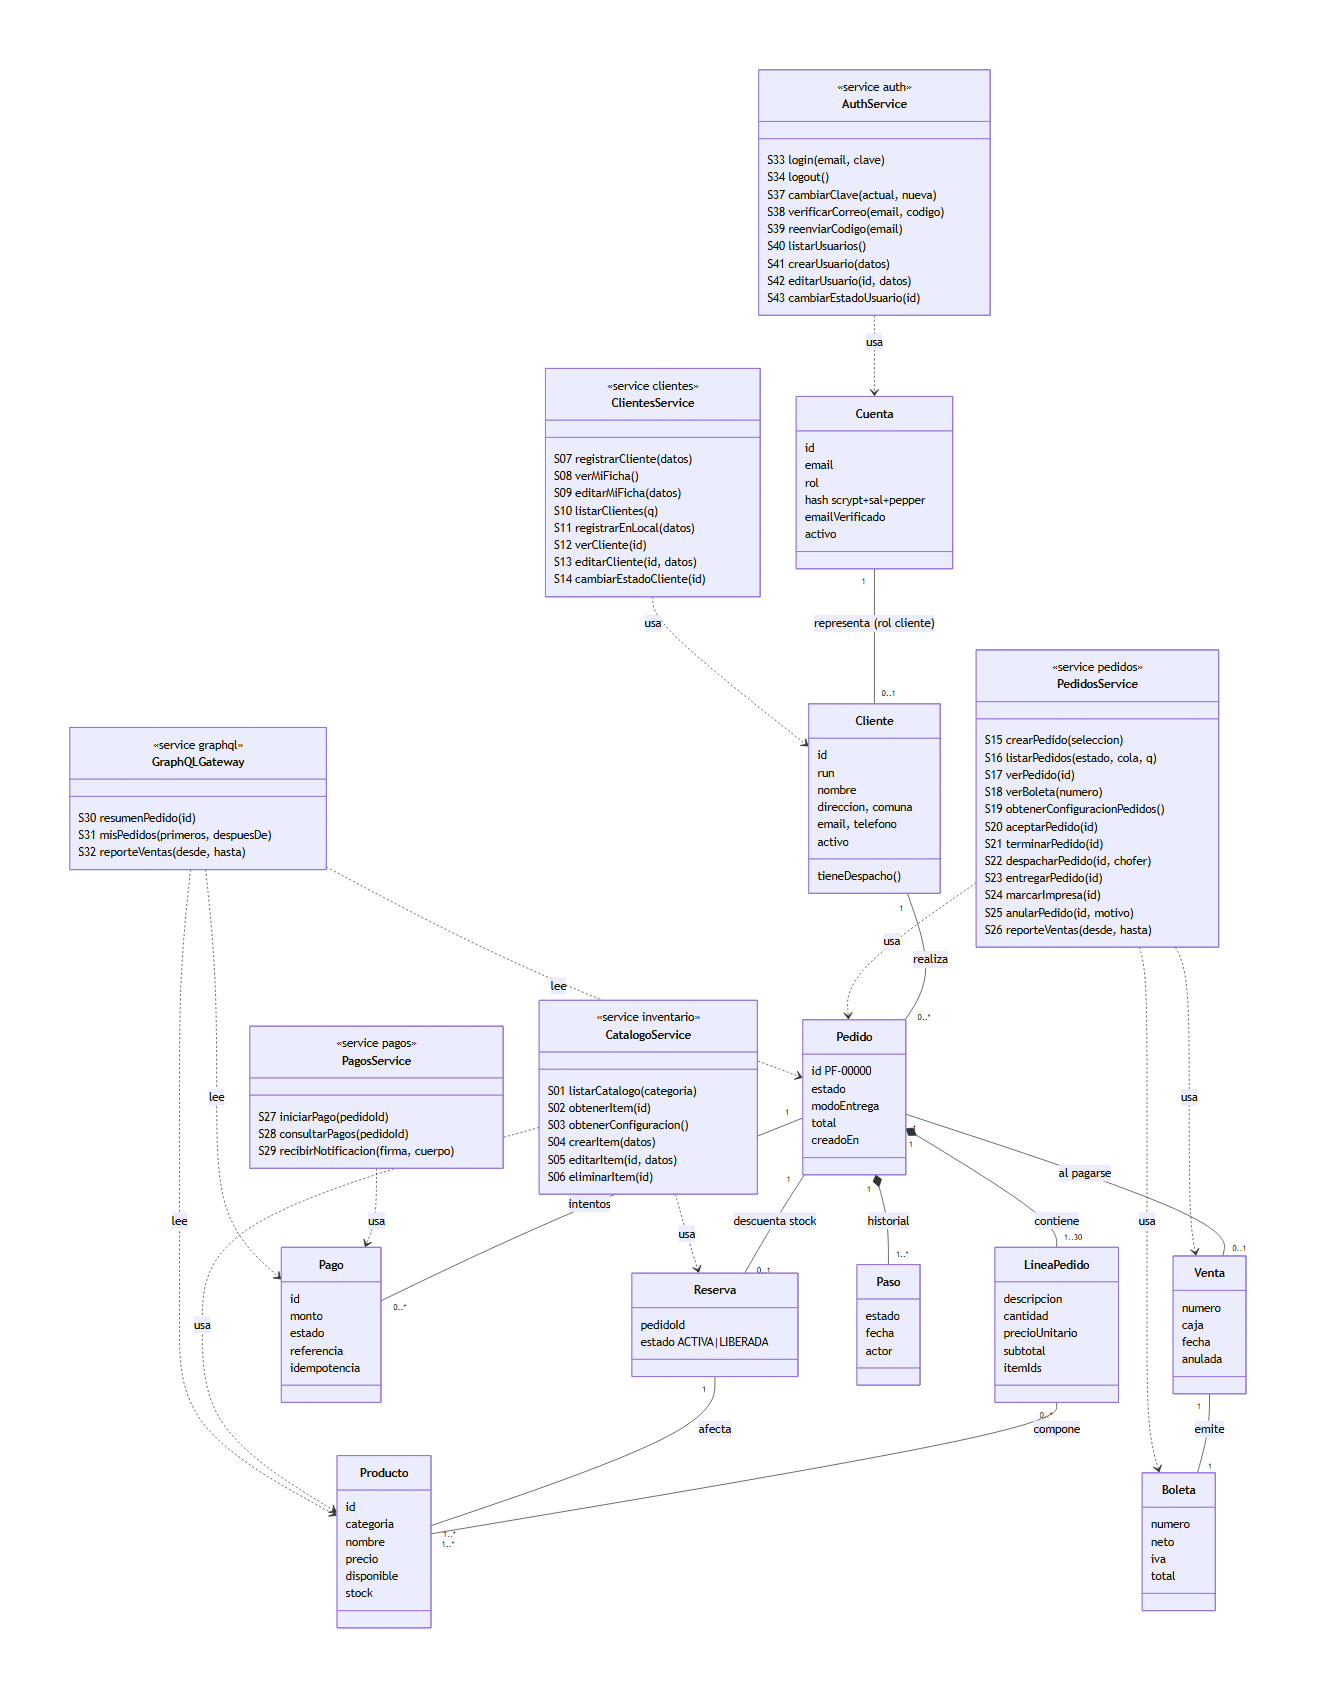
\includegraphics[width=\linewidth,height=0.8\textheight,keepaspectratio]{../diagramas/dominio.png}
\caption{UML del dominio y los servicios públicos}
\end{figure}

Editable: \texttt{diagramas/\allowbreak{}dominio.\allowbreak{}mmd} (Mermaid).


\subsection{Leyenda de notación y correspondencia con los servicios}

\begin{itemize}[nosep,leftmargin=*]
\item Una caja con \texttt{<<service .\allowbreak{}.\allowbreak{}.\allowbreak{}>>} es un servicio público: lista sus operaciones, cada una con el ID del módulo 1. El resto de las cajas son clases del dominio.
\item Una línea con rombo relleno es composición (la línea no existe sin el pedido: \texttt{Pedido} contiene sus líneas y sus pasos). Una línea simple es una asociación, con la multiplicidad en ambos extremos (\texttt{1}, \texttt{0.\allowbreak{}.\allowbreak{}1}, \texttt{0.\allowbreak{}.\allowbreak{}*}, \texttt{1.\allowbreak{}.\allowbreak{}*}).
\item Una flecha punteada (\texttt{.\allowbreak{}.\allowbreak{}>}) es una dependencia de uso: el servicio usa o lee esa clase. No significa que exista una instancia del servicio por cada registro.
\end{itemize}

{\small
\setlength{\tabcolsep}{3pt}\renewcommand{\arraystretch}{1.15}
\begin{longtable}{|>{\raggedright\arraybackslash}p{\dimexpr 0.2772\linewidth-2\tabcolsep\relax}|>{\raggedright\arraybackslash}p{\dimexpr 0.1948\linewidth-2\tabcolsep\relax}|>{\raggedright\arraybackslash}p{\dimexpr 0.2147\linewidth-2\tabcolsep\relax}|>{\raggedright\arraybackslash}p{\dimexpr 0.3133\linewidth-2\tabcolsep\relax}|}
\hline
\textbf{Clase \texttt{<<service>>}} & \textbf{Sistema} & \textbf{Operaciones (ID)} & \textbf{Clases del dominio que usa} \\ \hline
\endfirsthead
\hline
\textbf{Clase \texttt{<<service>>}} & \textbf{Sistema} & \textbf{Operaciones (ID)} & \textbf{Clases del dominio que usa} \\ \hline
\endhead
CatalogoService & inventario & S01 a S06 & Producto, Reserva \\ \hline
ClientesService & clientes & S07 a S14 & Cliente \\ \hline
PedidosService & pedidos & S15 a S26 & Pedido, LineaPedido, Paso, Venta, Boleta \\ \hline
PagosService & pagos & S27 a S29 & Pago \\ \hline
AuthService & Auth Service & S33, S34, S37 a S43 & Cuenta \\ \hline
GraphQLGateway & GraphQL Gateway & S30 a S32 & Pedido, Pago, Producto (solo lectura) \\ \hline
(API Gateway, sección 5) & gateway & S35, S36, S44 & — \\ \hline
\end{longtable}
}

\subsection{Cardinalidades y su regla de negocio}

{\small
\setlength{\tabcolsep}{3pt}\renewcommand{\arraystretch}{1.15}
\begin{longtable}{|>{\raggedright\arraybackslash}p{\dimexpr 0.2325\linewidth-2\tabcolsep\relax}|>{\raggedright\arraybackslash}p{\dimexpr 0.2392\linewidth-2\tabcolsep\relax}|>{\raggedright\arraybackslash}p{\dimexpr 0.5282\linewidth-2\tabcolsep\relax}|}
\hline
\textbf{Relación} & \textbf{Cardinalidad} & \textbf{Regla} \\ \hline
\endfirsthead
\hline
\textbf{Relación} & \textbf{Cardinalidad} & \textbf{Regla} \\ \hline
\endhead
Cuenta – Cliente & 1 a 0..1 & Toda ficha de cliente tiene exactamente una cuenta de rol cliente; las cuentas del personal no tienen ficha \\ \hline
Cliente – Pedido & 1 a 0..* & Solo clientes registrados compran (R7); un cliente puede no tener pedidos \\ \hline
Pedido – LineaPedido & 1 a 1..30 & Un pedido sin líneas no se crea; máximo 30 líneas y 20 unidades por línea (límite de abuso) \\ \hline
LineaPedido – Producto & 0..* a 1..* & Un bowl se compone de 2 o más productos (1 a 3 bases, 1 a 3 proteínas, hasta 4 salsas y 6 toppings); una bebida es 1 producto \\ \hline
Pedido – Paso (historial) & 1 a 1..* & Todo pedido nace con el paso PENDIENTE\_\allowbreak{}PAGO; cada cambio de estado agrega un paso \\ \hline
Pedido – Venta & 1 a 0..1 & La venta se registra solo cuando el pago se confirma, una sola vez \\ \hline
Venta – Boleta & 1 a 1 & El cajero virtual emite una boleta por venta (R8) \\ \hline
Pedido – Pago & 1 a 0..* & Puede haber intentos rechazados; a lo sumo uno aprobado \\ \hline
Pedido – Reserva & 1 a 0..1 & La reserva de stock se crea al confirmar el pedido y se libera al anular \\ \hline
\end{longtable}
}

\subsection{Decisiones de modelado}

\begin{itemize}[nosep,leftmargin=*]
\item \textbf{Carrito y pedido son cosas distintas.} El carrito existe solo en el navegador (\texttt{localStorage}) y es una selección sin precios confiables; el servidor no lo conoce. El pedido nace en S15, cuando el servidor cotiza y reserva. Por eso no hay una clase Carrito en el backend. No se modela un borrador de pedido: un pedido sin líneas no se crea (multiplicidad \texttt{1.\allowbreak{}.\allowbreak{}30}).
\item \textbf{Qué pasa con el historial si un producto deja de estar disponible.} Cada línea copia la descripción, el precio unitario y los \texttt{itemIds} al crear el pedido, y se relaciona con \texttt{Producto} solo por id. Desactivar o eliminar un producto (S05, S06) no cambia pedidos ni boletas ya emitidos. En el GraphQL, \texttt{Linea.\allowbreak{}productos} entrega solo los productos que aún existen (los demás se omiten) y el reporte por categoría los cuenta como \texttt{SIN\_\allowbreak{}CATEGORIA}.
\item \textbf{Qué se conserva y qué sale.} Internamente se guardan, por ejemplo, la clave de idempotencia y el consumo de stock del pedido, el \texttt{actor} de cada paso, el hash de la contraseña y el token de la pasarela; ninguno sale en una respuesta (sección de DTO, a continuación). El diagrama no muestra un campo solo porque exista en la base.
\end{itemize}

\subsection{Separación de DTO}

Cada servicio decide qué campos devuelve según quién pregunta, separando el documento guardado del objeto que viaja:


\begin{itemize}[nosep,leftmargin=*]
\item \textbf{inventario:} el público recibe \texttt{id,\allowbreak{} categoria,\allowbreak{} nombre,\allowbreak{} descripcion,\allowbreak{} precio,\allowbreak{} disponible} (disponible = activo y con stock). \texttt{stock} y \texttt{activo} solo para admin y dueño.
\item \textbf{pedidos:} cocina y despacho reciben del cliente solo \texttt{nombre} y \texttt{telefono}; el cliente recibe el historial sin el \texttt{actor} (quién del personal hizo cada paso); nunca salen \texttt{idempotencia} ni \texttt{consumo}.
\item \textbf{pagos:} nunca salen el \texttt{token} de la pasarela ni la clave de idempotencia; \texttt{urlPago} solo mientras el pago está pendiente.
\item \textbf{Auth Service:} nunca devuelve \texttt{hash} ni el código de verificación (se guarda solo su hash).
\item \textbf{clientes:} la ficha no guarda contraseña; la cuenta (en Auth) no guarda RUN ni dirección.
\end{itemize}

\subsection{Por qué estos límites}

{\footnotesize
\setlength{\tabcolsep}{3pt}\renewcommand{\arraystretch}{1.15}
\begin{longtable}{|>{\raggedright\arraybackslash}p{\dimexpr 0.1099\linewidth-2\tabcolsep\relax}|>{\raggedright\arraybackslash}p{\dimexpr 0.2458\linewidth-2\tabcolsep\relax}|>{\raggedright\arraybackslash}p{\dimexpr 0.2405\linewidth-2\tabcolsep\relax}|>{\raggedright\arraybackslash}p{\dimexpr 0.1232\linewidth-2\tabcolsep\relax}|>{\raggedright\arraybackslash}p{\dimexpr 0.2806\linewidth-2\tabcolsep\relax}|}
\hline
\textbf{Servicio} & \textbf{Cohesión} & \textbf{Acoplamiento} & \textbf{Propiedad de datos} & \textbf{Evolución} \\ \hline
\endfirsthead
\hline
\textbf{Servicio} & \textbf{Cohesión} & \textbf{Acoplamiento} & \textbf{Propiedad de datos} & \textbf{Evolución} \\ \hline
\endhead
inventario & Todo lo que define qué se vende y a qué precio & Lo consultan pedidos y GraphQL; no llama a nadie & Productos, stock, reservas & Cambiar recargos o agregar tamaños no toca pedidos \\ \hline
clientes & Datos personales del comprador & Llama a Auth para crear la cuenta & Fichas & Puede crecer (direcciones múltiples) sin tocar pedidos \\ \hline
pedidos & Ciclo de vida de la compra y documentos de venta & Llama a clientes, inventario y pagos & Pedidos, ventas, boletas & Nuevos estados o canales sin tocar pagos \\ \hline
pagos & Integración con el proveedor externo y dinero & Llama a pedidos y a la pasarela & Pagos & Cambiar de pasarela sin tocar pedidos \\ \hline
Auth Service & Credenciales y sesiones & Lo llaman gateway y clientes & Cuentas & Cambiar a OAuth/OIDC sin tocar los servicios \\ \hline
\end{longtable}
}

Cada servicio modifica solo su base. Las colaboraciones usan contratos explícitos (sección 6).


\clearpage
% Generado desde README.md. Editar libremente.

\section{3. Sistemas, componentes e integración}

\begin{landscape}
Cuatro sistemas se reparten el negocio: inventario (qué se vende y cuánto queda), pedidos (qué pasó con cada compra), clientes (quién compra) y pagos (el dinero). La regla de esta sección es que cada dato tenga un solo dueño, que es quien decide su estado oficial. La matriz dice qué hace cada sistema, de quién depende, con qué llave se lo llama y qué ocurre si falla; la secuencia de más abajo cuenta la compra de Javiera paso a paso.

\subsection{Matriz de sistemas}
Los cuatro sistemas mínimos del caso son microservicios privados, cada uno con su base y su usuario de Mongo. Cada uno decide el estado oficial de sus datos; los demás lo consultan por contrato.

\vspace{0.6em}
{\scriptsize
\setlength{\LTpre}{0pt}\setlength{\LTpost}{0pt}
\setlength{\tabcolsep}{3pt}\renewcommand{\arraystretch}{1.15}
\begin{longtable}{|>{\raggedright\arraybackslash}p{\dimexpr 0.0668\linewidth-2\tabcolsep\relax}|>{\raggedright\arraybackslash}p{\dimexpr 0.1465\linewidth-2\tabcolsep\relax}|>{\raggedright\arraybackslash}p{\dimexpr 0.1465\linewidth-2\tabcolsep\relax}|>{\raggedright\arraybackslash}p{\dimexpr 0.0540\linewidth-2\tabcolsep\relax}|>{\raggedright\arraybackslash}p{\dimexpr 0.1465\linewidth-2\tabcolsep\relax}|>{\raggedright\arraybackslash}p{\dimexpr 0.1465\linewidth-2\tabcolsep\relax}|>{\raggedright\arraybackslash}p{\dimexpr 0.1465\linewidth-2\tabcolsep\relax}|>{\raggedright\arraybackslash}p{\dimexpr 0.1465\linewidth-2\tabcolsep\relax}|}
\hline
\textbf{Sistema} & \textbf{Responsabilidad} & \textbf{Datos bajo su autoridad (estado oficial)} & \textbf{Servicios asociados} & \textbf{Dependencias} & \textbf{Contrato de integración} & \textbf{Credencial o identidad} & \textbf{Respuesta ante fallos} \\ \hline
\endfirsthead
\hline
\textbf{Sistema} & \textbf{Responsabilidad} & \textbf{Datos bajo su autoridad (estado oficial)} & \textbf{Servicios asociados} & \textbf{Dependencias} & \textbf{Contrato de integración} & \textbf{Credencial o identidad} & \textbf{Respuesta ante fallos} \\ \hline
\endhead
inventory (\texttt{inventario}) & Catálogo, precios, reglas de armado, cotización, stock y reservas & Producto, su precio y su disponibilidad; reservas (decide si hay unidades) & S01 a S06 & Ninguna: no llama a nadie & REST público (S01 a S06) y de integración: \texttt{POST /\allowbreak{}internos/\allowbreak{}cotizar}, \texttt{POST /\allowbreak{}internos/\allowbreak{}reservas}, \texttt{POST /\allowbreak{}internos/\allowbreak{}reservas/\allowbreak{}:\allowbreak{}pedido/\allowbreak{}liberar} & Recibe \texttt{X-\allowbreak{}Credencial-\allowbreak{}Interna} (\texttt{internos/\allowbreak{}inventario}); usuario de Mongo propio & Si no responde, pedidos no crea el pedido (\texttt{502/\allowbreak{}504}): nunca confirma sin cotizar. La reserva descuenta el stock ítem por ítem con la condición \texttt{stock >=\allowbreak{} cantidad} y, si uno no alcanza, devuelve lo ya descontado (\texttt{409 SIN\_\allowbreak{}STOCK}); es idempotente por pedido, se libera al anular y liberar dos veces devuelve el stock una sola vez \\ \hline
orders (\texttt{pedidos}) & Creación y ciclo de vida del pedido, venta, boleta, colas de cocina y despacho, reporte & Estado del pedido, venta y boleta (decide si un pedido está pagado, en preparación o entregado) & S15 a S26 & inventario (cotizar, reservar, liberar), clientes (ficha), pagos (devolución), ActiveMQ (publica) & REST público; interno \texttt{POST /\allowbreak{}internos/\allowbreak{}pedidos/\allowbreak{}:\allowbreak{}id/\allowbreak{}pago-\allowbreak{}confirmado}; eventos STOMP \texttt{/\allowbreak{}queue/\allowbreak{}correos} y \texttt{/\allowbreak{}queue/\allowbreak{}cocina} & Recibe \texttt{internos/\allowbreak{}pedidos}; usa las credenciales de inventario, clientes y pagos para llamarlos & Inventario o clientes caídos: \texttt{502/\allowbreak{}504}, no se crea nada. Falla de ActiveMQ: el pago se registra igual y el aviso queda en el log. Confirmar dos veces el mismo pago no hace nada la segunda vez \\ \hline
clients (\texttt{clientes}) & Registro, perfil y acceso autorizado a los datos del cliente & Ficha personal y si está activa (la cuenta y su verificación las decide Auth) & S07 a S14 & Auth Service (crear cuenta, cambiar estado, ver verificación) & REST público; interno \texttt{GET /\allowbreak{}internos/\allowbreak{}clientes/\allowbreak{}:\allowbreak{}id} (lo usa pedidos) & Recibe \texttt{internos/\allowbreak{}clientes}; ante Auth usa \texttt{internos/\allowbreak{}auth-\allowbreak{}clientes} (Basic, solo \texttt{/\allowbreak{}cuentas}) & Si Auth falla al registrar, se borra la ficha recién creada (compensación) y se responde el error. Si clientes no responde, pedidos responde \texttt{502/\allowbreak{}504} \\ \hline
payments (\texttt{pagos}) & Iniciar pagos, comprobar el resultado y relacionarse con el proveedor & Estado y monto del pago (el estado del \emph{pedido} lo decide pedidos) & S27 a S29 & pedidos (propiedad, monto y confirmación), pasarela (crear la transacción y devolver) & REST público; webhook firmado; interno \texttt{POST /\allowbreak{}internos/\allowbreak{}devoluciones} y \texttt{GET /\allowbreak{}internos/\allowbreak{}pagos} & Recibe \texttt{internos/\allowbreak{}pagos}; ante la pasarela usa \texttt{pasarela/\allowbreak{}comercio} (\texttt{api\_\allowbreak{}key}) y verifica \texttt{secreto\_\allowbreak{}firma} & Pasarela caída al iniciar: \texttt{502}. Si pedidos no responde al confirmar, se responde \texttt{502} y la pasarela reintenta (3 veces); la repetida reintenta solo el aviso a pedidos \\ \hline
\end{longtable}
}
\end{landscape}

\textbf{Quién autoriza el cambio de estado de un pago.} El aviso del proveedor se verifica en cuatro pasos: (1) firma HMAC-SHA256 del cuerpo exacto con el \texttt{secreto\_\allowbreak{}firma} que está en Vault; (2) el \texttt{token} y la orden corresponden a un pago registrado; (3) el monto coincide con el del pago (y pedidos vuelve a exigir que sea el total del pedido); (4) el cambio se aplica con una condición atómica (\texttt{estado:\allowbreak{} PENDIENTE} en el mismo \texttt{update}), de modo que una notificación repetida responde \texttt{repetido:\allowbreak{} true} sin registrar otra venta. Solo entonces pagos avisa a pedidos, y \textbf{pedidos es el único que cambia el estado del pedido a \texttt{PAGADO}}, emite la boleta y registra la venta. El frontend no decide nunca que un pedido está pagado: solo muestra lo que devuelve el servidor.


\textbf{orders e inventory.} Pedidos consulta a inventario, antes de aceptar el pedido, el precio y la disponibilidad de cada ítem (\texttt{cotizar}) y reserva las unidades (\texttt{reservas}). Si inventario no responde en 4~s, el pedido no se crea. Para no confirmar unidades que ya no existen, cada ítem se descuenta con una condición sobre el stock en la misma operación de actualización (\texttt{stock >=\allowbreak{} cantidad}), de modo que dos compras simultáneas no se llevan la misma unidad; si un ítem no alcanza, se devuelve lo ya descontado y el cliente recibe \texttt{SIN\_\allowbreak{}STOCK}.


\subsection{Estados del pedido y quién los cambia}

{\small
\setlength{\tabcolsep}{3pt}\renewcommand{\arraystretch}{1.15}
\begin{longtable}{|>{\raggedright\arraybackslash}p{\dimexpr 0.2178\linewidth-2\tabcolsep\relax}|>{\raggedright\arraybackslash}p{\dimexpr 0.2178\linewidth-2\tabcolsep\relax}|>{\raggedright\arraybackslash}p{\dimexpr 0.2251\linewidth-2\tabcolsep\relax}|>{\raggedright\arraybackslash}p{\dimexpr 0.3392\linewidth-2\tabcolsep\relax}|}
\hline
\textbf{Desde} & \textbf{Hacia} & \textbf{Operación (ID)} & \textbf{Quién} \\ \hline
\endfirsthead
\hline
\textbf{Desde} & \textbf{Hacia} & \textbf{Operación (ID)} & \textbf{Quién} \\ \hline
\endhead
(nuevo) & PENDIENTE\_\allowbreak{}PAGO & S15 & cliente \\ \hline
PENDIENTE\_\allowbreak{}PAGO & PAGADO & confirmación de pago (interna, desde S29) & pagos, con la credencial de pagos; el monto debe coincidir \\ \hline
PAGADO & EN\_\allowbreak{}PREPARACION & S20 & cocina, admin \\ \hline
EN\_\allowbreak{}PREPARACION & LISTO\_\allowbreak{}DESPACHO o LISTO\_\allowbreak{}RETIRO & S21 & cocina, admin \\ \hline
LISTO\_\allowbreak{}DESPACHO & EN\_\allowbreak{}DESPACHO & S22 & despacho, admin \\ \hline
EN\_\allowbreak{}DESPACHO o LISTO\_\allowbreak{}RETIRO & ENTREGADO & S23 & despacho, admin \\ \hline
PENDIENTE\_\allowbreak{}PAGO o PAGADO & ANULADO & S25 & cliente (suyo), admin \\ \hline
\end{longtable}
}

\subsection{Servicios propios y proveedores externos}

{\small
\setlength{\tabcolsep}{3pt}\renewcommand{\arraystretch}{1.15}
\begin{longtable}{|>{\raggedright\arraybackslash}p{\dimexpr 0.1840\linewidth-2\tabcolsep\relax}|>{\raggedright\arraybackslash}p{\dimexpr 0.2324\linewidth-2\tabcolsep\relax}|>{\raggedright\arraybackslash}p{\dimexpr 0.4128\linewidth-2\tabcolsep\relax}|>{\raggedright\arraybackslash}p{\dimexpr 0.1707\linewidth-2\tabcolsep\relax}|}
\hline
\textbf{Pieza} & \textbf{Propia o externa} & \textbf{Qué hace} & \textbf{Cómo se prueba} \\ \hline
\endfirsthead
\hline
\textbf{Pieza} & \textbf{Propia o externa} & \textbf{Qué hace} & \textbf{Cómo se prueba} \\ \hline
\endhead
Despacho & Propia (dentro de pedidos) & Cola, chofer y entrega; comparte el estado del pedido, por eso no se separa en otro servicio & Caso 10.4 \\ \hline
Boleta y cajero virtual & Propia (dentro de pedidos) & La venta y la boleta se emiten en la misma operación atómica que confirma el pago & Casos 10.2 y 10.3 \\ \hline
Mensajería & Propia (ActiveMQ + notificador) & Boleta al correo y aviso a cocina, sin bloquear el pago & Log del notificador \\ \hline
Pasarela de pagos (Servipag) & \textbf{Externa, simulada} & Cobrar, notificar y devolver & Casos 7.6, 10.2 y 10.3 \\ \hline
Correo & \textbf{Externo, simulado} & Entregar el correo; en modo demo se muestra en pantalla & Brecha declarada \\ \hline
\end{longtable}
}

\subsection{Sistemas de soporte}

{\footnotesize
\setlength{\tabcolsep}{3pt}\renewcommand{\arraystretch}{1.15}
\begin{longtable}{|>{\raggedright\arraybackslash}p{\dimexpr 0.0965\linewidth-2\tabcolsep\relax}|>{\raggedright\arraybackslash}p{\dimexpr 0.1151\linewidth-2\tabcolsep\relax}|>{\raggedright\arraybackslash}p{\dimexpr 0.1909\linewidth-2\tabcolsep\relax}|>{\raggedright\arraybackslash}p{\dimexpr 0.1757\linewidth-2\tabcolsep\relax}|>{\raggedright\arraybackslash}p{\dimexpr 0.1676\linewidth-2\tabcolsep\relax}|>{\raggedright\arraybackslash}p{\dimexpr 0.2541\linewidth-2\tabcolsep\relax}|}
\hline
\textbf{Sistema} & \textbf{Tipo} & \textbf{Protocolo} & \textbf{Lo usa} & \textbf{Datos que intercambia} & \textbf{Si falla} \\ \hline
\endfirsthead
\hline
\textbf{Sistema} & \textbf{Tipo} & \textbf{Protocolo} & \textbf{Lo usa} & \textbf{Datos que intercambia} & \textbf{Si falla} \\ \hline
\endhead
MongoDB 7 & Persistencia & Mongo wire sobre TLS, usuario por servicio & Auth, inventario, clientes, pedidos, pagos & Documentos de cada servicio & El servicio responde 500; \texttt{/\allowbreak{}salud} lo informa \\ \hline
HashiCorp Vault 1.18 & Secretos & HTTPS (KV v2) con token por servicio & Todos los servicios & Credenciales, pepper, claves & Se usa lo leído hasta 5 min; después 503 (no se deja pasar a nadie) \\ \hline
ActiveMQ Classic 6 & Mensajería & STOMP 1.2 sobre TLS & pedidos (publica), notificador (consume) & Boleta para correo, aviso a cocina & El pago se registra igual; queda en el log \\ \hline
Pasarela (Servipag) & Externo & HTTPS + API key; notificación con HMAC & pagos & Transacción, resultado, devolución & Pagar responde 502; la pasarela reintenta la notificación 3 veces \\ \hline
\end{longtable}
}

\subsection{Mapa de componentes y despliegue}

\begin{figure}[H]
\centering
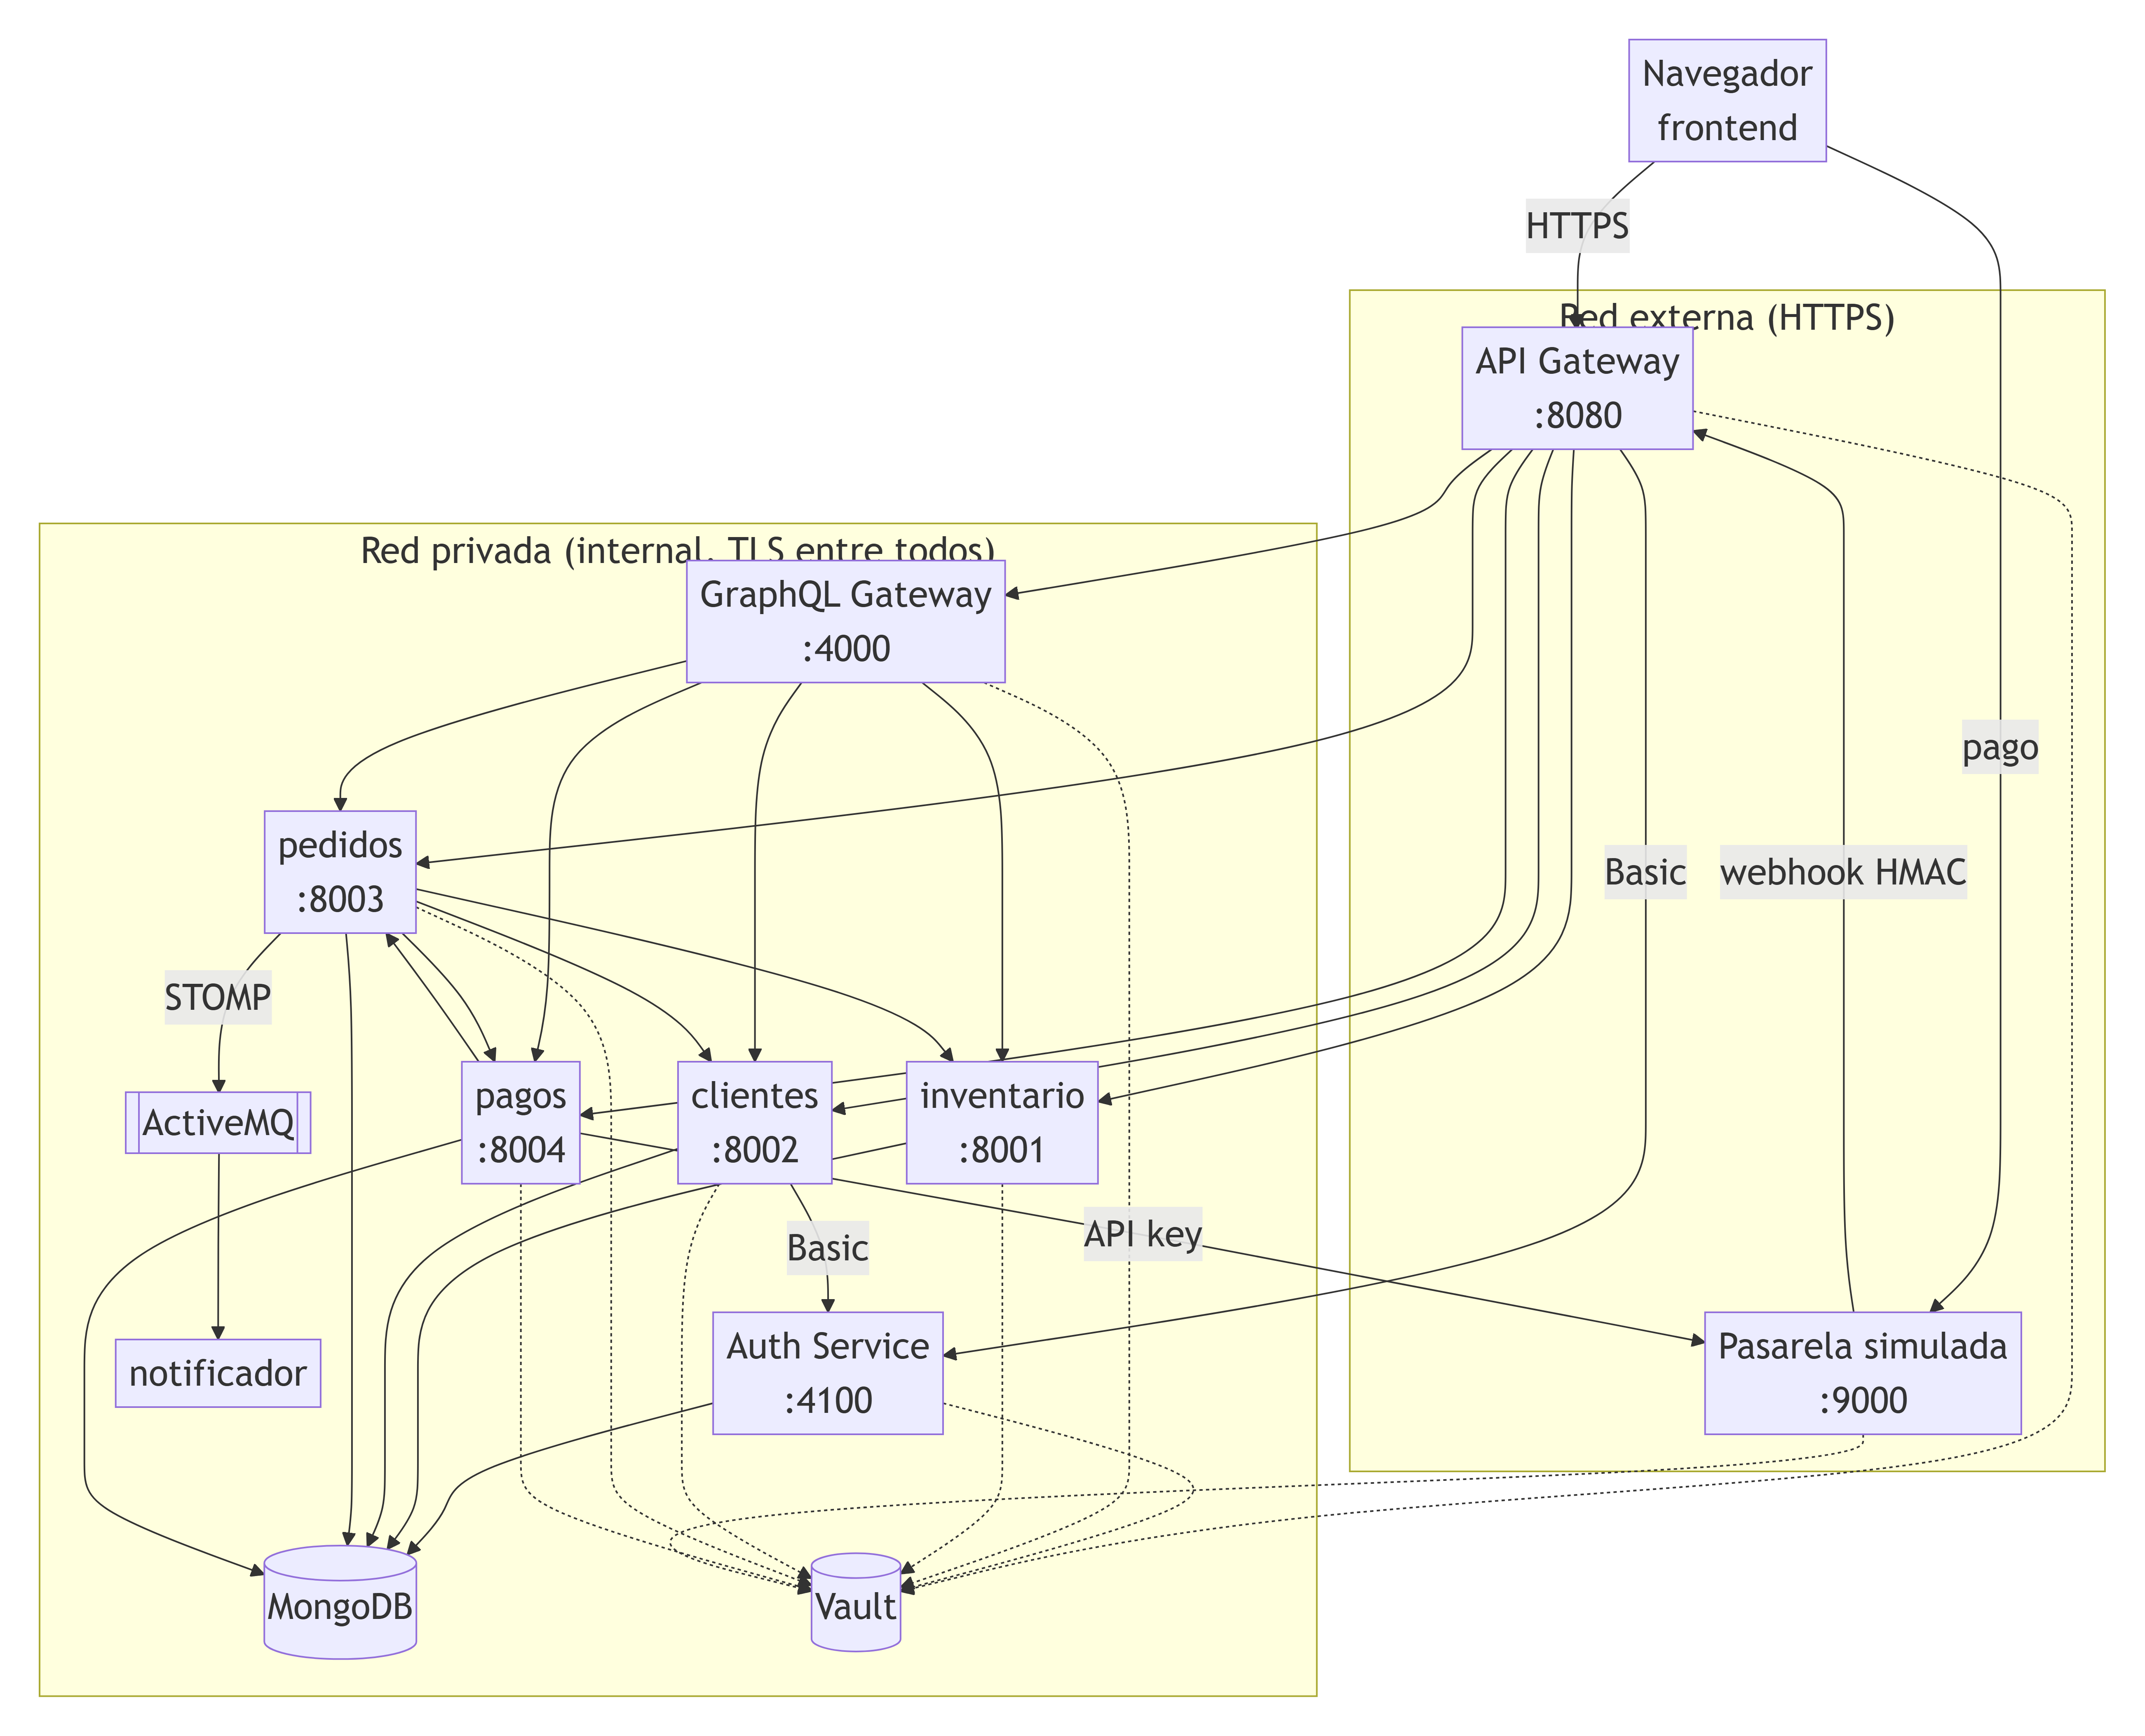
\includegraphics[width=\linewidth,height=0.85\textheight,keepaspectratio]{../diagramas/componentes.png}
\caption{Mapa de componentes}
\end{figure}

Leyenda: las flechas continuas son llamadas entre componentes (todas por TLS 1.2 o superior); \texttt{Basic} es HTTP Basic con un secreto de Vault, \texttt{API key} es la clave del comercio ante la pasarela y \texttt{webhook HMAC} es la notificación firmada; las líneas punteadas son la lectura de secretos en Vault, cada componente con su propio token; \texttt{STOMP} es la mensajería hacia ActiveMQ. El detalle de qué se verifica en cada salto está en la tabla de fronteras de confianza (sección 5).


Modelo C4 (\texttt{docs/\allowbreak{}diagramas/\allowbreak{}poke-\allowbreak{}fresh.\allowbreak{}dsl}): 25 vistas, validadas con el comando \texttt{validate} de Structurizr (imagen \texttt{structurizr/\allowbreak{}structurizr}) y exportables a Mermaid. Incluye C1 (contexto con la pasarela externa), C2 (contenedores, con recortes de catálogo, pedidos y pagos, y secretos), C3 de API Gateway, GraphQL Gateway, Auth Service y pedidos, vistas dinámicas de los flujos de los casos de validación (catálogo y su recuperación, pedido y su reintento, pedido propio y ajeno, sesión expirada, GraphQL con éxito, con error parcial y sobre el límite, pago, confirmación firmada y notificación falsa) y dos despliegues: \texttt{Docker\_\allowbreak{}Compose} (el entregado) y \texttt{Local\_\allowbreak{}Sin\_\allowbreak{}Docker} (pruebas, con Mongo, Vault y ActiveMQ en memoria). Para verlo: pegar el archivo en https://structurizr.com/dsl o usar el CLI. No hay imágenes renderizadas de estas vistas en el repositorio; los \texttt{.\allowbreak{}png} de arriba siguen siendo los diagramas de referencia del informe.


Despliegue (\texttt{docker-\allowbreak{}compose.\allowbreak{}yml}): 15 contenedores en dos redes (\texttt{tls-\allowbreak{}init}, \texttt{vault-\allowbreak{}init} y \texttt{semilla} son de un solo uso: crean los certificados, los secretos y los datos de ejemplo, respectivamente). \texttt{privada} es \texttt{internal:\allowbreak{} true} (sin puertos al equipo ni salida a Internet). Solo el gateway (8080) y la pasarela simulada (9000) publican puertos.


\begin{landscape}
\subsection{Secuencia de integración: compra completa}
\begin{figure}[H]
\centering
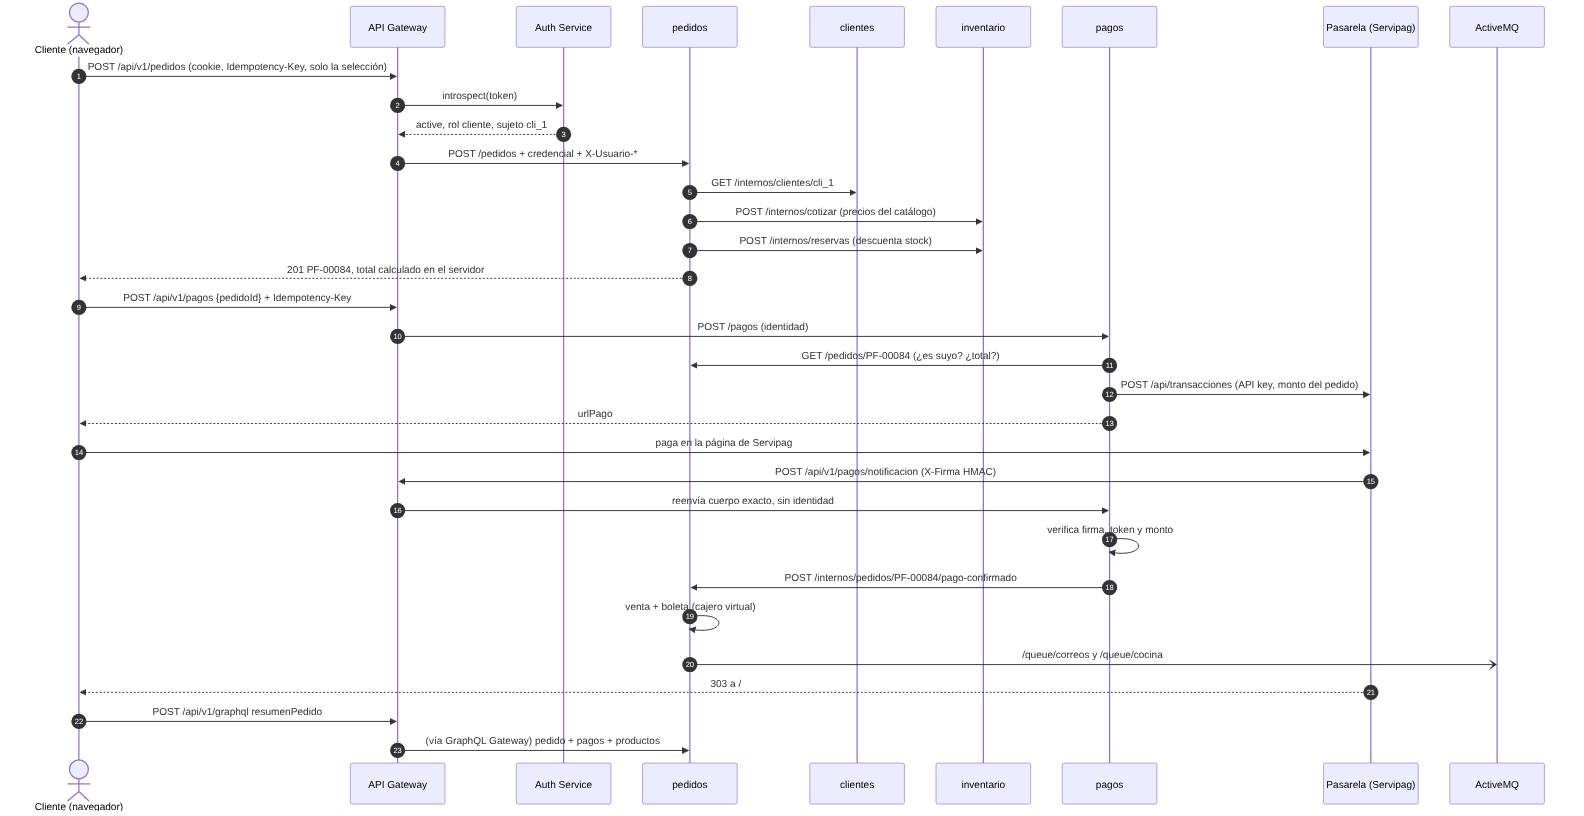
\includegraphics[width=\linewidth,height=0.78\textheight,keepaspectratio]{../diagramas/secuencia-compra.png}
\caption{Secuencia de compra}
\end{figure}
\end{landscape}

\subsection{Idempotencia del pago}

\begin{itemize}[nosep,leftmargin=*]
\item \textbf{Crear pedido:} \texttt{Idempotency-\allowbreak{}Key} opcional; el frontend genera una por visita a la pantalla de confirmación. Un doble clic devuelve el mismo pedido (índice único \texttt{idempotencia}).
\item \textbf{Iniciar pago:} \texttt{Idempotency-\allowbreak{}Key} obligatoria; misma clave $\rightarrow$ mismo pago. Si ya hay un pago pendiente para el pedido, se reutiliza.
\item \textbf{Notificación:} se aplica con una condición atómica (\texttt{estado:\allowbreak{} PENDIENTE} en el mismo \texttt{update}). Una repetida responde \texttt{repetido:\allowbreak{} true} sin volver a registrar la venta. Si pedidos no respondió la primera vez, la repetida reintenta solo ese aviso.
\item \textbf{Confirmación en pedidos:} si llega dos veces el mismo \texttt{pagoId}, la segunda no hace nada; el monto debe ser exactamente el total.
\item \textbf{Reservas de stock:} una por pedido; liberar dos veces devuelve el stock una sola vez.
\end{itemize}

Probado en \texttt{servicios/\allowbreak{}tests/\allowbreak{}test\_\allowbreak{}pedidos\_\allowbreak{}y\_\allowbreak{}pagos.\allowbreak{}py} y en los casos 10.2 y 10.3 de punta a punta.


\clearpage
% Generado desde README.md. Editar libremente.

\section{4. Stakeholders y matriz de permisos}

Un sistema seguro no solo pregunta quién eres, también qué puedes hacer. Aquí se describe quiénes usan Poke Fresh (clientes, personal del local, la pasarela de pago, el equipo de TI) y qué puede hacer cada uno con cada servicio. Para cada operación hay una decisión por rol y, cuando corresponde, una condición: por ejemplo, un cliente puede ver pedidos, pero solo los suyos.


\subsection{Stakeholders}

{\small
\setlength{\tabcolsep}{3pt}\renewcommand{\arraystretch}{1.15}
\begin{longtable}{|>{\raggedright\arraybackslash}p{\dimexpr 0.1652\linewidth-2\tabcolsep\relax}|>{\raggedright\arraybackslash}p{\dimexpr 0.1478\linewidth-2\tabcolsep\relax}|>{\raggedright\arraybackslash}p{\dimexpr 0.3435\linewidth-2\tabcolsep\relax}|>{\raggedright\arraybackslash}p{\dimexpr 0.3435\linewidth-2\tabcolsep\relax}|}
\hline
\textbf{Stakeholder} & \textbf{Interés} & \textbf{Qué puede hacer} & \textbf{Qué protege el sistema de él} \\ \hline
\endfirsthead
\hline
\textbf{Stakeholder} & \textbf{Interés} & \textbf{Qué puede hacer} & \textbf{Qué protege el sistema de él} \\ \hline
\endhead
Visitante & Ver el menú y precios & Catálogo, registrarse & Datos de clientes y pedidos \\ \hline
Cliente & Comprar, seguir su pedido & Sus pedidos, su ficha, pagar, anular antes de cocina & Pedidos y datos de otros clientes; fijar precios o confirmar pagos \\ \hline
Administrador & Operar todo el local & Todo el panel & Desactivarse a sí mismo o dejar el local sin administrador \\ \hline
Dueño & Ventas y productos & Reportes, caja, productos (sin eliminar) & Datos de clientes y gestión de usuarios \\ \hline
Cocina & Preparar en orden & Cola de cocina, aceptar, terminar & Reportes, RUN y correo de los clientes \\ \hline
Encargado de despacho & Entregar & Cola de despacho, chofer, entrega & Reportes, RUN y correo \\ \hline
Servipag & Cobrar & Notificar resultados firmados & Notificar sin la firma, o con otro monto \\ \hline
Equipo de TI & Operar y auditar & \textbf{Sin permisos operativos} en la aplicación: no tiene rol ni cuenta; recibe información por los logs con \texttt{X-\allowbreak{}Request-\allowbreak{}Id} y \texttt{/\allowbreak{}api/\allowbreak{}salud} (S44) & Ver contraseñas, tokens o cuerpos en los logs \\ \hline
\end{longtable}
}

\subsection{Partes interesadas, roles e identidades técnicas}

{\small
\setlength{\tabcolsep}{3pt}\renewcommand{\arraystretch}{1.15}
\begin{longtable}{|>{\raggedright\arraybackslash}p{\dimexpr 0.2633\linewidth-2\tabcolsep\relax}|>{\raggedright\arraybackslash}p{\dimexpr 0.3639\linewidth-2\tabcolsep\relax}|>{\raggedright\arraybackslash}p{\dimexpr 0.3728\linewidth-2\tabcolsep\relax}|}
\hline
\textbf{Categoría} & \textbf{Quiénes} & \textbf{Cómo se representan} \\ \hline
\endfirsthead
\hline
\textbf{Categoría} & \textbf{Quiénes} & \textbf{Cómo se representan} \\ \hline
\endhead
Roles de usuario (con permisos operativos) & Cliente, administrador, dueño, cocina, encargado de despacho & Cuentas en el Auth Service con un perfil; el gateway aplica el rol y el servicio dueño aplica la propiedad \\ \hline
Parte interesada sin permisos operativos & Equipo de TI & Sin cuenta ni rol. Recibe información por logs y \texttt{/\allowbreak{}api/\allowbreak{}salud}; nunca por la API de negocio. Ver contraseñas o tokens en los logs está excluido \\ \hline
Identidades técnicas & Servipag (webhook), gateway, cada servicio, notificador & Servipag se autentica con la firma del cuerpo; los componentes internos, con su credencial de servicio y su token de Vault (sección 6) \\ \hline
Visitante & Quien aún no ingresa & Sin identidad: solo operaciones públicas (S01 a S03, S07, S33, S35, S36, S38, S39) \\ \hline
\end{longtable}
}

La autenticación (quién eres) la hace el Auth Service por introspección del token; la autorización (qué puedes hacer) la decide el gateway por rol y el servicio dueño por propiedad y estado.


\subsection{Por qué los permisos son así}

\begin{itemize}[nosep,leftmargin=*]
\item \textbf{Cada rol recibe lo mínimo que necesita para hacer su trabajo.} Cocina necesita saber qué preparar y a quién avisar: ve el nombre y el teléfono del cliente, pero no su RUN ni su correo. Despacho ve su cola y la dirección de entrega. El dueño mira ventas y productos, pero no administra usuarios.
\item \textbf{Hay dos candados, no uno.} El gateway comprueba el rol (un cliente no puede entrar al panel de cocina) y el servicio dueño del dato vuelve a comprobar la regla fina, como que un pedido sea de quien lo pide. Si alguien llegara a un servicio por otro camino, el segundo candado igual diría que no.
\item \textbf{Un pedido ajeno se responde como inexistente.} Cuando un cliente pide el pedido de otra persona, el servicio contesta 404 y no 403: un “prohibido” confirmaría que ese pedido existe.
\item \textbf{Siempre queda alguien a cargo.} El sistema no deja desactivar al último administrador ni que alguien cambie su propio perfil, para que nadie se quede sin acceso por un error.
\item \textbf{Ocultar un botón no es un permiso.} Lo que importa es lo que el backend responde, y por eso las pruebas de la sección 7 se hacen contra el backend, no contra la pantalla.
\end{itemize}

\begin{landscape}
\subsection{Permisos por rol y servicio}
Decisión por rol y por ID de servicio (la ruta y el verbo son los del módulo 1). \textbf{Sí}: permitido. \textbf{Sí*}: permitido solo si se cumple la condición de la última columna. \textbf{No}: denegado (el gateway responde 403, o 401 si no hay sesión). El control grueso (rol) lo aplica el gateway con la matriz de rutas; la condición la aplica el servicio dueño del dato y se vuelve a comprobar ahí. Esta tabla se generó leyendo \texttt{gateway/\allowbreak{}src/\allowbreak{}rutas.\allowbreak{}js}, así que no puede contradecir al código.

\vspace{0.6em}
{\scriptsize
\setlength{\LTpre}{0pt}\setlength{\LTpost}{0pt}
\setlength{\tabcolsep}{3pt}\renewcommand{\arraystretch}{1.15}
\begin{longtable}{|>{\raggedright\arraybackslash}p{\dimexpr 0.0510\linewidth-2\tabcolsep\relax}|>{\raggedright\arraybackslash}p{\dimexpr 0.1432\linewidth-2\tabcolsep\relax}|>{\raggedright\arraybackslash}p{\dimexpr 0.0940\linewidth-2\tabcolsep\relax}|>{\raggedright\arraybackslash}p{\dimexpr 0.0797\linewidth-2\tabcolsep\relax}|>{\raggedright\arraybackslash}p{\dimexpr 0.0725\linewidth-2\tabcolsep\relax}|>{\raggedright\arraybackslash}p{\dimexpr 0.0869\linewidth-2\tabcolsep\relax}|>{\raggedright\arraybackslash}p{\dimexpr 0.0653\linewidth-2\tabcolsep\relax}|>{\raggedright\arraybackslash}p{\dimexpr 0.0653\linewidth-2\tabcolsep\relax}|>{\raggedright\arraybackslash}p{\dimexpr 0.0869\linewidth-2\tabcolsep\relax}|>{\raggedright\arraybackslash}p{\dimexpr 0.2552\linewidth-2\tabcolsep\relax}|}
\hline
\textbf{ID} & \textbf{Verbo y ruta (\texttt{/\allowbreak{}api/\allowbreak{}v1})} & \textbf{Visitante} & \textbf{Cliente} & \textbf{Cocina} & \textbf{Despacho} & \textbf{Dueño} & \textbf{Admin} & \textbf{Servipag} & \textbf{Alcance y condición} \\ \hline
\endfirsthead
\hline
\textbf{ID} & \textbf{Verbo y ruta (\texttt{/\allowbreak{}api/\allowbreak{}v1})} & \textbf{Visitante} & \textbf{Cliente} & \textbf{Cocina} & \textbf{Despacho} & \textbf{Dueño} & \textbf{Admin} & \textbf{Servipag} & \textbf{Alcance y condición} \\ \hline
\endhead
S01 & \texttt{GET /\allowbreak{}catalogo/\allowbreak{}items} & Sí & Sí & Sí & Sí & Sí & Sí & No & Stock y \texttt{activo} solo se ven como admin o dueño \\ \hline
S02 & \texttt{GET /\allowbreak{}catalogo/\allowbreak{}items/\allowbreak{}:\allowbreak{}id} & Sí & Sí & Sí & Sí & Sí & Sí & No & Igual que S01 \\ \hline
S03 & \texttt{GET /\allowbreak{}catalogo/\allowbreak{}configuracion} & Sí & Sí & Sí & Sí & Sí & Sí & No & — \\ \hline
S04 & \texttt{POST /\allowbreak{}catalogo/\allowbreak{}items} & No & No & No & No & Sí & Sí & No & Nombre único; precio y stock válidos \\ \hline
S05 & \texttt{PUT /\allowbreak{}catalogo/\allowbreak{}items/\allowbreak{}:\allowbreak{}id} & No & No & No & No & Sí & Sí & No & Nombre único; precio y stock válidos \\ \hline
S06 & \texttt{DELETE /\allowbreak{}catalogo/\allowbreak{}items/\allowbreak{}:\allowbreak{}id} & No & No & No & No & No & Sí & No & Solo admin (inventario lo vuelve a comprobar) \\ \hline
S07 & \texttt{POST /\allowbreak{}clientes/\allowbreak{}registro} & Sí & Sí & Sí & Sí & Sí & Sí & No & RUN con dígito verificador y único; correo único; clave fuerte \\ \hline
S08 & \texttt{GET /\allowbreak{}clientes/\allowbreak{}yo} & No & Sí* & No & No & No & No & No & Solo su ficha (\texttt{X-\allowbreak{}Usuario-\allowbreak{}Sujeto}) \\ \hline
S09 & \texttt{PUT /\allowbreak{}clientes/\allowbreak{}yo} & No & Sí* & No & No & No & No & No & Solo su ficha; no cambia RUN ni estado \\ \hline
S10 & \texttt{GET /\allowbreak{}clientes} & No & No & No & No & No & Sí & No & — \\ \hline
S11 & \texttt{POST /\allowbreak{}clientes} & No & No & No & No & No & Sí & No & RUN y correo únicos; clave temporal generada por el servidor \\ \hline
S12 & \texttt{GET /\allowbreak{}clientes/\allowbreak{}:\allowbreak{}id} & No & No & No & No & No & Sí & No & — \\ \hline
S13 & \texttt{PUT /\allowbreak{}clientes/\allowbreak{}:\allowbreak{}id} & No & No & No & No & No & Sí & No & — \\ \hline
S14 & \texttt{PATCH /\allowbreak{}clientes/\allowbreak{}:\allowbreak{}id/\allowbreak{}estado} & No & No & No & No & No & Sí & No & Desactivar cierra sus sesiones \\ \hline
S15 & \texttt{POST /\allowbreak{}pedidos} & No & Sí* & No & No & No & No & No & Cuenta activa; despacho solo en las comunas de reparto; precio de inventario; stock \\ \hline
S16 & \texttt{GET /\allowbreak{}pedidos} & No & Sí* & Sí* & Sí* & Sí & Sí & No & Cliente: solo los suyos. Cocina y despacho: solo su cola \\ \hline
S17 & \texttt{GET /\allowbreak{}pedidos/\allowbreak{}:\allowbreak{}id} & No & Sí* & Sí* & Sí* & Sí & Sí & No & Cliente: solo si es suyo (si no, 404). Cocina: solo pagados. Despacho: solo listos, en camino o entregados \\ \hline
S18 & \texttt{GET /\allowbreak{}pedidos/\allowbreak{}boleta/\allowbreak{}:\allowbreak{}numero} & No & Sí* & No & No & Sí & Sí & No & Cliente: solo la suya \\ \hline
S19 & \texttt{GET /\allowbreak{}pedidos/\allowbreak{}configuracion} & No & Sí & Sí & Sí & Sí & Sí & No & — \\ \hline
S20 & \texttt{POST /\allowbreak{}pedidos/\allowbreak{}:\allowbreak{}id/\allowbreak{}aceptar} & No & No & Sí* & No & No & Sí* & No & Solo desde PAGADO; condición atómica \\ \hline
S21 & \texttt{POST /\allowbreak{}pedidos/\allowbreak{}:\allowbreak{}id/\allowbreak{}terminar} & No & No & Sí* & No & No & Sí* & No & Solo desde EN\_\allowbreak{}PREPARACION; condición atómica \\ \hline
S22 & \texttt{POST /\allowbreak{}pedidos/\allowbreak{}:\allowbreak{}id/\allowbreak{}despachar} & No & No & No & Sí* & No & Sí* & No & Solo desde LISTO\_\allowbreak{}DESPACHO; chofer de la lista \\ \hline
S23 & \texttt{POST /\allowbreak{}pedidos/\allowbreak{}:\allowbreak{}id/\allowbreak{}entregar} & No & No & No & Sí* & No & Sí* & No & Solo desde EN\_\allowbreak{}DESPACHO o LISTO\_\allowbreak{}RETIRO \\ \hline
S24 & \texttt{POST /\allowbreak{}pedidos/\allowbreak{}:\allowbreak{}id/\allowbreak{}impresa} & No & No & Sí & Sí & No & Sí & No & — \\ \hline
S25 & \texttt{POST /\allowbreak{}pedidos/\allowbreak{}:\allowbreak{}id/\allowbreak{}anular} & No & Sí* & No & No & No & Sí* & No & Cliente: solo el suyo. Solo en PENDIENTE\_\allowbreak{}PAGO o PAGADO; motivo de 5 a 200 caracteres \\ \hline
S26 & \texttt{GET /\allowbreak{}reportes/\allowbreak{}ventas} & No & No & No & No & Sí & Sí & No & Período máximo de un año \\ \hline
S27 & \texttt{POST /\allowbreak{}pagos} & No & Sí* & No & No & No & No & No & Pedido suyo y pendiente (lo decide pedidos); monto del pedido; \texttt{Idempotency-\allowbreak{}Key} \\ \hline
S28 & \texttt{GET /\allowbreak{}pagos} & No & Sí* & No & No & Sí & Sí & No & Pedidos decide si puede ver ese pedido \\ \hline
S29 & \texttt{POST /\allowbreak{}pagos/\allowbreak{}notificacion} & No & No & No & No & No & No & Sí (firma) & Firma HMAC válida; token y monto coinciden \\ \hline
S30 & \texttt{POST /\allowbreak{}graphql} \texttt{resumenPedido} & No & Sí* & Sí* & Sí* & Sí & Sí & No & Cliente: solo si el pedido es suyo. Cocina y despacho: según su cola. Campo \texttt{cliente}: solo admin \\ \hline
S31 & \texttt{POST /\allowbreak{}graphql} \texttt{misPedidos} & No & Sí* & No & No & No & No & No & Solo los pedidos del propio cliente \\ \hline
S32 & \texttt{POST /\allowbreak{}graphql} \texttt{reporteVentas} & No & No & No & No & Sí & Sí & No & Solo admin y dueño \\ \hline
S33 & \texttt{POST /\allowbreak{}auth/\allowbreak{}login} & Sí & Sí & Sí & Sí & Sí & Sí & No & 20 por minuto por IP; bloqueo por correo tras 5 intentos fallidos \\ \hline
S34 & \texttt{POST /\allowbreak{}auth/\allowbreak{}logout} & Sí & Sí & Sí & Sí & Sí & Sí & No & — \\ \hline
S35 & \texttt{GET /\allowbreak{}auth/\allowbreak{}sesion} & Sí & Sí & Sí & Sí & Sí & Sí & No & Sin sesión responde \texttt{null} \\ \hline
S36 & \texttt{GET /\allowbreak{}auth/\allowbreak{}config} & Sí & Sí & Sí & Sí & Sí & Sí & No & Sin cuentas de demostración si \texttt{MODO\_\allowbreak{}DEMO=\allowbreak{}false} \\ \hline
S37 & \texttt{PUT /\allowbreak{}auth/\allowbreak{}clave} & No & Sí & Sí & Sí & Sí & Sí & No & La cuenta sale de la sesión, no del cuerpo \\ \hline
S38 & \texttt{POST /\allowbreak{}auth/\allowbreak{}verificar} & Sí & Sí & Sí & Sí & Sí & Sí & No & 20 por minuto por IP; no revela si el correo existe \\ \hline
S39 & \texttt{POST /\allowbreak{}auth/\allowbreak{}reenviar} & Sí & Sí & Sí & Sí & Sí & Sí & No & 20 por minuto por IP; respuesta igual exista o no el correo \\ \hline
S40 & \texttt{GET /\allowbreak{}usuarios} & No & No & No & No & No & Sí & No & — \\ \hline
S41 & \texttt{POST /\allowbreak{}usuarios} & No & No & No & No & No & Sí & No & Clave fuerte; perfil válido \\ \hline
S42 & \texttt{PUT /\allowbreak{}usuarios/\allowbreak{}:\allowbreak{}id} & No & No & No & No & No & Sí* & No & Siempre queda un admin activo; nadie cambia su propio perfil \\ \hline
S43 & \texttt{PATCH /\allowbreak{}usuarios/\allowbreak{}:\allowbreak{}id/\allowbreak{}estado} & No & No & No & No & No & Sí* & No & Siempre queda un admin activo; nadie desactiva su propia cuenta \\ \hline
S44 & \texttt{GET /\allowbreak{}api/\allowbreak{}salud} & Sí & Sí & Sí & Sí & Sí & Sí & No & Sin datos personales \\ \hline
\end{longtable}
}
\end{landscape}

La columna Servipag es la identidad técnica de la pasarela: no tiene sesión ni rol; su único permiso es S29, autenticado con la firma del cuerpo. Las identidades técnicas internas (gateway, servicios, notificador) no figuran aquí porque no usan estas rutas públicas: se autentican entre sí con las credenciales de la sección 6.


\textbf{Verbos por recurso.} “No aplicable” significa que la operación no existe (404 o 405), no que se deniegue:


{\footnotesize
\setlength{\tabcolsep}{3pt}\renewcommand{\arraystretch}{1.15}
\begin{longtable}{|>{\raggedright\arraybackslash}p{\dimexpr 0.0947\linewidth-2\tabcolsep\relax}|>{\raggedright\arraybackslash}p{\dimexpr 0.1409\linewidth-2\tabcolsep\relax}|>{\raggedright\arraybackslash}p{\dimexpr 0.2353\linewidth-2\tabcolsep\relax}|>{\raggedright\arraybackslash}p{\dimexpr 0.1694\linewidth-2\tabcolsep\relax}|>{\raggedright\arraybackslash}p{\dimexpr 0.2385\linewidth-2\tabcolsep\relax}|>{\raggedright\arraybackslash}p{\dimexpr 0.1213\linewidth-2\tabcolsep\relax}|}
\hline
\textbf{Recurso} & \textbf{GET} & \textbf{POST} & \textbf{PUT} & \textbf{DELETE} & \textbf{PATCH} \\ \hline
\endfirsthead
\hline
\textbf{Recurso} & \textbf{GET} & \textbf{POST} & \textbf{PUT} & \textbf{DELETE} & \textbf{PATCH} \\ \hline
\endhead
Producto & Permitido (campos públicos) & admin, dueño & admin, dueño & Solo admin & No aplicable \\ \hline
Cliente (ficha) & Cliente (la suya), admin & Público (registro); admin (en el local) & Cliente (la suya), admin & No aplicable: se desactiva, no se borra & admin (activar o desactivar) \\ \hline
Pedido & Con condición por rol & Cliente (crear); roles operativos (cambios de estado) & No aplicable: un pedido no se reemplaza & No aplicable: se anula con S25 y el registro se conserva & No aplicable \\ \hline
Pago & Cliente, admin, dueño & Cliente (iniciar); Servipag (notificar) & No aplicable & No aplicable & No aplicable \\ \hline
Usuario interno & admin & admin & admin & No aplicable: se desactiva & admin \\ \hline
Sesión & Cualquiera (informa quién es) & Público (ingresar y salir) & Con sesión (cambiar clave) & No aplicable & No aplicable \\ \hline
\end{longtable}
}

\textbf{Anulación e historial.} Anular un pedido no borra nada: el pedido pasa a \texttt{ANULADO} con un nuevo paso en su historial (quién, cuándo y el motivo), la venta se marca anulada, se registra la devolución del pago y la reserva de stock se libera. Las ventas anuladas siguen apareciendo en el reporte como anuladas.


\textbf{Ocultar un botón no es un permiso.} Cocina no ve el botón de anular, y aunque llamara a S25 con su cookie la matriz de rutas lo rechaza con 403 (probado por rol en \texttt{gateway/\allowbreak{}test}; en Docker, casos 7.3 y 7.4). Lo comprobado contra el backend está en la sección 7.


\subsection{Condiciones por ruta (control grueso del gateway y regla fina del servicio)}

La columna “Gateway” es el control grueso (rol); “Condición en el servicio” es la regla fina que aplica el dueño del dato.


{\footnotesize
\setlength{\tabcolsep}{3pt}\renewcommand{\arraystretch}{1.15}
\begin{longtable}{|>{\raggedright\arraybackslash}p{\dimexpr 0.0865\linewidth-2\tabcolsep\relax}|>{\raggedright\arraybackslash}p{\dimexpr 0.1292\linewidth-2\tabcolsep\relax}|>{\raggedright\arraybackslash}p{\dimexpr 0.2634\linewidth-2\tabcolsep\relax}|>{\raggedright\arraybackslash}p{\dimexpr 0.1416\linewidth-2\tabcolsep\relax}|>{\raggedright\arraybackslash}p{\dimexpr 0.3794\linewidth-2\tabcolsep\relax}|}
\hline
\textbf{ID} & \textbf{Verbo} & \textbf{Ruta (\texttt{/\allowbreak{}api/\allowbreak{}v1})} & \textbf{Gateway} & \textbf{Condición en el servicio} \\ \hline
\endfirsthead
\hline
\textbf{ID} & \textbf{Verbo} & \textbf{Ruta (\texttt{/\allowbreak{}api/\allowbreak{}v1})} & \textbf{Gateway} & \textbf{Condición en el servicio} \\ \hline
\endhead
S01 a S03 & GET & \texttt{/\allowbreak{}catalogo/\allowbreak{}items[\allowbreak{}/\allowbreak{}:\allowbreak{}id]}, \texttt{/\allowbreak{}catalogo/\allowbreak{}configuracion} & Público & Stock solo si admin o dueño \\ \hline
S04, S05 & POST, PUT & \texttt{/\allowbreak{}catalogo/\allowbreak{}items[\allowbreak{}/\allowbreak{}:\allowbreak{}id]} & admin, dueño & Validación de nombre, precio, stock; nombre único \\ \hline
S06 & DELETE & \texttt{/\allowbreak{}catalogo/\allowbreak{}items/\allowbreak{}:\allowbreak{}id} & admin & Solo admin (también en inventario) \\ \hline
S07 & POST & \texttt{/\allowbreak{}clientes/\allowbreak{}registro} & Público (20/min por IP) & RUN válido y único, correo único, clave fuerte \\ \hline
S08, S09 & GET, PUT & \texttt{/\allowbreak{}clientes/\allowbreak{}yo} & cliente & Solo su ficha (\texttt{X-\allowbreak{}Usuario-\allowbreak{}Sujeto}); no cambia RUN ni estado \\ \hline
S10, S11 & GET, POST & \texttt{/\allowbreak{}clientes} & admin & Alta en el local con clave temporal \\ \hline
S12 a S14 & GET, PUT, PATCH & \texttt{/\allowbreak{}clientes/\allowbreak{}:\allowbreak{}id[\allowbreak{}/\allowbreak{}estado]} & admin & Desactivar cierra sus sesiones \\ \hline
S15 & POST & \texttt{/\allowbreak{}pedidos} & cliente & Cuenta activa; despacho solo en radio; precio de inventario; stock \\ \hline
S16 & GET & \texttt{/\allowbreak{}pedidos} & todos los roles & Cliente: solo los suyos. Cocina: solo su cola. Despacho: solo la suya \\ \hline
S17 & GET & \texttt{/\allowbreak{}pedidos/\allowbreak{}:\allowbreak{}id} & todos los roles & Cliente: solo si es suyo (si no, 404). Cocina: solo pagados. Despacho: solo listos/en camino/entregados \\ \hline
S18 & GET & \texttt{/\allowbreak{}pedidos/\allowbreak{}boleta/\allowbreak{}:\allowbreak{}n} & cliente, admin, dueño & Cliente: solo la suya \\ \hline
S20, S21 & POST & \texttt{/\allowbreak{}pedidos/\allowbreak{}:\allowbreak{}id/\allowbreak{}aceptar}, \texttt{/\allowbreak{}terminar} & admin, cocina & Desde PAGADO / EN\_\allowbreak{}PREPARACION, condición atómica \\ \hline
S22, S23 & POST & \texttt{/\allowbreak{}pedidos/\allowbreak{}:\allowbreak{}id/\allowbreak{}despachar}, \texttt{/\allowbreak{}entregar} & admin, despacho & Chofer válido; estado correcto \\ \hline
S25 & POST & \texttt{/\allowbreak{}pedidos/\allowbreak{}:\allowbreak{}id/\allowbreak{}anular} & cliente, admin & Cliente: solo el suyo. Solo en PENDIENTE\_\allowbreak{}PAGO o PAGADO; motivo obligatorio \\ \hline
S26 & GET & \texttt{/\allowbreak{}reportes/\allowbreak{}ventas} & admin, dueño & Período máximo de un año \\ \hline
S27 & POST & \texttt{/\allowbreak{}pagos} & cliente & Idempotency-Key; pedido suyo y pendiente (lo decide pedidos); monto del pedido \\ \hline
S28 & GET & \texttt{/\allowbreak{}pagos?\allowbreak{}pedidoId} & cliente, admin, dueño & Pedidos decide si puede ver ese pedido \\ \hline
S29 & POST & \texttt{/\allowbreak{}pagos/\allowbreak{}notificacion} & Sin sesión & Firma HMAC válida, token y monto coinciden \\ \hline
S30 a S32 & POST & \texttt{/\allowbreak{}graphql} & Con sesión & Autorización por campo y por recurso (sección 8) \\ \hline
S38, S39 & POST & \texttt{/\allowbreak{}auth/\allowbreak{}verificar}, \texttt{/\allowbreak{}auth/\allowbreak{}reenviar} & Público (20/min por IP) & No revela si el correo existe \\ \hline
S37 & PUT & \texttt{/\allowbreak{}auth/\allowbreak{}clave} & Con sesión & La cuenta sale de la sesión, no del cuerpo \\ \hline
S40 a S43 & GET, POST, PUT, PATCH & \texttt{/\allowbreak{}usuarios[\allowbreak{}.\allowbreak{}.\allowbreak{}.\allowbreak{}]} & admin & Siempre queda un admin activo; nadie cambia su propio perfil \\ \hline
\end{longtable}
}

La tabla de arriba (“Permisos por rol y servicio”) es la decisión por rol; esta resume, por ruta, qué decide el gateway y qué decide el servicio.


\clearpage
% Generado desde docs/INFORME.md. Editar libremente.

\section{5. API Gateway, políticas y fronteras de confianza}

Esta sección responde cómo se impide que alguien llegue a los servicios sin pasar por los controles. El API Gateway es la única puerta; el UML muestra sus piezas, las fronteras de confianza explican qué se revisa cada vez que una petición cruza de una zona a otra (del navegador al gateway, del gateway a un servicio, de un servicio a Vault) y al final se siguen dos solicitudes concretas, una autorizada y una denegada.


\subsection{UML del gateway y sus políticas}

\begin{figure}[H]
\centering
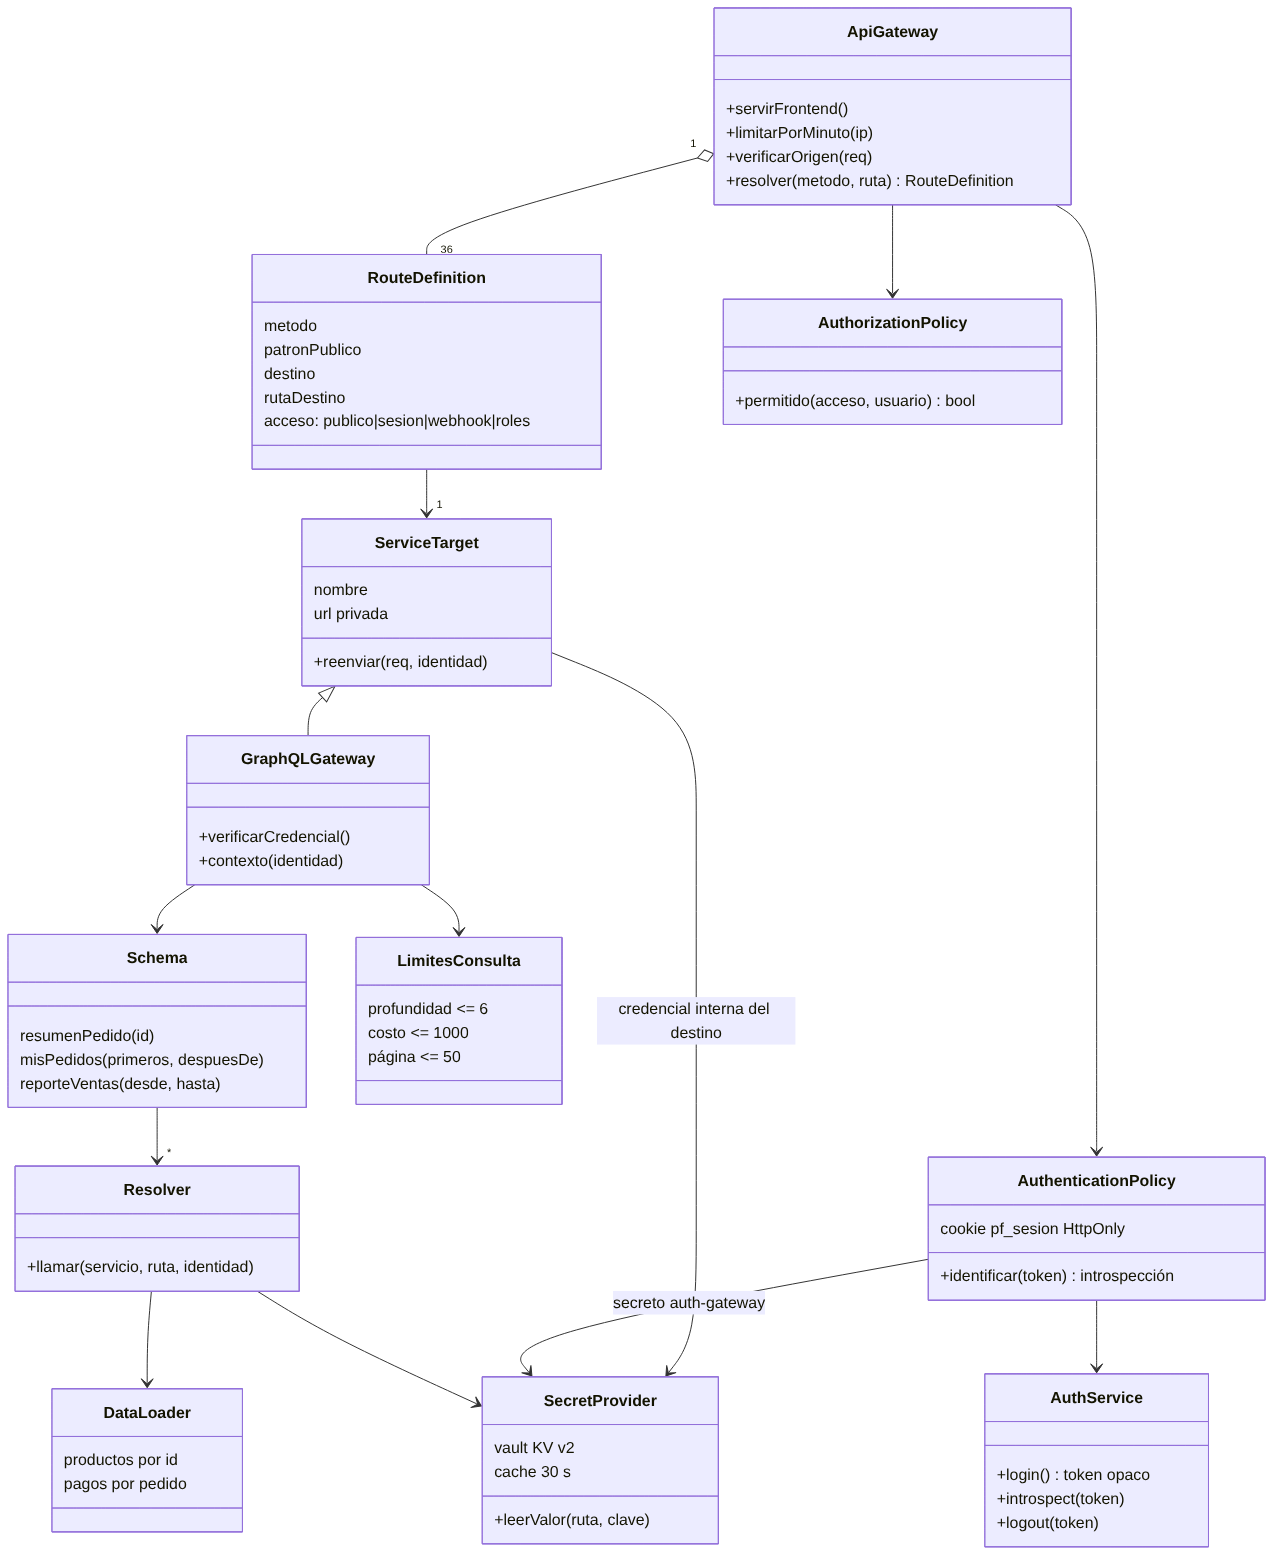
\includegraphics[width=\linewidth,height=0.85\textheight,keepaspectratio]{../diagramas/gateway.png}
\caption{UML del gateway}
\end{figure}

\begin{itemize}[nosep,leftmargin=*]
\item \textbf{RouteDefinition} (\texttt{gateway/\allowbreak{}src/\allowbreak{}rutas.\allowbreak{}js}): 36 filas; lo que no está, responde 404. Las rutas \texttt{/\allowbreak{}internos/\allowbreak{}*} de los servicios nunca se publican.
\item \textbf{AuthenticationPolicy} (\texttt{sesion.\allowbreak{}js}): cookie \texttt{pf\_\allowbreak{}sesion} HttpOnly; introspección en el Auth Service en cada petición.
\item \textbf{AuthorizationPolicy} (\texttt{rutas.\allowbreak{}js:\allowbreak{} permitido}): público, sesión, webhook o lista de roles.
\item \textbf{ServiceTarget} (\texttt{reenvio.\allowbreak{}js}): arma cabeceras nuevas, agrega la credencial del destino y la identidad, reenvía el cuerpo exacto; 502 si no responde, 504 si tarda más de 8~s.
\item \textbf{SecretProvider} (\texttt{vault.\allowbreak{}js}): lee de Vault con el token del gateway, guarda 30~s.
\item \textbf{GraphQLGateway, Schema, Resolver, DataLoader, LimitesConsulta}: en \texttt{graphql-\allowbreak{}gateway/\allowbreak{}} (sección 8).
\item No hay clientes gRPC (ADR 0001).
\end{itemize}

\subsection{Cuántos gateways y por qué}

Hay \textbf{un API Gateway externo} (puerto 8080) y, detrás de él, el \textbf{GraphQL Gateway privado}. No hay un segundo gateway público. Las políticas distintas (anónimo, cliente, personal, webhook) se separan con la columna de acceso de la matriz de rutas, que es lo que pide un solo gateway para separar rutas mediante políticas. Un segundo gateway, por ejemplo solo para el panel administrativo, duplicaría el contenedor, la superficie de ataque y las copias de CSRF, límites y sesión, sin una necesidad concreta: con 44 operaciones y un solo equipo, la ganancia sería nula. El GraphQL Gateway no es un segundo gateway público: es un servicio de agregación sin puerto publicado que hereda la sesión del primero (sección 8).


\subsection{Clasificación de rutas}

{\small
\setlength{\tabcolsep}{3pt}\renewcommand{\arraystretch}{1.15}
\begin{longtable}{|>{\raggedright\arraybackslash}p{\dimexpr 0.2140\linewidth-2\tabcolsep\relax}|>{\raggedright\arraybackslash}p{\dimexpr 0.3930\linewidth-2\tabcolsep\relax}|>{\raggedright\arraybackslash}p{\dimexpr 0.3930\linewidth-2\tabcolsep\relax}|}
\hline
\textbf{Clase} & \textbf{Operaciones} & \textbf{Observación} \\ \hline
\endfirsthead
\hline
\textbf{Clase} & \textbf{Operaciones} & \textbf{Observación} \\ \hline
\endhead
Externas anónimas & 12: S01, S02, S03, S07, S29, S33, S34, S35, S36, S38, S39, S44 & Una ruta pública de red no implica datos públicos: S35 devuelve la sesión si existe y S29 solo acepta una firma válida \\ \hline
Externas autenticadas & 18: S08, S09, S15, S16, S17, S18, S19, S20, S21, S22, S23, S24, S25, S27, S28, S30, S31, S37 & Pueden transportar datos restringidos para un usuario autorizado (sus pedidos, su ficha) \\ \hline
Administrativas (admin o dueño) & 14: S04, S05, S06, S10, S11, S12, S13, S14, S26, S32, S40, S41, S42, S43 & Mantenedores y reportes \\ \hline
Internas (nunca publicadas) & 11 & Inventario: cotizar, reservar y liberar. Clientes: ficha por id. Pedidos: confirmar pago. Pagos: devoluciones y pagos por pedido. Auth: introspección, crear cuenta, cambiar cuenta de un cliente y estado de verificación \\ \hline
\end{longtable}
}

\subsection{Fronteras de confianza}

\begin{figure}[H]
\centering
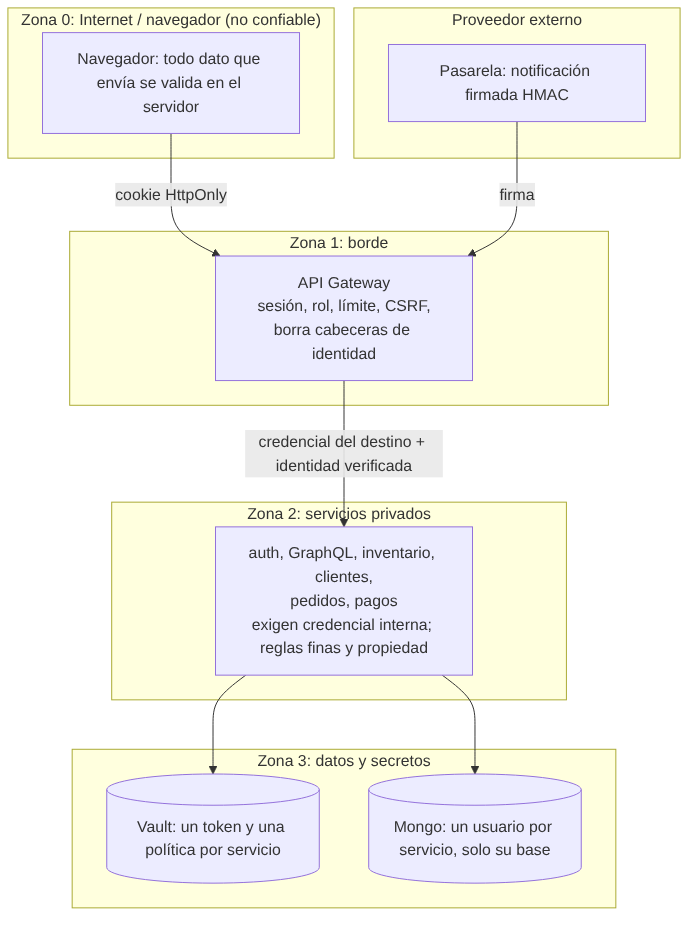
\includegraphics[width=\linewidth,height=0.85\textheight,keepaspectratio]{../diagramas/fronteras.png}
\caption{Fronteras de confianza}
\end{figure}

{\small
\setlength{\tabcolsep}{3pt}\renewcommand{\arraystretch}{1.15}
\begin{longtable}{|>{\raggedright\arraybackslash}p{\dimexpr 0.3149\linewidth-2\tabcolsep\relax}|>{\raggedright\arraybackslash}p{\dimexpr 0.6851\linewidth-2\tabcolsep\relax}|}
\hline
\textbf{Frontera} & \textbf{Qué se verifica al cruzarla} \\ \hline
\endfirsthead
\hline
\textbf{Frontera} & \textbf{Qué se verifica al cruzarla} \\ \hline
\endhead
Navegador $\rightarrow$ gateway & TLS (HTTPS con HSTS), sesión (cookie + introspección), rol, origen (CSRF), límite por IP, tamaño del cuerpo (100~KB). Se descartan \texttt{X-\allowbreak{}Usuario-\allowbreak{}*}, \texttt{X-\allowbreak{}Credencial-\allowbreak{}Interna}, \texttt{Authorization} y la cookie antes de reenviar \\ \hline
Pasarela $\rightarrow$ gateway $\rightarrow$ pagos & Firma HMAC del cuerpo exacto, token y monto \\ \hline
Gateway $\rightarrow$ servicio & Credencial interna del servicio de destino (cada servicio tiene la suya) \\ \hline
Servicio $\rightarrow$ servicio & Credencial del destino + identidad del usuario original (el destino aplica sus reglas) \\ \hline
Servicio $\rightarrow$ Vault & Token propio con política de solo lectura en sus rutas \\ \hline
Servicio $\rightarrow$ Mongo & Usuario propio con \texttt{readWrite} solo en su base, sobre TLS \\ \hline
Todos los saltos & TLS 1.2 o superior: el cliente verifica el certificado del servidor con la CA de prueba (en Node, \texttt{NODE\_\allowbreak{}EXTRA\_\allowbreak{}CA\_\allowbreak{}CERTS}; en Python, \texttt{SSL\_\allowbreak{}CERT\_\allowbreak{}FILE}; en Mongo, \texttt{tlsCAFile}). Un intento en claro contra un servicio interno se rechaza (caso 7.12 y comprobación manual) \\ \hline
\end{longtable}
}

\subsection{Decisiones de separación}

\begin{itemize}[nosep,leftmargin=*]
\item El frontend se sirve desde el gateway: misma origen que la API, la cookie viaja sin CORS y puede ser \texttt{SameSite}.
\item El gateway no tiene reglas de negocio: solo el control grueso. La propiedad del recurso la decide el servicio dueño (así no se puede saltar llamando por GraphQL).
\item El GraphQL Gateway está detrás del API Gateway, no al lado: hereda sesión, límites y CSRF.
\item Pagos es el único servicio privado en la red \texttt{externa}, porque es el único que habla con el proveedor.
\end{itemize}

\subsection{Recorrido de una petición autorizada y una denegada}

\begin{figure}[H]
\centering
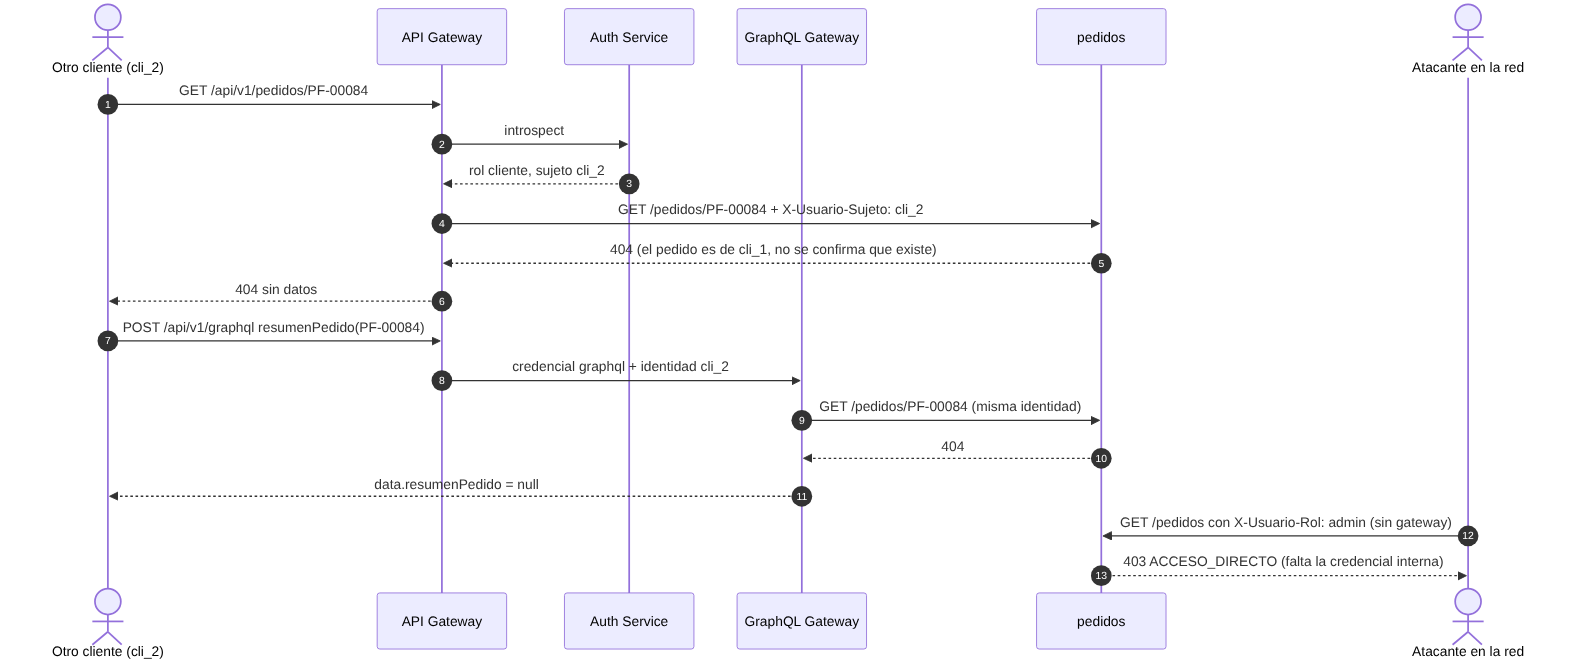
\includegraphics[width=\linewidth,height=0.85\textheight,keepaspectratio]{../diagramas/secuencia-denegada.png}
\caption{Secuencia denegada}
\end{figure}

\textbf{Autorizada:} la cocina acepta el pedido PF-00084. Navegador $\rightarrow$ \texttt{POST /\allowbreak{}api/\allowbreak{}v1/\allowbreak{}pedidos/\allowbreak{}PF-\allowbreak{}00084/\allowbreak{}aceptar} con su cookie $\rightarrow$ el gateway introspecciona (rol \texttt{cocina}) $\rightarrow$ la matriz permite \texttt{admin,\allowbreak{} cocina} $\rightarrow$ lee de Vault la credencial de pedidos $\rightarrow$ reenvía con \texttt{X-\allowbreak{}Usuario-\allowbreak{}Rol:\allowbreak{} cocina} $\rightarrow$ pedidos verifica la credencial, que el rol sea cocina o admin, que el pedido esté PAGADO (en el mismo \texttt{update}) y registra el paso con el nombre de quien lo hizo $\rightarrow$ \texttt{200}. Evidencia: caso 10.4.


\textbf{Denegada:} otro cliente pide el mismo pedido. El gateway lo deja pasar (los clientes pueden ver pedidos), pero pedidos compara \texttt{X-\allowbreak{}Usuario-\allowbreak{}Sujeto} con el dueño y responde 404, sin confirmar que existe. Por GraphQL ocurre lo mismo, porque el GraphQL Gateway reenvía la identidad. Si alguien en la red privada llama directo a pedidos con \texttt{X-\allowbreak{}Usuario-\allowbreak{}Rol:\allowbreak{} admin}, recibe 403 por no tener la credencial interna. Evidencia: casos 7.5 y 7.9.


\clearpage
% Generado desde docs/INFORME.md. Editar libremente.

\section{6. Rutas, secretos, identidades y operaciones GraphQL}

Cada petición que llega de afuera debe terminar en el servicio correcto, y cada servicio necesita una forma de demostrar quién es. Aquí está el mapa completo: qué ruta pública va a qué servicio, con qué control y con qué credencial; qué secretos existen, quién los usa y cómo se cambian; y qué operaciones ofrece GraphQL. Las credenciales se nombran por su ubicación en Vault, nunca por su valor.


\subsection{Cómo se piensan las llaves}

La imagen que sirve aquí es la de un edificio con muchas puertas. Cada servicio tiene su propia llave y esa llave no abre las demás: si alguien consigue la de pagos, solo entra a pagos. El gateway es el único que lleva varias llaves, porque su trabajo es llamar a todos, y por eso es la pieza más vigilada. Los tres tipos de identidad que aparecen en esta sección son distintos entre sí: la \textbf{persona} se identifica con su cookie de sesión, un \textbf{servicio} con su credencial interna, y la \textbf{pasarela} con la firma de sus avisos.


Las llaves no están escritas en el código ni en el repositorio: viven en Vault, y \texttt{vault-\allowbreak{}init}, el contenedor que corre una sola vez al arrancar, las crea al azar. Cada servicio recibe un token que solo le permite leer sus propias rutas, y cada uno tiene su propio usuario de base de datos. Una limitación que está declarada entre las brechas de la sección 0: en Docker Compose los tokens de todos los servicios se escriben en un mismo volumen de solo lectura, en vez de montarse cada uno solo en su contenedor; lo que protege es que cada token solo puede leer sus propias rutas de Vault. En producción lo resolvería el orquestador (Docker secrets o Kubernetes). Si Vault deja de responder, el sistema se cierra en vez de abrirse: después de unos minutos de gracia, los servicios responden 503 y no dejan pasar a nadie.


\subsection{Matriz de rutas}

Cada fila es una operación del módulo 1 (mismo ID). Lo que no está en esta tabla no existe hacia afuera (404). Las rutas \texttt{/\allowbreak{}internos/\allowbreak{}*} de los servicios nunca se publican. Se generó leyendo \texttt{gateway/\allowbreak{}src/\allowbreak{}rutas.\allowbreak{}js}, que tiene 36 filas (S30 a S32 comparten la de \texttt{/\allowbreak{}graphql}); a ellas se suman 6 operaciones que resuelve el propio gateway (S33 a S37 y S44). Controles que se aplican a \textbf{todas} las rutas, además de los de la columna: HTTPS con HSTS, límite general por IP, origen permitido en los verbos que cambian datos (CSRF), cuerpo de hasta 100~KB, plazo de 8~s (504 si se vence, 502 si el servicio no responde), errores con la misma forma y \texttt{X-\allowbreak{}Request-\allowbreak{}Id} en los logs. Antes de reenviar, el gateway descarta \texttt{X-\allowbreak{}Usuario-\allowbreak{}*}, \texttt{X-\allowbreak{}Credencial-\allowbreak{}Interna}, \texttt{Authorization} y la cookie, y agrega solo la identidad verificada y la credencial del destino.


\begin{landscape}
\vspace{0.6em}
{\scriptsize
\setlength{\LTpre}{0pt}\setlength{\LTpost}{0pt}
\setlength{\tabcolsep}{3pt}\renewcommand{\arraystretch}{1.15}
\begin{longtable}{|>{\raggedright\arraybackslash}p{\dimexpr 0.0455\linewidth-2\tabcolsep\relax}|>{\raggedright\arraybackslash}p{\dimexpr 0.0711\linewidth-2\tabcolsep\relax}|>{\raggedright\arraybackslash}p{\dimexpr 0.0775\linewidth-2\tabcolsep\relax}|>{\raggedright\arraybackslash}p{\dimexpr 0.1278\linewidth-2\tabcolsep\relax}|>{\raggedright\arraybackslash}p{\dimexpr 0.1077\linewidth-2\tabcolsep\relax}|>{\raggedright\arraybackslash}p{\dimexpr 0.1745\linewidth-2\tabcolsep\relax}|>{\raggedright\arraybackslash}p{\dimexpr 0.2008\linewidth-2\tabcolsep\relax}|>{\raggedright\arraybackslash}p{\dimexpr 0.1950\linewidth-2\tabcolsep\relax}|}
\hline
\textbf{ID} & \textbf{Gateway} & \textbf{Verbo} & \textbf{Ruta externa (\texttt{/\allowbreak{}api/\allowbreak{}v1})} & \textbf{Acceso y rol} & \textbf{Sistema y ruta destino} & \textbf{Controles propios} & \textbf{Referencia de credencial} \\ \hline
\endfirsthead
\hline
\textbf{ID} & \textbf{Gateway} & \textbf{Verbo} & \textbf{Ruta externa (\texttt{/\allowbreak{}api/\allowbreak{}v1})} & \textbf{Acceso y rol} & \textbf{Sistema y ruta destino} & \textbf{Controles propios} & \textbf{Referencia de credencial} \\ \hline
\endhead
S01 & gateway externo & GET & \texttt{/\allowbreak{}catalogo/\allowbreak{}items} & Público & inventario: \texttt{/\allowbreak{}items} & Filtros validados (400) & \texttt{internos/\allowbreak{}inventario} \\ \hline
S02 & gateway externo & GET & \texttt{/\allowbreak{}catalogo/\allowbreak{}items/\allowbreak{}:\allowbreak{}id} & Público & inventario: \texttt{/\allowbreak{}items/\allowbreak{}:\allowbreak{}id} & — & \texttt{internos/\allowbreak{}inventario} \\ \hline
S03 & gateway externo & GET & \texttt{/\allowbreak{}catalogo/\allowbreak{}configuracion} & Público & inventario: \texttt{/\allowbreak{}configuracion} & — & \texttt{internos/\allowbreak{}inventario} \\ \hline
S04 & gateway externo & POST & \texttt{/\allowbreak{}catalogo/\allowbreak{}items} & admin, dueño & inventario: \texttt{/\allowbreak{}items} & Validación de producto & \texttt{internos/\allowbreak{}inventario} \\ \hline
S05 & gateway externo & PUT & \texttt{/\allowbreak{}catalogo/\allowbreak{}items/\allowbreak{}:\allowbreak{}id} & admin, dueño & inventario: \texttt{/\allowbreak{}items/\allowbreak{}:\allowbreak{}id} & Validación de producto & \texttt{internos/\allowbreak{}inventario} \\ \hline
S06 & gateway externo & DELETE & \texttt{/\allowbreak{}catalogo/\allowbreak{}items/\allowbreak{}:\allowbreak{}id} & admin & inventario: \texttt{/\allowbreak{}items/\allowbreak{}:\allowbreak{}id} & Solo admin en gateway e inventario & \texttt{internos/\allowbreak{}inventario} \\ \hline
S07 & gateway externo & POST & \texttt{/\allowbreak{}clientes/\allowbreak{}registro} & Público & clientes: \texttt{/\allowbreak{}clientes/\allowbreak{}registro} & 20/min por IP; validación de ficha & \texttt{internos/\allowbreak{}clientes} \\ \hline
S08 & gateway externo & GET & \texttt{/\allowbreak{}clientes/\allowbreak{}yo} & cliente & clientes: \texttt{/\allowbreak{}clientes/\allowbreak{}yo} & Propiedad & \texttt{internos/\allowbreak{}clientes} \\ \hline
S09 & gateway externo & PUT & \texttt{/\allowbreak{}clientes/\allowbreak{}yo} & cliente & clientes: \texttt{/\allowbreak{}clientes/\allowbreak{}yo} & Propiedad & \texttt{internos/\allowbreak{}clientes} \\ \hline
S10 & gateway externo & GET & \texttt{/\allowbreak{}clientes} & admin & clientes: \texttt{/\allowbreak{}clientes} & — & \texttt{internos/\allowbreak{}clientes} \\ \hline
S11 & gateway externo & POST & \texttt{/\allowbreak{}clientes} & admin & clientes: \texttt{/\allowbreak{}clientes} & Clave temporal & \texttt{internos/\allowbreak{}clientes} \\ \hline
S12 & gateway externo & GET & \texttt{/\allowbreak{}clientes/\allowbreak{}:\allowbreak{}id} & admin & clientes: \texttt{/\allowbreak{}clientes/\allowbreak{}:\allowbreak{}id} & — & \texttt{internos/\allowbreak{}clientes} \\ \hline
S13 & gateway externo & PUT & \texttt{/\allowbreak{}clientes/\allowbreak{}:\allowbreak{}id} & admin & clientes: \texttt{/\allowbreak{}clientes/\allowbreak{}:\allowbreak{}id} & — & \texttt{internos/\allowbreak{}clientes} \\ \hline
S14 & gateway externo & PATCH & \texttt{/\allowbreak{}clientes/\allowbreak{}:\allowbreak{}id/\allowbreak{}estado} & admin & clientes: \texttt{/\allowbreak{}clientes/\allowbreak{}:\allowbreak{}id/\allowbreak{}estado} & Cierra sesiones al desactivar & \texttt{internos/\allowbreak{}clientes} \\ \hline
S15 & gateway externo & POST & \texttt{/\allowbreak{}pedidos} & cliente & pedidos: \texttt{/\allowbreak{}pedidos} & \texttt{Idempotency-\allowbreak{}Key}; precio de inventario & \texttt{internos/\allowbreak{}pedidos} \\ \hline
S16 & gateway externo & GET & \texttt{/\allowbreak{}pedidos} & Todos los roles & pedidos: \texttt{/\allowbreak{}pedidos} & Propiedad y filtro por rol & \texttt{internos/\allowbreak{}pedidos} \\ \hline
S17 & gateway externo & GET & \texttt{/\allowbreak{}pedidos/\allowbreak{}:\allowbreak{}id} & Todos los roles & pedidos: \texttt{/\allowbreak{}pedidos/\allowbreak{}:\allowbreak{}id} & Propiedad y filtro por rol & \texttt{internos/\allowbreak{}pedidos} \\ \hline
S18 & gateway externo & GET & \texttt{/\allowbreak{}pedidos/\allowbreak{}boleta/\allowbreak{}:\allowbreak{}numero} & cliente, admin, dueño & pedidos: \texttt{/\allowbreak{}pedidos/\allowbreak{}boleta/\allowbreak{}:\allowbreak{}numero} & Propiedad & \texttt{internos/\allowbreak{}pedidos} \\ \hline
S19 & gateway externo & GET & \texttt{/\allowbreak{}pedidos/\allowbreak{}configuracion} & Todos los roles & pedidos: \texttt{/\allowbreak{}pedidos-\allowbreak{}config} & — & \texttt{internos/\allowbreak{}pedidos} \\ \hline
S20 & gateway externo & POST & \texttt{/\allowbreak{}pedidos/\allowbreak{}:\allowbreak{}id/\allowbreak{}aceptar} & admin, cocina & pedidos: \texttt{/\allowbreak{}pedidos/\allowbreak{}:\allowbreak{}id/\allowbreak{}aceptar} & Estado atómico & \texttt{internos/\allowbreak{}pedidos} \\ \hline
S21 & gateway externo & POST & \texttt{/\allowbreak{}pedidos/\allowbreak{}:\allowbreak{}id/\allowbreak{}terminar} & admin, cocina & pedidos: \texttt{/\allowbreak{}pedidos/\allowbreak{}:\allowbreak{}id/\allowbreak{}terminar} & Estado atómico & \texttt{internos/\allowbreak{}pedidos} \\ \hline
S22 & gateway externo & POST & \texttt{/\allowbreak{}pedidos/\allowbreak{}:\allowbreak{}id/\allowbreak{}despachar} & admin, despacho & pedidos: \texttt{/\allowbreak{}pedidos/\allowbreak{}:\allowbreak{}id/\allowbreak{}despachar} & Estado atómico & \texttt{internos/\allowbreak{}pedidos} \\ \hline
S23 & gateway externo & POST & \texttt{/\allowbreak{}pedidos/\allowbreak{}:\allowbreak{}id/\allowbreak{}entregar} & admin, despacho & pedidos: \texttt{/\allowbreak{}pedidos/\allowbreak{}:\allowbreak{}id/\allowbreak{}entregar} & Estado atómico & \texttt{internos/\allowbreak{}pedidos} \\ \hline
S24 & gateway externo & POST & \texttt{/\allowbreak{}pedidos/\allowbreak{}:\allowbreak{}id/\allowbreak{}impresa} & admin, cocina, despacho & pedidos: \texttt{/\allowbreak{}pedidos/\allowbreak{}:\allowbreak{}id/\allowbreak{}impresa} & — & \texttt{internos/\allowbreak{}pedidos} \\ \hline
S25 & gateway externo & POST & \texttt{/\allowbreak{}pedidos/\allowbreak{}:\allowbreak{}id/\allowbreak{}anular} & cliente, admin & pedidos: \texttt{/\allowbreak{}pedidos/\allowbreak{}:\allowbreak{}id/\allowbreak{}anular} & Propiedad, estado y motivo & \texttt{internos/\allowbreak{}pedidos} \\ \hline
S26 & gateway externo & GET & \texttt{/\allowbreak{}reportes/\allowbreak{}ventas} & admin, dueño & pedidos: \texttt{/\allowbreak{}reportes/\allowbreak{}ventas} & Período $\leq$ 1 año & \texttt{internos/\allowbreak{}pedidos} \\ \hline
S27 & gateway externo & POST & \texttt{/\allowbreak{}pagos} & cliente & pagos: \texttt{/\allowbreak{}pagos} & \texttt{Idempotency-\allowbreak{}Key} obligatoria; propiedad vía pedidos & \texttt{internos/\allowbreak{}pagos} \\ \hline
S28 & gateway externo & GET & \texttt{/\allowbreak{}pagos} & cliente, admin, dueño & pagos: \texttt{/\allowbreak{}pagos} & Propiedad vía pedidos & \texttt{internos/\allowbreak{}pagos} \\ \hline
S29 & gateway externo & POST & \texttt{/\allowbreak{}pagos/\allowbreak{}notificacion} & Sin sesión (firma de la pasarela) & pagos: \texttt{/\allowbreak{}pagos/\allowbreak{}notificacion} & Firma HMAC; se reenvía sin identidad de usuario & \texttt{internos/\allowbreak{}pagos}; firma con \texttt{pasarela/\allowbreak{}comercio} (\texttt{secreto\_\allowbreak{}firma}) \\ \hline
S30 & gateway externo & POST & \texttt{/\allowbreak{}graphql} \texttt{resumenPedido} & Con sesión & GraphQL Gateway: \texttt{/\allowbreak{}graphql} & Profundidad $\leq$ 6, costo $\leq$ 1.000, paginación $\leq$ 50 & \texttt{internos/\allowbreak{}graphql} \\ \hline
S31 & gateway externo & POST & \texttt{/\allowbreak{}graphql} \texttt{misPedidos} & Con sesión & GraphQL Gateway: \texttt{/\allowbreak{}graphql} & Profundidad, costo y paginación & \texttt{internos/\allowbreak{}graphql} \\ \hline
S32 & gateway externo & POST & \texttt{/\allowbreak{}graphql} \texttt{reporteVentas} & Con sesión & GraphQL Gateway: \texttt{/\allowbreak{}graphql} & Profundidad, costo y paginación & \texttt{internos/\allowbreak{}graphql} \\ \hline
S33 & gateway externo & POST & \texttt{/\allowbreak{}auth/\allowbreak{}login} & Público & Auth Service: \texttt{/\allowbreak{}login} & 20/min por IP; bloqueo por correo & \texttt{internos/\allowbreak{}auth-\allowbreak{}gateway} (Basic) \\ \hline
S34 & gateway externo & POST & \texttt{/\allowbreak{}auth/\allowbreak{}logout} & Público & Auth Service: \texttt{/\allowbreak{}logout} & Borra la cookie & \texttt{internos/\allowbreak{}auth-\allowbreak{}gateway} (Basic) \\ \hline
S35 & gateway externo & GET & \texttt{/\allowbreak{}auth/\allowbreak{}sesion} & Público & gateway (no reenvía) & Respuesta del propio gateway & — \\ \hline
S36 & gateway externo & GET & \texttt{/\allowbreak{}auth/\allowbreak{}config} & Público & gateway (no reenvía) & Respuesta del propio gateway & — \\ \hline
S37 & gateway externo & PUT & \texttt{/\allowbreak{}auth/\allowbreak{}clave} & Con sesión & Auth Service: \texttt{/\allowbreak{}clave} & Cuenta tomada de la sesión & \texttt{internos/\allowbreak{}auth-\allowbreak{}gateway} (Basic) \\ \hline
S38 & gateway externo & POST & \texttt{/\allowbreak{}auth/\allowbreak{}verificar} & Público & Auth Service: \texttt{/\allowbreak{}verificacion} & 20/min por IP; respuesta uniforme & \texttt{internos/\allowbreak{}auth-\allowbreak{}gateway} (Basic) \\ \hline
S39 & gateway externo & POST & \texttt{/\allowbreak{}auth/\allowbreak{}reenviar} & Público & Auth Service: \texttt{/\allowbreak{}verificacion/\allowbreak{}reenviar} & 20/min por IP; respuesta uniforme & \texttt{internos/\allowbreak{}auth-\allowbreak{}gateway} (Basic) \\ \hline
S40 & gateway externo & GET & \texttt{/\allowbreak{}usuarios} & admin & Auth Service: \texttt{/\allowbreak{}usuarios} & — & \texttt{internos/\allowbreak{}auth-\allowbreak{}gateway} (Basic) \\ \hline
S41 & gateway externo & POST & \texttt{/\allowbreak{}usuarios} & admin & Auth Service: \texttt{/\allowbreak{}usuarios} & Clave fuerte & \texttt{internos/\allowbreak{}auth-\allowbreak{}gateway} (Basic) \\ \hline
S42 & gateway externo & PUT & \texttt{/\allowbreak{}usuarios/\allowbreak{}:\allowbreak{}id} & admin & Auth Service: \texttt{/\allowbreak{}usuarios/\allowbreak{}:\allowbreak{}id} & Último admin y propio perfil protegidos & \texttt{internos/\allowbreak{}auth-\allowbreak{}gateway} (Basic) \\ \hline
S43 & gateway externo & PATCH & \texttt{/\allowbreak{}usuarios/\allowbreak{}:\allowbreak{}id/\allowbreak{}estado} & admin & Auth Service: \texttt{/\allowbreak{}usuarios/\allowbreak{}:\allowbreak{}id/\allowbreak{}estado} & Último admin y propia cuenta protegidos & \texttt{internos/\allowbreak{}auth-\allowbreak{}gateway} (Basic) \\ \hline
S44 & gateway externo & GET & \texttt{/\allowbreak{}api/\allowbreak{}salud} & Público & gateway: \texttt{GET /\allowbreak{}salud} de cada servicio y de Vault & Sin datos personales; consulta cada \texttt{/\allowbreak{}salud} con 2~s de plazo & — \\ \hline
\end{longtable}
}
\end{landscape}

\begin{landscape}
Las referencias de credencial son rutas simbólicas en Vault (\texttt{secret/\allowbreak{}poke-\allowbreak{}fresh/\allowbreak{}.\allowbreak{}.\allowbreak{}.\allowbreak{}}), no valores. Los tres GraphQL (S30 a S32) comparten la ruta \texttt{POST /\allowbreak{}graphql}: el gateway solo exige sesión y \textbf{cada operación y cada campo se autoriza dentro del GraphQL Gateway} (tabla de la sección 8); que la ruta esté permitida no autoriza todas sus operaciones.

\subsection{Inventario simbólico de secretos}
Referencias, nunca valores. Todos los genera \texttt{vault-\allowbreak{}init} al azar (256 bits) y viven en Vault (\texttt{secret/\allowbreak{}}, KV v2), salvo \texttt{MONGO\_\allowbreak{}ROOT\_\allowbreak{}CLAVE}. Ninguno está en el repositorio, en el JavaScript del navegador, en capturas ni en logs. Cada servicio lee solo los suyos: su token de Vault tiene una política de solo lectura sobre esas rutas.

\vspace{0.6em}
{\scriptsize
\setlength{\LTpre}{0pt}\setlength{\LTpost}{0pt}
\setlength{\tabcolsep}{3pt}\renewcommand{\arraystretch}{1.15}
\begin{longtable}{|>{\raggedright\arraybackslash}p{\dimexpr 0.1393\linewidth-2\tabcolsep\relax}|>{\raggedright\arraybackslash}p{\dimexpr 0.0928\linewidth-2\tabcolsep\relax}|>{\raggedright\arraybackslash}p{\dimexpr 0.1184\linewidth-2\tabcolsep\relax}|>{\raggedright\arraybackslash}p{\dimexpr 0.0926\linewidth-2\tabcolsep\relax}|>{\raggedright\arraybackslash}p{\dimexpr 0.1295\linewidth-2\tabcolsep\relax}|>{\raggedright\arraybackslash}p{\dimexpr 0.1483\linewidth-2\tabcolsep\relax}|>{\raggedright\arraybackslash}p{\dimexpr 0.1309\linewidth-2\tabcolsep\relax}|>{\raggedright\arraybackslash}p{\dimexpr 0.1483\linewidth-2\tabcolsep\relax}|}
\hline
\textbf{Referencia} & \textbf{Tipo} & \textbf{Emisor} & \textbf{Consumidor (política)} & \textbf{Finalidad} & \textbf{Ubicación segura} & \textbf{Alcance} & \textbf{Rotación y revocación} \\ \hline
\endfirsthead
\hline
\textbf{Referencia} & \textbf{Tipo} & \textbf{Emisor} & \textbf{Consumidor (política)} & \textbf{Finalidad} & \textbf{Ubicación segura} & \textbf{Alcance} & \textbf{Rotación y revocación} \\ \hline
\endhead
\texttt{poke-\allowbreak{}fresh/\allowbreak{}internos/\allowbreak{}inventario} (\texttt{credencial}) & Credencial de servicio & \texttt{vault-\allowbreak{}init} & gateway, inventario, pedidos, graphql & Llamar a inventario & Vault & Solo inventario & Borrar el secreto y volver a correr \texttt{vault-\allowbreak{}init}; los servicios lo leen en $\leq$ 30~s \\ \hline
\texttt{poke-\allowbreak{}fresh/\allowbreak{}internos/\allowbreak{}clientes} (\texttt{credencial}) & Credencial de servicio & \texttt{vault-\allowbreak{}init} & gateway, clientes, pedidos, graphql & Llamar a clientes & Vault & Solo clientes & Igual \\ \hline
\texttt{poke-\allowbreak{}fresh/\allowbreak{}internos/\allowbreak{}pedidos} (\texttt{credencial}) & Credencial de servicio & \texttt{vault-\allowbreak{}init} & gateway, pedidos, pagos, graphql & Llamar a pedidos & Vault & Solo pedidos & Igual \\ \hline
\texttt{poke-\allowbreak{}fresh/\allowbreak{}internos/\allowbreak{}pagos} (\texttt{credencial}) & Credencial de servicio & \texttt{vault-\allowbreak{}init} & gateway, pagos, pedidos, graphql & Llamar a pagos & Vault & Solo pagos & Igual \\ \hline
\texttt{poke-\allowbreak{}fresh/\allowbreak{}internos/\allowbreak{}graphql} (\texttt{credencial}) & Credencial de servicio & \texttt{vault-\allowbreak{}init} & gateway, graphql & Llamar al GraphQL Gateway & Vault & Solo graphql & Igual \\ \hline
\texttt{poke-\allowbreak{}fresh/\allowbreak{}internos/\allowbreak{}auth-\allowbreak{}gateway} (\texttt{secreto}) & Secreto compartido (Basic) & \texttt{vault-\allowbreak{}init} & gateway, auth & El gateway ante el Auth Service & Vault & Rutas de sesión y usuarios del Auth Service & Rotar: el gateway lo relee en $\leq$ 30~s \\ \hline
\texttt{poke-\allowbreak{}fresh/\allowbreak{}internos/\allowbreak{}auth-\allowbreak{}clientes} (\texttt{secreto}) & Secreto compartido (Basic) & \texttt{vault-\allowbreak{}init} & clientes, auth & El servicio de clientes ante el Auth Service & Vault & Solo \texttt{/\allowbreak{}cuentas} (crear y cambiar cuentas de cliente) & Rotar \\ \hline
\texttt{poke-\allowbreak{}fresh/\allowbreak{}auth} (\texttt{pepper}) & Pepper de contraseñas & \texttt{vault-\allowbreak{}init} (una sola vez) & auth & Se mezcla con la clave antes de scrypt & Vault & Hashes de contraseñas & \textbf{No se rota a la ligera}: obliga a pedir cambio de contraseña a todos. Por eso \texttt{vault-\allowbreak{}init} nunca lo regenera \\ \hline
\texttt{poke-\allowbreak{}fresh/\allowbreak{}pasarela/\allowbreak{}comercio} (\texttt{api\_\allowbreak{}key}, \texttt{secreto\_\allowbreak{}firma}) & Claves del comercio ante el proveedor & \texttt{vault-\allowbreak{}init} en la demostración; el proveedor en producción & pagos, pasarela & Crear transacciones y firmar o verificar notificaciones & Vault & Operar la cuenta del comercio (nunca llega al navegador) & Pedir claves nuevas al proveedor y actualizar el secreto \\ \hline
\texttt{poke-\allowbreak{}fresh/\allowbreak{}mongo/\allowbreak{}<servicio>} (\texttt{usuario}, \texttt{clave}) & Credencial de base de datos & \texttt{vault-\allowbreak{}init} & ese servicio (y \texttt{semilla} la suya) & Conectarse a su base & Vault & \texttt{readWrite} solo en su base & Cambiar la clave en Vault y correr \texttt{vault-\allowbreak{}init} (actualiza el usuario en Mongo) \\ \hline
Token de Vault de cada servicio & Token con TTL 720 h & Vault, vía \texttt{vault-\allowbreak{}init} & ese servicio & Leer sus rutas & Volumen de solo lectura (ver «Distribución de tokens de Vault» en las brechas de la sección 0) & Solo lectura de sus rutas & Revocarlo en Vault; \texttt{vault-\allowbreak{}init} emite uno nuevo \\ \hline
\texttt{MONGO\_\allowbreak{}ROOT\_\allowbreak{}CLAVE} & Secreto de arranque & La persona que opera & mongo, vault-init & Crear los usuarios por servicio & \texttt{.\allowbreak{}env} fuera del repo & Administrar Mongo (ningún servicio la usa) & Cambiarla en Mongo y en \texttt{.\allowbreak{}env} \\ \hline
Certificados TLS y CA de prueba & Certificados & \texttt{tls-\allowbreak{}init} & todos los servicios & Cifrar y autenticar cada salto & Volúmenes \texttt{tls} (certificados) y \texttt{tls-\allowbreak{}ca} (clave de la CA, solo \texttt{tls-\allowbreak{}init}) & Un certificado por componente & Borrar el volumen \texttt{tls} y recrear: se emiten nuevos \\ \hline
\end{longtable}
}
\end{landscape}

\textbf{Si una clave se filtra:} se revoca o borra el secreto afectado y se corre \texttt{vault-\allowbreak{}init}; solo se ve comprometido lo que esa referencia permite (la columna Alcance), porque no hay un secreto común a todos los sistemas. Una credencial de pagos solo sirve para pagos; la de base de datos de un servicio no abre las de otro; el navegador nunca recibe ninguna.


\textbf{Si Vault no responde:} cada servicio sigue usando lo leído durante 5 minutos (\texttt{VAULT\_\allowbreak{}GRACIA\_\allowbreak{}SEGUNDOS}) y después responde 503 (falla cerrada). El gateway responde 503 \texttt{SECRETOS\_\allowbreak{}NO\_\allowbreak{}DISPONIBLES}. Probado en el caso 10.7.


\subsection{Identidades}

{\small
\setlength{\tabcolsep}{3pt}\renewcommand{\arraystretch}{1.15}
\begin{longtable}{|>{\raggedright\arraybackslash}p{\dimexpr 0.2485\linewidth-2\tabcolsep\relax}|>{\raggedright\arraybackslash}p{\dimexpr 0.4191\linewidth-2\tabcolsep\relax}|>{\raggedright\arraybackslash}p{\dimexpr 0.3323\linewidth-2\tabcolsep\relax}|}
\hline
\textbf{Identidad} & \textbf{Cómo se prueba} & \textbf{Dónde se valida} \\ \hline
\endfirsthead
\hline
\textbf{Identidad} & \textbf{Cómo se prueba} & \textbf{Dónde se valida} \\ \hline
\endhead
Usuario (cliente o personal) & Cookie con token opaco & Auth Service (introspección), por el gateway \\ \hline
Gateway ante servicios & \texttt{X-\allowbreak{}Credencial-\allowbreak{}Interna} del destino & Cada servicio, contra Vault \\ \hline
Gateway / clientes ante Auth & HTTP Basic (sobre HTTPS) con su secreto & Auth Service, contra Vault, y solo sus rutas \\ \hline
Servicio ante otro servicio & Credencial del destino + identidad del usuario original & El destino \\ \hline
Pasarela ante pagos & Firma HMAC del cuerpo & pagos \\ \hline
Pagos ante la pasarela & \texttt{X-\allowbreak{}Api-\allowbreak{}Key} & pasarela \\ \hline
Servicio ante Vault & Token con política propia & Vault \\ \hline
Servicio ante Mongo & Usuario y clave propios & Mongo (\texttt{authSource} = su base) \\ \hline
\end{longtable}
}

\subsection{Operaciones GraphQL}

{\footnotesize
\setlength{\tabcolsep}{3pt}\renewcommand{\arraystretch}{1.15}
\begin{longtable}{|>{\raggedright\arraybackslash}p{\dimexpr 0.2191\linewidth-2\tabcolsep\relax}|>{\raggedright\arraybackslash}p{\dimexpr 0.0956\linewidth-2\tabcolsep\relax}|>{\raggedright\arraybackslash}p{\dimexpr 0.1674\linewidth-2\tabcolsep\relax}|>{\raggedright\arraybackslash}p{\dimexpr 0.3188\linewidth-2\tabcolsep\relax}|>{\raggedright\arraybackslash}p{\dimexpr 0.1991\linewidth-2\tabcolsep\relax}|}
\hline
\textbf{Operación} & \textbf{Tipo} & \textbf{Quién} & \textbf{Servicios que combina} & \textbf{Pantalla} \\ \hline
\endfirsthead
\hline
\textbf{Operación} & \textbf{Tipo} & \textbf{Quién} & \textbf{Servicios que combina} & \textbf{Pantalla} \\ \hline
\endhead
\texttt{resumenPedido(\allowbreak{}id)} & query & dueño del pedido y personal & pedidos, pagos, inventario (+ clientes para admin) & \texttt{\#/\allowbreak{}orden/\allowbreak{}:\allowbreak{}id} \\ \hline
\texttt{misPedidos(\allowbreak{}primeros,\allowbreak{} despuesDe)} & query & cliente & pedidos & (disponible; la lista usa REST) \\ \hline
\texttt{reporteVentas(\allowbreak{}desde,\allowbreak{} hasta)} & query & admin, dueño & pedidos, inventario, pagos & \texttt{\#/\allowbreak{}admin/\allowbreak{}reportes} \\ \hline
\end{longtable}
}

No hay mutaciones en GraphQL: los cambios van por REST al servicio dueño, que aplica las reglas transaccionales.


\subsection{Métodos gRPC}

No aplica: no se implementó gRPC. La justificación, con los argumentos a favor y en contra y la evaluación de cada flujo, está en la sección 9 (“gRPC: por qué sí y por qué no”) y en el ADR 0001 (\texttt{docs/\allowbreak{}adr/\allowbreak{}0001-\allowbreak{}analitica-\allowbreak{}y-\allowbreak{}grpc.\allowbreak{}md}).


\clearpage
% Generado desde README.md. Editar libremente.

\begin{landscape}
\section{7. Datos sensibles y secretos del cliente}
No todos los datos valen lo mismo: el nombre de un bowl es público, pero el RUN, la dirección o el historial de pedidos de Javiera no lo son. Esta sección clasifica cada dato, decide quién puede verlo y cómo se protege, aclara que el sistema no guarda secretos de los clientes (ni datos de tarjeta) y termina con las pruebas que se ejecutaron contra el sistema funcionando.

\subsection{Clasificación de datos}
\vspace{0.6em}
{\scriptsize
\setlength{\LTpre}{0pt}\setlength{\LTpost}{0pt}
\setlength{\tabcolsep}{3pt}\renewcommand{\arraystretch}{1.15}
\begin{longtable}{|>{\raggedright\arraybackslash}p{\dimexpr 0.1441\linewidth-2\tabcolsep\relax}|>{\raggedright\arraybackslash}p{\dimexpr 0.1129\linewidth-2\tabcolsep\relax}|>{\raggedright\arraybackslash}p{\dimexpr 0.1061\linewidth-2\tabcolsep\relax}|>{\raggedright\arraybackslash}p{\dimexpr 0.0863\linewidth-2\tabcolsep\relax}|>{\raggedright\arraybackslash}p{\dimexpr 0.1239\linewidth-2\tabcolsep\relax}|>{\raggedright\arraybackslash}p{\dimexpr 0.0880\linewidth-2\tabcolsep\relax}|>{\raggedright\arraybackslash}p{\dimexpr 0.1706\linewidth-2\tabcolsep\relax}|>{\raggedright\arraybackslash}p{\dimexpr 0.1681\linewidth-2\tabcolsep\relax}|}
\hline
\textbf{Dato o credencial} & \textbf{Finalidad} & \textbf{Clasificación} & \textbf{Sistema custodio} & \textbf{Roles autorizados} & \textbf{En el frontend} & \textbf{Protección} & \textbf{Retención} \\ \hline
\endfirsthead
\hline
\textbf{Dato o credencial} & \textbf{Finalidad} & \textbf{Clasificación} & \textbf{Sistema custodio} & \textbf{Roles autorizados} & \textbf{En el frontend} & \textbf{Protección} & \textbf{Retención} \\ \hline
\endhead
Nombre, descripción, precio de productos & Vender & Público & inventario & Todos; editar admin/dueño & Menú & Validación en servidor & Mientras exista el producto \\ \hline
Stock & Evitar sobreventa & Interno & inventario & admin, dueño & Solo panel & DTO por rol & Siempre actualizado \\ \hline
RUN & Boleta e identificación del comprador (caso) & Personal & clientes (y copia en el pedido) & El cliente, admin, dueño & Mis datos, boleta & No sale a cocina ni despacho; no va en logs & Mientras la cuenta exista; en la boleta, lo que exija la ley tributaria \\ \hline
Nombre y teléfono & Contacto y entrega & Personal & clientes (copia en el pedido) & Cliente, personal & Panel, orden & Mínimo necesario & Igual \\ \hline
Dirección y comuna & Despacho & Personal & clientes (copia si es despacho) & Cliente, admin, cocina y despacho en el pedido & Orden de despacho & No va en el catálogo ni en logs & Igual \\ \hline
Correo & Cuenta, boleta & Personal & clientes y Auth & Cliente, admin & Mis datos & No va en logs (el notificador registra solo el dominio) & Igual \\ \hline
Fecha de nacimiento, sexo & Requeridos por el caso para el registro & Personal & clientes & Cliente, admin & Mis datos & Nunca salen en pedidos & Igual \\ \hline
Contraseña & Autenticar & Credencial & Auth (solo el hash) & Nadie la ve & Formulario & scrypt (N=16384) + sal por cuenta + pepper en Vault; nunca se devuelve & El hash, mientras exista la cuenta \\ \hline
Código de verificación & Verificar correo & Credencial temporal & Auth (solo su hash) & El dueño del correo & Correo simulado (modo demo) & SHA-256, vence en 24 h, se borra al usarlo & 24 h \\ \hline
Token de sesión & Mantener la sesión & Credencial & Auth (hash) y cookie & El navegador del usuario & Nunca lo ve JavaScript (HttpOnly) & 256 bits, opaco, SameSite, Path=/api & 30 min sin uso u 8 h \\ \hline
Pedido, líneas, totales & Vender y preparar & Personal-comercial & pedidos & Dueño del pedido, personal según rol & Orden, panel & Propiedad, DTO por rol & Indefinida (registro de ventas) \\ \hline
Pago (monto, estado, referencia) & Cobro y conciliación & Financiero & pagos & Dueño del pedido, admin, dueño & Orden, reportes & Token de pasarela nunca sale; idempotencia & Indefinida \\ \hline
Datos de tarjeta & Pagar & Financiero sensible & \textbf{Solo la pasarela} & — & Nunca pasan por Poke Fresh & El cliente paga en la página del proveedor & No se guardan \\ \hline
Credenciales internas, pepper, claves de Mongo y pasarela & Integración & Secreto & Vault & Cada servicio, solo las suyas & Nunca & Políticas por servicio & Hasta su rotación \\ \hline
\end{longtable}
}
\end{landscape}

\subsection{Decisión sobre secretos del cliente}

\textbf{No: Poke Fresh no custodia secretos asociados al cliente.} El cliente paga en la página de la pasarela; ningún dato de tarjeta pasa por el navegador de la tienda, el gateway ni los servicios. Lo que se guarda del pago es el monto, el estado y una referencia de la pasarela, que no permite operar la cuenta de nadie. La contraseña del cliente es una credencial, no un secreto custodiado: se guarda su hash irreversible. El token de la transacción (\texttt{token} en pagos) es un identificador de la operación con alcance limitado a esa transacción; aun así no se devuelve al navegador. La única clave secreta de pago es la del comercio (\texttt{api\_\allowbreak{}key} y \texttt{secreto\_\allowbreak{}firma}), que vive en Vault y nunca llega al navegador.


\subsection{Recorrido de un dato restringido: el RUN}

\begin{enumerate}[nosep,leftmargin=*]
\item \textbf{Captura:} el cliente lo escribe en \texttt{\#/\allowbreak{}registro}. El frontend valida el dígito verificador por comodidad.
\item \textbf{Transporte:} viaja en el cuerpo de \texttt{POST /\allowbreak{}api/\allowbreak{}v1/\allowbreak{}clientes/\allowbreak{}registro} (por HTTPS; el navegador solo habla con el gateway, y con TLS). El gateway no lo registra en logs (solo método, ruta, estado y rol).
\item \textbf{Validación y almacenamiento:} el servicio de clientes vuelve a validar formato, dígito verificador y unicidad (índice único) y lo guarda en \texttt{pf\_\allowbreak{}clientes}, normalizado (\texttt{16459723-\allowbreak{}7}).
\item \textbf{Uso:} al crear un pedido, pedidos copia nombre, RUN, correo y teléfono en el pedido (la boleta debe mostrar los datos del momento de la venta).
\item \textbf{Exposición mínima:} cocina y despacho reciben del pedido solo nombre y teléfono; el RUN lo ven el propio cliente, el administrador y el dueño (boleta y CSV del reporte).
\item \textbf{Eliminación o conservación:} al desactivar al cliente, su ficha queda inactiva y su cuenta no puede ingresar. La copia en pedidos y boletas se conserva justificadamente como respaldo tributario de la venta. Una eliminación de la ficha a petición del titular borraría la ficha y la cuenta, conservando solo los documentos de venta.
\end{enumerate}

\subsection{Sesiones y tokens}

\begin{itemize}[nosep,leftmargin=*]
\item El token es opaco (no es un JWT): no contiene datos y el Auth Service guarda solo su hash.
\item Va en una cookie \texttt{HttpOnly; Secure; SameSite=\allowbreak{}Lax; Path=\allowbreak{}/\allowbreak{}api} (solo viaja por HTTPS). El JavaScript de la página no puede leerlo, así que un script inyectado no lo roba.
\item Expira a los 30 minutos sin uso (cada petición lo renueva) o a las 8 horas.
\item \textbf{Revocación inmediata:} logout, desactivar la cuenta, cambiar el correo, el rol o la clave borran las sesiones; la siguiente petición responde 401.
\item \textbf{Ninguna clave compartida vive en el navegador:} el frontend no tiene API keys ni secretos; todo lo que necesita autenticarse lo hace el gateway.
\end{itemize}

\subsection{Casos de validación ejecutados}

Ejecutados contra el backend implementado con \texttt{pruebas/\allowbreak{}e2e/\allowbreak{}casos.\allowbreak{}py}. Resultados completos y verificables en \texttt{evidencias/\allowbreak{}e2e-\allowbreak{}resultados.\allowbreak{}md} (\texttt{docs/\allowbreak{}evidencias/\allowbreak{}e2e-\allowbreak{}resultados.\allowbreak{}md}) y \texttt{e2e-\allowbreak{}resultados.\allowbreak{}json} (\texttt{docs/\allowbreak{}evidencias/\allowbreak{}e2e-\allowbreak{}resultados.\allowbreak{}json}) (con el \texttt{X-\allowbreak{}Request-\allowbreak{}Id} de cada petición).


{\footnotesize
\setlength{\tabcolsep}{3pt}\renewcommand{\arraystretch}{1.15}
\begin{longtable}{|>{\raggedright\arraybackslash}p{\dimexpr 0.1598\linewidth-2\tabcolsep\relax}|>{\raggedright\arraybackslash}p{\dimexpr 0.2438\linewidth-2\tabcolsep\relax}|>{\raggedright\arraybackslash}p{\dimexpr 0.0940\linewidth-2\tabcolsep\relax}|>{\raggedright\arraybackslash}p{\dimexpr 0.2181\linewidth-2\tabcolsep\relax}|>{\raggedright\arraybackslash}p{\dimexpr 0.1905\linewidth-2\tabcolsep\relax}|>{\raggedright\arraybackslash}p{\dimexpr 0.0940\linewidth-2\tabcolsep\relax}|}
\hline
\textbf{Caso} & \textbf{Entrada} & \textbf{Identidad} & \textbf{Esperado} & \textbf{Obtenido} & \textbf{Lo verifica} \\ \hline
\endfirsthead
\hline
\textbf{Caso} & \textbf{Entrada} & \textbf{Identidad} & \textbf{Esperado} & \textbf{Obtenido} & \textbf{Lo verifica} \\ \hline
\endhead
7.1 Acceso anónimo al catálogo & \texttt{GET /\allowbreak{}catalogo/\allowbreak{}items} & anónimo & 200 sin stock & 200, 29 productos sin stock & Gateway + inventario \\ \hline
7.2 Operación protegida sin sesión & \texttt{GET /\allowbreak{}pedidos} & anónimo & 401 & 401 SIN\_\allowbreak{}SESION & Gateway \\ \hline
7.3 Administración con rol sin permiso & \texttt{DELETE} producto, \texttt{GET /\allowbreak{}clientes}, reportes & cocina, dueño, cliente & 403 & 403 en las cuatro & Gateway + inventario \\ \hline
7.4 Identidad falsificada & \texttt{X-\allowbreak{}Usuario-\allowbreak{}Rol:\allowbreak{} admin} & cliente & 403 & 403 & Gateway \\ \hline
7.5 Pedido ajeno & REST y GraphQL & otro cliente & 404 / null & 404 sin datos; \texttt{resumenPedido:\allowbreak{} null} & pedidos \\ \hline
7.6 Pago alterado desde el frontend & \texttt{monto:\allowbreak{} 1}; notificación sin firma / firma falsa & cliente & monto real; 401 & monto 7.890; 401 y 401; pedido sigue pendiente & pagos \\ \hline
7.7 CSRF & \texttt{Origin} ajeno & cliente & 403 & 403 ORIGEN\_\allowbreak{}NO\_\allowbreak{}PERMITIDO & Gateway \\ \hline
7.8 Cookie y logout & login, logout & cliente & HttpOnly y Secure; 401 tras logout & Cumple & Gateway + Auth \\ \hline
7.9 Acceso directo al backend & desde un contenedor de la red privada, sin la credencial del destino y con \texttt{X-\allowbreak{}Usuario-\allowbreak{}Rol:\allowbreak{} admin} & atacante dentro de la red & 403/401 & pedidos 403, inventario 403, GraphQL 403, Auth 401 & Cada servicio \\ \hline
7.10 Secreto ajeno en Vault & dentro del contenedor de inventario, con su propio token & inventario & 403 & propio 200; pagos 403; pepper 403 & Vault \\ \hline
7.11 Fuerza bruta & 25 logins fallidos & anónimo & bloqueo & 429 desde el intento 6 & Auth + gateway \\ \hline
7.12 Transporte cifrado & GET en claro y por HTTPS & anónimo & sin HTTP en claro; HTTPS con HSTS; certificado verificado con la CA & Cumple & Gateway (TLS) \\ \hline
\end{longtable}
}

\textbf{Qué comprobamos.} Revisamos tres cosas. Primero, que no haya secretos en el JavaScript, el HTML ni las capturas: lo único que se muestra son cuentas de prueba, que el gateway informa solo con \texttt{MODO\_\allowbreak{}DEMO=\allowbreak{}true}. Segundo, que cada rol reciba solo los datos que necesita: un cliente no ve pedidos de otro (caso 7.5) y cocina no ve el RUN ni el correo de quien compra (caso 10.4). Tercero, que aunque la tienda esté abierta a Internet, lo que llega al navegador lo decide el servidor según el rol y no la pantalla (casos 7.2 a 7.4).


\clearpage
% Generado desde docs/INFORME.md. Editar libremente.

\begin{landscape}
\section{8. Separación privada y agregaciones GraphQL}
La pantalla del pedido de Javiera muestra el pedido, sus pagos y los productos que compró, y esos datos viven en tres servicios distintos. Para que el navegador no tenga que llamarlos uno por uno (ni pueda hacerlo), existe un GraphQL Gateway privado que los junta en una sola consulta. Esta sección muestra cómo está construido, qué puede ver cada rol, qué límites evitan abusos y la evidencia de que funciona desde la pantalla real.

\subsection{Mapa de clasificación}
\vspace{0.6em}
{\scriptsize
\setlength{\LTpre}{0pt}\setlength{\LTpost}{0pt}
\setlength{\tabcolsep}{3pt}\renewcommand{\arraystretch}{1.15}
\begin{longtable}{|>{\raggedright\arraybackslash}p{\dimexpr 0.1115\linewidth-2\tabcolsep\relax}|>{\raggedright\arraybackslash}p{\dimexpr 0.1297\linewidth-2\tabcolsep\relax}|>{\raggedright\arraybackslash}p{\dimexpr 0.1674\linewidth-2\tabcolsep\relax}|>{\raggedright\arraybackslash}p{\dimexpr 0.0887\linewidth-2\tabcolsep\relax}|>{\raggedright\arraybackslash}p{\dimexpr 0.0918\linewidth-2\tabcolsep\relax}|>{\raggedright\arraybackslash}p{\dimexpr 0.1413\linewidth-2\tabcolsep\relax}|>{\raggedright\arraybackslash}p{\dimexpr 0.2696\linewidth-2\tabcolsep\relax}|}
\hline
\textbf{Servicio} & \textbf{Naturaleza} & \textbf{Responsabilidad} & \textbf{Datos propios} & \textbf{Contrato} & \textbf{Dependencias} & \textbf{Justificación de la separación} \\ \hline
\endfirsthead
\hline
\textbf{Servicio} & \textbf{Naturaleza} & \textbf{Responsabilidad} & \textbf{Datos propios} & \textbf{Contrato} & \textbf{Dependencias} & \textbf{Justificación de la separación} \\ \hline
\endhead
inventario & Transaccional & Catálogo, precio, stock & items, reservas & REST & — & Es la fuente de verdad del precio; lo lee la tienda entera \\ \hline
clientes & Transaccional & Ficha personal & clientes & REST & Auth & Aísla los datos personales \\ \hline
pedidos & Transaccional & Ciclo de vida, venta, boleta, reporte & pedidos & REST + eventos STOMP & inventario, clientes, pagos & Núcleo del negocio \\ \hline
pagos & Transaccional / integración & Proveedor externo, dinero & pagos & REST + webhook firmado & pedidos, pasarela & Aísla al proveedor y el riesgo financiero \\ \hline
Auth Service & Seguridad & Credenciales y sesiones & cuentas & REST interno & — & Las credenciales no se mezclan con datos de negocio \\ \hline
GraphQL Gateway & Agregación & Composición de lecturas & Ninguno & GraphQL & pedidos, pagos, inventario, clientes & Las pantallas de detalle y reportes necesitan datos de varios servicios en una sola llamada \\ \hline
notificador & Asíncrono & Correos y avisos & Ninguno & STOMP & ActiveMQ & No bloquea el pago \\ \hline
Analítica / alta demanda & — & No se separan & — & — & — & ADR 0001: la carga no lo justifica \\ \hline
\end{longtable}
}
\end{landscape}

Todos son privados (red \texttt{internal}). Vault, Mongo y ActiveMQ tampoco tienen puertos publicados.


\subsection{Schema}

\begin{codigo}
type Query \{\par
\hspace*{2\ttw}resumenPedido(\allowbreak{}id:\allowbreak{} ID!):\allowbreak{} ResumenPedido\par
\hspace*{2\ttw}misPedidos(\allowbreak{}primeros:\allowbreak{} Int =\allowbreak{} 10,\allowbreak{} despuesDe:\allowbreak{} String):\allowbreak{} PaginaPedidos!\par
\hspace*{2\ttw}reporteVentas(\allowbreak{}desde:\allowbreak{} String!,\allowbreak{} hasta:\allowbreak{} String!):\allowbreak{} ReporteVentas\par
\}\par
type ResumenPedido \{ pedido:\allowbreak{} Pedido!  pagos:\allowbreak{} [\allowbreak{}Pago!]  cliente:\allowbreak{} FichaCliente \}\par
type Pedido \{ id:\allowbreak{} ID! clienteId:\allowbreak{} ID! estado:\allowbreak{} String! estadoTexto:\allowbreak{} String! modoEntrega:\allowbreak{} String!\par
\hspace*{14\ttw}direccion:\allowbreak{} String nota:\allowbreak{} String chofer:\allowbreak{} String total:\allowbreak{} Int! creadoEn:\allowbreak{} String!\par
\hspace*{14\ttw}lineas:\allowbreak{} [\allowbreak{}Linea!]! boleta:\allowbreak{} Boleta anulacion:\allowbreak{} Anulacion historial:\allowbreak{} [\allowbreak{}Paso!]! \}\par
type Linea \{ descripcion:\allowbreak{} String! cantidad:\allowbreak{} Int! precioUnitario:\allowbreak{} Int! subtotal:\allowbreak{} Int! productos:\allowbreak{} [\allowbreak{}Producto!] \}\par
type Producto \{ id:\allowbreak{} ID! nombre:\allowbreak{} String! categoria:\allowbreak{} String! disponibleHoy:\allowbreak{} Boolean! \}\par
type Pago \{ id:\allowbreak{} ID! estado:\allowbreak{} String! monto:\allowbreak{} Int! medio:\allowbreak{} String! referencia:\allowbreak{} String creadoEn:\allowbreak{} String! actualizadoEn:\allowbreak{} String \}\par
type FichaCliente \{ nombre:\allowbreak{} String! telefono:\allowbreak{} String! email:\allowbreak{} String! comuna:\allowbreak{} String! \}\par
type PaginaPedidos \{ nodos:\allowbreak{} [\allowbreak{}Pedido!]! siguiente:\allowbreak{} String \}\par
type ReporteVentas \{ desde:\allowbreak{} String! hasta:\allowbreak{} String! cantidad:\allowbreak{} Int! monto:\allowbreak{} Int!\par
\hspace*{21\ttw}porCategoria:\allowbreak{} [\allowbreak{}VentaCategoria!]! conciliacion:\allowbreak{} Conciliacion \}\par
type VentaCategoria \{ categoria:\allowbreak{} String! unidades:\allowbreak{} Int! \}\par
type Conciliacion \{ ventas:\allowbreak{} Int! pagosAprobados:\allowbreak{} Int! montoVentas:\allowbreak{} Int! montoPagos:\allowbreak{} Int! pedidosConDiferencia:\allowbreak{} [\allowbreak{}ID!]! \}\par
\# (\allowbreak{}más Boleta,\allowbreak{} Anulacion y Paso; ver graphql-\allowbreak{}gateway/\allowbreak{}src/\allowbreak{}graphql/\allowbreak{}esquema.\allowbreak{}js)\par
\end{codigo}

\subsection{Resolvers}

{\small
\setlength{\tabcolsep}{3pt}\renewcommand{\arraystretch}{1.15}
\begin{longtable}{|>{\raggedright\arraybackslash}p{\dimexpr 0.2177\linewidth-2\tabcolsep\relax}|>{\raggedright\arraybackslash}p{\dimexpr 0.2161\linewidth-2\tabcolsep\relax}|>{\raggedright\arraybackslash}p{\dimexpr 0.1958\linewidth-2\tabcolsep\relax}|>{\raggedright\arraybackslash}p{\dimexpr 0.3704\linewidth-2\tabcolsep\relax}|}
\hline
\textbf{Resolver} & \textbf{Llama a} & \textbf{Con qué identidad} & \textbf{Notas} \\ \hline
\endfirsthead
\hline
\textbf{Resolver} & \textbf{Llama a} & \textbf{Con qué identidad} & \textbf{Notas} \\ \hline
\endhead
\texttt{Query.\allowbreak{}resumenPedido} & pedidos \texttt{GET /\allowbreak{}pedidos/\allowbreak{}:\allowbreak{}id} & la del usuario & 404 de pedidos $\rightarrow$ \texttt{null} \\ \hline
\texttt{ResumenPedido.\allowbreak{}pagos} & pagos \texttt{GET /\allowbreak{}internos/\allowbreak{}pagos?\allowbreak{}ids=\allowbreak{}} & — (pedidos ya autorizó el pedido) & DataLoader por pedido; si pagos falla $\rightarrow$ \texttt{null} + error parcial \\ \hline
\texttt{ResumenPedido.\allowbreak{}cliente} & clientes \texttt{GET /\allowbreak{}clientes/\allowbreak{}:\allowbreak{}id} & la del usuario & Autorización por campo: solo admin \\ \hline
\texttt{Linea.\allowbreak{}productos} & inventario \texttt{GET /\allowbreak{}items?\allowbreak{}ids=\allowbreak{}} & la del usuario & DataLoader: una llamada para todas las líneas \\ \hline
\texttt{Query.\allowbreak{}reporteVentas} & pedidos \texttt{GET /\allowbreak{}reportes/\allowbreak{}ventas} & la del usuario & Solo admin y dueño \\ \hline
\texttt{ReporteVentas.\allowbreak{}porCategoria} & inventario (DataLoader) & — & Unidades por categoría \\ \hline
\texttt{ReporteVentas.\allowbreak{}conciliacion} & pagos (DataLoader) & — & Venta vs. pago aprobado \\ \hline
\end{longtable}
}

Ningún resolver accede a una base de datos: solo a las APIs de los servicios. Las reglas transaccionales quedan en el servicio dueño.


\subsection{Consulta de prueba y respuesta}

\begin{codigo}
query (\allowbreak{}\$id:\allowbreak{} ID!) \{\par
\hspace*{2\ttw}resumenPedido(\allowbreak{}id:\allowbreak{} \$id) \{\par
\hspace*{4\ttw}pedido \{ id estadoTexto total lineas \{ descripcion productos \{ nombre categoria \} \} \}\par
\hspace*{4\ttw}pagos \{ estado monto referencia \}\par
\hspace*{4\ttw}cliente \{ email \}\par
\hspace*{2\ttw}\}\par
\}\par
\end{codigo}

Respuesta como cliente dueño del pedido (los datos son ficticios):


\begin{codigo}
\{\par
\hspace*{2\ttw}"data":\allowbreak{} \{\par
\hspace*{4\ttw}"resumenPedido":\allowbreak{} \{\par
\hspace*{6\ttw}"pedido":\allowbreak{} \{\par
\hspace*{8\ttw}"id":\allowbreak{} "PF-\allowbreak{}00081",\allowbreak{} "estadoTexto":\allowbreak{} "Entregado",\allowbreak{} "total":\allowbreak{} 7890,\allowbreak{}\par
\hspace*{8\ttw}"lineas":\allowbreak{} [\allowbreak{}\{ "descripcion":\allowbreak{} "Bowl Regular:\allowbreak{} Arroz gohan,\allowbreak{} Salmón fresco,\allowbreak{} Ponzu,\allowbreak{} Palta",\allowbreak{}\par
\hspace*{21\ttw}"productos":\allowbreak{} [\allowbreak{}\{ "nombre":\allowbreak{} "Arroz gohan",\allowbreak{} "categoria":\allowbreak{} "BASE" \},\allowbreak{} \{ "nombre":\allowbreak{} "Salmón fresco",\allowbreak{} "categoria":\allowbreak{} "PROTEINA" \},\allowbreak{}\par
\hspace*{35\ttw}\{ "nombre":\allowbreak{} "Ponzu",\allowbreak{} "categoria":\allowbreak{} "SALSA" \},\allowbreak{} \{ "nombre":\allowbreak{} "Palta",\allowbreak{} "categoria":\allowbreak{} "TOPPING" \}] \}]\par
\hspace*{6\ttw}\},\allowbreak{}\par
\hspace*{6\ttw}"pagos":\allowbreak{} [\allowbreak{}\{ "estado":\allowbreak{} "APROBADO",\allowbreak{} "monto":\allowbreak{} 7890,\allowbreak{} "referencia":\allowbreak{} "SVP-\allowbreak{}99801681" \}],\allowbreak{}\par
\hspace*{6\ttw}"cliente":\allowbreak{} null\par
\hspace*{4\ttw}\}\par
\hspace*{2\ttw}\},\allowbreak{}\par
\hspace*{2\ttw}"errors":\allowbreak{} [\allowbreak{}\{ "message":\allowbreak{} "Tu perfil no puede consultar este dato.\allowbreak{}",\allowbreak{} "path":\allowbreak{} [\allowbreak{}"resumenPedido",\allowbreak{} "cliente"],\allowbreak{} "extensions":\allowbreak{} \{ "code":\allowbreak{} "PROHIBIDO" \} \}]\par
\}\par
\end{codigo}

El cliente pidió \texttt{cliente \{ email \}} y no lo obtuvo: la selección de campos no sirve para filtrar información restringida.


\subsection{Matriz de autorización GraphQL}

{\footnotesize
\setlength{\tabcolsep}{3pt}\renewcommand{\arraystretch}{1.15}
\begin{longtable}{|>{\raggedright\arraybackslash}p{\dimexpr 0.2060\linewidth-2\tabcolsep\relax}|>{\raggedright\arraybackslash}p{\dimexpr 0.1683\linewidth-2\tabcolsep\relax}|>{\raggedright\arraybackslash}p{\dimexpr 0.1105\linewidth-2\tabcolsep\relax}|>{\raggedright\arraybackslash}p{\dimexpr 0.1786\linewidth-2\tabcolsep\relax}|>{\raggedright\arraybackslash}p{\dimexpr 0.1683\linewidth-2\tabcolsep\relax}|>{\raggedright\arraybackslash}p{\dimexpr 0.1683\linewidth-2\tabcolsep\relax}|}
\hline
\textbf{Campo} & \textbf{cliente (suyo)} & \textbf{cliente (ajeno)} & \textbf{cocina / despacho} & \textbf{dueño} & \textbf{admin} \\ \hline
\endfirsthead
\hline
\textbf{Campo} & \textbf{cliente (suyo)} & \textbf{cliente (ajeno)} & \textbf{cocina / despacho} & \textbf{dueño} & \textbf{admin} \\ \hline
\endhead
\texttt{resumenPedido.\allowbreak{}pedido} & Sí & \texttt{null} & Según su cola (lo decide pedidos) & Sí & Sí \\ \hline
\texttt{resumenPedido.\allowbreak{}pagos} & Sí & — & Sí & Sí & Sí \\ \hline
\texttt{resumenPedido.\allowbreak{}cliente} & PROHIBIDO & — & PROHIBIDO & PROHIBIDO & Sí \\ \hline
\texttt{Pedido.\allowbreak{}historial.\allowbreak{}actor} & \texttt{null} (pedidos no lo envía) & — & Sí & Sí & Sí \\ \hline
\texttt{misPedidos} & Sí (solo los suyos) & — & PROHIBIDO & PROHIBIDO & PROHIBIDO \\ \hline
\texttt{reporteVentas} & PROHIBIDO & — & PROHIBIDO & Sí & Sí \\ \hline
\end{longtable}
}

\subsection{Límites y protecciones}

{\small
\setlength{\tabcolsep}{3pt}\renewcommand{\arraystretch}{1.15}
\begin{longtable}{|>{\raggedright\arraybackslash}p{\dimexpr 0.2868\linewidth-2\tabcolsep\relax}|>{\raggedright\arraybackslash}p{\dimexpr 0.3048\linewidth-2\tabcolsep\relax}|>{\raggedright\arraybackslash}p{\dimexpr 0.4084\linewidth-2\tabcolsep\relax}|}
\hline
\textbf{Protección} & \textbf{Valor} & \textbf{Prueba} \\ \hline
\endfirsthead
\hline
\textbf{Protección} & \textbf{Valor} & \textbf{Prueba} \\ \hline
\endhead
Profundidad máxima & 6 & \texttt{graphql-\allowbreak{}gateway/\allowbreak{}test} \\ \hline
Costo máximo (listas multiplican) & 1.000 & \texttt{test} y caso 8.2 (consulta de costo 11.102 rechazada) \\ \hline
Paginación & \texttt{primeros} $\leq$ 50, cursor \texttt{despuesDe} & \texttt{test} y caso 8.2 \\ \hline
Tiempo máximo por llamada & 3~s & — \\ \hline
Errores parciales & campo \texttt{null} + \texttt{errors} con \texttt{servicio} & \texttt{test} (pagos caído) \\ \hline
Batching & DataLoader (productos, pagos) & \texttt{test}: 2 líneas, 3 productos $\rightarrow$ 1 llamada \\ \hline
Introspección & Desactivada con \texttt{NODE\_\allowbreak{}ENV=\allowbreak{}production} & — \\ \hline
Acceso directo & 403 sin credencial interna & \texttt{test} y caso 7.9 \\ \hline
Cuerpo máximo & 20~KB & — \\ \hline
\end{longtable}
}

\subsection{Evidencia desde el frontend}

\texttt{pruebas/\allowbreak{}e2e/\allowbreak{}pantallas.\allowbreak{}py} recorre la tienda en Chromium contra el sistema levantado. Capturas en \texttt{docs/\allowbreak{}evidencias/\allowbreak{}pantallas/\allowbreak{}}:


\begin{itemize}[nosep,leftmargin=*]
\item \texttt{06-\allowbreak{}pedido-\allowbreak{}pagado-\allowbreak{}graphql.\allowbreak{}png}: la pantalla del pedido muestra la sección “Pagos” (servicio de pagos) junto al pedido (servicio de pedidos), obtenidos con \texttt{resumenPedido}.
\item \texttt{14-\allowbreak{}pedido-\allowbreak{}vista-\allowbreak{}admin.\allowbreak{}png}: el administrador ve además “Contacto del cliente” (servicio de clientes).
\item \texttt{11-\allowbreak{}reportes-\allowbreak{}graphql.\allowbreak{}png}: “Unidades por categoría” y “Conciliación con pagos”, desde \texttt{reporteVentas}.
\end{itemize}

\begin{figure}[H]
\centering
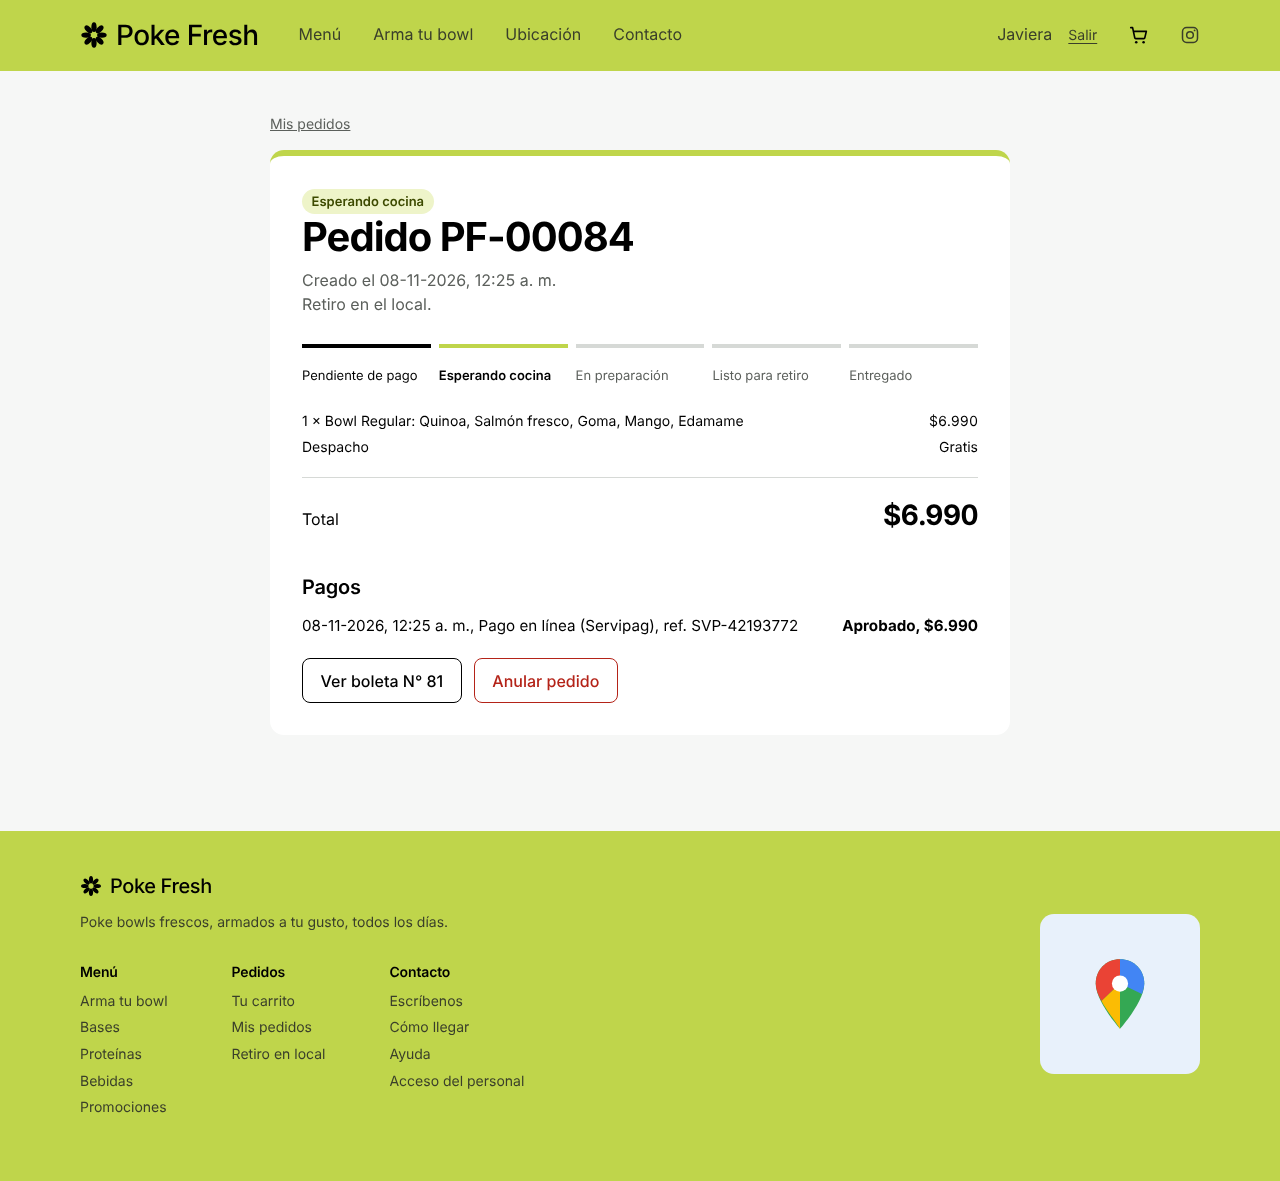
\includegraphics[width=\linewidth,height=0.85\textheight,keepaspectratio]{../evidencias/pantallas/06-pedido-pagado-graphql.png}
\caption{Pantalla del pedido (06-pedido-pagado-graphql.png): el pedido, servicio de pedidos, junto a la sección “Pagos”, servicio de pagos, obtenidos con resumenPedido}
\end{figure}

\begin{figure}[H]
\centering
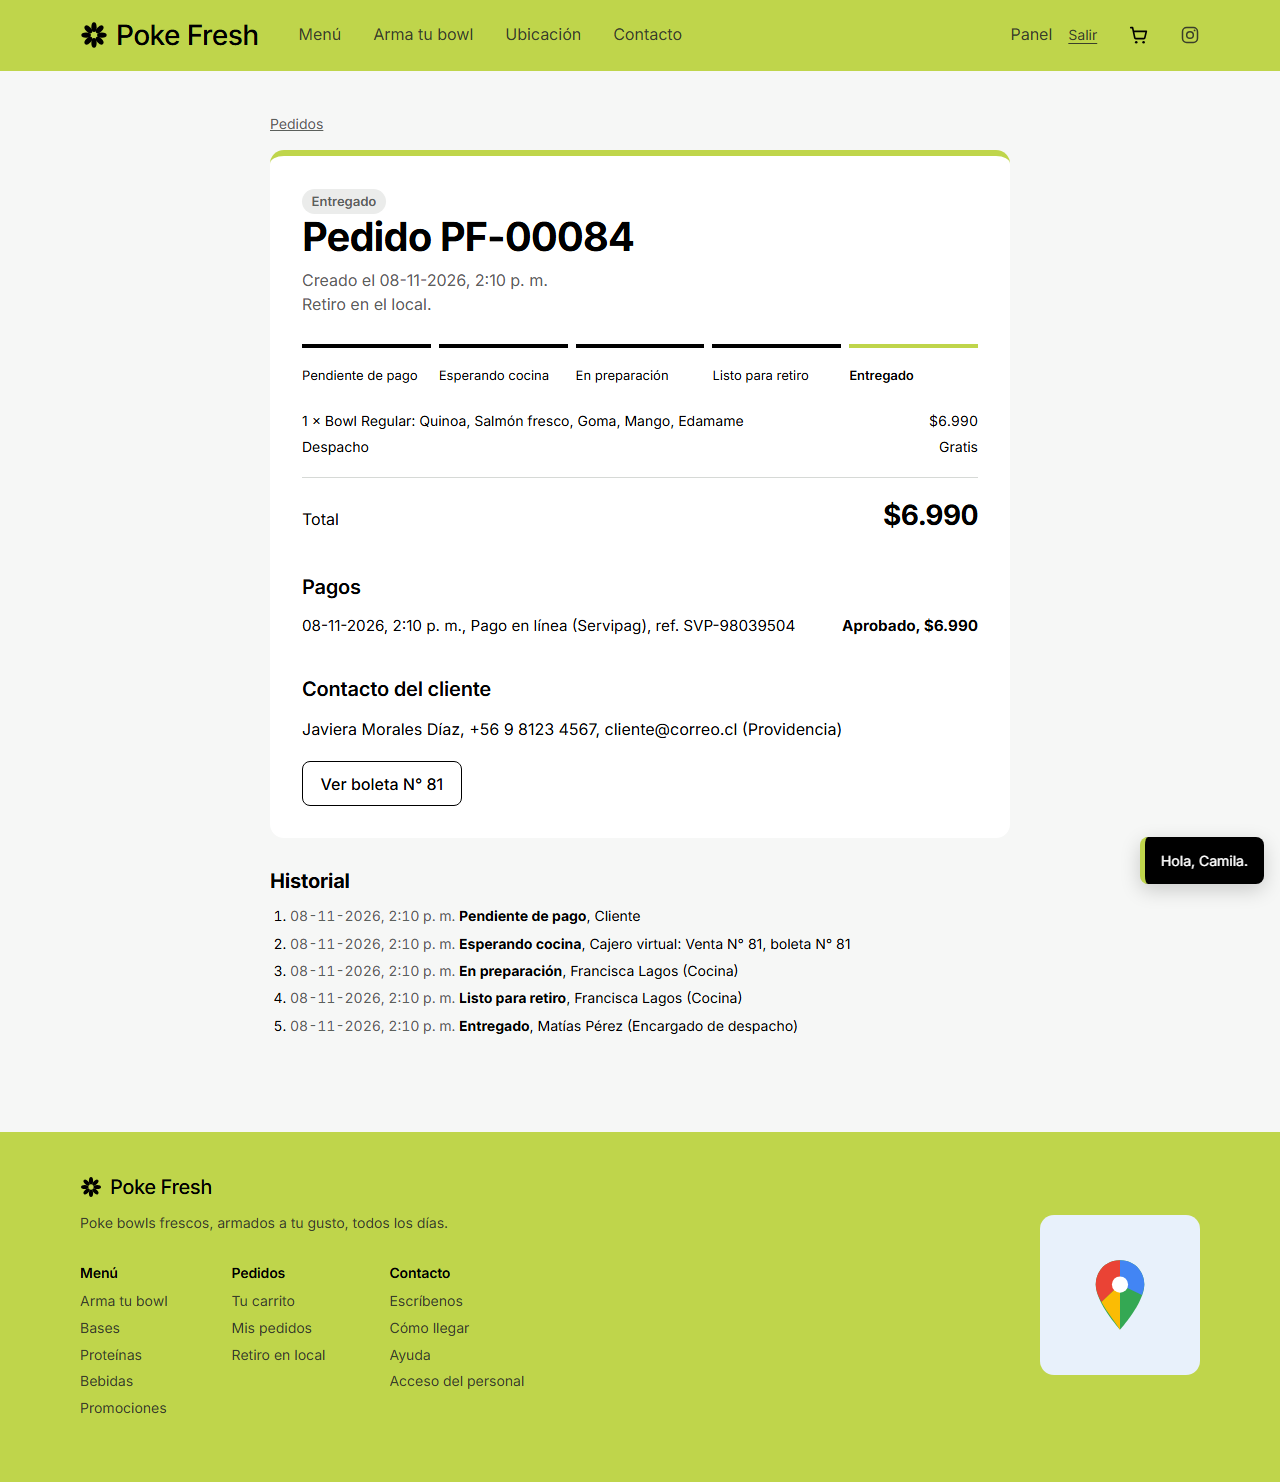
\includegraphics[width=\linewidth,height=0.85\textheight,keepaspectratio]{../evidencias/pantallas/14-pedido-vista-admin.png}
\caption{Vista del administrador (14-pedido-vista-admin.png): además aparece “Contacto del cliente”, servicio de clientes, solo para admin}
\end{figure}

\begin{figure}[H]
\centering
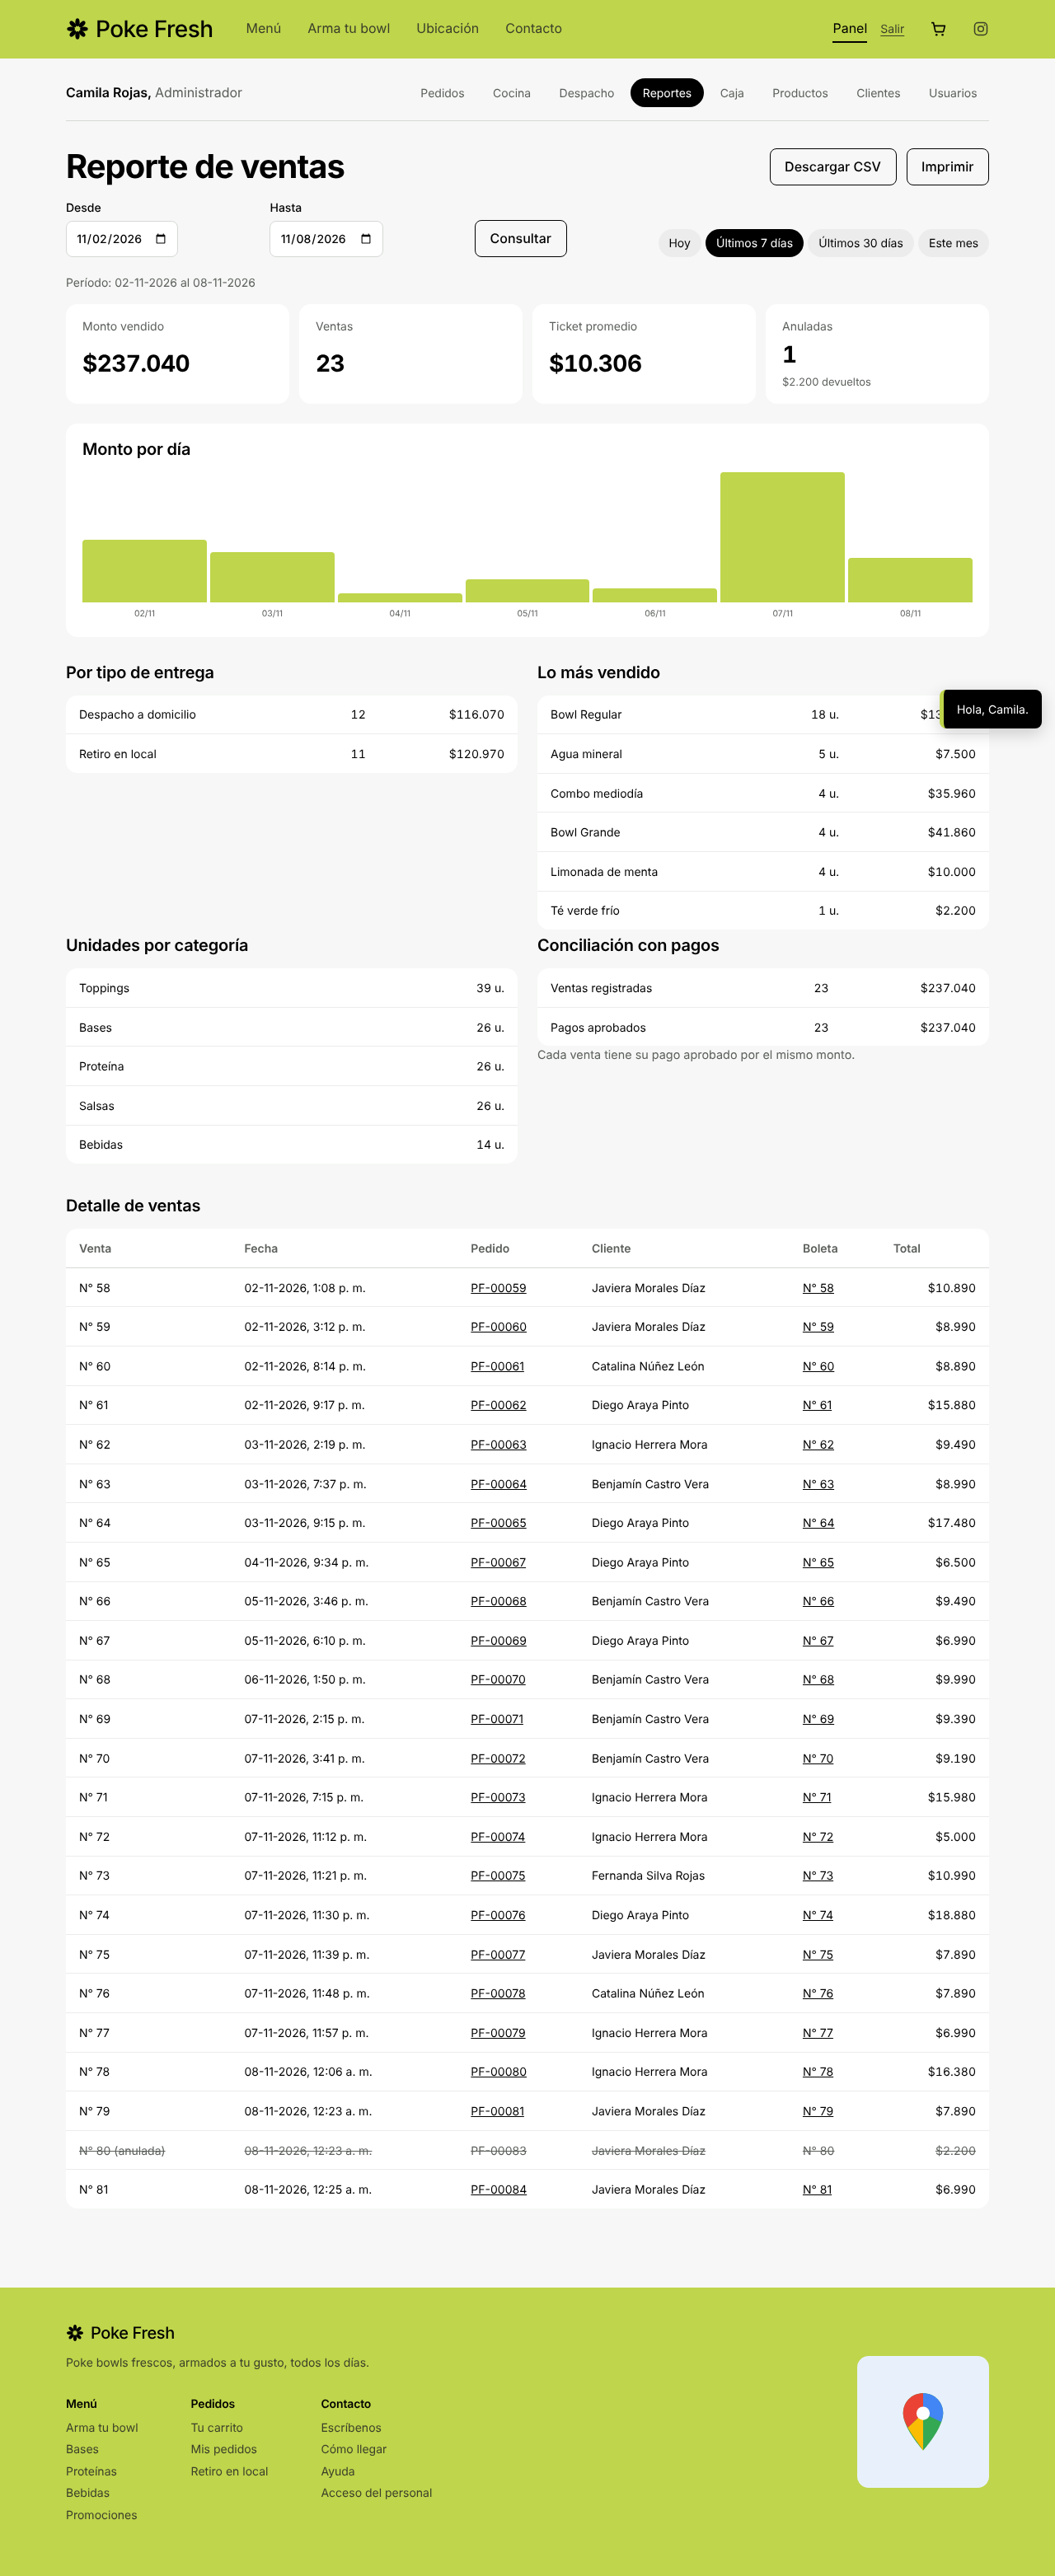
\includegraphics[width=\linewidth,height=0.85\textheight,keepaspectratio]{../evidencias/pantallas/11-reportes-graphql.png}
\caption{Reportes (11-reportes-graphql.png): “Unidades por categoría” y “Conciliación con pagos”, desde reporteVentas}
\end{figure}

\texttt{recorrido.\allowbreak{}json} lista las rutas de la API que usó el navegador: todas bajo \texttt{/\allowbreak{}api/\allowbreak{}v1}; ninguna a un servicio interno.


\textbf{Qué comprobamos.} Que la consulta junta de verdad datos de tres o cuatro servicios; que cada servicio mantiene su autoridad (la propiedad del pedido la decide pedidos); que pedir campos de más no filtra datos restringidos (si un cliente pide \texttt{cliente \{ email \}}, recibe PROHIBIDO); y que la red privada y los permisos funcionan con el sistema en marcha (casos 7.5, 7.9 y 8.1 a 8.3).


\clearpage
% Generado desde docs/INFORME.md. Editar libremente.

\section{9. Analítica y gRPC}

No toda necesidad de reporte exige un sistema de analítica aparte, ni todo mensaje entre servicios exige gRPC. Esta sección decide con números si hacían falta: primero qué carga tiene el negocio y qué se midió, luego por qué no se implementó cada componente y, por último, las razones a favor y en contra de gRPC.


La decisión, con contexto, alternativas y consecuencias, está en ADR 0001 (\texttt{docs/\allowbreak{}adr/\allowbreak{}0001-\allowbreak{}analitica-\allowbreak{}y-\allowbreak{}grpc.\allowbreak{}md}).


\subsection{Matriz de necesidades}

{\small
\setlength{\tabcolsep}{3pt}\renewcommand{\arraystretch}{1.15}
\begin{longtable}{|>{\raggedright\arraybackslash}p{\dimexpr 0.1919\linewidth-2\tabcolsep\relax}|>{\raggedright\arraybackslash}p{\dimexpr 0.3858\linewidth-2\tabcolsep\relax}|>{\raggedright\arraybackslash}p{\dimexpr 0.1805\linewidth-2\tabcolsep\relax}|>{\raggedright\arraybackslash}p{\dimexpr 0.2417\linewidth-2\tabcolsep\relax}|}
\hline
\textbf{Necesidad} & \textbf{Valor} & \textbf{Proyección / medición} & \textbf{¿Requiere analítica separada o gRPC?} \\ \hline
\endfirsthead
\hline
\textbf{Necesidad} & \textbf{Valor} & \textbf{Proyección / medición} & \textbf{¿Requiere analítica separada o gRPC?} \\ \hline
\endhead
Volumen de datos & \textasciitilde{}55.000 pedidos/año, < 100 MB & Proyección & No \\ \hline
Concurrencia en el pico & \textasciitilde{}5 peticiones/s & Proyección & No \\ \hline
Capacidad medida & 209 a 316 peticiones/s, p95 92 a 147 ms, 0 \% de error (en Docker, con TLS) & \textbf{Medición} (\texttt{evidencias/\allowbreak{}carga.\allowbreak{}md}) & No \\ \hline
Tamaño de mensaje & < 10 KB & Medición & No \\ \hline
Frecuencia del reporte & Pocas veces al día & Proyección & No: consulta indexada en pedidos \\ \hline
Latencia aceptada del reporte & $\leq$ 2 s & Objetivo & Cumple \\ \hline
Streaming & No se necesita (aviso a cocina en segundos) & Requisito & No; los avisos asíncronos van por ActiveMQ \\ \hline
\end{longtable}
}

\subsection{La prueba de carga}

La decisión de no separar un servicio de analítica ni usar gRPC se apoya en una \textbf{medición}, no en una proyección. El detalle y los comandos para repetirla están en \texttt{evidencias/\allowbreak{}carga.\allowbreak{}md}.


\begin{itemize}[nosep,leftmargin=*]
\item \textbf{Entorno:} un PC con Windows 11, AMD Ryzen 7 5800H (16 hilos), 16 GB de RAM y Docker Desktop (el motor ve 16 CPU y 15,3 GiB). El generador de carga, \texttt{pruebas/\allowbreak{}carga/\allowbreak{}carga.\allowbreak{}mjs}, corre en el mismo equipo, fuera de Docker, y entra por el puerto 8080 por HTTPS verificando el certificado; por eso compite por CPU con los contenedores y las latencias incluyen la red de Docker Desktop.
\item \textbf{Sistema:} el \texttt{docker-\allowbreak{}compose.\allowbreak{}yml} completo, con MongoDB, Vault y ActiveMQ reales, las dos redes y TLS en todos los saltos.
\item \textbf{Datos:} los de ejemplo (6 clientes, 80 pedidos, 29 productos) más lo que crean las pruebas de punta a punta.
\item \textbf{Carga:} 20 conexiones concurrentes durante 20 segundos por escenario, sin pausa entre peticiones: el peor caso, porque cada conexión pide apenas recibe la respuesta anterior.
\end{itemize}

{\scriptsize
\setlength{\tabcolsep}{3pt}\renewcommand{\arraystretch}{1.15}
\begin{longtable}{|>{\raggedright\arraybackslash}p{\dimexpr 0.1852\linewidth-2\tabcolsep\relax}|>{\raggedright\arraybackslash}p{\dimexpr 0.3000\linewidth-2\tabcolsep\relax}|>{\raggedleft\arraybackslash}p{\dimexpr 0.1190\linewidth-2\tabcolsep\relax}|>{\raggedleft\arraybackslash}p{\dimexpr 0.0903\linewidth-2\tabcolsep\relax}|>{\raggedleft\arraybackslash}p{\dimexpr 0.0650\linewidth-2\tabcolsep\relax}|>{\raggedleft\arraybackslash}p{\dimexpr 0.0734\linewidth-2\tabcolsep\relax}|>{\raggedleft\arraybackslash}p{\dimexpr 0.0734\linewidth-2\tabcolsep\relax}|>{\raggedleft\arraybackslash}p{\dimexpr 0.0937\linewidth-2\tabcolsep\relax}|}
\hline
\textbf{Escenario} & \textbf{Qué mide} & \textbf{Peticiones} & \textbf{Por segundo} & \textbf{p50} & \textbf{p95} & \textbf{p99} & \textbf{Errores} \\ \hline
\endfirsthead
\hline
\textbf{Escenario} & \textbf{Qué mide} & \textbf{Peticiones} & \textbf{Por segundo} & \textbf{p50} & \textbf{p95} & \textbf{p99} & \textbf{Errores} \\ \hline
\endhead
\texttt{GET /\allowbreak{}catalogo/\allowbreak{}items} (anónimo) & Lectura pública del catálogo en inventario, sin sesión & 6.339 & 316,4 & 61,4 ms & 91,6 ms & 116,3 ms & 0 \% \\ \hline
GraphQL \texttt{resumenPedido} (cliente) & Agregación de pedidos, pagos e inventario, con sesión & 4.195 & 209,1 & 89,1 ms & 146,8 ms & 202,5 ms & 0 \% \\ \hline
\texttt{GET /\allowbreak{}pedidos?\allowbreak{}cola=\allowbreak{}cocina} (cocina) & Cola de cocina: sesión, introspección y consulta a MongoDB & 5.113 & 254,8 & 77,6 ms & 110,0 ms & 146,7 ms & 0 \% \\ \hline
\end{longtable}
}

\textbf{CPU y memoria.} Se registraron con \texttt{docker stats}, en una sola muestra tomada durante el tercer escenario (100 \% equivale a un núcleo):


{\small
\setlength{\tabcolsep}{3pt}\renewcommand{\arraystretch}{1.15}
\begin{longtable}{|>{\raggedright\arraybackslash}p{\dimexpr 0.5799\linewidth-2\tabcolsep\relax}|>{\raggedleft\arraybackslash}p{\dimexpr 0.1747\linewidth-2\tabcolsep\relax}|>{\raggedleft\arraybackslash}p{\dimexpr 0.2454\linewidth-2\tabcolsep\relax}|}
\hline
\textbf{Contenedor} & \textbf{CPU} & \textbf{Memoria} \\ \hline
\endfirsthead
\hline
\textbf{Contenedor} & \textbf{CPU} & \textbf{Memoria} \\ \hline
\endhead
pedidos & 108 \% & 63 MiB \\ \hline
MongoDB & 91 \% & 359 MiB \\ \hline
API Gateway (TLS y reenvío) & 65 \% & 130 MiB \\ \hline
Auth Service (introspección en cada petición) & 40 \% & 73 MiB \\ \hline
inventario, clientes, pagos & 0,1 \% & de 49 a 61 MiB \\ \hline
GraphQL Gateway (sin uso en este escenario) & 0 \% & 151 MiB \\ \hline
\end{longtable}
}

Con una sola muestra no se pueden sacar conclusiones finas sobre cuánto consume cada pieza: sirve para ver el orden de magnitud y que ningún contenedor se acerca a un límite de memoria. Tampoco permite comparar con otra tecnología.


\textbf{Comparación con los objetivos} (ADR 0001):


{\small
\setlength{\tabcolsep}{3pt}\renewcommand{\arraystretch}{1.15}
\begin{longtable}{|>{\raggedright\arraybackslash}p{\dimexpr 0.4475\linewidth-2\tabcolsep\relax}|>{\raggedright\arraybackslash}p{\dimexpr 0.3299\linewidth-2\tabcolsep\relax}|>{\raggedright\arraybackslash}p{\dimexpr 0.2226\linewidth-2\tabcolsep\relax}|}
\hline
\textbf{Objetivo} & \textbf{Medido} & \textbf{¿Cumple?} \\ \hline
\endfirsthead
\hline
\textbf{Objetivo} & \textbf{Medido} & \textbf{¿Cumple?} \\ \hline
\endhead
p95 menor a 300 ms en catálogo y colas & 92 ms y 110 ms & Sí \\ \hline
p95 menor a 500 ms en agregaciones GraphQL & 147 ms & Sí \\ \hline
Soportar el pico estimado de 5 peticiones por segundo con 0 \% de error & De 209 a 316 peticiones por segundo, 0 \% de error & Sí, con un margen de 42 a 63 veces \\ \hline
\end{longtable}
}

\subsection{Por qué no se implementa cada componente}

{\small
\setlength{\tabcolsep}{3pt}\renewcommand{\arraystretch}{1.15}
\begin{longtable}{|>{\raggedright\arraybackslash}p{\dimexpr 0.2286\linewidth-2\tabcolsep\relax}|>{\raggedright\arraybackslash}p{\dimexpr 0.1322\linewidth-2\tabcolsep\relax}|>{\raggedright\arraybackslash}p{\dimexpr 0.3196\linewidth-2\tabcolsep\relax}|>{\raggedright\arraybackslash}p{\dimexpr 0.3196\linewidth-2\tabcolsep\relax}|}
\hline
\textbf{Componente} & \textbf{¿Se implementa?} & \textbf{Requisito del caso y carga que lo justificarían} & \textbf{Por qué no} \\ \hline
\endfirsthead
\hline
\textbf{Componente} & \textbf{¿Se implementa?} & \textbf{Requisito del caso y carga que lo justificarían} & \textbf{Por qué no} \\ \hline
\endhead
Servicio de analítica separado & No & Reportes de ventas por período, unas pocas veces al día & Los resuelve una consulta indexada en pedidos (< 100 MB al año) más la agregación GraphQL (S32); un almacén aparte sería costo sin beneficio \\ \hline
gRPC unary (cotizar, reservar) & No & 2 a 4 llamadas internas por petición, mensajes de menos de 10 KB & REST con JSON cumple la latencia con margen de 42 a 63 veces el pico \\ \hline
gRPC streaming (avisos a cocina) & No & Cocina se entera en segundos, no en milisegundos & La pantalla consulta cada 8 s; el evento ya sale por ActiveMQ, que además recupera lo pendiente tras una desconexión \\ \hline
Trabajo largo asíncrono con identificador & No & No hay operaciones largas & El correo y la boleta ya son asíncronos por ActiveMQ y no bloquean el pago \\ \hline
Carga y fallos & Sí, medidos & Objetivos de p95 y 0 \% de error (ADR 0001) & \texttt{evidencias/\allowbreak{}carga.\allowbreak{}md} (tres escenarios) y pruebas de servicio caído (\texttt{502}), Vault caído (\texttt{503}) y error parcial en GraphQL \\ \hline
\end{longtable}
}

\subsection{gRPC: por qué sí y por qué no}

\textbf{Por qué sí podría usarse.} Aporta contratos tipados y generados (\texttt{.\allowbreak{}proto}), plazos y cancelación entre servicios, streaming del servidor con control de flujo, HTTP/2 con mensajes binarios y TLS o TLS mutuo con identidad en metadatos.


\textbf{Por qué no se usa en este caso.}


\begin{itemize}[nosep,leftmargin=*]
\item \textbf{Ningún flujo lo necesita.} Todas las llamadas internas son puntuales y pequeñas (menos de 10 KB; de 2 a 4 por petición): cotizar y reservar (una por pedido), ficha del cliente, confirmar un pago y las lecturas del GraphQL con DataLoader. Ninguna es de alta frecuencia ni larga.
\item \textbf{No hay un requisito de streaming.} Cocina debe enterarse en segundos; el evento sale por ActiveMQ y la pantalla consulta cada 8 s.
\item \textbf{Lo que daría ya está cubierto:} plazo de 4 s por llamada interna (\texttt{502/\allowbreak{}504}), \texttt{X-\allowbreak{}Request-\allowbreak{}Id} e identidad propagados, operaciones idempotentes, TLS entre todos los saltos y contratos validados en el servidor con pruebas.
\item \textbf{El navegador no habla gRPC.} Habría que mantener REST hacia afuera y \texttt{.\allowbreak{}proto} hacia adentro para lo mismo, o agregar un proxy gRPC-Web.
\item \textbf{Costo de operación:} generación de código en Node y Python, un servidor gRPC junto a cada FastAPI y rehacer \texttt{healthcheck}, pruebas y controles de seguridad para otro protocolo.
\item \textbf{El rendimiento ya cumple:} 209 a 316 peticiones/s con REST y TLS, de 42 a 63 veces el pico proyectado.
\end{itemize}

\textbf{Limitación.} No se midió gRPC contra REST; por eso no se afirma que sea más rápido, más lento ni que consuma más o menos CPU o memoria. La decisión se apoya en que el caso no tiene un requisito que lo justifique y en la capacidad medida del diseño actual.


\textbf{Cuándo sería sí.} Un consumidor privado que necesite un flujo continuo de eventos con reanudación (por ejemplo, un monitor de despacho en tiempo real), una llamada interna que supere la capacidad medida, varios equipos o lenguajes que exijan contratos generados, o una operación larga que haya que cancelar. En ese caso: \texttt{unary} con plazo de 4 s para cotizar y reservar, un stream del servidor para eventos de pedido con el último evento recibido para reanudar sin duplicar, identidad en metadatos y un adaptador con Server-Sent Events en el gateway para el navegador. Es una propuesta y \textbf{no está implementada ni probada}.


El análisis completo, con una evaluación flujo por flujo, está en el ADR 0001 (\texttt{docs/\allowbreak{}adr/\allowbreak{}0001-\allowbreak{}analitica-\allowbreak{}y-\allowbreak{}grpc.\allowbreak{}md}).


\textbf{Conclusión:} no se implementa un servicio de analítica separado ni gRPC, porque la carga proyectada es entre 42 y 63 veces menor que la medida y no hay flujos de streaming. La alternativa implementada (reporte en pedidos + agregación GraphQL + eventos por ActiveMQ) cumple los objetivos con la prueba de carga como evidencia. El ADR indica cuándo revisar la decisión.


\clearpage
% Generado desde docs/INFORME.md. Editar libremente.

\section{10. Backend completo e integración verificable}

\subsection{Qué se entrega}

{\small
\setlength{\tabcolsep}{3pt}\renewcommand{\arraystretch}{1.15}
\begin{longtable}{|>{\raggedright\arraybackslash}p{\dimexpr 0.3248\linewidth-2\tabcolsep\relax}|>{\raggedright\arraybackslash}p{\dimexpr 0.6752\linewidth-2\tabcolsep\relax}|}
\hline
\textbf{Pieza} & \textbf{Dónde} \\ \hline
\endfirsthead
\hline
\textbf{Pieza} & \textbf{Dónde} \\ \hline
\endhead
Código del frontend & \texttt{frontend/\allowbreak{}} \\ \hline
Código del backend & \texttt{gateway/\allowbreak{}}, \texttt{auth-\allowbreak{}service/\allowbreak{}}, \texttt{graphql-\allowbreak{}gateway/\allowbreak{}}, \texttt{servicios/\allowbreak{}} \\ \hline
Despliegue reproducible & \texttt{docker-\allowbreak{}compose.\allowbreak{}yml}, \texttt{Dockerfile} de cada componente, \texttt{vault/\allowbreak{}} \\ \hline
Persistencia y creación & MongoDB con una base y un usuario por servicio; índices creados al arrancar (\texttt{preparar} en cada servicio); datos ficticios con \texttt{servicios/\allowbreak{}scripts/\allowbreak{}semilla.\allowbreak{}py} \\ \hline
Contratos REST & Sección 1 y OpenAPI de cada servicio \\ \hline
Contrato GraphQL & Sección 8 y \texttt{graphql-\allowbreak{}gateway/\allowbreak{}src/\allowbreak{}graphql/\allowbreak{}esquema.\allowbreak{}js} \\ \hline
Contratos gRPC & No aplica (ADR 0001) \\ \hline
Pruebas automatizadas & 86 unitarias y de integración + 23 de punta a punta (contra Docker, con TLS) + recorrido de pantallas + carga \\ \hline
Instrucciones & \texttt{README.\allowbreak{}md} \\ \hline
\end{longtable}
}

\subsection{Pruebas y resultados}

{\small
\setlength{\tabcolsep}{3pt}\renewcommand{\arraystretch}{1.15}
\begin{longtable}{|>{\raggedright\arraybackslash}p{\dimexpr 0.2074\linewidth-2\tabcolsep\relax}|>{\raggedleft\arraybackslash}p{\dimexpr 0.2069\linewidth-2\tabcolsep\relax}|>{\raggedright\arraybackslash}p{\dimexpr 0.4017\linewidth-2\tabcolsep\relax}|>{\raggedright\arraybackslash}p{\dimexpr 0.1840\linewidth-2\tabcolsep\relax}|}
\hline
\textbf{Conjunto} & \textbf{Cantidad} & \textbf{Qué cubre} & \textbf{Resultado} \\ \hline
\endfirsthead
\hline
\textbf{Conjunto} & \textbf{Cantidad} & \textbf{Qué cubre} & \textbf{Resultado} \\ \hline
\endhead
\texttt{servicios/\allowbreak{}tests} (pytest) & 37 & Reglas de cada servicio, propiedad, cotización, stock, idempotencia, firma, Vault caído (503), servicio caído (502), datos de ejemplo, URI de Mongo con TLS & 37/37 \\ \hline
\texttt{auth-\allowbreak{}service/\allowbreak{}test} & 20 & Login, bloqueo, expiración, revocación, verificación, permisos por cliente, hash y pepper, Vault sellado & 20/20 \\ \hline
\texttt{gateway/\allowbreak{}test} & 18 & Matriz de rutas, roles, cabeceras falsificadas, cookie, CSRF, webhook, Vault y servicio caídos, límite, healthcheck, HSTS & 18/18 \\ \hline
\texttt{graphql-\allowbreak{}gateway/\allowbreak{}test} & 11 & Agregación, batching, identidad, autorización por campo, error parcial, límites, paginación & 11/11 \\ \hline
\texttt{pruebas/\allowbreak{}e2e/\allowbreak{}casos.\allowbreak{}py -\allowbreak{}-\allowbreak{}docker} & 23 & Casos del módulo 7 y del 10 contra el sistema levantado en Docker, por HTTPS; los casos 7.9, 7.10 y 10.7 se ejecutan dentro de la red privada & 23/23 \\ \hline
\texttt{pruebas/\allowbreak{}e2e/\allowbreak{}pantallas.\allowbreak{}py} & 16 pantallas de escritorio + 6 móviles & Flujos principales en el navegador, en escritorio (1280×900) y en móvil (375×812, táctil) & Completo, sin errores de consola \\ \hline
\texttt{pruebas/\allowbreak{}carga/\allowbreak{}carga.\allowbreak{}mjs} & 3 escenarios & Rendimiento contra el sistema en Docker & 0 \% de error \\ \hline
\end{longtable}
}

\subsection{Evidencia en móvil}

El recorrido repite seis pantallas en un teléfono emulado (375×812, táctil), contra el mismo sistema en Docker y las mismas APIs: inicio, menú, checkout, seguimiento del pedido, mis pedidos y despacho (\texttt{pantallas/\allowbreak{}m01-\allowbreak{}inicio-\allowbreak{}movil.\allowbreak{}png} a \texttt{m06-\allowbreak{}despacho-\allowbreak{}movil.\allowbreak{}png}). Para cada una el script comprueba que no hay scroll horizontal (\texttt{desbordeHorizontalMovil} en \texttt{pantallas/\allowbreak{}recorrido.\allowbreak{}json}: las seis en \texttt{false}). Los flujos de cocina y administración se verificaron solo en escritorio; el resto de los flujos se comparten entre ambos tamaños, porque es la misma SPA con diseño responsivo.


Además, \texttt{pruebas/\allowbreak{}e2e/\allowbreak{}movil.\allowbreak{}py} recorre en móvil (390×812, táctil, escala 2) una compra completa por HTTPS: inicio, menú, ingreso, checkout, pago, pasarela, pedido pagado con boleta e historial (\texttt{evidencias/\allowbreak{}movil/\allowbreak{}01-\allowbreak{}inicio.\allowbreak{}png} a \texttt{08-\allowbreak{}mis-\allowbreak{}pedidos.\allowbreak{}png}). Comprueba que todas las pantallas se sirven por HTTPS y que ninguna tiene scroll horizontal (\texttt{evidencias/\allowbreak{}movil/\allowbreak{}recorrido.\allowbreak{}json}), con 0 errores de consola. Es emulación de teléfono en Chromium, no un dispositivo real.


\subsection{Evidencia en navegador real}

\texttt{evidencias/\allowbreak{}navegador-\allowbreak{}real/\allowbreak{}} tiene 8 capturas de una compra completa hecha en Microsoft Edge por HTTPS (pedido PF-00086, pago aprobado en la pasarela de \texttt{https:\allowbreak{}/\allowbreak{}/\allowbreak{}localhost:\allowbreak{}9000}, boleta N° 83) y \texttt{datos-\allowbreak{}navegador.\allowbreak{}json} con el navegador, el protocolo, las URLs visitadas y la cabecera HSTS. Las capturas muestran la página y no la barra de direcciones; el protocolo consta en ese archivo. Antes de capturar se aceptó a mano la advertencia que el antivirus muestra por el certificado de prueba.


\subsection{Capturas de la ejecución}

Todas salen del sistema levantado en Docker, por HTTPS, con datos ficticios. Las de escritorio y las del teléfono emulado las generan \texttt{pruebas/\allowbreak{}e2e/\allowbreak{}pantallas.\allowbreak{}py} y \texttt{pruebas/\allowbreak{}e2e/\allowbreak{}movil.\allowbreak{}py}; las del navegador real se tomaron a mano en Edge. Las tres capturas de la sección 8 (pedido con pagos, vista del administrador y reportes) no se repiten aquí.


\subsubsection{Escritorio (Chromium, 1280×900): compra, cocina, despacho y administración}

\begin{figure}[H]\centering
\begin{minipage}[t]{0.485\linewidth}\centering
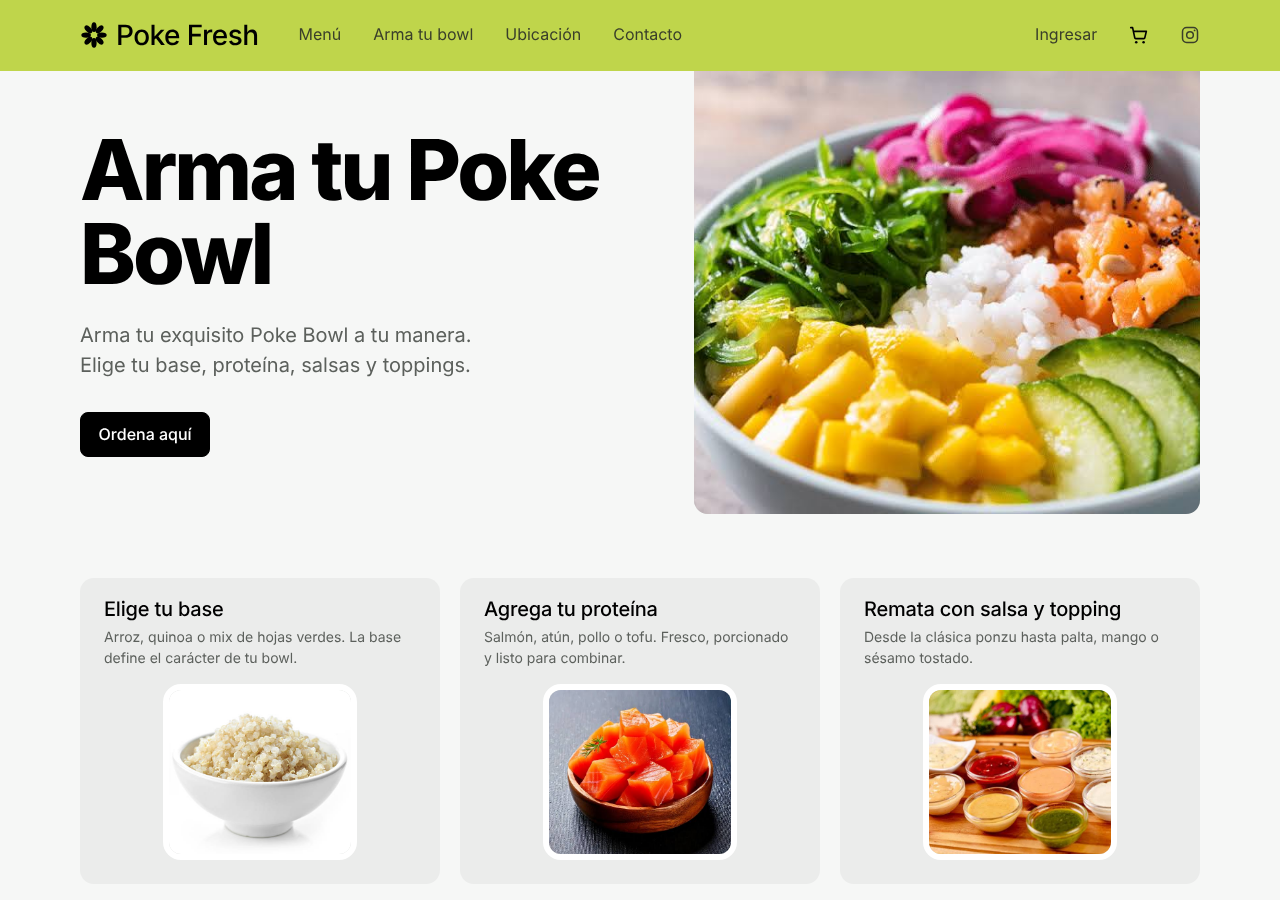
\includegraphics[width=\linewidth,height=0.42\textheight,keepaspectratio]{../evidencias/pantallas/01-inicio.png}
\captionof{figure}{Inicio: la tienda pública}
\end{minipage}\hfill
\begin{minipage}[t]{0.485\linewidth}\centering
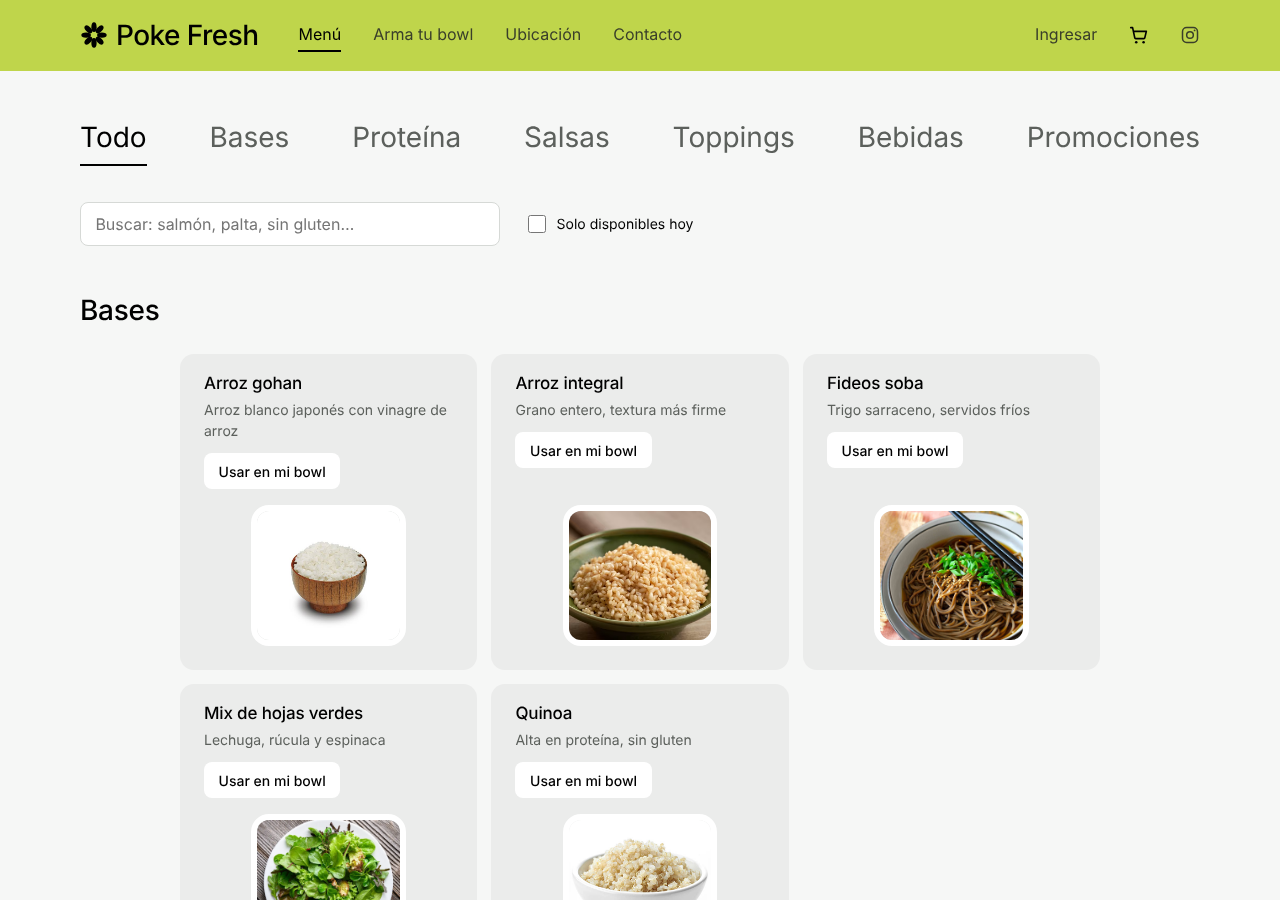
\includegraphics[width=\linewidth,height=0.42\textheight,keepaspectratio]{../evidencias/pantallas/02-menu-desde-inventario.png}
\captionof{figure}{Menú cargado desde el servicio de inventario}
\end{minipage}
\end{figure}

\begin{figure}[H]\centering
\begin{minipage}[t]{0.485\linewidth}\centering
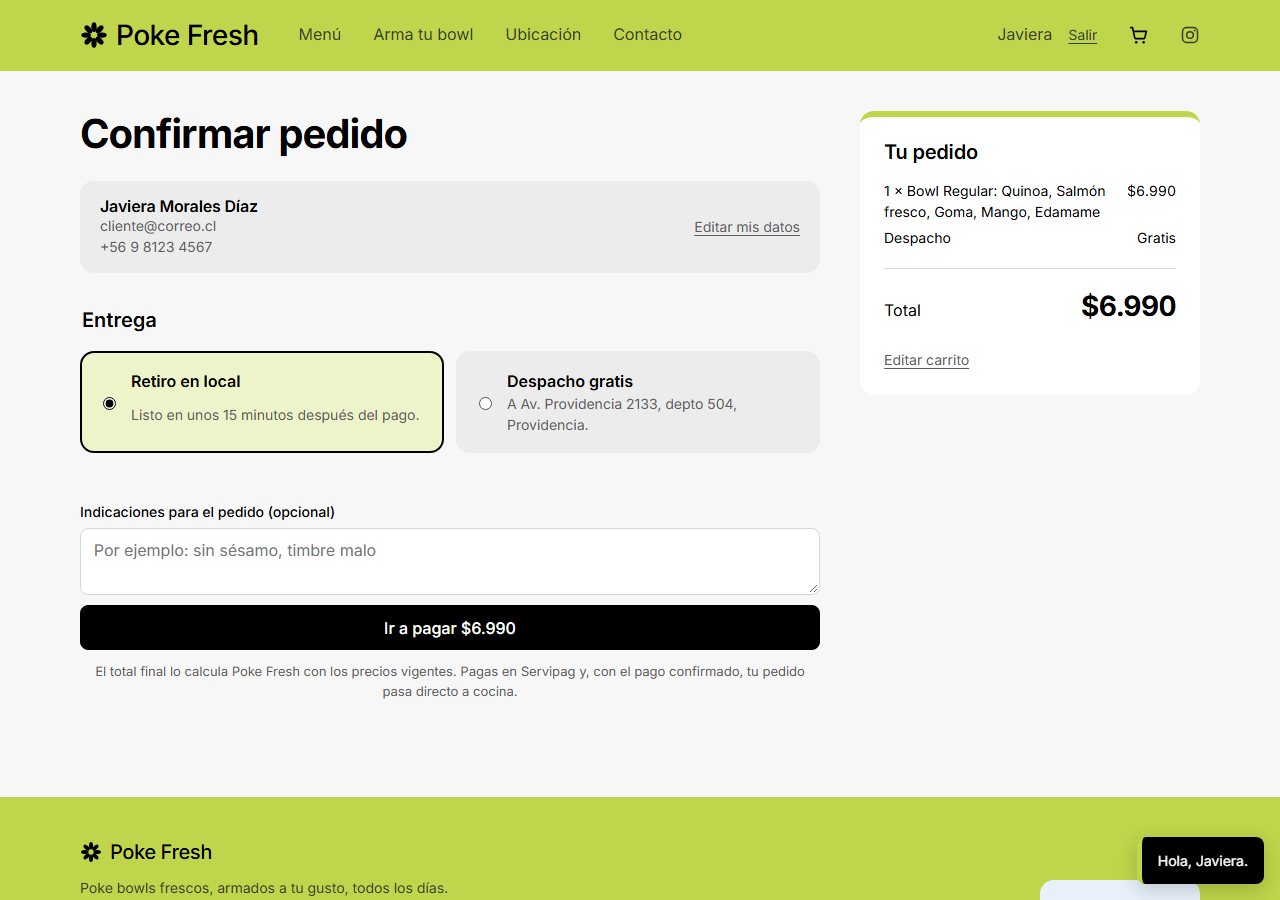
\includegraphics[width=\linewidth,height=0.42\textheight,keepaspectratio]{../evidencias/pantallas/03-checkout.png}
\captionof{figure}{Confirmar pedido: solo se manda la selección}
\end{minipage}\hfill
\begin{minipage}[t]{0.485\linewidth}\centering
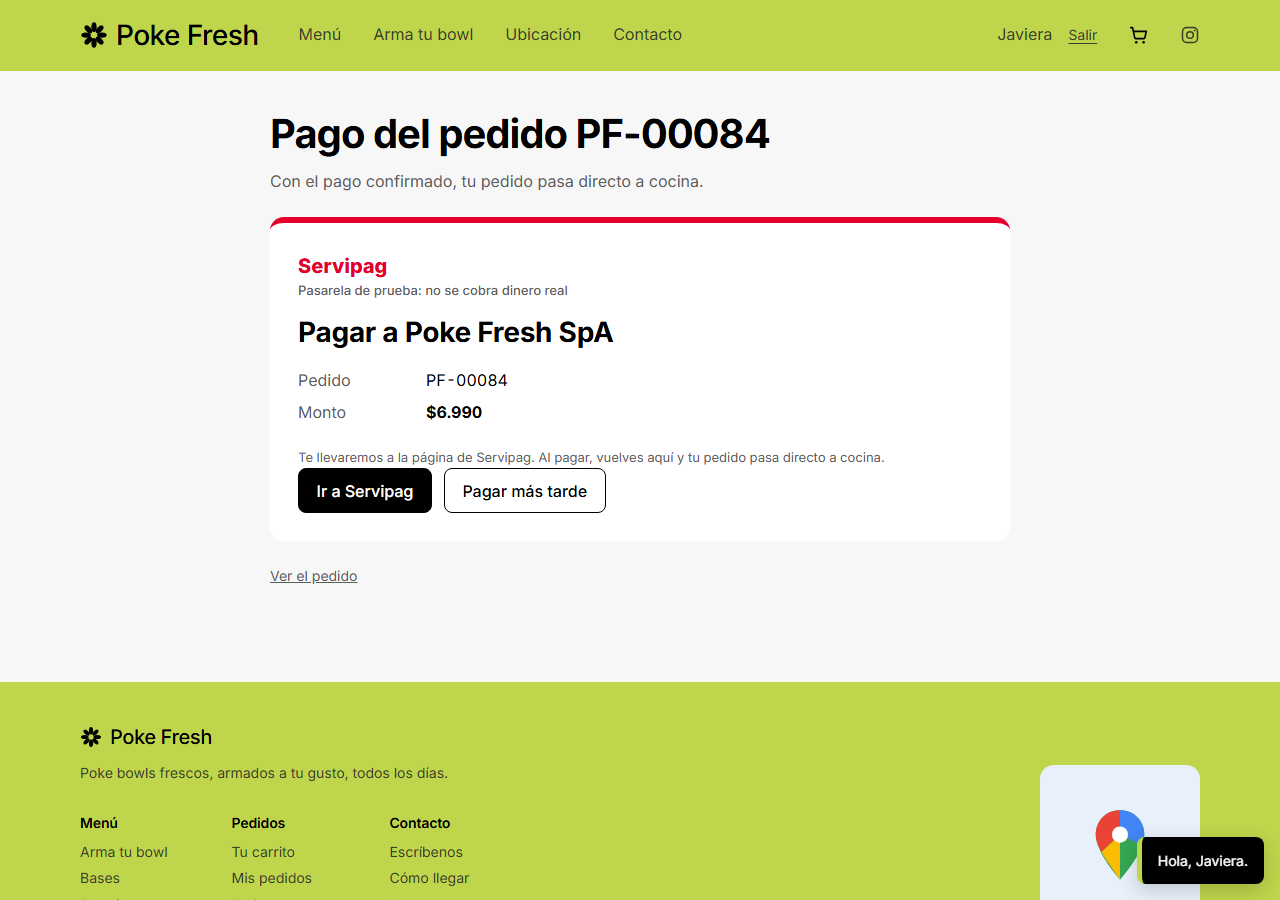
\includegraphics[width=\linewidth,height=0.42\textheight,keepaspectratio]{../evidencias/pantallas/04-pago.png}
\captionof{figure}{Pago: el pedido queda pendiente hasta que la pasarela confirme}
\end{minipage}
\end{figure}

\begin{figure}[H]
\centering
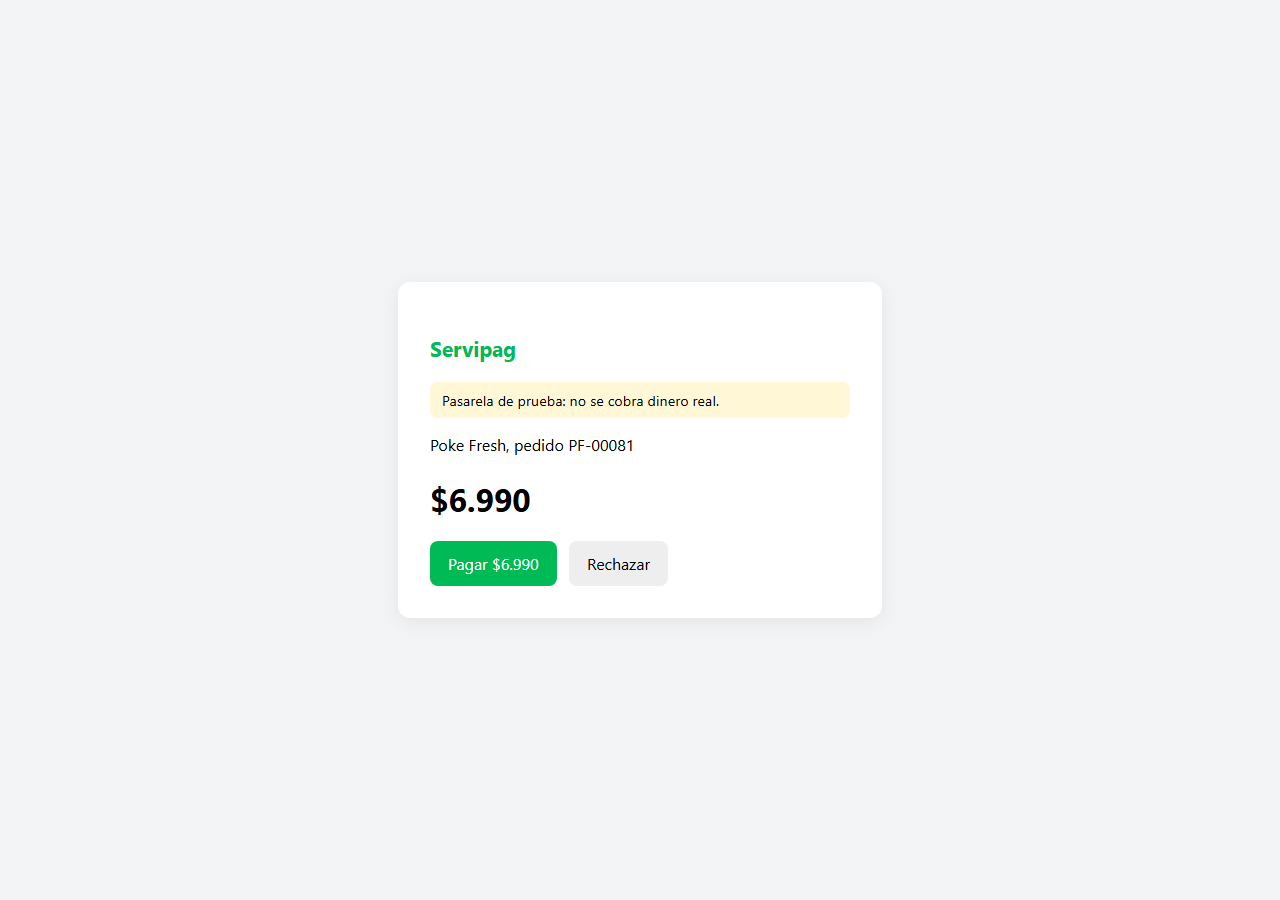
\includegraphics[width=\linewidth,height=0.85\textheight,keepaspectratio]{../evidencias/pantallas/05-pasarela-servipag.png}
\caption{Pasarela de pago simulada (Servipag), en el puerto 9000}
\end{figure}

\begin{figure}[H]\centering
\begin{minipage}[t]{0.485\linewidth}\centering
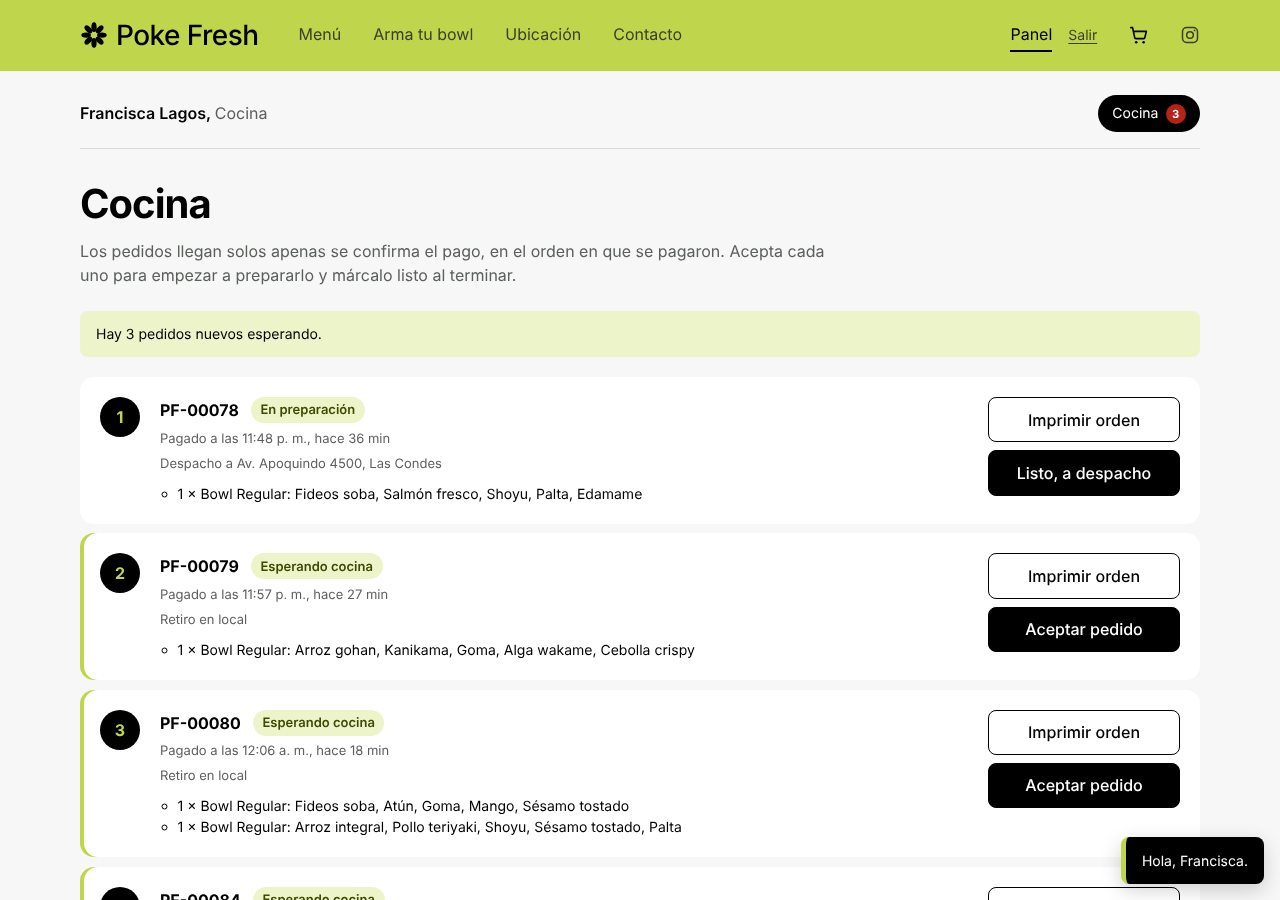
\includegraphics[width=\linewidth,height=0.42\textheight,keepaspectratio]{../evidencias/pantallas/07-cocina.png}
\captionof{figure}{Cocina: cola de pedidos pagados, en orden de llegada}
\end{minipage}\hfill
\begin{minipage}[t]{0.485\linewidth}\centering
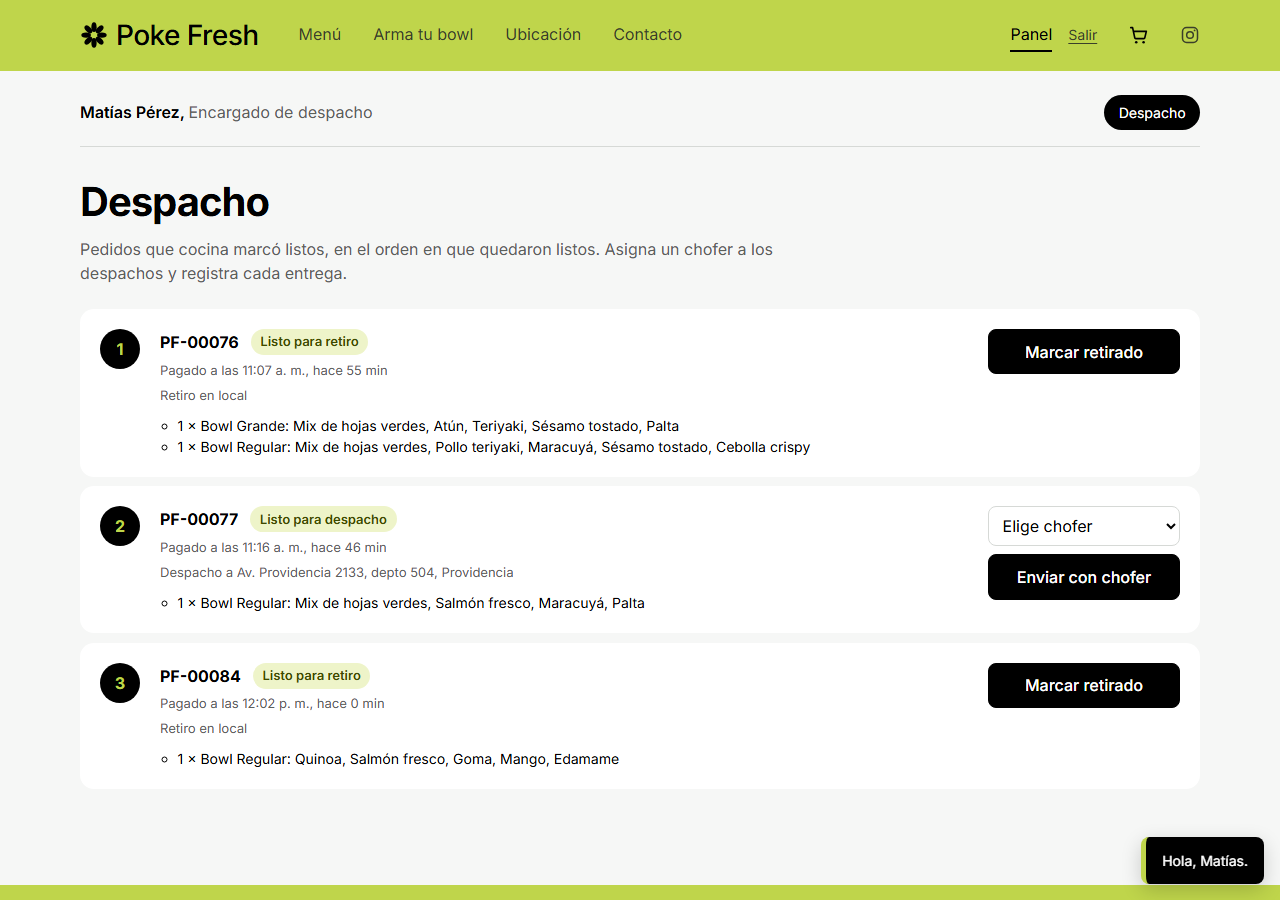
\includegraphics[width=\linewidth,height=0.42\textheight,keepaspectratio]{../evidencias/pantallas/08-despacho.png}
\captionof{figure}{Despacho: pedidos listos para entregar}
\end{minipage}
\end{figure}

\begin{figure}[H]
\centering
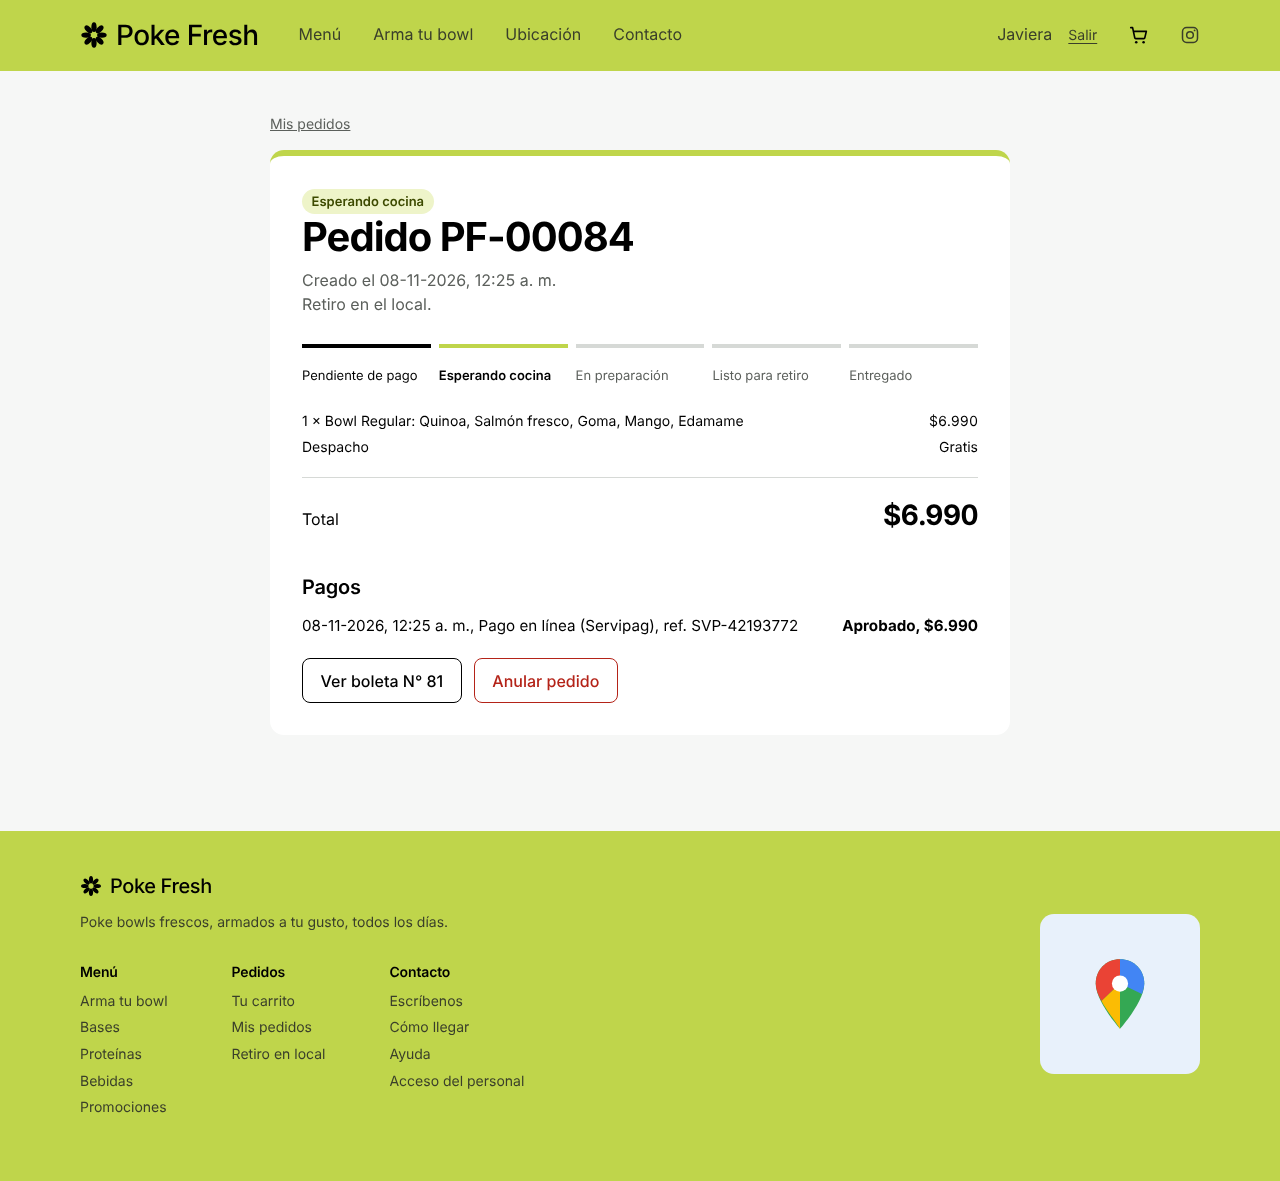
\includegraphics[width=\linewidth,height=0.85\textheight,keepaspectratio]{../evidencias/pantallas/09-seguimiento-entregado.png}
\caption{Seguimiento: el pedido en estado Entregado, con su boleta}
\end{figure}

\begin{figure}[H]
\centering
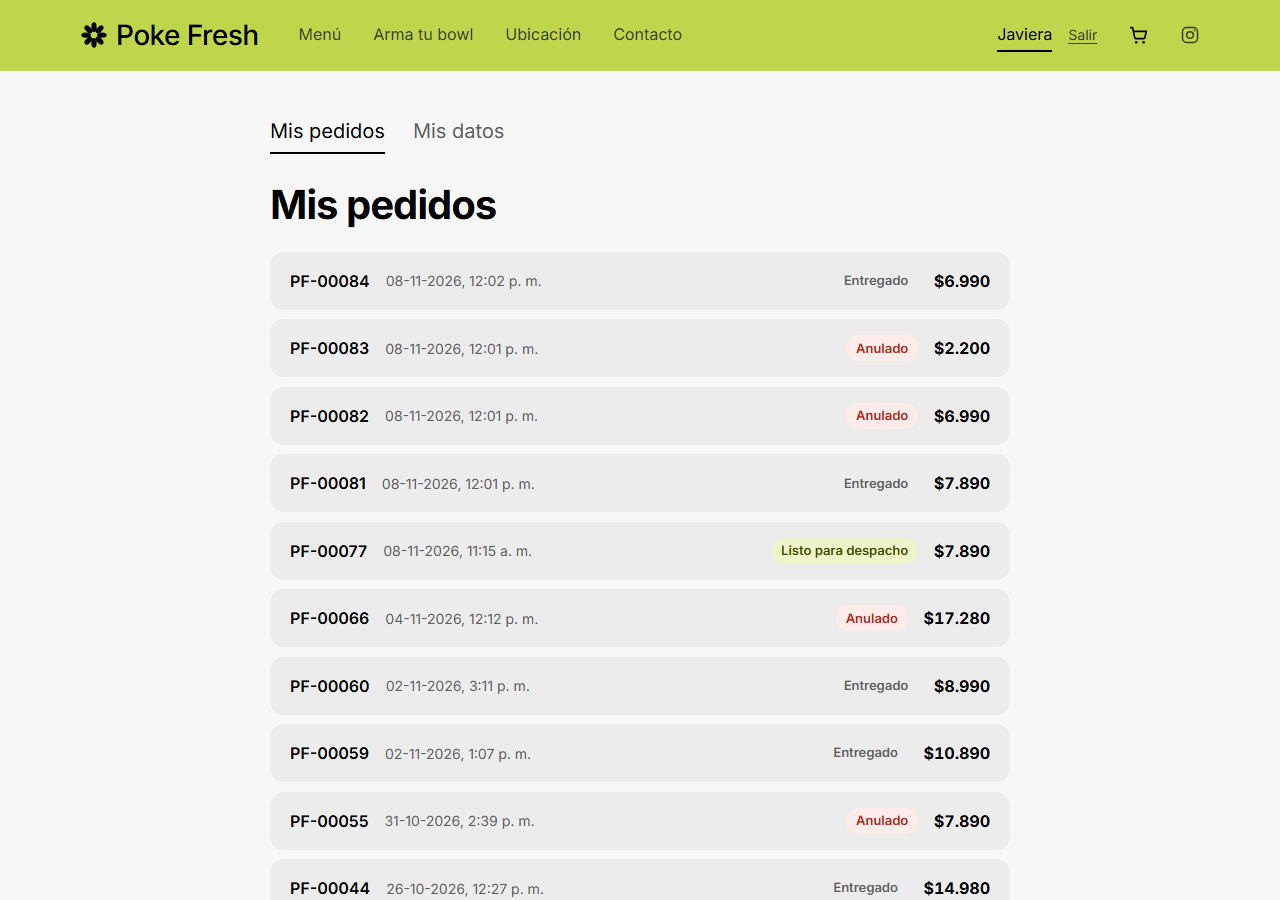
\includegraphics[width=\linewidth,height=0.85\textheight,keepaspectratio]{../evidencias/pantallas/10-mis-pedidos.png}
\caption{Mis pedidos: historial del cliente}
\end{figure}

\begin{figure}[H]\centering
\begin{minipage}[t]{0.485\linewidth}\centering
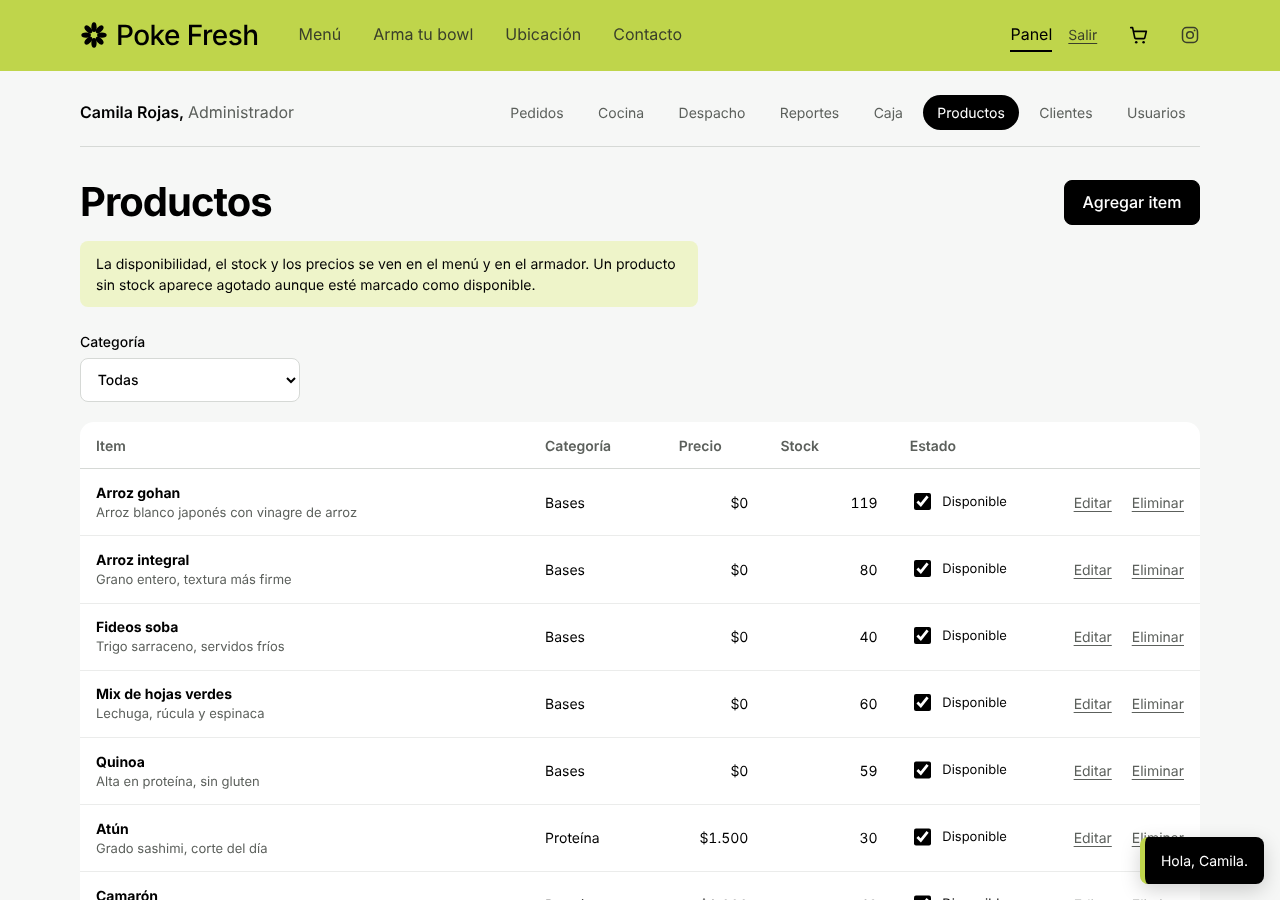
\includegraphics[width=\linewidth,height=0.42\textheight,keepaspectratio]{../evidencias/pantallas/12-productos-stock.png}
\captionof{figure}{Administración: productos y stock}
\end{minipage}\hfill
\begin{minipage}[t]{0.485\linewidth}\centering
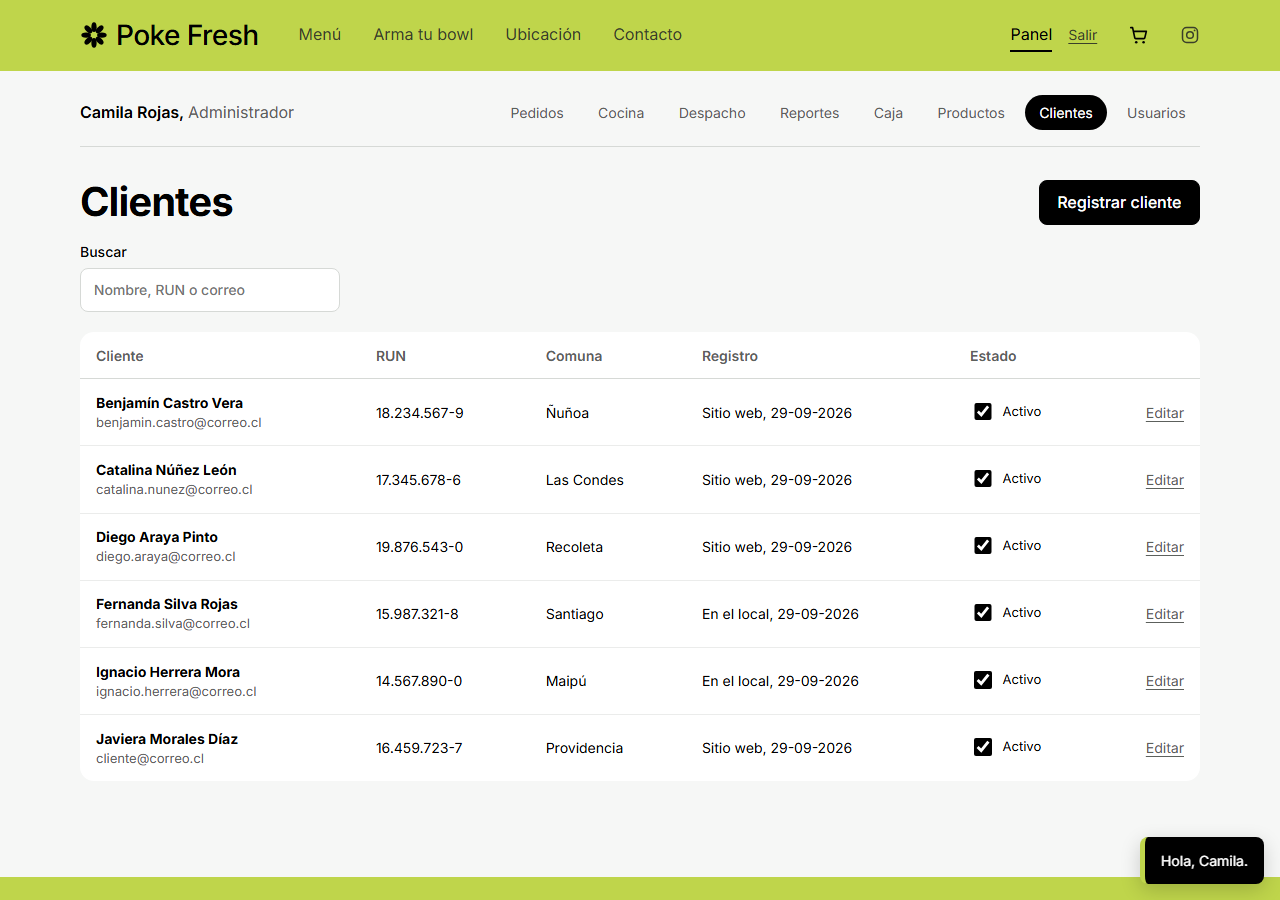
\includegraphics[width=\linewidth,height=0.42\textheight,keepaspectratio]{../evidencias/pantallas/13-clientes.png}
\captionof{figure}{Administración: clientes}
\end{minipage}
\end{figure}

\begin{figure}[H]\centering
\begin{minipage}[t]{0.485\linewidth}\centering
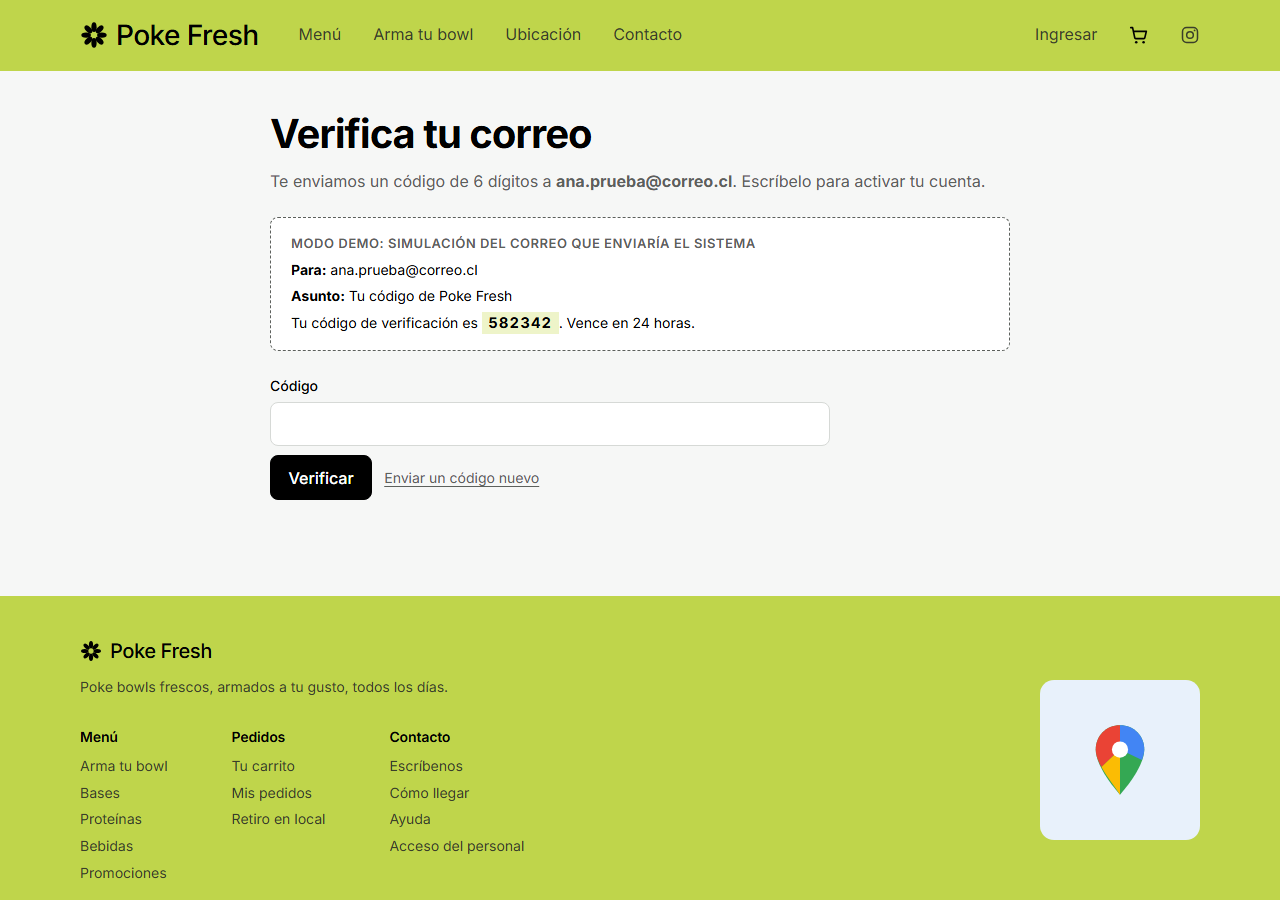
\includegraphics[width=\linewidth,height=0.42\textheight,keepaspectratio]{../evidencias/pantallas/15-verificacion-correo.png}
\captionof{figure}{Registro: verificación de correo (modo demo)}
\end{minipage}\hfill
\begin{minipage}[t]{0.485\linewidth}\centering
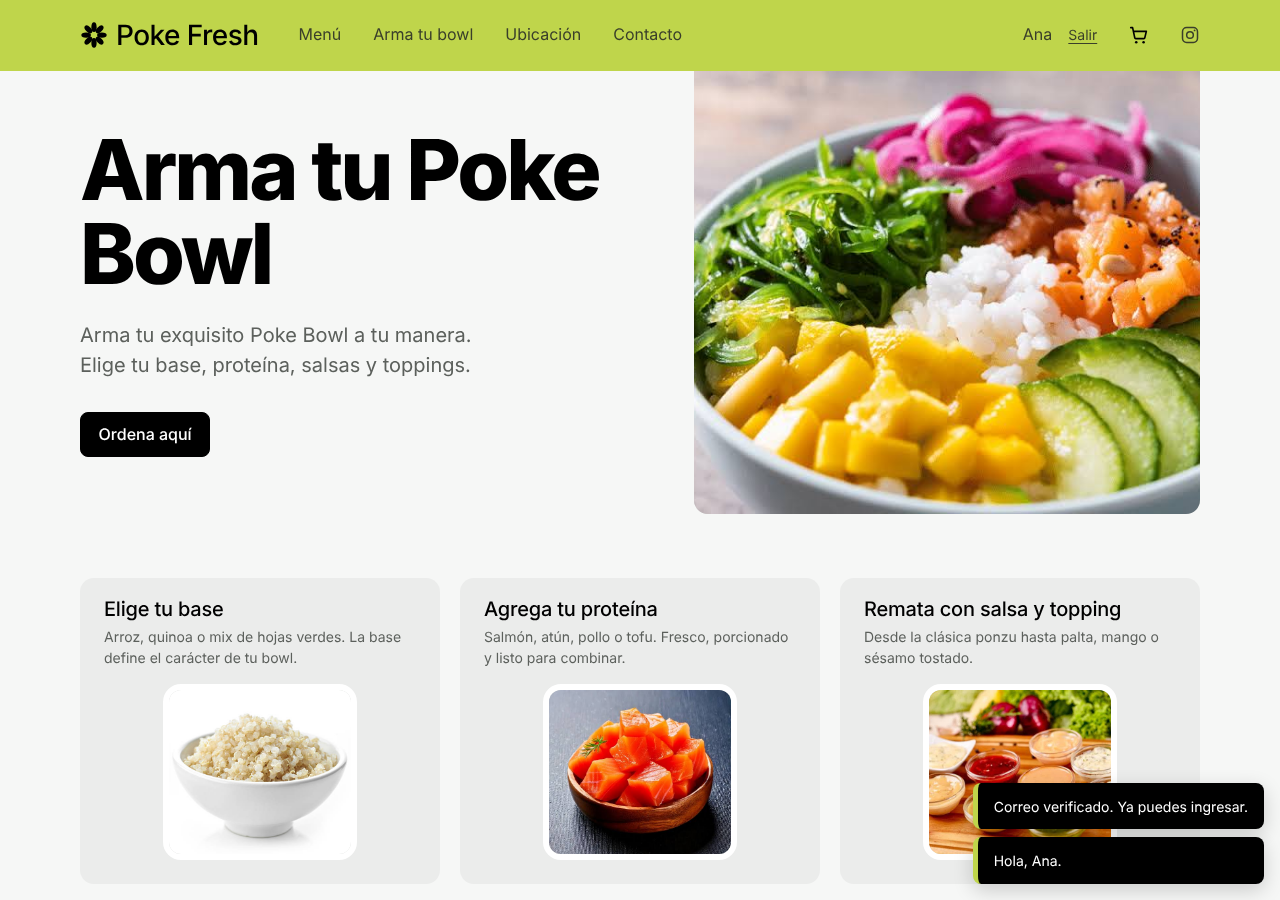
\includegraphics[width=\linewidth,height=0.42\textheight,keepaspectratio]{../evidencias/pantallas/16-cliente-nuevo-con-sesion.png}
\captionof{figure}{Cliente nuevo con sesión iniciada}
\end{minipage}
\end{figure}

\subsubsection{Teléfono emulado (Chromium, 390×812, táctil): compra completa}

\begin{figure}[H]\centering
\begin{minipage}[t]{0.242\linewidth}\centering
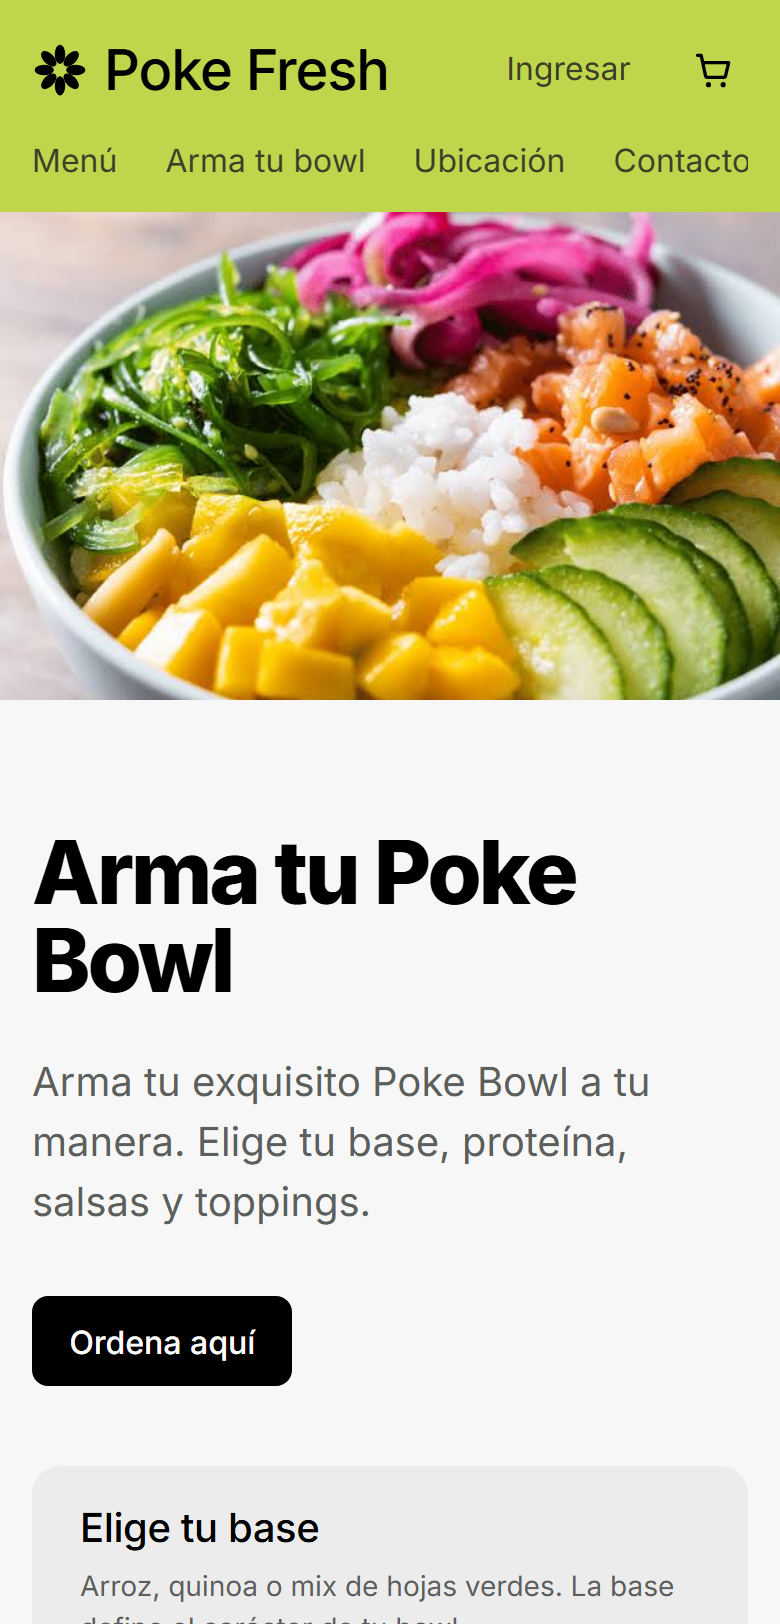
\includegraphics[width=\linewidth,height=0.4\textheight,keepaspectratio]{../evidencias/movil/01-inicio.png}
\captionof{figure}{Inicio}
\end{minipage}\hfill
\begin{minipage}[t]{0.242\linewidth}\centering
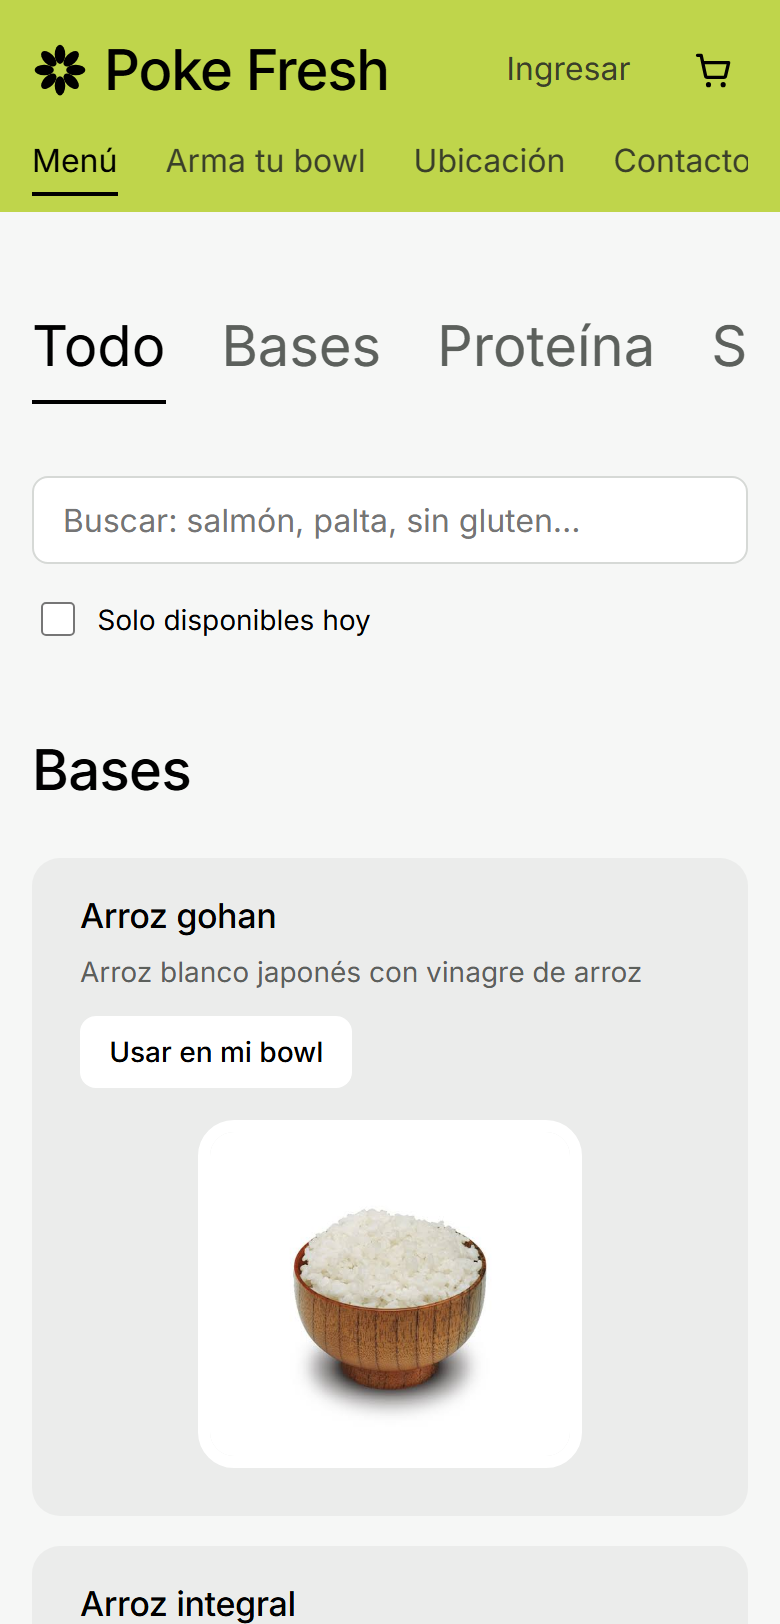
\includegraphics[width=\linewidth,height=0.4\textheight,keepaspectratio]{../evidencias/movil/02-menu.png}
\captionof{figure}{Menú}
\end{minipage}\hfill
\begin{minipage}[t]{0.242\linewidth}\centering
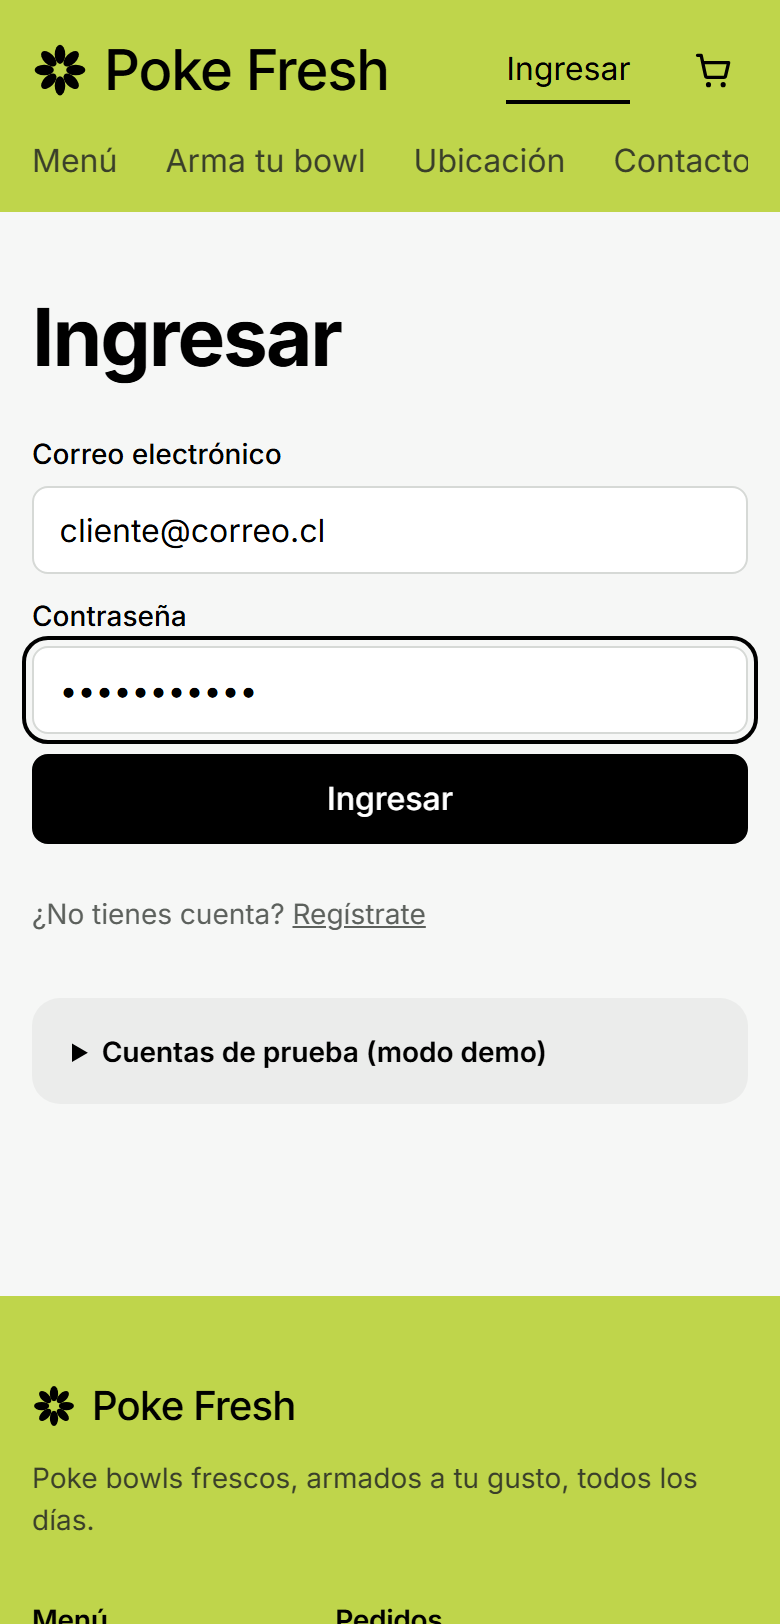
\includegraphics[width=\linewidth,height=0.4\textheight,keepaspectratio]{../evidencias/movil/03-ingreso.png}
\captionof{figure}{Ingreso}
\end{minipage}\hfill
\begin{minipage}[t]{0.242\linewidth}\centering
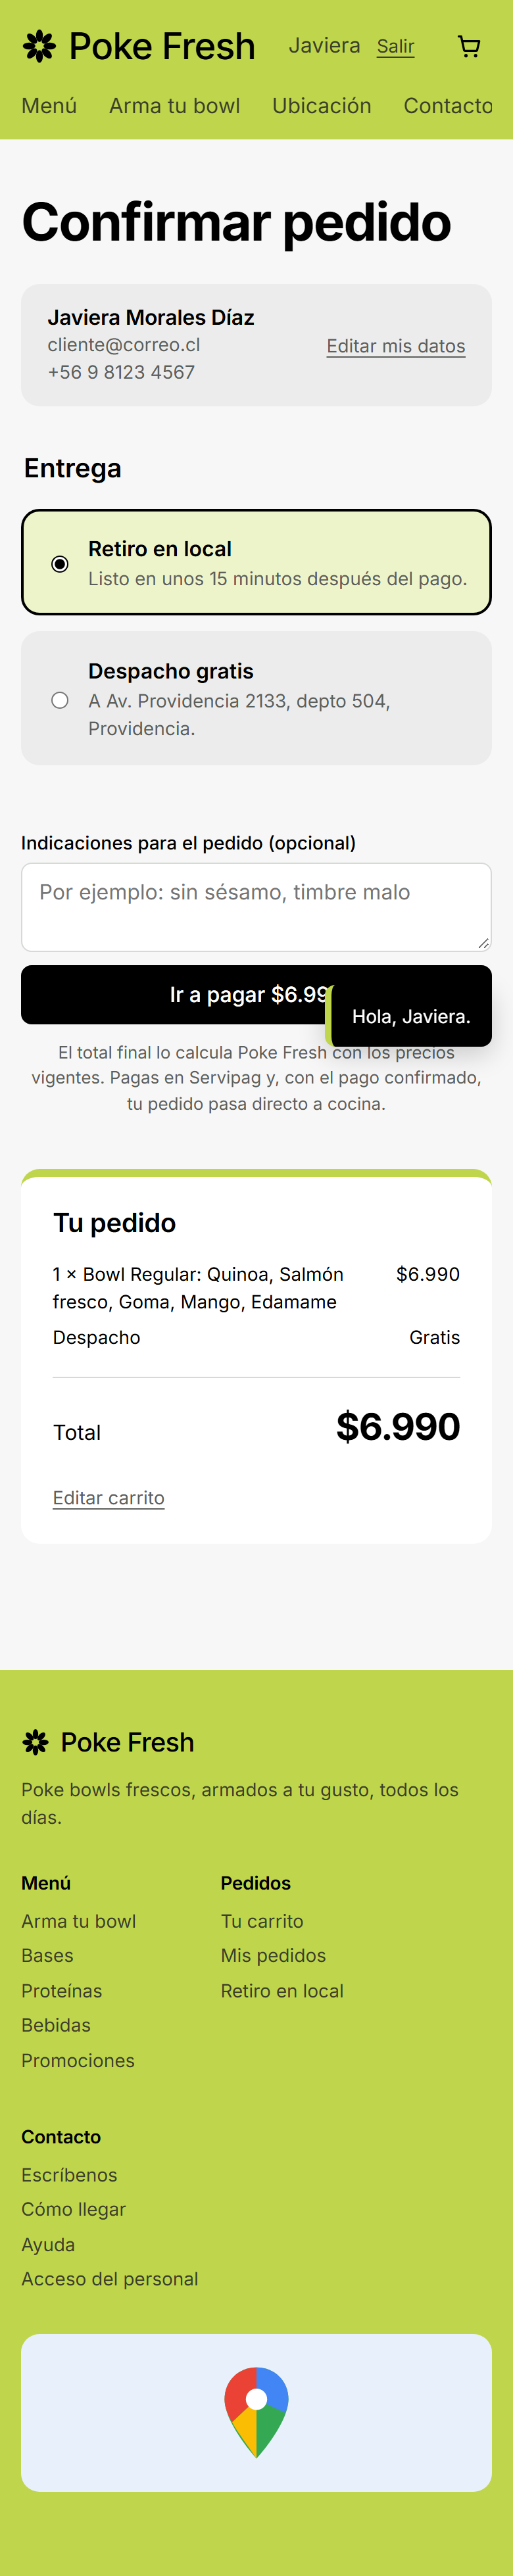
\includegraphics[width=\linewidth,height=0.4\textheight,keepaspectratio]{../evidencias/movil/04-checkout.png}
\captionof{figure}{Checkout}
\end{minipage}
\end{figure}

\begin{figure}[H]\centering
\begin{minipage}[t]{0.242\linewidth}\centering
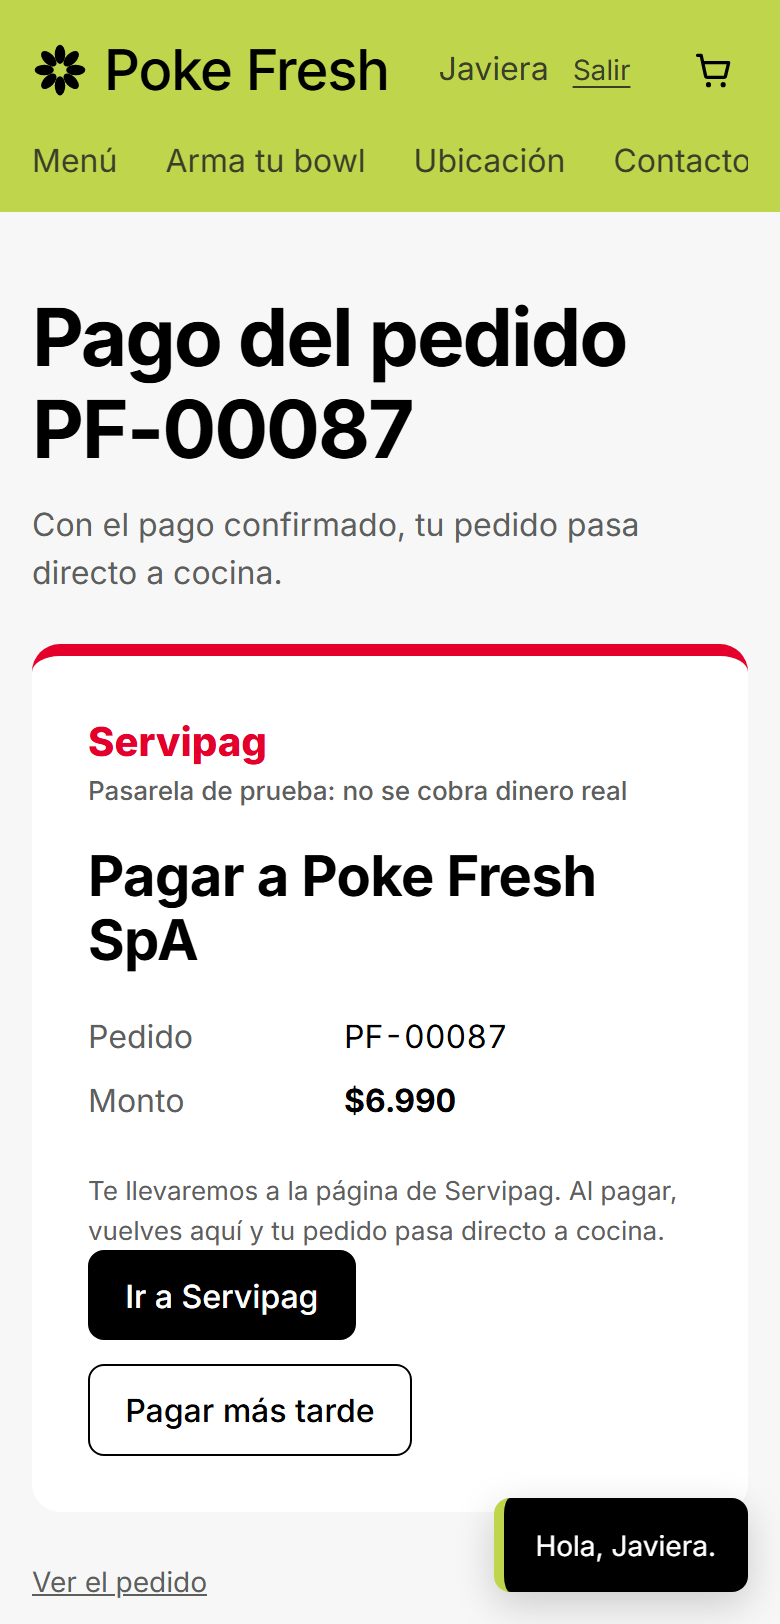
\includegraphics[width=\linewidth,height=0.4\textheight,keepaspectratio]{../evidencias/movil/05-pago.png}
\captionof{figure}{Pago}
\end{minipage}\hfill
\begin{minipage}[t]{0.242\linewidth}\centering
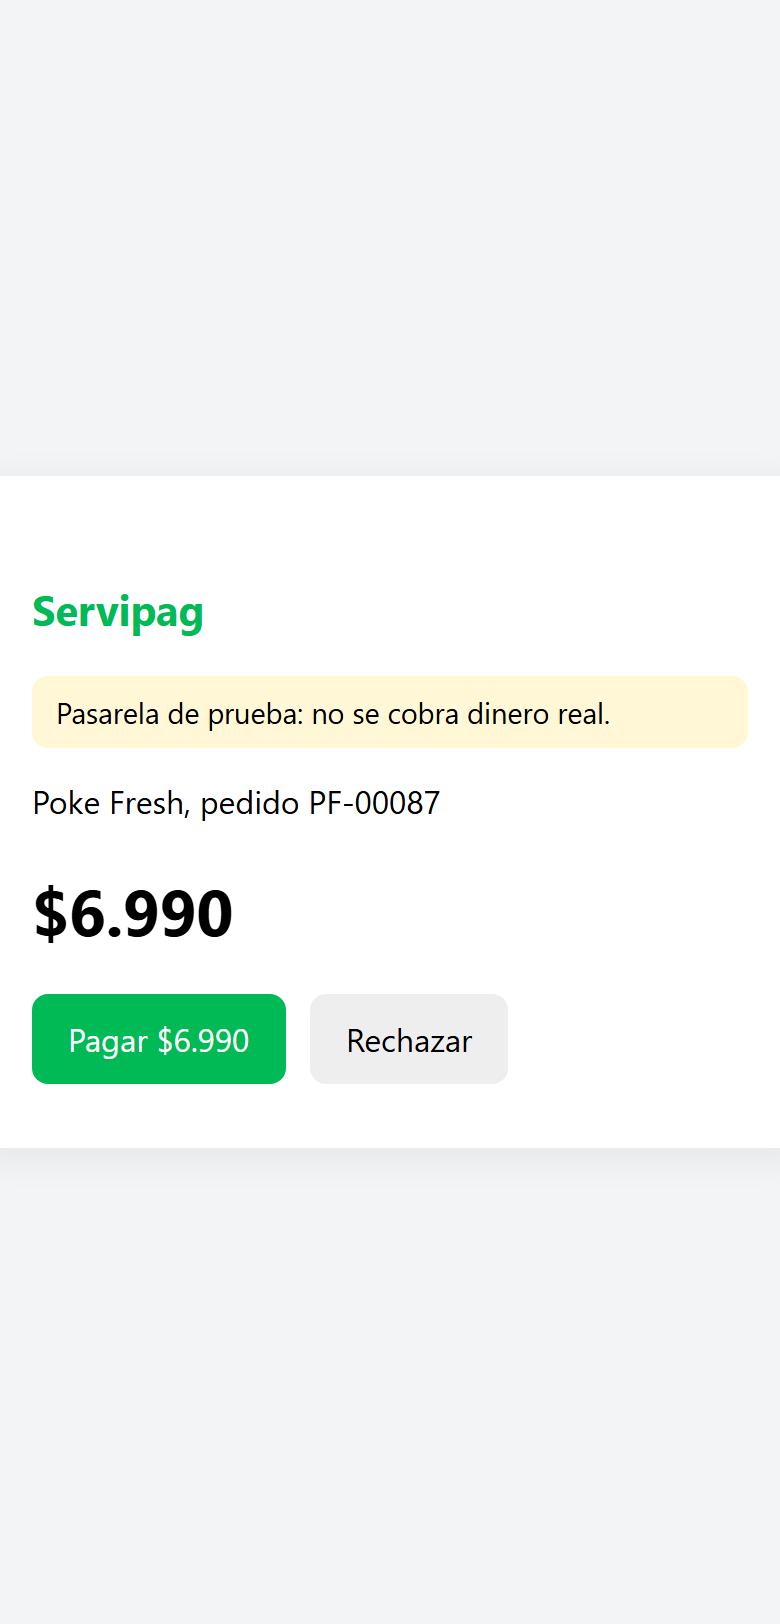
\includegraphics[width=\linewidth,height=0.4\textheight,keepaspectratio]{../evidencias/movil/06-pasarela-servipag.png}
\captionof{figure}{Pasarela Servipag}
\end{minipage}\hfill
\begin{minipage}[t]{0.242\linewidth}\centering
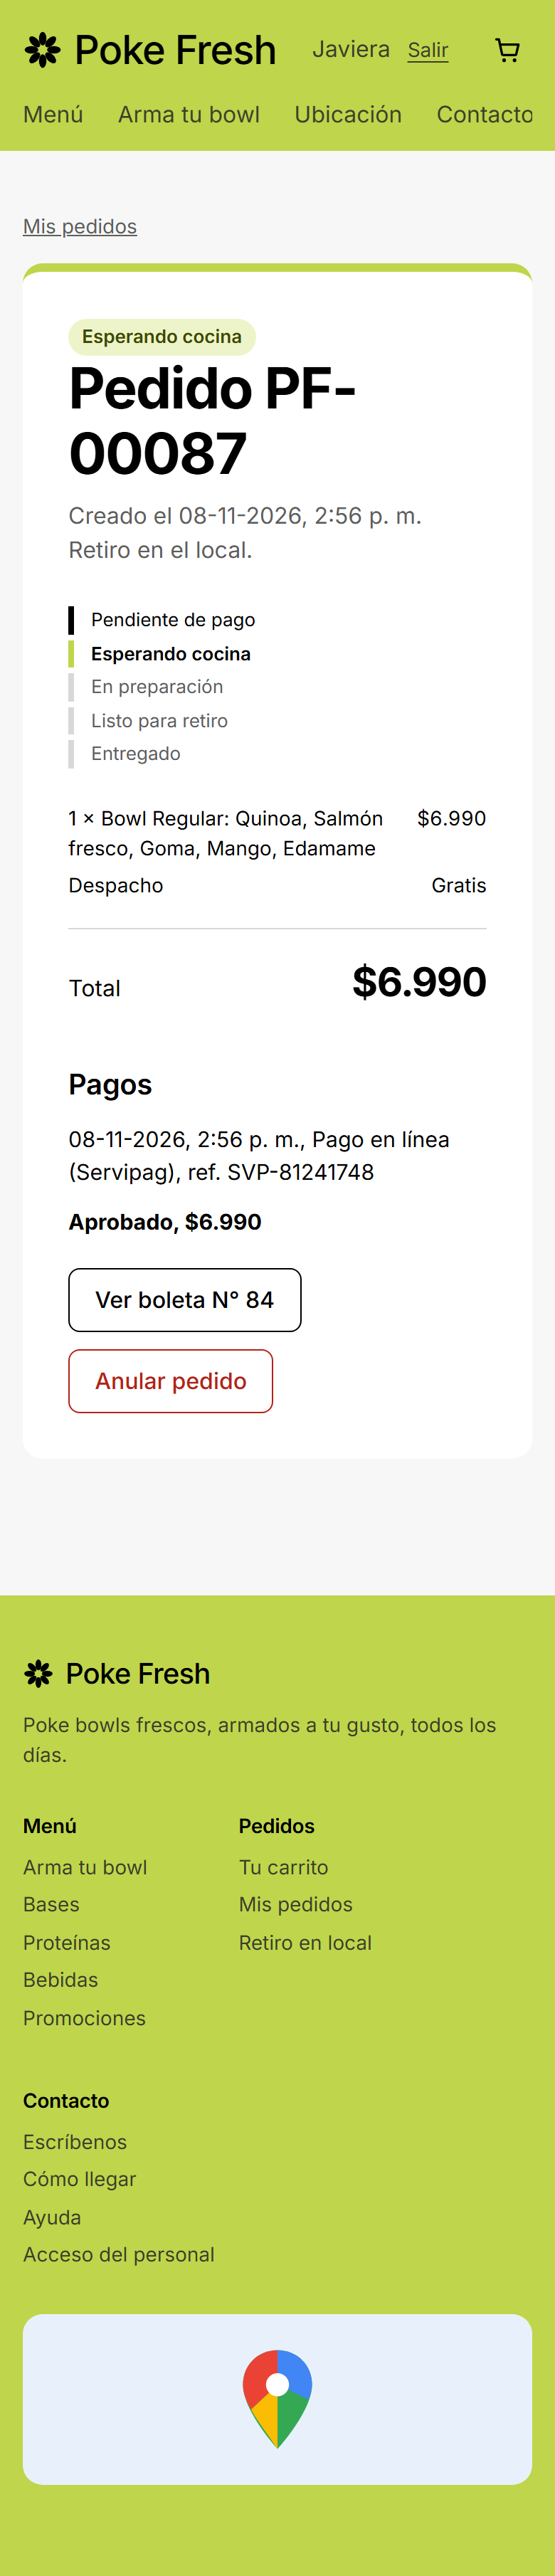
\includegraphics[width=\linewidth,height=0.4\textheight,keepaspectratio]{../evidencias/movil/07-pedido-pagado.png}
\captionof{figure}{Pedido pagado con boleta}
\end{minipage}\hfill
\begin{minipage}[t]{0.242\linewidth}\centering
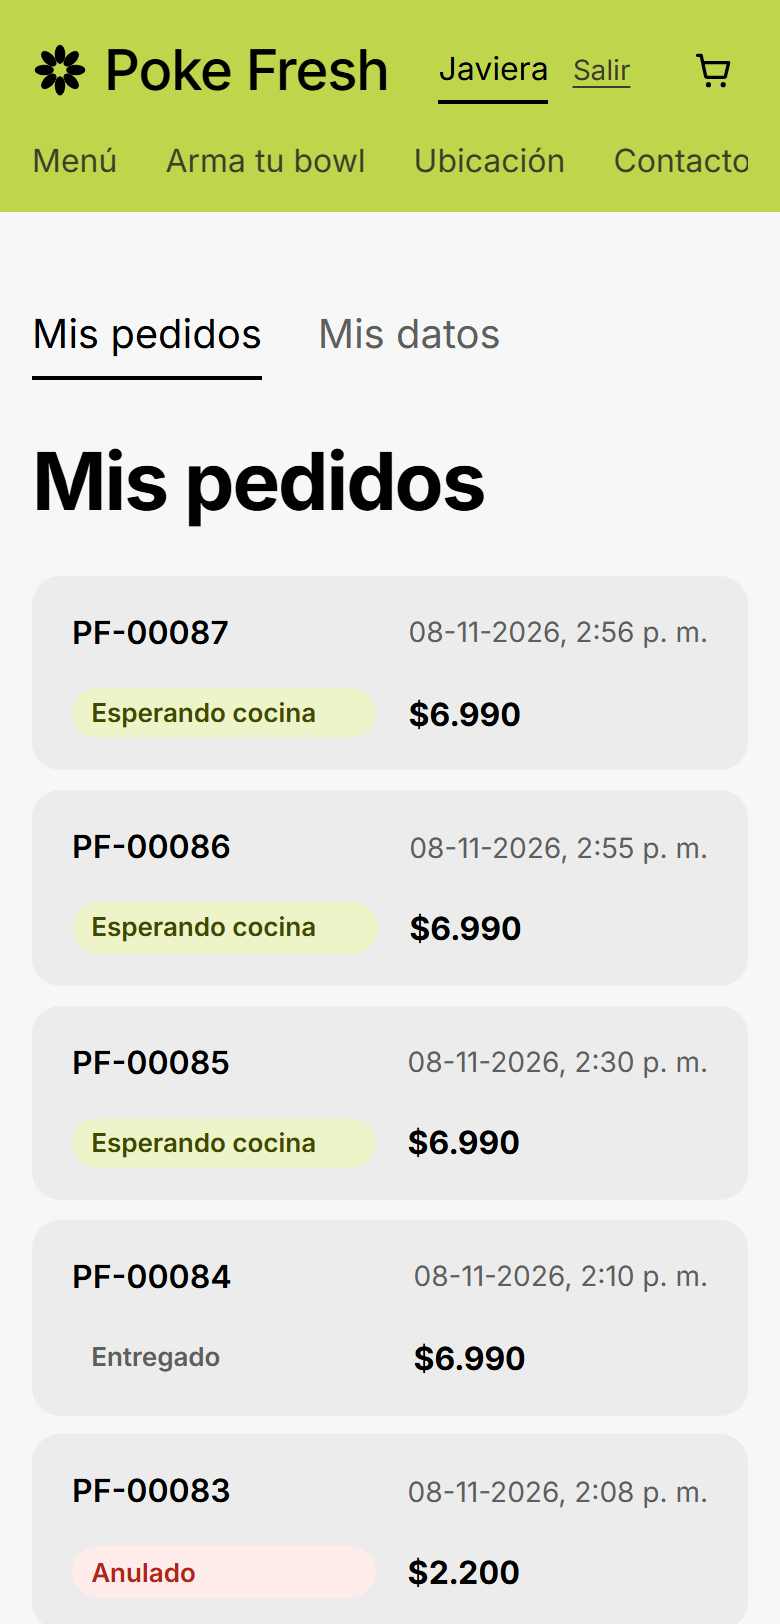
\includegraphics[width=\linewidth,height=0.4\textheight,keepaspectratio]{../evidencias/movil/08-mis-pedidos.png}
\captionof{figure}{Mis pedidos}
\end{minipage}
\end{figure}

Es una emulación en Chromium, no un teléfono real.


\subsubsection{Navegador real (Microsoft Edge): compra completa por HTTPS}

\begin{figure}[H]\centering
\begin{minipage}[t]{0.485\linewidth}\centering
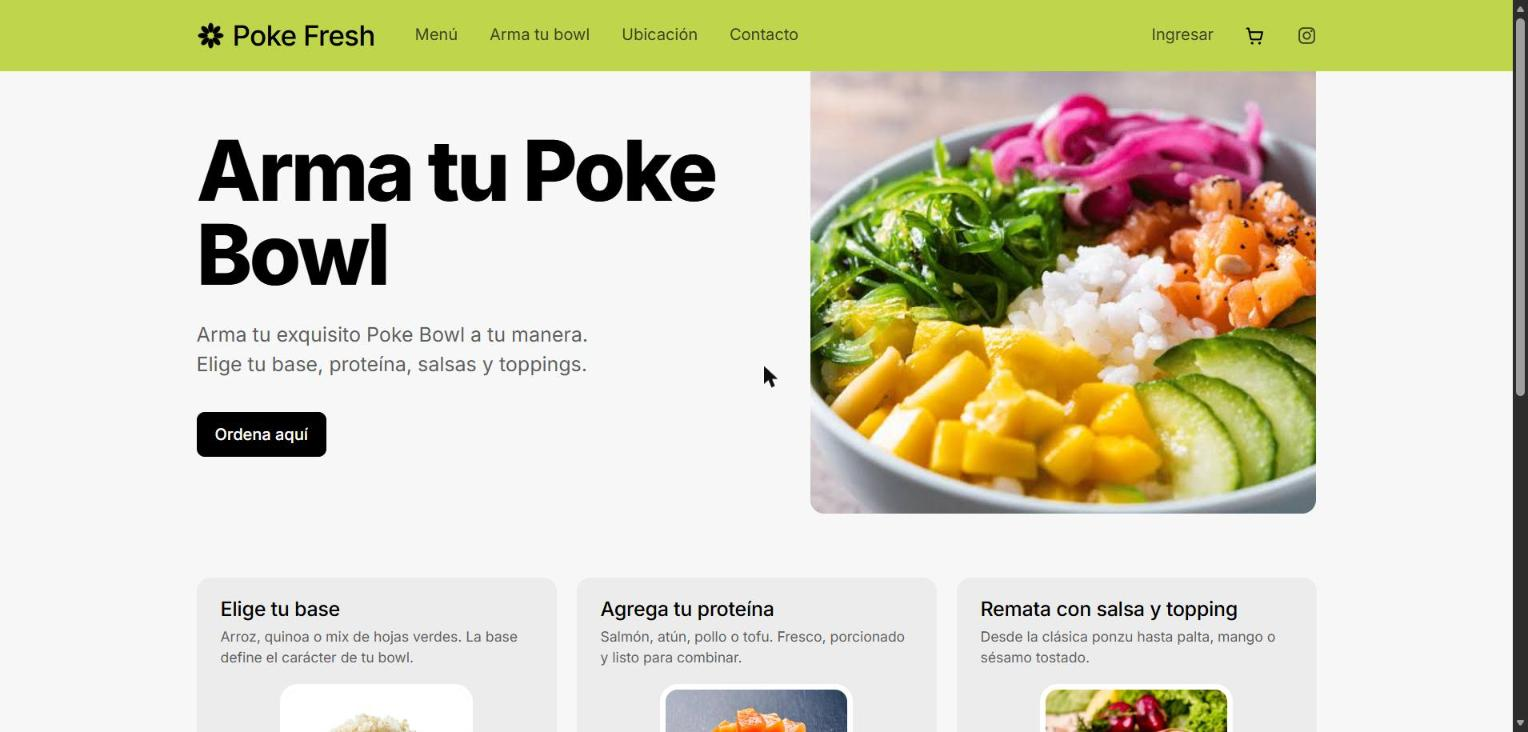
\includegraphics[width=\linewidth,height=0.42\textheight,keepaspectratio]{../evidencias/navegador-real/01-inicio.jpg}
\captionof{figure}{Inicio}
\end{minipage}\hfill
\begin{minipage}[t]{0.485\linewidth}\centering
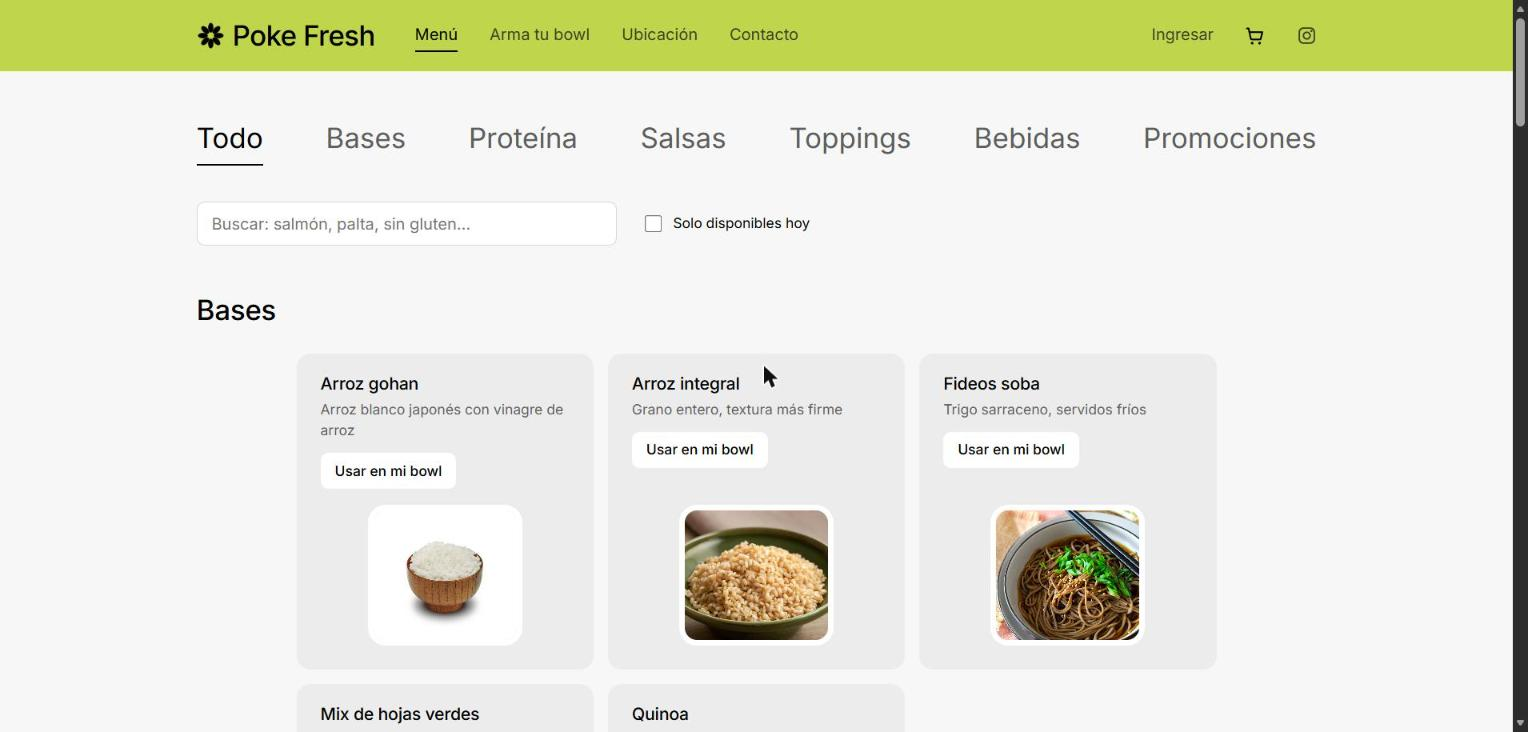
\includegraphics[width=\linewidth,height=0.42\textheight,keepaspectratio]{../evidencias/navegador-real/02-menu.jpg}
\captionof{figure}{Menú}
\end{minipage}
\end{figure}

\begin{figure}[H]\centering
\begin{minipage}[t]{0.485\linewidth}\centering
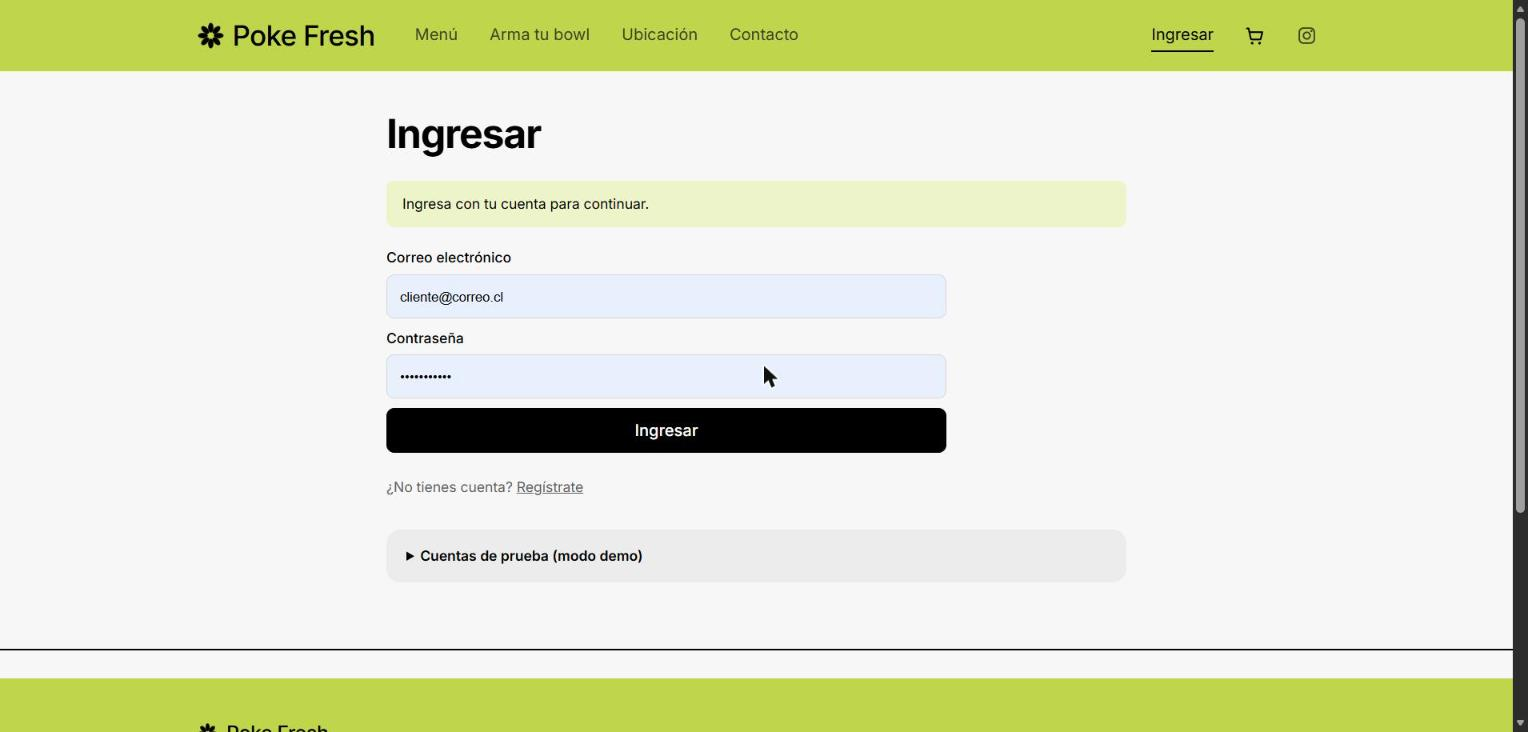
\includegraphics[width=\linewidth,height=0.42\textheight,keepaspectratio]{../evidencias/navegador-real/03-ingreso.jpg}
\captionof{figure}{Ingreso}
\end{minipage}\hfill
\begin{minipage}[t]{0.485\linewidth}\centering
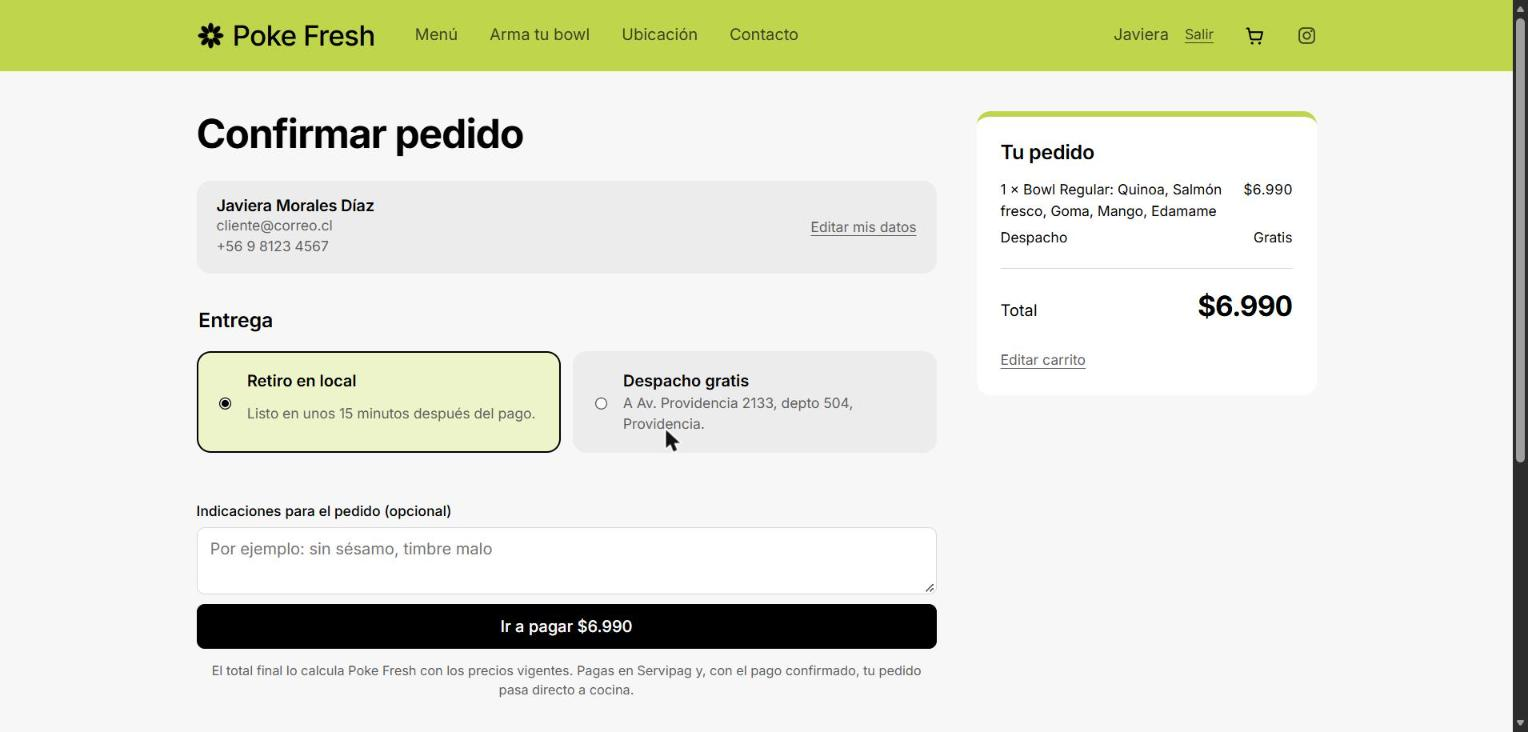
\includegraphics[width=\linewidth,height=0.42\textheight,keepaspectratio]{../evidencias/navegador-real/04-checkout.jpg}
\captionof{figure}{Checkout}
\end{minipage}
\end{figure}

\begin{figure}[H]\centering
\begin{minipage}[t]{0.485\linewidth}\centering
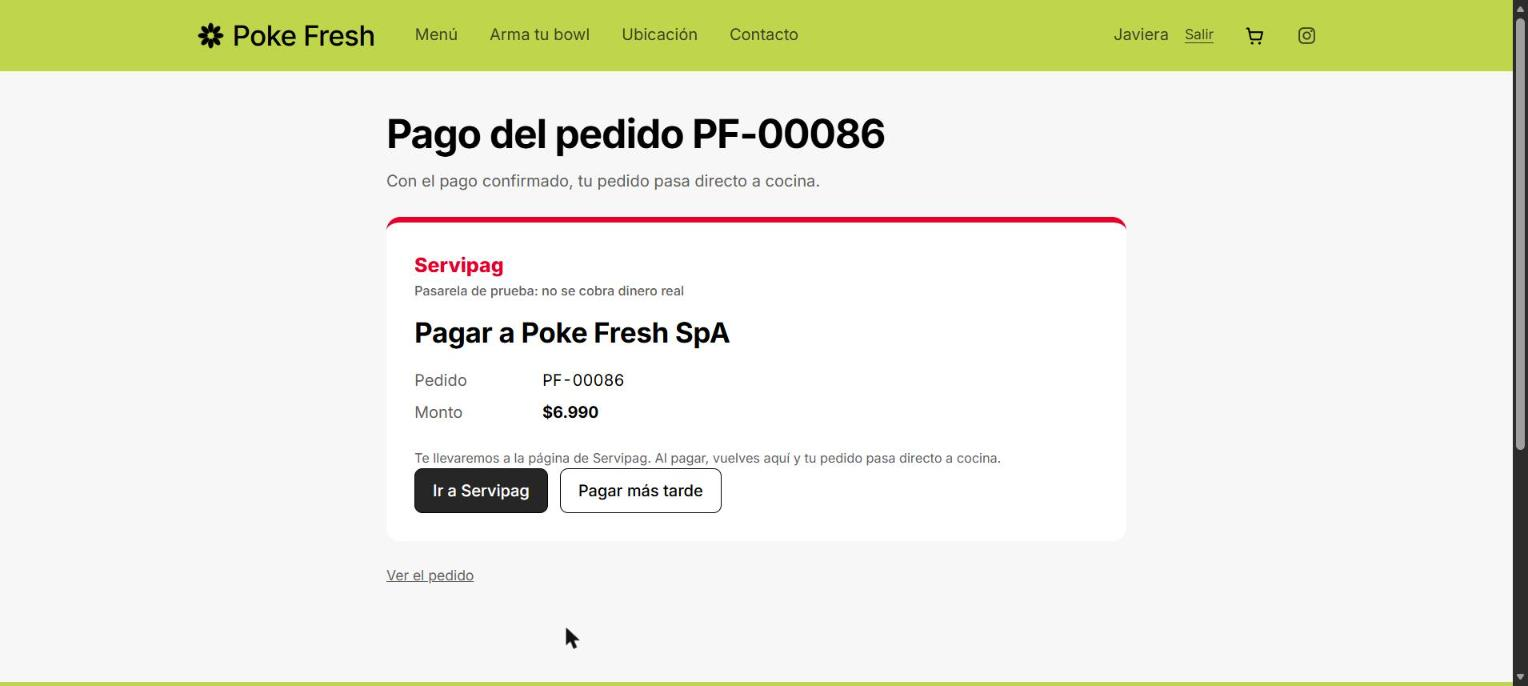
\includegraphics[width=\linewidth,height=0.42\textheight,keepaspectratio]{../evidencias/navegador-real/05-pago.jpg}
\captionof{figure}{Pago}
\end{minipage}\hfill
\begin{minipage}[t]{0.485\linewidth}\centering
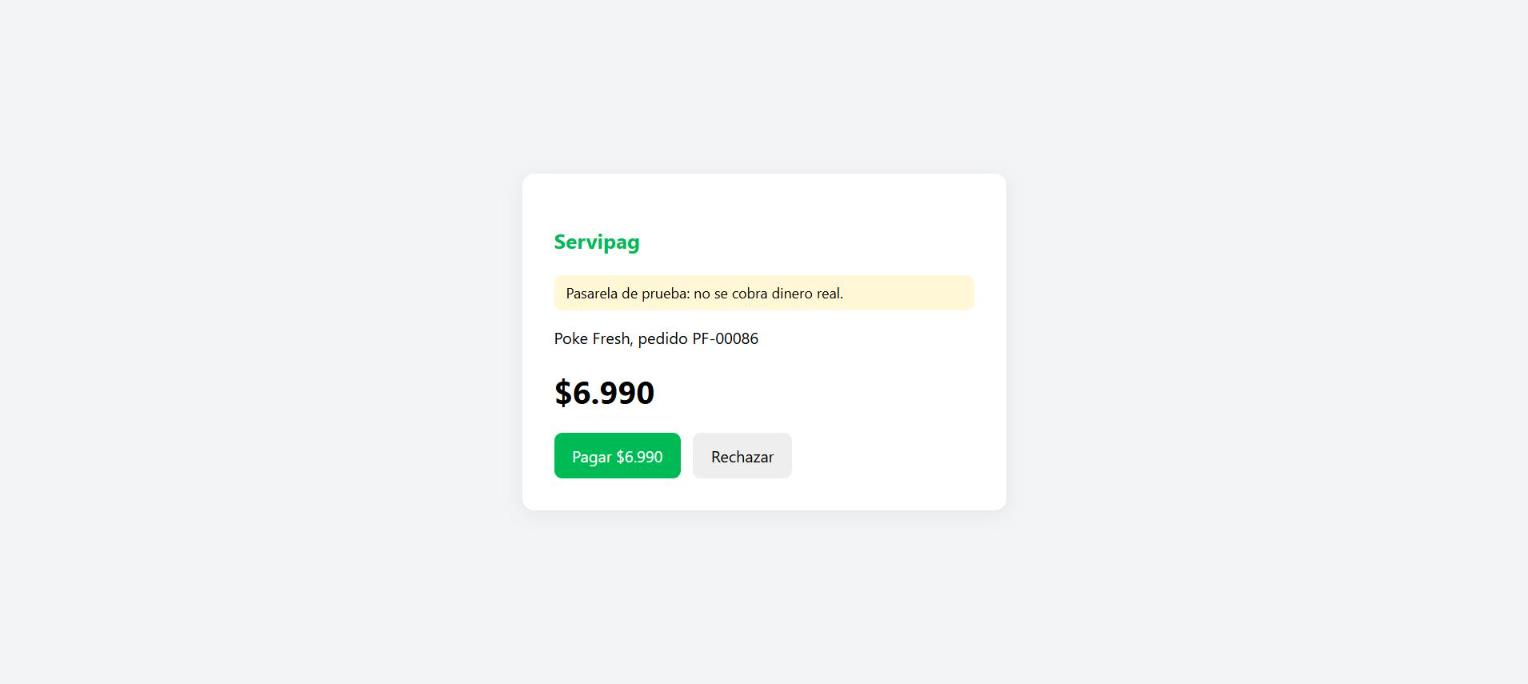
\includegraphics[width=\linewidth,height=0.42\textheight,keepaspectratio]{../evidencias/navegador-real/06-pasarela-servipag.jpg}
\captionof{figure}{Pasarela de pago en https://localhost:9000}
\end{minipage}
\end{figure}

\begin{figure}[H]\centering
\begin{minipage}[t]{0.485\linewidth}\centering
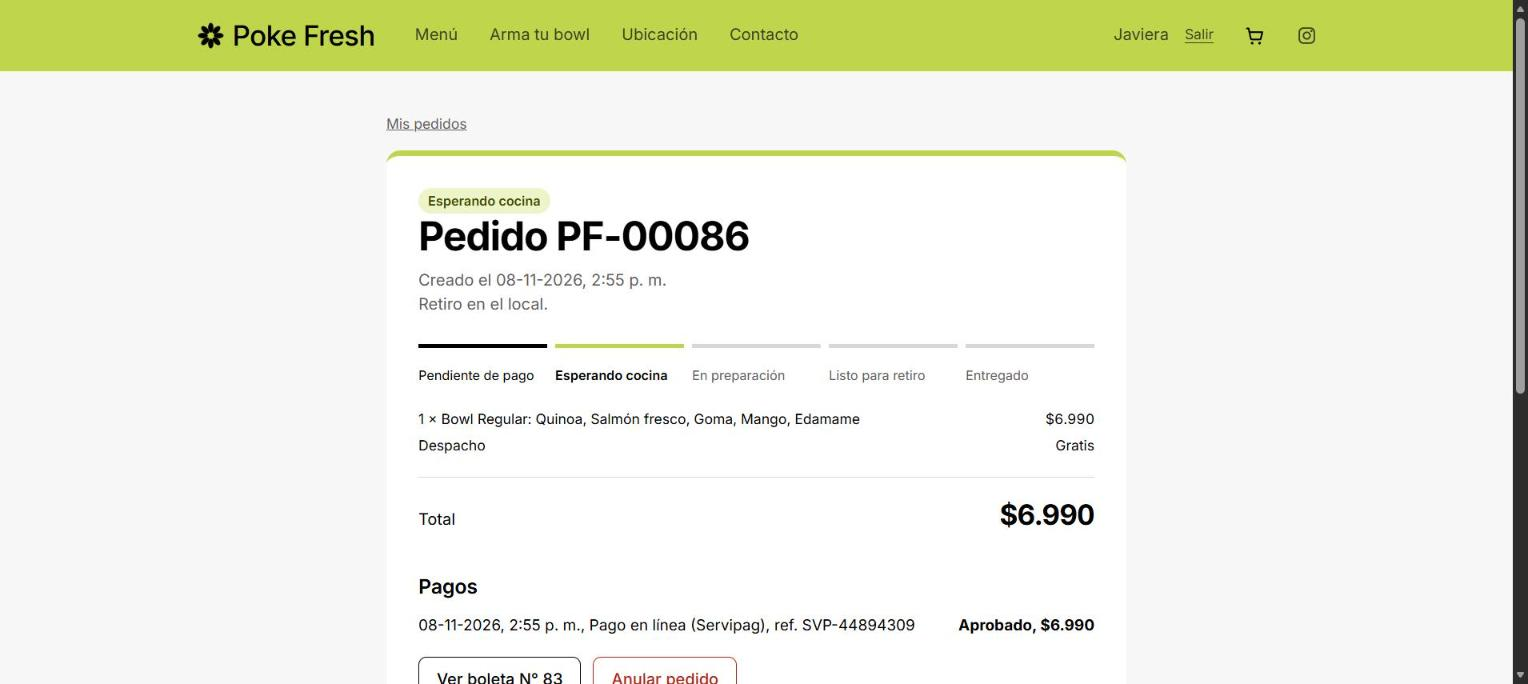
\includegraphics[width=\linewidth,height=0.42\textheight,keepaspectratio]{../evidencias/navegador-real/07-pedido-pagado.jpg}
\captionof{figure}{Pedido pagado}
\end{minipage}\hfill
\begin{minipage}[t]{0.485\linewidth}\centering
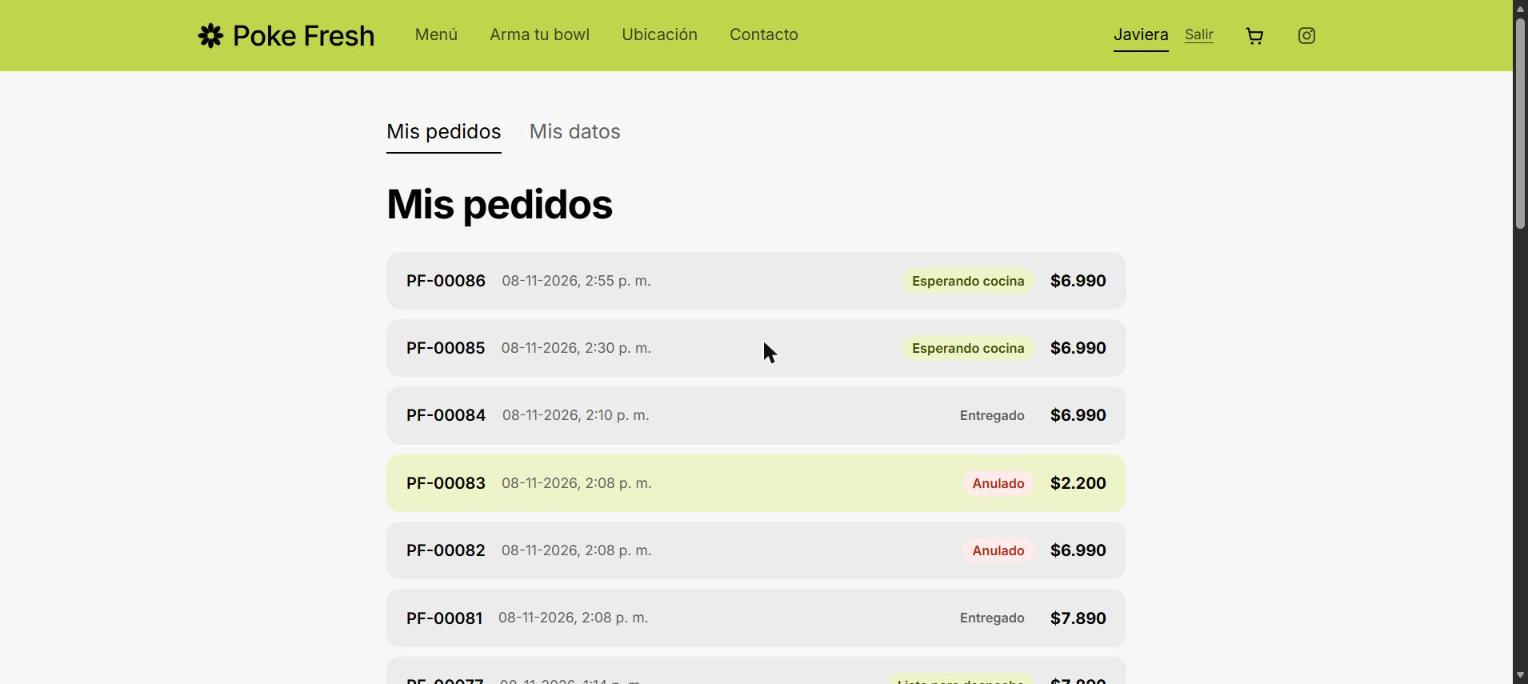
\includegraphics[width=\linewidth,height=0.42\textheight,keepaspectratio]{../evidencias/navegador-real/08-mis-pedidos.jpg}
\captionof{figure}{Mis pedidos}
\end{minipage}
\end{figure}

Las capturas muestran la página y no la barra de direcciones; el protocolo consta en \texttt{evidencias/\allowbreak{}navegador-\allowbreak{}real/\allowbreak{}datos-\allowbreak{}navegador.\allowbreak{}json}.


\subsection{Matriz requisito, pantalla, servicio, prueba y evidencia}

{\footnotesize
\setlength{\tabcolsep}{3pt}\renewcommand{\arraystretch}{1.15}
\begin{longtable}{|>{\raggedright\arraybackslash}p{\dimexpr 0.0611\linewidth-2\tabcolsep\relax}|>{\raggedright\arraybackslash}p{\dimexpr 0.1268\linewidth-2\tabcolsep\relax}|>{\raggedright\arraybackslash}p{\dimexpr 0.2599\linewidth-2\tabcolsep\relax}|>{\raggedright\arraybackslash}p{\dimexpr 0.2682\linewidth-2\tabcolsep\relax}|>{\raggedright\arraybackslash}p{\dimexpr 0.0988\linewidth-2\tabcolsep\relax}|>{\raggedright\arraybackslash}p{\dimexpr 0.1851\linewidth-2\tabcolsep\relax}|}
\hline
\textbf{Req.} & \textbf{Pantalla} & \textbf{Servicio} & \textbf{Prueba} & \textbf{Resultado} & \textbf{Evidencia} \\ \hline
\endfirsthead
\hline
\textbf{Req.} & \textbf{Pantalla} & \textbf{Servicio} & \textbf{Prueba} & \textbf{Resultado} & \textbf{Evidencia} \\ \hline
\endhead
R1 & Menú, Arma tu bowl & inventario (S01 a S03) & \texttt{test\_\allowbreak{}catalogo\_\allowbreak{}publico.\allowbreak{}.\allowbreak{}.\allowbreak{}}, \texttt{test\_\allowbreak{}cotizacion.\allowbreak{}.\allowbreak{}.\allowbreak{}}, caso 7.1 & OK & \texttt{pantallas/\allowbreak{}02-\allowbreak{}menu-\allowbreak{}desde-\allowbreak{}inventario.\allowbreak{}png} \\ \hline
R2 & Arma tu bowl & inventario (S03) & \texttt{test\_\allowbreak{}reglas\_\allowbreak{}de\_\allowbreak{}armado.\allowbreak{}.\allowbreak{}.\allowbreak{}}, caso 10.1 & OK & e2e 10.1 \\ \hline
R3 & Promo & inventario (S03) & \texttt{test\_\allowbreak{}crear\_\allowbreak{}pedido\_\allowbreak{}calcula\_\allowbreak{}total.\allowbreak{}.\allowbreak{}.\allowbreak{}} (cotizador de promos en \texttt{reglas.\allowbreak{}py}) & OK & — \\ \hline
R4 & Carrito & frontend + inventario (S03, S15) & recorrido de pantallas & OK & \texttt{pantallas/\allowbreak{}03-\allowbreak{}checkout.\allowbreak{}png} \\ \hline
R5 & Registro, Verificar & clientes + Auth (S07, S38, S39) & \texttt{test\_\allowbreak{}registro\_\allowbreak{}crea\_\allowbreak{}ficha.\allowbreak{}.\allowbreak{}.\allowbreak{}}, \texttt{cuenta nueva de cliente.\allowbreak{}.\allowbreak{}.\allowbreak{}} & OK & \texttt{pantallas/\allowbreak{}15-\allowbreak{}verificacion-\allowbreak{}correo.\allowbreak{}png}, \texttt{16-\allowbreak{}.\allowbreak{}.\allowbreak{}.\allowbreak{}} \\ \hline
R6 & Ingresar, Panel & Auth + gateway (S33 a S36, S40 a S43) & casos 7.3, 7.8, 7.11 & OK & e2e \\ \hline
R7 & Confirmar pedido & pedidos + clientes (S15) & \texttt{test\_\allowbreak{}despacho\_\allowbreak{}fuera\_\allowbreak{}de\_\allowbreak{}radio}, caso 10.1 & OK & e2e 10.1 \\ \hline
R8 & Pago, Pedido, Boleta & pagos + pasarela + pedidos + ActiveMQ (S27, S29, S18) & \texttt{test\_\allowbreak{}pago\_\allowbreak{}completo\_\allowbreak{}por\_\allowbreak{}la\_\allowbreak{}pasarela}, casos 7.6, 10.2, 10.3 & OK & \texttt{pantallas/\allowbreak{}04} a \texttt{06}; log del notificador \\ \hline
R9 & Cocina & pedidos (S16, S20, S21, S24) & \texttt{test\_\allowbreak{}flujo\_\allowbreak{}de\_\allowbreak{}cocina\_\allowbreak{}y\_\allowbreak{}despacho.\allowbreak{}.\allowbreak{}.\allowbreak{}}, caso 10.4 & OK & \texttt{pantallas/\allowbreak{}07-\allowbreak{}cocina.\allowbreak{}png} \\ \hline
R10 & Despacho & pedidos (S22, S23) & caso 10.4 & OK & \texttt{pantallas/\allowbreak{}08-\allowbreak{}despacho.\allowbreak{}png}, \texttt{09-\allowbreak{}.\allowbreak{}.\allowbreak{}.\allowbreak{}} \\ \hline
R11 & Pedido, Panel pedidos & pedidos + pagos + inventario (S25) & \texttt{test\_\allowbreak{}anular\_\allowbreak{}pedido\_\allowbreak{}pagado.\allowbreak{}.\allowbreak{}.\allowbreak{}}, \texttt{test\_\allowbreak{}no\_\allowbreak{}se\_\allowbreak{}anula.\allowbreak{}.\allowbreak{}.\allowbreak{}}, casos 10.5, 10.6 & OK & e2e \\ \hline
R12 & Productos, Clientes, Usuarios & inventario, clientes, Auth (S04 a S06, S10 a S14, S40 a S43) & \texttt{test\_\allowbreak{}solo\_\allowbreak{}admin\_\allowbreak{}elimina.\allowbreak{}.\allowbreak{}.\allowbreak{}}, \texttt{test\_\allowbreak{}admin\_\allowbreak{}registra\_\allowbreak{}en\_\allowbreak{}local.\allowbreak{}.\allowbreak{}.\allowbreak{}}, \texttt{solo un admin gestiona usuarios.\allowbreak{}.\allowbreak{}.\allowbreak{}} & OK & \texttt{pantallas/\allowbreak{}12}, \texttt{13} \\ \hline
R13 & Caja, Reportes & pedidos + GraphQL (S26, S32) & \texttt{test\_\allowbreak{}reporte\_\allowbreak{}de\_\allowbreak{}ventas.\allowbreak{}.\allowbreak{}.\allowbreak{}}, caso 8.3 & OK & \texttt{pantallas/\allowbreak{}11-\allowbreak{}reportes-\allowbreak{}graphql.\allowbreak{}png} \\ \hline
R14 & Pedido, Mis pedidos, Boleta & pedidos + GraphQL (S08, S09, S16 a S18, S30) & caso 7.5, 8.1 & OK & \texttt{pantallas/\allowbreak{}09}, \texttt{10} \\ \hline
\end{longtable}
}

\subsection{Ejemplo de autorización por pedido}

Con la misma regla (“un cliente solo ve sus pedidos”, aplicada por el servicio de pedidos):


\begin{itemize}[nosep,leftmargin=*]
\item \textbf{Autorizada:} la cliente \texttt{cli\_\allowbreak{}demo\_\allowbreak{}1} pide \texttt{GET /\allowbreak{}api/\allowbreak{}v1/\allowbreak{}pedidos/\allowbreak{}PF-\allowbreak{}00081} $\rightarrow$ \texttt{200} con su pedido.
\item \textbf{Denegada:} el cliente \texttt{cli\_\allowbreak{}demo\_\allowbreak{}2} pide lo mismo $\rightarrow$ \texttt{404 NO\_\allowbreak{}ENCONTRADO}, sin datos del pedido (no confirma ni que existe). Por GraphQL, \texttt{resumenPedido} responde \texttt{null}.
\end{itemize}

Ambas en el caso 7.5 (\texttt{evidencias/\allowbreak{}e2e-\allowbreak{}resultados.\allowbreak{}json}, con sus \texttt{X-\allowbreak{}Request-\allowbreak{}Id}, que se pueden buscar en \texttt{docker compose logs pedidos}).


\subsection{Operación}

\begin{itemize}[nosep,leftmargin=*]
\item \textbf{Iniciar y detener:} ver \texttt{README.\allowbreak{}md} (\texttt{docker compose up -\allowbreak{}d -\allowbreak{}-\allowbreak{}build}, \texttt{docker compose down}).
\item \textbf{Acceso:} \texttt{https:\allowbreak{}/\allowbreak{}/\allowbreak{}localhost:\allowbreak{}8080} (tienda y API) y \texttt{https:\allowbreak{}/\allowbreak{}/\allowbreak{}localhost:\allowbreak{}9000} (pasarela). Los certificados los firma una CA de prueba que crea \texttt{tls-\allowbreak{}init}, así que el navegador, o un antivirus que revise HTTPS, mostrará una advertencia en cada puerto; hay que aceptarla en ambos. Si otro programa ocupa el puerto 8080 en IPv4, hay que detenerlo (ver README).
\item \textbf{Configurar secretos:} solo \texttt{.\allowbreak{}env} con la clave raíz de Mongo; el resto lo crea \texttt{vault-\allowbreak{}init}. Para rotar un secreto: borrarlo en Vault y volver a correr \texttt{docker compose up -\allowbreak{}d} (excepto el pepper).
\item \textbf{Datos de prueba:} automáticos con \texttt{MODO\_\allowbreak{}DEMO=\allowbreak{}true} (servicio \texttt{semilla}).
\item \textbf{Health checks:} cada servicio tiene \texttt{/\allowbreak{}salud} (estado de Mongo y Vault), usado por Docker; \texttt{GET /\allowbreak{}api/\allowbreak{}salud} reúne todos.
\item \textbf{Logs:} una línea por petición con método, ruta, estado, duración, rol y \texttt{X-\allowbreak{}Request-\allowbreak{}Id}; sin cuerpos, correos ni tokens.
\item \textbf{Dependencias versionadas:} \texttt{package-\allowbreak{}lock.\allowbreak{}json} en cada proyecto Node, versiones fijas en \texttt{servicios/\allowbreak{}requirements.\allowbreak{}txt}, imágenes con versión (\texttt{mongo:\allowbreak{}7.\allowbreak{}0}, \texttt{hashicorp/\allowbreak{}vault:\allowbreak{}1.\allowbreak{}18}, \texttt{apache/\allowbreak{}activemq-\allowbreak{}classic:\allowbreak{}6.\allowbreak{}1.\allowbreak{}4}).
\end{itemize}

\clearpage
% Generado desde docs/INFORME.md. Editar libremente.

\section{Anexo A. Ejemplos de contrato por operación}

La sección 1 muestra el ejemplo completo de S01, S07, S15, S20, S22, S25, S27, S29 y S33. Este anexo agrega uno para cada operación restante, de modo que las 44 tienen petición y respuesta con datos ficticios. En todos, los errores tienen la forma \texttt{\{"codigo":\allowbreak{} ".\allowbreak{}.\allowbreak{}.\allowbreak{}",\allowbreak{} "mensaje":\allowbreak{} ".\allowbreak{}.\allowbreak{}.\allowbreak{}",\allowbreak{} "idPeticion":\allowbreak{} ".\allowbreak{}.\allowbreak{}.\allowbreak{}"\}} y los códigos de la matriz del módulo 1. Se abrevian con \texttt{.\allowbreak{}.\allowbreak{}.\allowbreak{}} los campos que ya se mostraron en otro ejemplo. S30 (\texttt{resumenPedido}) tiene su consulta y su respuesta completas en la sección 8.


\subsection{Catálogo (inventario)}

\textbf{S02, obtener un producto} (anónimo).


\begin{codigo}
GET /\allowbreak{}api/\allowbreak{}v1/\allowbreak{}catalogo/\allowbreak{}items/\allowbreak{}pro\_\allowbreak{}atun\par
\end{codigo}

\begin{codigo}
200 \{"id":\allowbreak{} "pro\_\allowbreak{}atun",\allowbreak{} "categoria":\allowbreak{} "PROTEINA",\allowbreak{} "nombre":\allowbreak{} "Atún",\allowbreak{} "descripcion":\allowbreak{} "Grado sashimi,\allowbreak{} corte del día",\allowbreak{} "precio":\allowbreak{} 1500,\allowbreak{} "disponible":\allowbreak{} true\}\par
404 \{"codigo":\allowbreak{} "NO\_\allowbreak{}ENCONTRADO",\allowbreak{} "mensaje":\allowbreak{} "No existe el item pro\_\allowbreak{}zzz.\allowbreak{}",\allowbreak{} "idPeticion":\allowbreak{} "e2e-\allowbreak{}4c1d9a0b7e2f"\}\par
\end{codigo}

\textbf{S03, reglas del armado} (anónimo).


\begin{codigo}
GET /\allowbreak{}api/\allowbreak{}v1/\allowbreak{}catalogo/\allowbreak{}configuracion\par
\end{codigo}

\begin{codigo}
200 \{"tamanos":\allowbreak{} [\allowbreak{}\{"id":\allowbreak{} "regular",\allowbreak{} "nombre":\allowbreak{} "Regular",\allowbreak{} "descripcion":\allowbreak{} "Porción individual",\allowbreak{} "precio":\allowbreak{} 6990,\allowbreak{} "salsasIncluidas":\allowbreak{} 2,\allowbreak{} "toppingsIncluidos":\allowbreak{} 3\},\allowbreak{} .\allowbreak{}.\allowbreak{}.\allowbreak{}],\allowbreak{}\par
\hspace*{5\ttw}"reglas":\allowbreak{} \{"basesIncluidas":\allowbreak{} 1,\allowbreak{} "maxBases":\allowbreak{} 3,\allowbreak{} "recargoBaseExtra":\allowbreak{} 500,\allowbreak{} "proteinasIncluidas":\allowbreak{} 1,\allowbreak{} "maxProteinas":\allowbreak{} 3,\allowbreak{} "recargoProteinaExtra":\allowbreak{} 2500,\allowbreak{} .\allowbreak{}.\allowbreak{}.\allowbreak{}\},\allowbreak{}\par
\hspace*{5\ttw}"promos":\allowbreak{} \{"promo\_\allowbreak{}combo":\allowbreak{} \{"bowls":\allowbreak{} 1,\allowbreak{} "bebida":\allowbreak{} true,\allowbreak{} "tamanoId":\allowbreak{} "regular",\allowbreak{} "detalle":\allowbreak{} "Arma tu bowl regular y elige tu bebida.\allowbreak{}"\},\allowbreak{} .\allowbreak{}.\allowbreak{}.\allowbreak{}\}\}\par
\end{codigo}

\textbf{S04, crear un producto} (admin o dueño). Con rol de administración la respuesta incluye \texttt{stock} y \texttt{activo}.


\begin{codigo}
POST /\allowbreak{}api/\allowbreak{}v1/\allowbreak{}catalogo/\allowbreak{}items\par
\{"categoria":\allowbreak{} "TOPPING",\allowbreak{} "nombre":\allowbreak{} "Cebolla crispy",\allowbreak{} "descripcion":\allowbreak{} "Crocante,\allowbreak{} para dar textura",\allowbreak{} "precio":\allowbreak{} 700,\allowbreak{} "stock":\allowbreak{} 50,\allowbreak{} "disponible":\allowbreak{} true\}\par
\end{codigo}

\begin{codigo}
201 \{"id":\allowbreak{} "top\_\allowbreak{}cebolla\_\allowbreak{}crispy",\allowbreak{} "categoria":\allowbreak{} "TOPPING",\allowbreak{} "nombre":\allowbreak{} "Cebolla crispy",\allowbreak{} "descripcion":\allowbreak{} "Crocante,\allowbreak{} para dar textura",\allowbreak{} "precio":\allowbreak{} 700,\allowbreak{} "disponible":\allowbreak{} true,\allowbreak{} "stock":\allowbreak{} 50,\allowbreak{} "activo":\allowbreak{} true\}\par
409 \{"codigo":\allowbreak{} "DUPLICADO",\allowbreak{} "mensaje":\allowbreak{} "Ya existe un item llamado \textbackslash{}"Cebolla crispy\textbackslash{}".\allowbreak{}",\allowbreak{} "idPeticion":\allowbreak{} ".\allowbreak{}.\allowbreak{}.\allowbreak{}"\}\par
\end{codigo}

\textbf{S05, modificar un producto} (admin o dueño). Solo se mandan los campos que cambian.


\begin{codigo}
PUT /\allowbreak{}api/\allowbreak{}v1/\allowbreak{}catalogo/\allowbreak{}items/\allowbreak{}top\_\allowbreak{}cebolla\_\allowbreak{}crispy\par
\{"precio":\allowbreak{} 800,\allowbreak{} "stock":\allowbreak{} 40\}\par
\end{codigo}

\begin{codigo}
200 \{"id":\allowbreak{} "top\_\allowbreak{}cebolla\_\allowbreak{}crispy",\allowbreak{} "categoria":\allowbreak{} "TOPPING",\allowbreak{} "nombre":\allowbreak{} "Cebolla crispy",\allowbreak{} .\allowbreak{}.\allowbreak{}.\allowbreak{},\allowbreak{} "precio":\allowbreak{} 800,\allowbreak{} "disponible":\allowbreak{} true,\allowbreak{} "stock":\allowbreak{} 40,\allowbreak{} "activo":\allowbreak{} true\}\par
\end{codigo}

\textbf{S06, eliminar un producto} (solo admin).


\begin{codigo}
DELETE /\allowbreak{}api/\allowbreak{}v1/\allowbreak{}catalogo/\allowbreak{}items/\allowbreak{}top\_\allowbreak{}cebolla\_\allowbreak{}crispy\par
\end{codigo}

\begin{codigo}
204 (\allowbreak{}sin cuerpo)\par
403 \{"codigo":\allowbreak{} "PROHIBIDO",\allowbreak{} "mensaje":\allowbreak{} "Tu perfil no tiene permiso para esta operación.\allowbreak{}",\allowbreak{} "idPeticion":\allowbreak{} ".\allowbreak{}.\allowbreak{}.\allowbreak{}"\}   (\allowbreak{}si es dueño)\par
\end{codigo}

\subsection{Clientes}

\textbf{S08, ver la ficha propia} (cliente).


\begin{codigo}
GET /\allowbreak{}api/\allowbreak{}v1/\allowbreak{}clientes/\allowbreak{}yo\par
\end{codigo}

\begin{codigo}
200 \{"id":\allowbreak{} "cli\_\allowbreak{}3fa9c01b22de",\allowbreak{} "run":\allowbreak{} "12345678-\allowbreak{}5",\allowbreak{} "nombre":\allowbreak{} "Ana Prueba Soto",\allowbreak{} "direccion":\allowbreak{} "Av.\allowbreak{} Italia 1500",\allowbreak{} "region":\allowbreak{} "Región Metropolitana de Santiago",\allowbreak{} "provincia":\allowbreak{} "Santiago",\allowbreak{} "comuna":\allowbreak{} "Ñuñoa",\allowbreak{} "fechaNacimiento":\allowbreak{} "1995-\allowbreak{}03-\allowbreak{}10",\allowbreak{} "sexo":\allowbreak{} "F",\allowbreak{} "email":\allowbreak{} "ana.\allowbreak{}prueba@correo.\allowbreak{}cl",\allowbreak{} "telefono":\allowbreak{} "+56 9 1111 2222",\allowbreak{} "activo":\allowbreak{} true,\allowbreak{} "origen":\allowbreak{} "WEB",\allowbreak{} "creadoEn":\allowbreak{} "2026-\allowbreak{}11-\allowbreak{}08T14:\allowbreak{}02:\allowbreak{}11.\allowbreak{}000Z",\allowbreak{} "tieneDespacho":\allowbreak{} true\}\par
\end{codigo}

\textbf{S09, editar la ficha propia} (cliente). El \texttt{run} y el \texttt{origen} no se pueden cambiar.


\begin{codigo}
PUT /\allowbreak{}api/\allowbreak{}v1/\allowbreak{}clientes/\allowbreak{}yo\par
\{"direccion":\allowbreak{} "Av.\allowbreak{} Italia 1520",\allowbreak{} "telefono":\allowbreak{} "+56 9 1111 3333"\}\par
\end{codigo}

\begin{codigo}
200 \{"id":\allowbreak{} "cli\_\allowbreak{}3fa9c01b22de",\allowbreak{} .\allowbreak{}.\allowbreak{}.\allowbreak{},\allowbreak{} "direccion":\allowbreak{} "Av.\allowbreak{} Italia 1520",\allowbreak{} "telefono":\allowbreak{} "+56 9 1111 3333",\allowbreak{} .\allowbreak{}.\allowbreak{}.\allowbreak{}\}\par
\end{codigo}

\textbf{S10, listar y buscar clientes} (admin).


\begin{codigo}
GET /\allowbreak{}api/\allowbreak{}v1/\allowbreak{}clientes?\allowbreak{}q=\allowbreak{}ana\par
\end{codigo}

\begin{codigo}
200 [\allowbreak{}\{"id":\allowbreak{} "cli\_\allowbreak{}3fa9c01b22de",\allowbreak{} "run":\allowbreak{} "12345678-\allowbreak{}5",\allowbreak{} "nombre":\allowbreak{} "Ana Prueba Soto",\allowbreak{} "direccion":\allowbreak{} "Av.\allowbreak{} Italia 1500",\allowbreak{} "region":\allowbreak{} "Región Metropolitana de Santiago",\allowbreak{} "provincia":\allowbreak{} "Santiago",\allowbreak{} "comuna":\allowbreak{} "Ñuñoa",\allowbreak{} "fechaNacimiento":\allowbreak{} "1995-\allowbreak{}03-\allowbreak{}10",\allowbreak{} "sexo":\allowbreak{} "F",\allowbreak{} "email":\allowbreak{} "ana.\allowbreak{}prueba@correo.\allowbreak{}cl",\allowbreak{} "telefono":\allowbreak{} "+56 9 1111 2222",\allowbreak{} "activo":\allowbreak{} true,\allowbreak{} "origen":\allowbreak{} "WEB",\allowbreak{} "creadoEn":\allowbreak{} "2026-\allowbreak{}11-\allowbreak{}08T14:\allowbreak{}02:\allowbreak{}11.\allowbreak{}000Z",\allowbreak{} "tieneDespacho":\allowbreak{} true,\allowbreak{} "emailVerificado":\allowbreak{} true\}]\par
\end{codigo}

\textbf{S11, registrar un cliente en el local} (admin). La clave temporal se entrega una sola vez y solo en modo demo.


\begin{codigo}
POST /\allowbreak{}api/\allowbreak{}v1/\allowbreak{}clientes\par
\{"run":\allowbreak{} "9.\allowbreak{}876.\allowbreak{}543-\allowbreak{}3",\allowbreak{} "nombre":\allowbreak{} "Luis Prueba Rojas",\allowbreak{} "direccion":\allowbreak{} "Av.\allowbreak{} Providencia 100",\allowbreak{} "region":\allowbreak{} "Región Metropolitana de Santiago",\allowbreak{} "provincia":\allowbreak{} "Santiago",\allowbreak{} "comuna":\allowbreak{} "Providencia",\allowbreak{} "fechaNacimiento":\allowbreak{} "1988-\allowbreak{}07-\allowbreak{}21",\allowbreak{} "sexo":\allowbreak{} "M",\allowbreak{} "email":\allowbreak{} "luis.\allowbreak{}prueba@correo.\allowbreak{}cl",\allowbreak{} "telefono":\allowbreak{} "+56 9 2222 3333"\}\par
\end{codigo}

\begin{codigo}
201 \{"cliente":\allowbreak{} \{"id":\allowbreak{} "cli\_\allowbreak{}7be41c0d93aa",\allowbreak{} "run":\allowbreak{} "9876543-\allowbreak{}3",\allowbreak{} "nombre":\allowbreak{} "Luis Prueba Rojas",\allowbreak{} .\allowbreak{}.\allowbreak{}.\allowbreak{},\allowbreak{} "origen":\allowbreak{} "ADMIN",\allowbreak{} "emailVerificado":\allowbreak{} false\},\allowbreak{} "claveTemporal":\allowbreak{} "kmpa4821"\}\par
\end{codigo}

\textbf{S12, abrir una ficha} (admin).


\begin{codigo}
GET /\allowbreak{}api/\allowbreak{}v1/\allowbreak{}clientes/\allowbreak{}cli\_\allowbreak{}3fa9c01b22de\par
\end{codigo}

\begin{codigo}
200 \{"id":\allowbreak{} "cli\_\allowbreak{}3fa9c01b22de",\allowbreak{} "run":\allowbreak{} "12345678-\allowbreak{}5",\allowbreak{} "nombre":\allowbreak{} "Ana Prueba Soto",\allowbreak{} "direccion":\allowbreak{} "Av.\allowbreak{} Italia 1500",\allowbreak{} "region":\allowbreak{} "Región Metropolitana de Santiago",\allowbreak{} "provincia":\allowbreak{} "Santiago",\allowbreak{} "comuna":\allowbreak{} "Ñuñoa",\allowbreak{} "fechaNacimiento":\allowbreak{} "1995-\allowbreak{}03-\allowbreak{}10",\allowbreak{} "sexo":\allowbreak{} "F",\allowbreak{} "email":\allowbreak{} "ana.\allowbreak{}prueba@correo.\allowbreak{}cl",\allowbreak{} "telefono":\allowbreak{} "+56 9 1111 2222",\allowbreak{} "activo":\allowbreak{} true,\allowbreak{} "origen":\allowbreak{} "WEB",\allowbreak{} "creadoEn":\allowbreak{} "2026-\allowbreak{}11-\allowbreak{}08T14:\allowbreak{}02:\allowbreak{}11.\allowbreak{}000Z",\allowbreak{} "tieneDespacho":\allowbreak{} true\}\par
404 \{"codigo":\allowbreak{} "NO\_\allowbreak{}ENCONTRADO",\allowbreak{} "mensaje":\allowbreak{} "No existe ese cliente.\allowbreak{}",\allowbreak{} "idPeticion":\allowbreak{} ".\allowbreak{}.\allowbreak{}.\allowbreak{}"\}\par
\end{codigo}

\textbf{S13, editar una ficha} (admin).


\begin{codigo}
PUT /\allowbreak{}api/\allowbreak{}v1/\allowbreak{}clientes/\allowbreak{}cli\_\allowbreak{}3fa9c01b22de\par
\{"telefono":\allowbreak{} "+56 9 7000 1111"\}\par
\end{codigo}

\begin{codigo}
200 \{"id":\allowbreak{} "cli\_\allowbreak{}3fa9c01b22de",\allowbreak{} .\allowbreak{}.\allowbreak{}.\allowbreak{},\allowbreak{} "telefono":\allowbreak{} "+56 9 7000 1111",\allowbreak{} .\allowbreak{}.\allowbreak{}.\allowbreak{}\}\par
\end{codigo}

\textbf{S14, activar o desactivar} (admin). Al desactivar se cierran las sesiones del cliente.


\begin{codigo}
PATCH /\allowbreak{}api/\allowbreak{}v1/\allowbreak{}clientes/\allowbreak{}cli\_\allowbreak{}3fa9c01b22de/\allowbreak{}estado\par
\{"activo":\allowbreak{} false\}\par
\end{codigo}

\begin{codigo}
200 \{"id":\allowbreak{} "cli\_\allowbreak{}3fa9c01b22de",\allowbreak{} .\allowbreak{}.\allowbreak{}.\allowbreak{},\allowbreak{} "activo":\allowbreak{} false,\allowbreak{} .\allowbreak{}.\allowbreak{}.\allowbreak{}\}\par
\end{codigo}

\subsection{Pedidos}

\textbf{S16, cola de cocina} (cocina). Cocina recibe del cliente solo el nombre y el teléfono.


\begin{codigo}
GET /\allowbreak{}api/\allowbreak{}v1/\allowbreak{}pedidos?\allowbreak{}cola=\allowbreak{}cocina\par
\end{codigo}

\begin{codigo}
200 [\allowbreak{}\{"id":\allowbreak{} "PF-\allowbreak{}00084",\allowbreak{} "estado":\allowbreak{} "PAGADO",\allowbreak{} "modoEntrega":\allowbreak{} "DELIVERY",\allowbreak{} "total":\allowbreak{} 7890,\allowbreak{} "cliente":\allowbreak{} \{"nombre":\allowbreak{} "Javiera Morales Díaz",\allowbreak{} "telefono":\allowbreak{} "+56 9 8123 4567"\},\allowbreak{}\par
\hspace*{6\ttw}"lineas":\allowbreak{} [\allowbreak{}\{"descripcion":\allowbreak{} "Bowl Regular:\allowbreak{} Arroz gohan,\allowbreak{} Salmón fresco,\allowbreak{} Ponzu,\allowbreak{} Palta",\allowbreak{} "cantidad":\allowbreak{} 1,\allowbreak{} "subtotal":\allowbreak{} 7890,\allowbreak{} .\allowbreak{}.\allowbreak{}.\allowbreak{}\}],\allowbreak{} "historial":\allowbreak{} [\allowbreak{}.\allowbreak{}.\allowbreak{}.\allowbreak{}]\}]\par
\end{codigo}

\textbf{S17, abrir un pedido} (el cliente dueño; para el cliente el historial no trae quién hizo cada paso).


\begin{codigo}
GET /\allowbreak{}api/\allowbreak{}v1/\allowbreak{}pedidos/\allowbreak{}PF-\allowbreak{}00084\par
\end{codigo}

\begin{codigo}
200 \{"id":\allowbreak{} "PF-\allowbreak{}00084",\allowbreak{} "estado":\allowbreak{} "PAGADO",\allowbreak{} "total":\allowbreak{} 7890,\allowbreak{} .\allowbreak{}.\allowbreak{}.\allowbreak{},\allowbreak{} "historial":\allowbreak{} [\allowbreak{}\{"estado":\allowbreak{} "PENDIENTE\_\allowbreak{}PAGO",\allowbreak{} "fecha":\allowbreak{} "2026-\allowbreak{}11-\allowbreak{}08T03:\allowbreak{}15:\allowbreak{}01.\allowbreak{}120Z"\},\allowbreak{} \{"estado":\allowbreak{} "PAGADO",\allowbreak{} "fecha":\allowbreak{} "2026-\allowbreak{}11-\allowbreak{}08T03:\allowbreak{}16:\allowbreak{}40.\allowbreak{}502Z"\}]\}\par
404 \{"codigo":\allowbreak{} "NO\_\allowbreak{}ENCONTRADO",\allowbreak{} "mensaje":\allowbreak{} "No encontramos ese pedido.\allowbreak{}",\allowbreak{} "idPeticion":\allowbreak{} ".\allowbreak{}.\allowbreak{}.\allowbreak{}"\}   (\allowbreak{}ajeno o inexistente:\allowbreak{} igual respuesta)\par
\end{codigo}

\textbf{S18, ver la boleta} (cliente dueño, admin o dueño).


\begin{codigo}
GET /\allowbreak{}api/\allowbreak{}v1/\allowbreak{}pedidos/\allowbreak{}boleta/\allowbreak{}79\par
\end{codigo}

\begin{codigo}
200 \{"id":\allowbreak{} "PF-\allowbreak{}00084",\allowbreak{} "estado":\allowbreak{} "PAGADO",\allowbreak{} "total":\allowbreak{} 7890,\allowbreak{}\par
\hspace*{5\ttw}"venta":\allowbreak{} \{"numero":\allowbreak{} 79,\allowbreak{} "caja":\allowbreak{} "CAJA-\allowbreak{}WEB-\allowbreak{}01",\allowbreak{} "cajero":\allowbreak{} "Cajero virtual",\allowbreak{} "fecha":\allowbreak{} "2026-\allowbreak{}11-\allowbreak{}08T03:\allowbreak{}16:\allowbreak{}40.\allowbreak{}502Z",\allowbreak{} "total":\allowbreak{} 7890,\allowbreak{} "anulada":\allowbreak{} false\},\allowbreak{}\par
\hspace*{5\ttw}"boleta":\allowbreak{} \{"numero":\allowbreak{} 79,\allowbreak{} "fecha":\allowbreak{} "2026-\allowbreak{}11-\allowbreak{}08T03:\allowbreak{}16:\allowbreak{}40.\allowbreak{}502Z",\allowbreak{} "neto":\allowbreak{} 6630,\allowbreak{} "iva":\allowbreak{} 1260,\allowbreak{} "total":\allowbreak{} 7890,\allowbreak{} "enviadaA":\allowbreak{} "cliente@correo.\allowbreak{}cl"\},\allowbreak{} .\allowbreak{}.\allowbreak{}.\allowbreak{}\}\par
404 \{"codigo":\allowbreak{} "NO\_\allowbreak{}ENCONTRADO",\allowbreak{} "mensaje":\allowbreak{} "No encontramos esa boleta.\allowbreak{}",\allowbreak{} "idPeticion":\allowbreak{} ".\allowbreak{}.\allowbreak{}.\allowbreak{}"\}\par
\end{codigo}

\textbf{S19, configuración de pedidos} (con sesión; sin pantalla).


\begin{codigo}
GET /\allowbreak{}api/\allowbreak{}v1/\allowbreak{}pedidos/\allowbreak{}configuracion\par
\end{codigo}

\begin{codigo}
200 \{"estados":\allowbreak{} \{"PENDIENTE\_\allowbreak{}PAGO":\allowbreak{} "Pendiente de pago",\allowbreak{} "PAGADO":\allowbreak{} "Esperando cocina",\allowbreak{} .\allowbreak{}.\allowbreak{}.\allowbreak{}\},\allowbreak{} "choferes":\allowbreak{} [\allowbreak{}"Luis Contreras",\allowbreak{} "Andrea Muñoz"],\allowbreak{} "caja":\allowbreak{} "CAJA-\allowbreak{}WEB-\allowbreak{}01",\allowbreak{} "cajero":\allowbreak{} "Cajero virtual"\}\par
\end{codigo}

\textbf{S21, marcar el pedido listo} (cocina).


\begin{codigo}
POST /\allowbreak{}api/\allowbreak{}v1/\allowbreak{}pedidos/\allowbreak{}PF-\allowbreak{}00084/\allowbreak{}terminar\par
\end{codigo}

\begin{codigo}
200 \{"id":\allowbreak{} "PF-\allowbreak{}00084",\allowbreak{} "estado":\allowbreak{} "LISTO\_\allowbreak{}DESPACHO",\allowbreak{} .\allowbreak{}.\allowbreak{}.\allowbreak{}\}\par
409 \{"codigo":\allowbreak{} "ESTADO",\allowbreak{} "mensaje":\allowbreak{} ".\allowbreak{}.\allowbreak{}.\allowbreak{}",\allowbreak{} "idPeticion":\allowbreak{} ".\allowbreak{}.\allowbreak{}.\allowbreak{}"\}   (\allowbreak{}si no estaba en preparación)\par
\end{codigo}

\textbf{S23, registrar la entrega} (despacho).


\begin{codigo}
POST /\allowbreak{}api/\allowbreak{}v1/\allowbreak{}pedidos/\allowbreak{}PF-\allowbreak{}00084/\allowbreak{}entregar\par
\end{codigo}

\begin{codigo}
200 \{"id":\allowbreak{} "PF-\allowbreak{}00084",\allowbreak{} "estado":\allowbreak{} "ENTREGADO",\allowbreak{} .\allowbreak{}.\allowbreak{}.\allowbreak{}\}\par
\end{codigo}

\textbf{S24, registrar que se imprimió la orden} (cocina o despacho).


\begin{codigo}
POST /\allowbreak{}api/\allowbreak{}v1/\allowbreak{}pedidos/\allowbreak{}PF-\allowbreak{}00084/\allowbreak{}impresa\par
\end{codigo}

\begin{codigo}
204 (\allowbreak{}sin cuerpo)\par
\end{codigo}

\textbf{S26, reporte de ventas} (admin o dueño). El CSV se arma en el frontend con esta respuesta.


\begin{codigo}
GET /\allowbreak{}api/\allowbreak{}v1/\allowbreak{}reportes/\allowbreak{}ventas?\allowbreak{}desde=\allowbreak{}2026-\allowbreak{}11-\allowbreak{}02\&\allowbreak{}hasta=\allowbreak{}2026-\allowbreak{}11-\allowbreak{}08\par
\end{codigo}

\begin{codigo}
200 \{"desde":\allowbreak{} "2026-\allowbreak{}11-\allowbreak{}02",\allowbreak{} "hasta":\allowbreak{} "2026-\allowbreak{}11-\allowbreak{}08",\allowbreak{} "cantidad":\allowbreak{} 22,\allowbreak{} "monto":\allowbreak{} 229150,\allowbreak{} "promedio":\allowbreak{} 10416,\allowbreak{} "anuladas":\allowbreak{} 0,\allowbreak{} "montoAnulado":\allowbreak{} 0,\allowbreak{}\par
\hspace*{5\ttw}"porDia":\allowbreak{} [\allowbreak{}\{"dia":\allowbreak{} "2026-\allowbreak{}11-\allowbreak{}02",\allowbreak{} "cantidad":\allowbreak{} 3,\allowbreak{} "monto":\allowbreak{} 24500\},\allowbreak{} .\allowbreak{}.\allowbreak{}.\allowbreak{}],\allowbreak{} "porEntrega":\allowbreak{} [\allowbreak{}\{"modo":\allowbreak{} "DELIVERY",\allowbreak{} "nombre":\allowbreak{} "Despacho a domicilio",\allowbreak{} "cantidad":\allowbreak{} 11,\allowbreak{} "monto":\allowbreak{} 108180\},\allowbreak{} .\allowbreak{}.\allowbreak{}.\allowbreak{}],\allowbreak{}\par
\hspace*{5\ttw}"masVendidos":\allowbreak{} [\allowbreak{}.\allowbreak{}.\allowbreak{}.\allowbreak{}],\allowbreak{} "ventas":\allowbreak{} [\allowbreak{}.\allowbreak{}.\allowbreak{}.\allowbreak{}]\}\par
400 \{"codigo":\allowbreak{} ".\allowbreak{}.\allowbreak{}.\allowbreak{}",\allowbreak{} "mensaje":\allowbreak{} "Indica las fechas como AAAA-\allowbreak{}MM-\allowbreak{}DD.\allowbreak{}",\allowbreak{} "idPeticion":\allowbreak{} ".\allowbreak{}.\allowbreak{}.\allowbreak{}"\}\par
\end{codigo}

\subsection{Pagos}

\textbf{S28, pagos de un pedido} (sin pantalla). El \texttt{token} de la pasarela no sale.


\begin{codigo}
GET /\allowbreak{}api/\allowbreak{}v1/\allowbreak{}pagos?\allowbreak{}pedidoId=\allowbreak{}PF-\allowbreak{}00084\par
\end{codigo}

\begin{codigo}
200 [\allowbreak{}\{"id":\allowbreak{} "PAG-\allowbreak{}07A5E9CF2BEF",\allowbreak{} "pedidoId":\allowbreak{} "PF-\allowbreak{}00084",\allowbreak{} "monto":\allowbreak{} 7890,\allowbreak{} "medio":\allowbreak{} "SERVIPAG",\allowbreak{} "estado":\allowbreak{} "APROBADO",\allowbreak{} "referencia":\allowbreak{} "SVP-\allowbreak{}99801681",\allowbreak{} "creadoEn":\allowbreak{} "2026-\allowbreak{}11-\allowbreak{}08T03:\allowbreak{}16:\allowbreak{}02.\allowbreak{}000Z",\allowbreak{} "actualizadoEn":\allowbreak{} "2026-\allowbreak{}11-\allowbreak{}08T03:\allowbreak{}16:\allowbreak{}40.\allowbreak{}000Z",\allowbreak{} "urlPago":\allowbreak{} null\}]\par
\end{codigo}

\subsection{Agregaciones GraphQL}

\textbf{S31, historial paginado} (cliente; sin pantalla).


\begin{codigo}
POST /\allowbreak{}api/\allowbreak{}v1/\allowbreak{}graphql\par
\{"query":\allowbreak{} "query (\allowbreak{}\$n:\allowbreak{} Int) \{ misPedidos(\allowbreak{}primeros:\allowbreak{} \$n) \{ nodos \{ id estadoTexto total \} siguiente \} \}",\allowbreak{} "variables":\allowbreak{} \{"n":\allowbreak{} 2\}\}\par
\end{codigo}

\begin{codigo}
200 \{"data":\allowbreak{} \{"misPedidos":\allowbreak{} \{"nodos":\allowbreak{} [\allowbreak{}\{"id":\allowbreak{} "PF-\allowbreak{}00084",\allowbreak{} "estadoTexto":\allowbreak{} "Esperando cocina",\allowbreak{} "total":\allowbreak{} 7890\},\allowbreak{} \{"id":\allowbreak{} "PF-\allowbreak{}00081",\allowbreak{} "estadoTexto":\allowbreak{} "Entregado",\allowbreak{} "total":\allowbreak{} 7890\}],\allowbreak{} "siguiente":\allowbreak{} "eyJ.\allowbreak{}.\allowbreak{}.\allowbreak{}"\}\}\}\par
\end{codigo}

\textbf{S32, reporte con categorías y conciliación} (admin o dueño).


\begin{codigo}
POST /\allowbreak{}api/\allowbreak{}v1/\allowbreak{}graphql\par
\{"query":\allowbreak{} "\{ reporteVentas(\allowbreak{}desde:\allowbreak{} \textbackslash{}"2026-\allowbreak{}11-\allowbreak{}02\textbackslash{}",\allowbreak{} hasta:\allowbreak{} \textbackslash{}"2026-\allowbreak{}11-\allowbreak{}08\textbackslash{}") \{ cantidad monto porCategoria \{ categoria unidades \} conciliacion \{ ventas pagosAprobados pedidosConDiferencia \} \} \}"\}\par
\end{codigo}

\begin{codigo}
200 \{"data":\allowbreak{} \{"reporteVentas":\allowbreak{} \{"cantidad":\allowbreak{} 22,\allowbreak{} "monto":\allowbreak{} 229150,\allowbreak{} "porCategoria":\allowbreak{} [\allowbreak{}\{"categoria":\allowbreak{} "BASE",\allowbreak{} "unidades":\allowbreak{} 25\},\allowbreak{} .\allowbreak{}.\allowbreak{}.\allowbreak{}],\allowbreak{} "conciliacion":\allowbreak{} \{"ventas":\allowbreak{} 22,\allowbreak{} "pagosAprobados":\allowbreak{} 22,\allowbreak{} "pedidosConDiferencia":\allowbreak{} [\allowbreak{}]\}\}\}\}\par
\end{codigo}

Para un cocina: \texttt{\{"data":\allowbreak{} \{"reporteVentas":\allowbreak{} null\},\allowbreak{} "errors":\allowbreak{} [\allowbreak{}\{"message":\allowbreak{} "Tu perfil no puede consultar este dato.\allowbreak{}",\allowbreak{} "extensions":\allowbreak{} \{"code":\allowbreak{} "PROHIBIDO"\}\}]\}}.


\subsection{Sesión y cuentas}

\textbf{S34, cerrar sesión.}


\begin{codigo}
POST /\allowbreak{}api/\allowbreak{}v1/\allowbreak{}auth/\allowbreak{}logout\par
Cookie:\allowbreak{} pf\_\allowbreak{}sesion=\allowbreak{}<token>\par
\end{codigo}

\begin{codigo}
204 (\allowbreak{}sin cuerpo; la cookie se borra y el token queda revocado)\par
\end{codigo}

\textbf{S35, saber quién tiene sesión.}


\begin{codigo}
GET /\allowbreak{}api/\allowbreak{}v1/\allowbreak{}auth/\allowbreak{}sesion\par
\end{codigo}

\begin{codigo}
200 \{"tipo":\allowbreak{} "CLIENTE",\allowbreak{} "id":\allowbreak{} "cli\_\allowbreak{}demo\_\allowbreak{}1",\allowbreak{} "perfil":\allowbreak{} "CLIENTE",\allowbreak{} "nombre":\allowbreak{} "Javiera Morales Díaz",\allowbreak{} "email":\allowbreak{} "cliente@correo.\allowbreak{}cl",\allowbreak{} "expira":\allowbreak{} "2026-\allowbreak{}11-\allowbreak{}08T03:\allowbreak{}45:\allowbreak{}01.\allowbreak{}000Z"\}\par
200 null   (\allowbreak{}sin sesión:\allowbreak{} no es un error)\par
\end{codigo}

\textbf{S36, modo demostración.}


\begin{codigo}
GET /\allowbreak{}api/\allowbreak{}v1/\allowbreak{}auth/\allowbreak{}config\par
\end{codigo}

\begin{codigo}
200 \{"modoDemo":\allowbreak{} true,\allowbreak{} "cuentasDemo":\allowbreak{} [\allowbreak{}\{"perfil":\allowbreak{} "Cliente",\allowbreak{} "email":\allowbreak{} "cliente@correo.\allowbreak{}cl",\allowbreak{} "clave":\allowbreak{} "Cliente2026"\},\allowbreak{} .\allowbreak{}.\allowbreak{}.\allowbreak{}]\}\par
200 \{"modoDemo":\allowbreak{} false,\allowbreak{} "cuentasDemo":\allowbreak{} [\allowbreak{}]\}\par
\end{codigo}

\textbf{S37, cambiar la contraseña} (con sesión).


\begin{codigo}
PUT /\allowbreak{}api/\allowbreak{}v1/\allowbreak{}auth/\allowbreak{}clave\par
\{"actual":\allowbreak{} "Cliente2026",\allowbreak{} "nueva":\allowbreak{} "OtraClave2027"\}\par
\end{codigo}

\begin{codigo}
204 (\allowbreak{}sin cuerpo)\par
400 \{"codigo":\allowbreak{} "CLAVE\_\allowbreak{}ACTUAL",\allowbreak{} "mensaje":\allowbreak{} "La contraseña actual no es correcta.\allowbreak{}",\allowbreak{} "idPeticion":\allowbreak{} ".\allowbreak{}.\allowbreak{}.\allowbreak{}"\}\par
\end{codigo}

\textbf{S38, verificar el correo.}


\begin{codigo}
POST /\allowbreak{}api/\allowbreak{}v1/\allowbreak{}auth/\allowbreak{}verificar\par
\{"email":\allowbreak{} "ana.\allowbreak{}prueba@correo.\allowbreak{}cl",\allowbreak{} "codigo":\allowbreak{} "482915"\}\par
\end{codigo}

\begin{codigo}
200 \{"verificado":\allowbreak{} true\}\par
400 \{"codigo":\allowbreak{} "CODIGO",\allowbreak{} "mensaje":\allowbreak{} "El código no coincide.\allowbreak{} Revisa el correo más reciente.\allowbreak{}",\allowbreak{} "idPeticion":\allowbreak{} ".\allowbreak{}.\allowbreak{}.\allowbreak{}"\}\par
\end{codigo}

\textbf{S39, pedir un código nuevo.} La respuesta es la misma exista o no la cuenta.


\begin{codigo}
POST /\allowbreak{}api/\allowbreak{}v1/\allowbreak{}auth/\allowbreak{}reenviar\par
\{"email":\allowbreak{} "ana.\allowbreak{}prueba@correo.\allowbreak{}cl"\}\par
\end{codigo}

\begin{codigo}
200 \{"mensaje":\allowbreak{} "Si el correo está registrado y sin verificar,\allowbreak{} enviamos un código nuevo.\allowbreak{}",\allowbreak{} "codigoDemo":\allowbreak{} "731540"\}\par
\end{codigo}

\subsection{Usuarios internos}

\textbf{S40, listar} (admin). Sin hash ni datos de verificación.


\begin{codigo}
GET /\allowbreak{}api/\allowbreak{}v1/\allowbreak{}usuarios\par
\end{codigo}

\begin{codigo}
200 [\allowbreak{}\{"id":\allowbreak{} "6d0b8e47-\allowbreak{}12af-\allowbreak{}4c93-\allowbreak{}8b55-\allowbreak{}9f3e2a7c1d60",\allowbreak{} "email":\allowbreak{} "admin@pokefresh.\allowbreak{}cl",\allowbreak{} "rol":\allowbreak{} "admin",\allowbreak{} "nombre":\allowbreak{} "Camila Rojas",\allowbreak{} "activo":\allowbreak{} true,\allowbreak{} "emailVerificado":\allowbreak{} true,\allowbreak{} "creadoEn":\allowbreak{} "2026-\allowbreak{}11-\allowbreak{}08T14:\allowbreak{}20:\allowbreak{}00.\allowbreak{}000Z"\},\allowbreak{} .\allowbreak{}.\allowbreak{}.\allowbreak{}]\par
\end{codigo}

\textbf{S41, crear} (admin).


\begin{codigo}
POST /\allowbreak{}api/\allowbreak{}v1/\allowbreak{}usuarios\par
\{"nombre":\allowbreak{} "Pedro Soto",\allowbreak{} "email":\allowbreak{} "pedro@pokefresh.\allowbreak{}cl",\allowbreak{} "rol":\allowbreak{} "cocina",\allowbreak{} "clave":\allowbreak{} "Cocina2027"\}\par
\end{codigo}

\begin{codigo}
201 \{"id":\allowbreak{} "a3f1c9e2-\allowbreak{}5b7d-\allowbreak{}4c6a-\allowbreak{}9e10-\allowbreak{}2f8d7b6c4a11",\allowbreak{} "email":\allowbreak{} "pedro@pokefresh.\allowbreak{}cl",\allowbreak{} "rol":\allowbreak{} "cocina",\allowbreak{} "nombre":\allowbreak{} "Pedro Soto",\allowbreak{} "activo":\allowbreak{} true,\allowbreak{} "emailVerificado":\allowbreak{} true,\allowbreak{} "creadoEn":\allowbreak{} "2026-\allowbreak{}11-\allowbreak{}08T14:\allowbreak{}20:\allowbreak{}00.\allowbreak{}000Z"\}\par
400 \{"codigo":\allowbreak{} "CLAVE\_\allowbreak{}DEBIL",\allowbreak{} "mensaje":\allowbreak{} "La contraseña debe combinar letras y números.\allowbreak{}",\allowbreak{} "idPeticion":\allowbreak{} ".\allowbreak{}.\allowbreak{}.\allowbreak{}"\}\par
\end{codigo}

\textbf{S42, editar} (admin). Cambiar la clave o el perfil cierra las sesiones de ese usuario.


\begin{codigo}
PUT /\allowbreak{}api/\allowbreak{}v1/\allowbreak{}usuarios/\allowbreak{}a3f1c9e2-\allowbreak{}5b7d-\allowbreak{}4c6a-\allowbreak{}9e10-\allowbreak{}2f8d7b6c4a11\par
\{"nombre":\allowbreak{} "Pedro Soto Vera",\allowbreak{} "rol":\allowbreak{} "despacho"\}\par
\end{codigo}

\begin{codigo}
200 \{"id":\allowbreak{} "a3f1c9e2-\allowbreak{}5b7d-\allowbreak{}4c6a-\allowbreak{}9e10-\allowbreak{}2f8d7b6c4a11",\allowbreak{} "email":\allowbreak{} "pedro@pokefresh.\allowbreak{}cl",\allowbreak{} "rol":\allowbreak{} "despacho",\allowbreak{} "nombre":\allowbreak{} "Pedro Soto Vera",\allowbreak{} "activo":\allowbreak{} true,\allowbreak{} "emailVerificado":\allowbreak{} true,\allowbreak{} "creadoEn":\allowbreak{} "2026-\allowbreak{}11-\allowbreak{}08T14:\allowbreak{}20:\allowbreak{}00.\allowbreak{}000Z"\}\par
400 \{"codigo":\allowbreak{} "ULTIMO\_\allowbreak{}ADMIN",\allowbreak{} "mensaje":\allowbreak{} "Debe quedar al menos un administrador activo.\allowbreak{}",\allowbreak{} "idPeticion":\allowbreak{} ".\allowbreak{}.\allowbreak{}.\allowbreak{}"\}\par
\end{codigo}

\textbf{S43, activar o desactivar} (admin).


\begin{codigo}
PATCH /\allowbreak{}api/\allowbreak{}v1/\allowbreak{}usuarios/\allowbreak{}a3f1c9e2-\allowbreak{}5b7d-\allowbreak{}4c6a-\allowbreak{}9e10-\allowbreak{}2f8d7b6c4a11/\allowbreak{}estado\par
\{"activo":\allowbreak{} false\}\par
\end{codigo}

\begin{codigo}
200 \{"id":\allowbreak{} "a3f1c9e2-\allowbreak{}5b7d-\allowbreak{}4c6a-\allowbreak{}9e10-\allowbreak{}2f8d7b6c4a11",\allowbreak{} .\allowbreak{}.\allowbreak{}.\allowbreak{},\allowbreak{} "activo":\allowbreak{} false,\allowbreak{} .\allowbreak{}.\allowbreak{}.\allowbreak{}\}\par
400 \{"codigo":\allowbreak{} "PROPIA\_\allowbreak{}CUENTA",\allowbreak{} "mensaje":\allowbreak{} "No puedes desactivar tu propia cuenta.\allowbreak{}",\allowbreak{} "idPeticion":\allowbreak{} ".\allowbreak{}.\allowbreak{}.\allowbreak{}"\}\par
\end{codigo}

\subsection{Estado del sistema}

\textbf{S44, salud} (anónimo; sin datos personales).


\begin{codigo}
GET /\allowbreak{}api/\allowbreak{}salud\par
\end{codigo}

\begin{codigo}
200 \{"gateway":\allowbreak{} "ok",\allowbreak{} "vault":\allowbreak{} "ok",\allowbreak{} "auth":\allowbreak{} "ok",\allowbreak{} "graphql":\allowbreak{} "ok",\allowbreak{} "inventario":\allowbreak{} "ok",\allowbreak{} "clientes":\allowbreak{} "ok",\allowbreak{} "pedidos":\allowbreak{} "ok",\allowbreak{} "pagos":\allowbreak{} "ok"\}\par
503 \{"gateway":\allowbreak{} "ok",\allowbreak{} "vault":\allowbreak{} "sin respuesta",\allowbreak{} .\allowbreak{}.\allowbreak{}.\allowbreak{}\}   (\allowbreak{}si algo no responde)\par
\end{codigo}


\end{document}
